%% This is the master document for your thesis, and is called "thesis.tex"
%% You shouldn't need to tinker too much with this, as all the actual 
%% text of your thesis will be in files included by this file.

%% "report" is the document class you should use to write your thesis.
%% "10pt" and "a4paper" are options you will possibly need.
\documentclass[10pt,a4paper]{report}

\usepackage{graphicx}

%% This command changes the line spacing to 1.5 lines, the minimum acceptable
%% spacing that the Faculty of Engineering will accept.
\renewcommand{\baselinestretch}{1.5}

%% Sets up the area of text on your page
\pagestyle{headings}
\textwidth 15cm
\textheight 22cm
\oddsidemargin=1.48cm
\evensidemargin=1.48cm

\begin{document}

%% The following 2 commands set the level of section numbering. Set to
%% "2", your sections will be labelled chapter.section.subsection,
%% e.g. "2.3.14"
\setcounter{secnumdepth}{2}
\setcounter{tocdepth}{2}

%% Sets the format for your references, this is the IEEE style, and is
%% stipulated in the EEE guidelines.
\bibliographystyle{ieeetr}

%% Sets up the title page.
\pagestyle{empty}
\thispagestyle{empty}
%% Includes the file "title.tex"
\begin{titlepage}

\begin{figure}[h]
\centering

\includegraphics[width=8cm]{UoN_logo.jpg}
\end{figure}

\Huge
\begin{center}

\vspace{4cm}
Rapid Solution Exchange to Entire Neuronal Cultures Grown on Multi Electrode Arrays

\vspace{3cm}

\LARGE

by Nitzan Herzog

\vspace{3cm}


Thesis submitted to The University of Nottingham \\
for the degree of Doctor of Philosophy


\vspace{1.5cm}
\large
February 2017

%\vspace{3cm}




\end{center}

\end{titlepage}


%% Produces the table of contents
\setcounter{page}{1}
\pagestyle{plain}
\thispagestyle{plain}
\tableofcontents

%% If you want to add a list of figures after your table of contents,
%% include the following 4 lines. If not, comment them out.
\newpage
\addcontentsline{toc}{chapter}{List of Figures}   % List of Figures
\addtocontents{toc}{\protect\vspace{-9pt}}
\listoffigures

%% Sets up the Abstract page
\newpage
\addcontentsline{toc}{chapter}{Abstract}
\addtocontents{toc}{\protect\vspace{-9pt}}
\pagestyle{plain}	
\thispagestyle{plain}	
%% Includes "abstract.tex"
%% Set the space above the title appropriately, for the amount of text
%% that you have in your abstract
\vspace*{5cm}
\begin{center}

\textbf{Abstract}
\end{center}

\normalsize

This document is a short template that will start you off in your quest
to write your thesis using \LaTeX{}. It is not a guide on how to use \LaTeX{}
(there are plenty of those on the web), but it does include some handy
hints to get you going. The formatting styles (including the style of
references in your bibliography) are suitable for PhD theses submitted
from members of the School of Electrical and Electronic Engineering at
the Univesity of Nottingham. It is based on my own thesis, entitled
``All-Optical Scanning Acoustic Microscope,'' which is available from 
the University of Nottingham's eThesis archive if you want to have a
look.

Normally, here, you would write an abstract, usually a page or two in
length.



%% Sets up the Acknowledgements page
\addcontentsline{toc}{chapter}{Acknowledgements}
\addtocontents{toc}{\protect\vspace{-9pt}}
\pagestyle{plain}
\thispagestyle{plain}
%% Includes "acknow.tex"
%% Set the space above the title appropriately, for the amount of text
%% that you have in your abstract

\vspace*{5cm}
\begin{center}

\textbf{Acknowledgements}
\end{center}

\normalsize

This is where you would thank your supervisor, and friends and colleagues
who helped you in the course of your work and your write-up.



\pagestyle{headings}

\chapter{Introduction}
\label{chap:introduction}

    \section{The enterprise of experimental neuroscience}
    \label{sec:introduction:neuroExp}
    This Ph.D thesis is concerned with the development of a novel methodology for studying neuronal computation \textit{in vitro}. We start with a brief overview of experimental approaches for studying this topic. Broadly speaking, neuronal computation refers to a branch of neuroscience aimed at understanding the principles by which neuronal systems generate behaviour on the basis of sensory input. This operation involves a plethora of cognitive processes such as memory, thinking, motivation, decision making, learning, consciousness etc. The current consensus within the neuroscience community is that these processes are fully realized by complex interactions between electrochemical signals in the brain and that a sufficient low level description of these is provided by classical electromagnetism and biochemistry theories. A minority view argues that such electrochemical interactions are insufficient for explaining cognitive processes and claims that further quantum descriptions will eventually be deemed necessary \cite{hameroff2014consciousness,hagan2002quantum}.

    The work of experimental neuroscience is to develop methods to accurately measure and control the spatiotemporal patterns of these electrochemical phenomena and to correlate them with behaviour. Early endeavours have focused on neurons which, owing to their excitable membrane, can transport electrical signals either actively (action potentials) or passively. Such electrical signals may be transmitted between neurons through biochemical connections (synapses) or direct electrical coupling (gap junctions). Additionally, the electrical properties of the neurons and the strength of their connections may be modified through interactions of intracellular protein and gene networks. Much of the knowledge around neuronal signalling is well established through many decades of research and considered textbook material \cite{Kandel}. Nevertheless, new modes of interaction involving novel cell types and chemical species are still being uncovered at a high pace. More recently, focus has been turned also to interactions involving non-neuron cell types \cite{volterra2005astrocytes,olah2009regulation}. This wealth of information has given rise to the field of computational neuroscience where the powers of mathematical analysis and numerical simulations as well as theories of complex systems from physics and computer science are harnessed in an attempt to bridge the gap between low level interactions and high level behaviour. To date, no comprehensive theory has emerged from these endeavours.

    Experimental neuronal computation research techniques may be broadly classified into two categories: \textit{in vivo} and \textit{in vitro}. \textit{in vivo} techniques refer to measurements and manipulations performed in living animals. The strength of this approach lies in the ability to directly correlate the behaviour of the animal with measurements performed at the same time. The importance of this capability cannot be overstated because, in a system of such complexity, making measurements without grounding them to an output could easily result in irrelevant observations. Thus, it common that results obtained in tissue sections need to be validated \textit{in vivo} before they receive full recognition. Current state of the art \textit{in vivo} techniques allow recording of action potentials from a few thousand  neurons of an identified type either electrically (electrophysiology) \cite{berenyi2014large} or optically (calcium imaging) \cite{emiliani2015all} while the animal engages in a behavioural task. A yet more impressive achievement involves optical control over the electrical dynamics (e.g., the patterns of action potential generation, also termed firing patterns) of specific populations of neurons. By employing such direct low level control researchers have even been able to influence the high level behaviour \cite{emiliani2015all}. Nevertheless, the \textit{in vivo} approach suffers from a drawback that the measurements are performed in the complete system which is typically very complicated and therefore exceedingly under-sampled. Consequently, any conclusions drawn regarding the link between the measured electrochemical patterns and the sensory input or behavioural output are normally highly speculative so \textit{in vitro} approaches are required to study aspects of the system in a more controlled manner.

    \textit{In vitro} techniques refer to measurements and manipulations performed on parts of the tissue which have been removed and maintained separately in a laboratory environment. This approach offers a greater degree of control over certain parameters and allows the study of the functionality and the input-output relationship of specific sub-circuits in isolation, thus helping to elucidate the role which they play in the original, assembled system. The ability to break down to sub components is crucial when trying to reverse engineer such an ultra complex system. Very commonly, \textit{in vitro} investigations are performed on thin slices of brain dissected out to include just the specific circuits of interest. Such slice preparations are typically used in `acute' experiments where the incubation conditions allow them to be sustained for just several hours. There is also an option to culture `organotypic' slices which, under more specialized conditions, may be kept viable for several weeks. The stringent incubations conditions, however, make it harder to perform electrophysiological measurements in this case \cite{lossi2009cell}. Another \textit{in vitro} preparation under routine use is the neuronal culture. Neuronal cultures are made by completely dissociating brain tissue from the specified brain area to obtain a suspension of the constituent cells essentially without the extracellular material. These cells are seeded onto surfaces appropriate for adherent cells and they develop over weeks to from a thin monolayer of tissue which shares certain characteristics with the native one. In contrast to slice preparations where the connectivity of the native tissue is maintained, culture preparations have completely lost the original architecture. Nevertheless, they are a natural choice for studying generic properties of single neurons and simple circuits and offer very unique advantages and possibilities.

	\section{The MEA culture model for network activity in neuronal ensembles}
    \label{sec:introduction:MEANetwork}
    The idea of extracting isolated cells from brain tissue and having them develop for long periods of time in culture has been implemented as early as the 1950's \cite{nelson1975nerve}. This approach has long been considered more suitable than the native tissue for investigation into the biochemistry, molecular biology and pharmacology of the system as well as for imaging. To accommodate neuronal cultures, as is the case with any type of adherent cell type, plated surfaces need to have undergone some form of treatment. Some of the effective treatments include heating through direct contact with a flame (only applicable to glass-like surfaces), pre-plating of other cell types to build a thin ECM layer or coating with ECM polymers such as collagen \cite{dichter1978rat}. More recently, it was reported that simpler polymers with positively charged amino residues, such as poly-L-lysine (PLL), are just as effective in promoting neuronal adhesion as the previous methods and are more repeatable by virtue of the simplicity of the coating procedure \cite{mazia1975adhesion}. PLL coating has consequently become the gold standard surface treatment. This treatment involves just incubation of the surfaces in a PLL solution for several hours. It is thought that, during the incubation period, the polymer chains become adsorbed in the surface through electrostatic interactions in a process termed `physisorption'. This process results in a complete PLL covering of the surface with the positively charged amino residues left free and available to interact with negative elements in membrane proteins, thus promoting the adhesion \cite{mazia1975adhesion}. Another polymer used for coating is polyethylene-imine (PEI). This polymer is richer in amino residues and therefore performs better the the PLL on certain surfaces \cite{wiertz2010regulation}.

    Neuronal cultures are normally prepared from embryonic tissue at later stages of pregnancy. In the case of rats, for example, brains from embryos at 15-18 days into the pregnancy usually give rise to successful preparations. However, even though the native tissue at this point already contains differentiated and electrically active neuronal circuits (e.g., \cite{easton2014genetic}), the cultured cells appear to be undifferentiated initially as they take a few days to exhibit distinct neuronal morphologies \cite{dichter1978rat}. Additionally, it was shown that by tweaking culture conditions and media formulations the plated cells may be driven to produce different cultures in terms of cellular composition (e.g., to change the neurons to astrocytes ratio \cite{morrow2001sequential}). The seeded cells are therefore sometimes referred to as progenitor cells to indicate that they are partly specialized as brain cells but not fully differentiated. Over time, the seeded progenitor cells develop dendritic and axonal arborizations and develop into various cell types with distinct morphologies. For example it is common to observe neuronal cells with `pyramidal' or `stellate' morphology or astrocytes which are flat and harder to distinguish from the background tissue \cite{dichter1978rat}. The cultures contain both excitatory and inhibitory cells and at ratios similar to those observed in the intact tissue (\(\approx10\%\) inhibitory) \cite{benson1994characterization}. The neurons develop classical excitability properties with several types of typical voltage gated membrane currents as well as synaptic connections with a variety of post synaptic receptors (e.g., AMPA, NMDA and kainate glutamate gated channels) \cite{dichter1978rat,corner2002physiological}. They were shown to have intact astrocyte-neuron communication \cite{wallach2014glutamate} and extrasynaptic neurotransmitter and neuromodulator receptors \cite{eytan2004dopamine,kaufman2012long,swanwick2006development}. Overall, the available information demonstrates that the intact tissue and the neuronal culture derived from it show a striking resemblance in cytoarchitecture and that they share many molecular structures and physiological processes.

    \subsection{Measuring network spiking activity in neuronal culture}
    Early investigations of electrical activity in neuronal culture and mainly relied on intracellular recordings, i.e., electrodes inserted directly into the cytoplasm thus measuring the intracellular potentials. This technique directly measures the potential across the cell membrane and produces very large signals in the range of tens of \(mV\) with high signal to noise ratio (SNR). However, as such techniques require manual interfacing with every recorded cell, they are particularly ill-suited for concurrent monitoring of multiple cells or for long term recordings. In 1957, Hubel \cite{hubel1957tungsten} reported that thin metallic wires inserted into cats' spinal cord are able to sense sharp potential fluctuations (later termed spikes) in synchrony with the occurrence of an action potential in nearby neural cells. These extra-cellular (EC) spikes are thought to be produced by local ionic currents running in the vicinity of the cellular membrane during an action potential. As these currents are free to spread over the large volume of extra-cellular space their density around the electrode is small. This allows sensing of EC-spikes only in close proximity to neurons with relatively small amplitudes of tens of $\mu V$ \cite{herzog2011optical}. Despite these limitations, EC recordings are relatively easy and non-invasive and thus readily support long term and multi-cell recordings. Nevertheless, their utility was not accessed until many years later as technological advancement in micro-lithography allowed production of microelectrode arrays (MEAs)\cite{Morin2005,Buzsaki2004}. These devices have been used extensively both in vitro and in vivo to study neuronal activity in various neuronal systems. Specifically in the context of neuronal cultures a planar MEA is used where the electrodes are embedded in the surface. Neurons are seeded onto the surface and thus interface with the electrodes naturally during their development\cite{PotterRev2001,Morin2005,Marom02}.

    A significant body of work was dedicated to characterizing the spiking activity of neuronal cultures grown on MEAs. The cultures start showing spontaneous action potential activity (spiking) as soon as a few days \textit{in vitro} \cite{wagenaar2006extremely,kamioka1996spontaneous}. The spiking is variable in form but tends to show increasing synchrony across all recording electrodes as the culture matures. Typically, the activity organizes into short periods of `network bursts' lasting 100-200 ms during which intense firing is observed across all the electrodes. Over development, the spiking and bursting activity are known to increase for about 3 weeks before somewhat declining and finally reaching a plateau \cite{chiappalone2006dissociated,bikbaev2015brain,kamioka1996spontaneous}. These changes to the activity seem to align with the development of excitatory synapses whose density follows a similar time course \cite{li2003some,ramakers1994activity}. Inhibitory transmission in cultures was also studied specifically and shown to follow a characteristic time course. Inhibitory synapses appear in delay as compared to excitatory ones and are preceded by appearance of GABA membrane receptors uniformly spread in extra synaptic areas. These receptors gradually become concentrated in synaptic structures but it is not before 3-4 weeks \textit{in vitro} that such GABAergic synaptic structures become prevalent \cite{swanwick2006development}. This delayed development of GABAergic transmission is strongly manifested in the observed patterns of spiking activity on the MEAs. The network bursts are initially long and diffuse and narrow down as the cultures mature \cite{van2004long,wagenaar2006extremely,bikbaev2015brain}. Additionally, younger cultures at the 2\textsuperscript{nd} and 3\textsuperscript{rd} weeks tend to exhibit periods of continuous epileptiform like discharges which take the form of numerous network bursts occurring at close temporal proximity and are therefore sometimes termed `superbursts' \cite{wagenaar2006extremely}. The noted observations suggest that the excitatory and inhibitory transmission develop over different time courses and that the mature excitation-inhibition balance is obtained only at 4\textsuperscript{th} week \textit{in vitro}. Interestingly, this developmental time course is conspicuously similar to the time course of the critical period in rat pups which is the time frame just following birth during which the nervous system is known to undergo experience dependent organization \cite{hensch2004critical}. This organization is known to involve synaptogenesis as sensory neurons establish links with their downstream targets followed by activity dependent pruning. These processes seem to be present in the development of neuronal culture which could therefore serve as an interesting, as of yet unexplored, model for the dynamics of the critical period.

    Over the previous century, neuronal cultures were the method of choice for neuroscience investigations due to the accessability that they provide to basic biochemical and biomolecular elements. However, with the technological advancement of \textit{in vivo} techniques where neuronal activity can be recorded in behaving animals, neuronal cultures began to be regarded as irrelevant in the context of neuronal computation. Additionally, neuronal culture systems have been criticised for being fundamentally different from the respective native tissue, e.g., showing a different genetic makeup, making it very hard to make comparisons and draw relevant conclusions. Indeed, since even the basic principles of neural computations in the real brain have not been established, it is unclear to what extent they have been compromised in the transition to culture. Nevertheless, from the ethical perspective, neuronal cultures comprise the neuroscience experimental platform which involves the lowest levels of animal suffering and it is actually the most relevant one for certain research questions that involve generalized properties of neurons. Examples for such studies are reviewed next.

    \subsection{Notable achievements and advantages of neuronal cultures on MEAs}
	\label{sec:introduction:achievements}

    The Potter group used neuronal cultures to study the principles of synaptic scaling \cite{fong2015upward}. Synaptic scaling is a homeostatic mechanism which modifies the strengths of the synapses to prevent synaptic currents from becoming too extreme. Learning is thought to involve behaviour dependent modifications to synaptic strengths (plasticity). Thus scaling probably affects learning and is therefore important computationally. They applied synaptic blockers to the cultures which would normally cause the spontaneous activity to vanish and consequently induce synaptic up-scaling (strengthening). However, using optogenetic control he was able to artificially restore the normal activity patterns in the entire culture without the involvement of the synapses (figure \ref{fig:introduction:MEAAch}A1). In this way, a decoupling of the spiking activity from synaptic activation was achieved. The main finding was that, in the presence of synaptic blockers, the same level of up-scaling was observed, regardless of whether the cultures were active (artificially, through the optogenetics) or silent (figure \ref{fig:introduction:MEAAch}A2). This demonstrates that the scaling process directly senses synaptic activation rather than the global spiking activity of the cell. This finding has bearing to computational modelling of plastic neuronal systems.

    An influential neuroscience work from 1995 showed that single neurons produce an unreliable spiking output when presented with constant current input but become exquisitely accurate in the face of white noise input which better mimics synaptic drive \cite{mainen1995reliability}. These data were originally used to argue that neurons may support `spike timing' type of coding. In a recent series of seminal studies, the Marom group used neuronal culture to take these ideas further \cite{gal2013entrainment,gal2010dynamics,reinartz2014synaptic}. They applied synaptic blockers to neurons grown on MEAs so as to render them functionally isolated. MEAs make it is easy to quickly accumulate recordings from many neurons under controlled input. They found that the neurons were indeed unreliable under a constant stimulation pattern but even under a white noise pattern their apparent reliability was short lived. On the other hand, when a stimulation signal with a power law correlation structure (which resembles natural type input) was used, the neurons followed it accurately for extended periods of time. Power law correlations mean that the signal at hand contains random processes at a wide range of time scales, from milliseconds to hours (figure \ref{fig:introduction:MEAAch}B). The results demonstrate that individual neurons possess the ability to code processes at a variety of behavioural time scales. This notion contradicts common assumptions in the field that time scales of a single neuron are relatively fixed and that slower behavioural processes emerge strictly out of network interactions.

    The Moses group used conditions where the synapses were blocked from the pre-synaptic side which means that the synaptic tone is maintained but not the fast phasic transmission between the neurons \cite{penn2016network}. Under these conditions they found that the disconnected neurons establish a spontaneous firing pattern each with a characteristic rate (figure \ref{fig:introduction:MEAAch} C). They also found that the original firing rate of the whole network prior to the disconnect was roughly the average of all the individual unit rates. This work shows an important interplay between the properties of the units and the properties of the network and demonstrates the important role that intrinsic excitability plays in the network dynamics.

    \begin{figure}[!htb]
        \centering
        \includegraphics[width=14cm]{chapter1/figures/MEAAchievements/MEAAchievements.png}
        \caption[Examples studies demonstrating the utility of neuronal culture based research system]{\textbf{The neuronal cultures on MEA platform has provided an unprecedented level of control over experimental parameter} (A1) Fong et. al. established a feedback system whereby the spiking activity was continuously monitored on the MEAs. As soon as it decreased below a threshold an optogenetic activation was administered to the entire culture. This system was used to keep the spiking activity levels stable despite a pharmacological blockade of the AMPA receptors. (A2) Sample intracellular voltage traces recorded following 24 hours of control treatment (top) or of CNQX blockade of AMPA receptors without (middle) or with (bottom) optogenetic stimulation to maintain levels of spiking activity. Averaged EPSP waveform in each of the above conditions is shown below the voltage traces. 24 hours of CNQX blockade results in the same level of synaptic scaling (increase in EPSP amplitude) regardless of whether spiking activity levels were artificially maintained.}


    \end{figure}
    \clearpage


   \begin{figure}[!htb]
        \captionsetup{labelformat=adja-page}
        \ContinuedFloat
        \caption[]{(B, left) Firing rate plots of a neuron in response to 10 identical stimulations sequences, under three different stimulation regimes: Constant inter-stimulus intervals (top), inter-stimulus intervals which constitute a white noise process (middle), inter-stimulus intervals which constitute a scale free (1/f) process (bottom). The stimulation rates are shown in black and the neuron responses to the repeated stimuli presentations are overlayed in color. Reponses to the constant interval stimulation show no reproducibility at all. Responses to the white noise show reproducibility over shorter time scales (inset) but not over longer ones whereas responses to the scale free input show reproducibility over all time scales. The reproducibility is further demonstrated in the pairwise distance matrices (right) which show distances between responses to presentation of identical stimulation sequences. The distances was computed as 1 minus the correlations between the respective responses. (C) Network raster plots and their summation under decreasing levels of extracellular Ca\textsuperscript{2+} which inhibit the synaptic function. At low levels of synaptic coupling the neurons exhibit spontaneous spiking activity each with a characteristic firing rate. At high levels of coupling the neurons tend to fire only within the confines of network bursts. The mean firing rate is unaltered across the conditions (not shown here). This data shows that the neurons inherently regulate their firing rate and that, upon coupling between the units, this individual activity set value is a determinant of the network burst rate. The data shown in this figure is adapted from \cite{fong2015upward}, \cite{gal2013entrainment} and \cite{penn2016network} with permission.}

        \label{fig:introduction:MEAAch}
    \end{figure}

    The studies reviewed above all uncovered fundamental properties of neuronal computation at the single cell and network level. These studies could only have been performed \textit{in vitro} because of the required control over the connectivity and the input. Moreover, neuronal culture is the most natural platform for these types of experiments because they are concerned with generic properties of neuronal systems regardless of a specific architecture. These examples demonstrate that many low level properties of the system are yet to be uncovered and highlight the importance of the control offered by neuronal culture for accessing these properties. Another important control feature available strictly with neuronal cultures is that of the architecture. All other experimental platforms (including slices) are limited to the native architecture. This may be limiting when trying to understand the importance of the physical architecture of a circuit to the specific computation it performs. The fact that that neuronal cultures develop from the very basic elements, i.e., dissociated cells, has made it possible to design bespoke circuits and therefore has offered a fresh approach to studying the structure-function link in a controlled manner. Photolithographic techniques have been applied to generate surfaces with patterned adhesive or repulsive polymer coatings. These have been used to study how a modular organization at various levels of hierarchy affects the neuronal dynamics \cite{levy2012enhancement,shein2011engineered}, to generate highly ordered networks at near single cell resolutions \cite{kwiat2012highly,kang2010generation} and to control the patterns of electrical propagation \cite{feinerman2008reliable}. Microfluidics technology, which can produce closed compartments with micro-scale features and with separate access ports has allowed the generation of modular networks with mixed populations and with directional connectivity thus modelling interactions between separate brain regions \cite{robertson2014chemically,honegger2016microfluidic,peyrin2011axon,dauth2016neurons}.



    Another aspect of neuronal circuits that can be readily manipulated within neuronal cultures but is harder to access in other systems is the extracellular environment. As described in section \ref{sec:introduction:neuroExp}, computation in neuronal tissue is performed via complex spatiotemporal patterns of electrochemical interactions. These include fast electrical signals that propagate through the tissue as well as an abundance of chemical signals, both intra- and extra-cellular, that interact with each other and with the electrical ones. Due to the nature of technology, it has been historically easier to interface with the tissue electrically rather than chemically. As a consequence, the experimental toolbox and the accumulated knowledge has been strongly biased towards the electrical signals. However, these are just a small part of the relevant interactions that comprise the action of the tissue. In recent years, novel research initiatives together with the development of chemical sensors have started to uncover principles of the extracellular chemical signalling. Such processes are the concern of this Ph.D work.

 


    \section{Volume transmission in neuronal systems}
    \label{sec:introduction:volTrans}
    The Reticular Theory, mainly attributed to Camillo Golgi, was the first attempt to provide a description of how information is encoded and propagated through brain tissue. It advocated that the brain essentially comprises a single continuous compartment where chemical species are free to travel in all directions via diffusion. According to Golgi, the complex spatiotemporal patterns formed in this space are enough to account for brain function. The reticular theory was made obsolete upon the discovery, by Ramon Y Cajal, that the brain is mainly made out of discrete and separate elements, the brain cells, and the establishment of the Neuron Doctrine. Over the years, it has become well established that the neurons form a network that supports a highly specific and rapid point-to-point mode of communication where information travels as electrical signals within the cells and is transmitted between them through synapses and gap junctions. These specialized communication elements are designed to transmit signals specifically between pairs of cells. This type of architecture is considered the main substrate of information processing in the brain and has inspired important ideas and applications in machine learning and artificial intelligence. Nevertheless, in recent years it has become clear that, to a large degree, communication between cells in the brain is also mediated by secretion and sensing of chemical species in the extra-synaptic space and that these types of interactions are required to account for some of the observed functional properties of the system \cite{agnati1995intercellular,fuxe2010discovery}. Ironically, these types of interactions are similar to those originally proposed by the Reticular Theory because the extrasynaptic space may arguably be regarded as a single large compartment without a particular directionality of information transfer. Typically, signaling molecules that are released in the extra-synaptic space are free to diffuse in all directions in the surrounding volume of tissue and would therefore influence all the cells residing in that volume. This mode of communication has been termed volume transmission (VT) to account for its spatial characteristics and its lack of specificity. Correspondingly, the precise communication that proceeds along neuronal membranes and between designated cell pairs is referred to as wired transmission (WT).

    \begin{figure}[!htb]
        \centering
        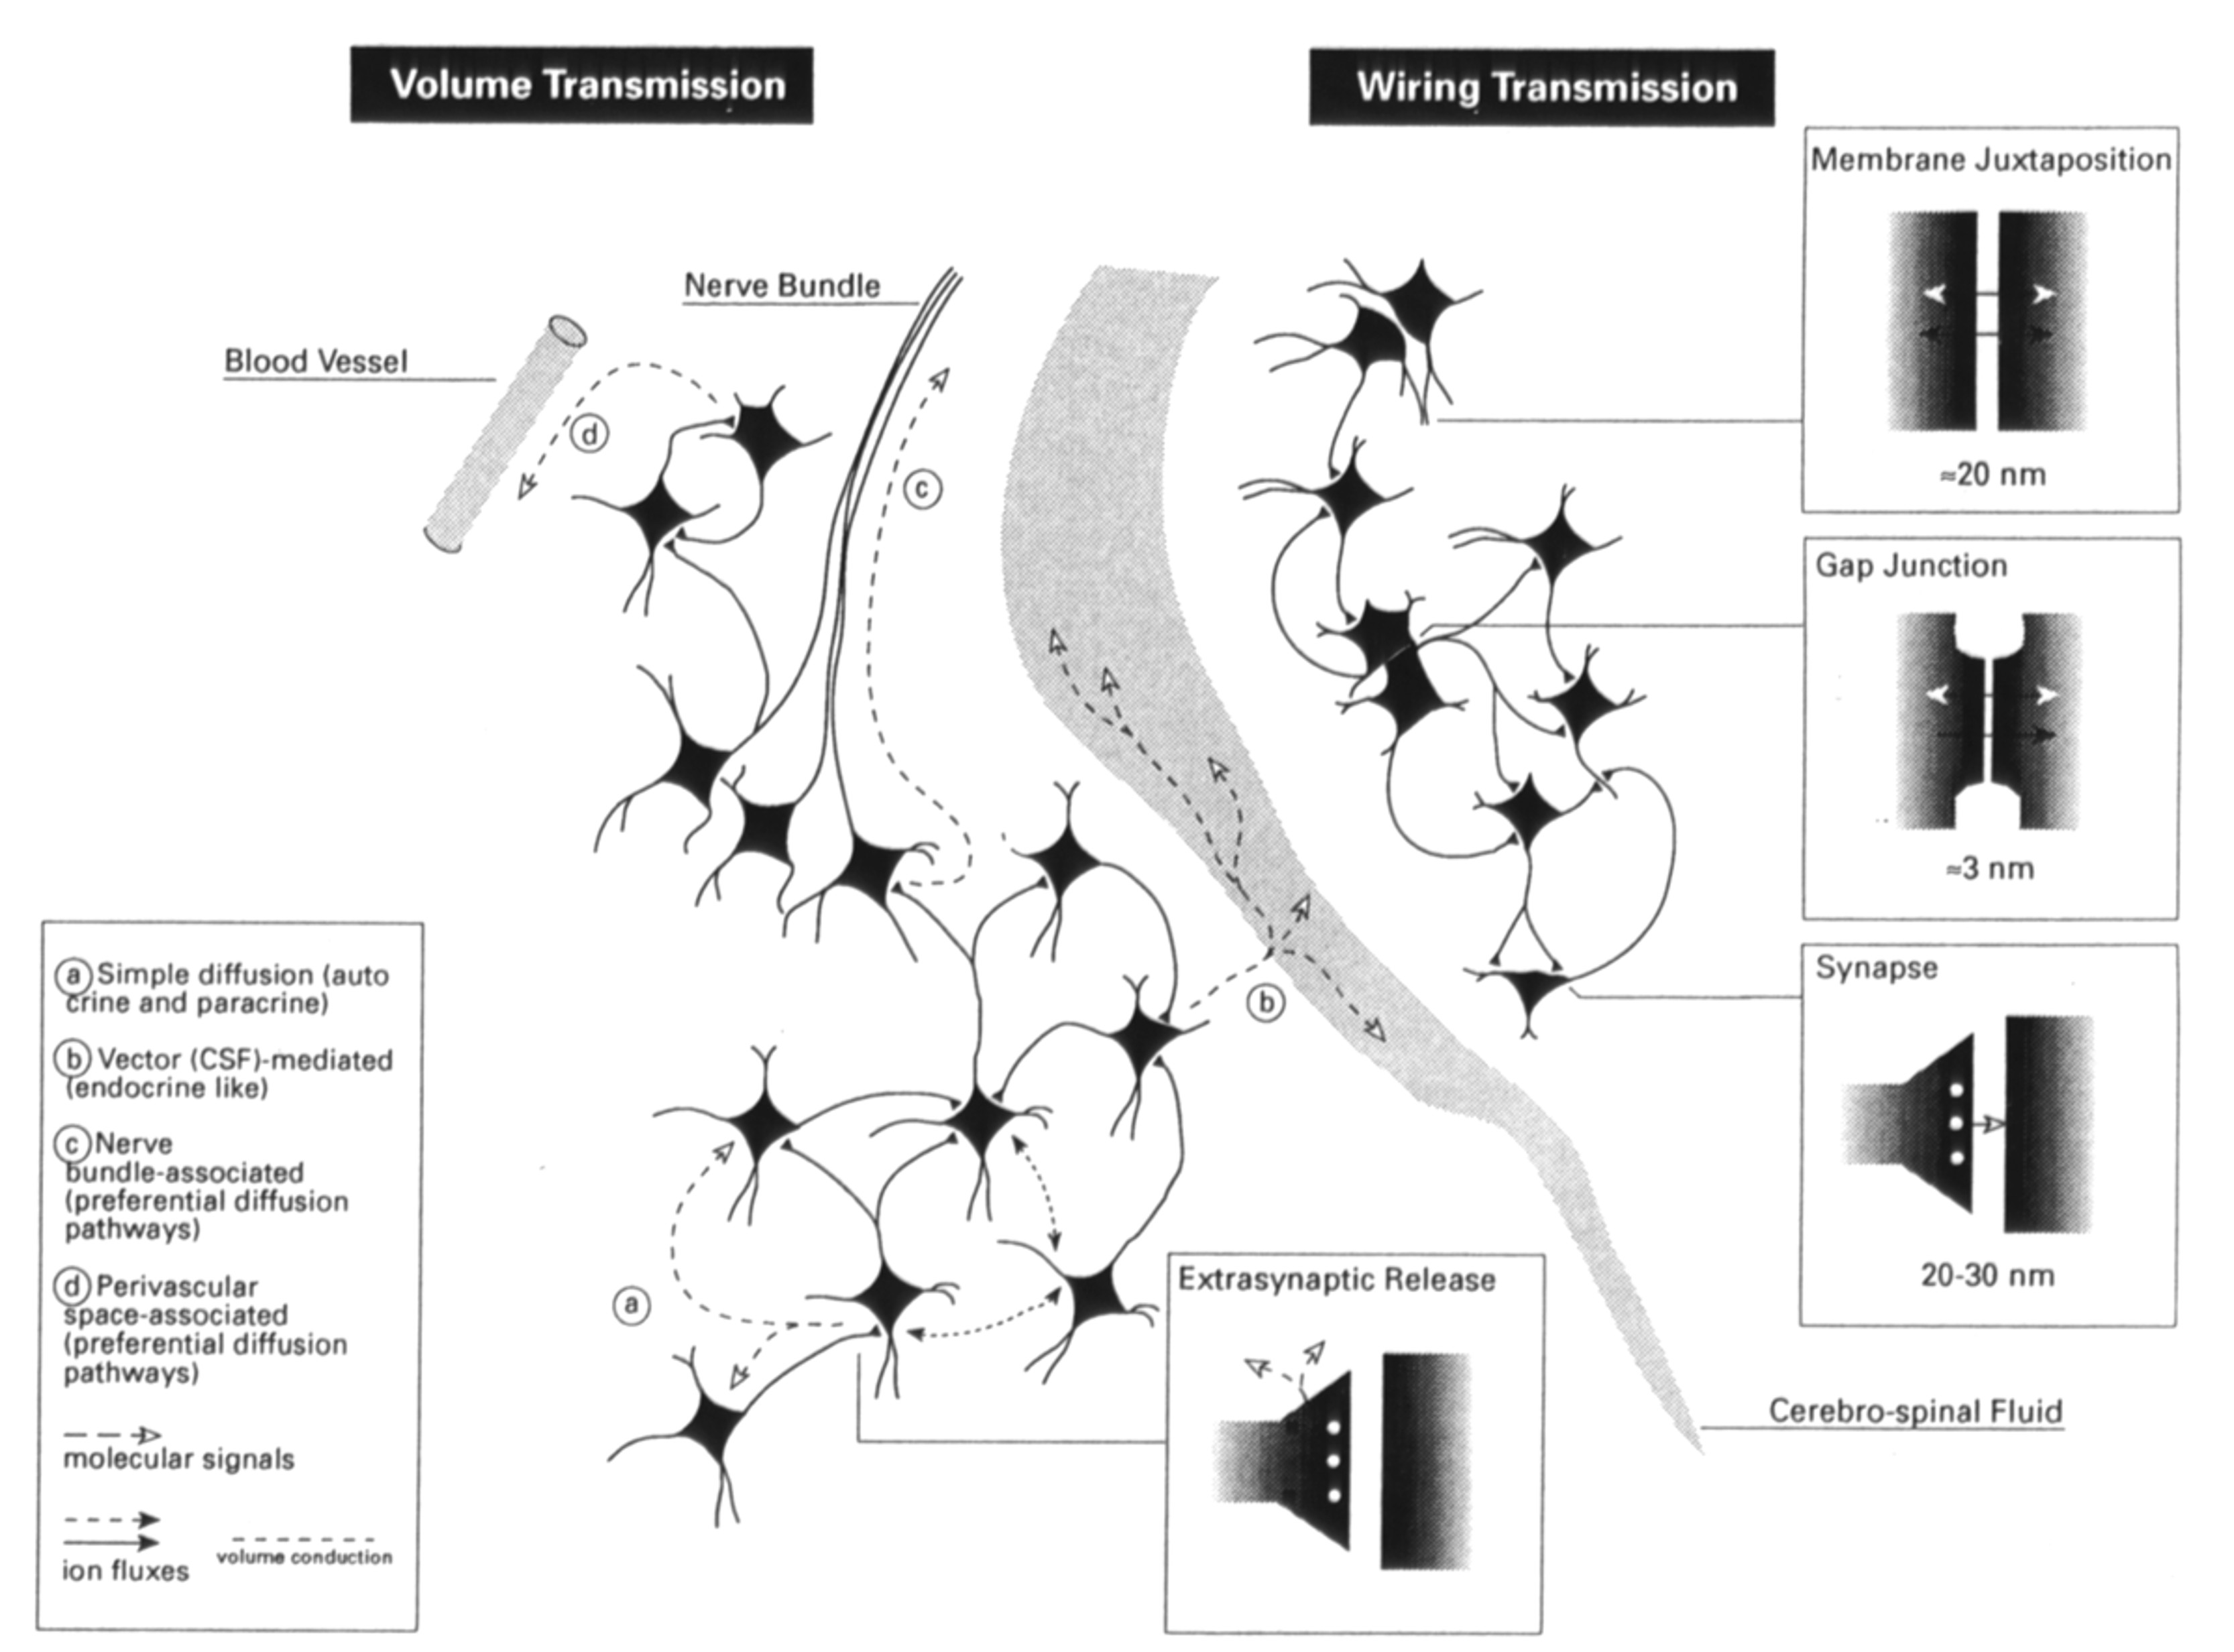
\includegraphics[width=14cm]{chapter1/figures/volTrans/volTrans.jpg}
        \caption[Illustration of the volume and wired transmission concepts]{\textbf{Illustration of the volume and wired transmission concepts.} Wired transmission operates between well defined cell pairs and mainly mediated through synapses although other structures have also been implicated (gap junctions and membrane juxtapositions). Volume transmission operates unspecifically on cell populations and is mainly mediated via diffusion in the extrasynaptic space. CSF transport and interstitial flow have also been identified as mechanisms for conveying molecular signals. Adapted with permission from \cite{agnati1995intercellular}.}
        \label{fig:introduction:volTrans}
    \end{figure}

    As stated above, VT is mainly associated with signalling molecules secreted by the source cells and sensed by the receiving ones. Nevertheless, other types of non-specific interactions have also been included in the VT family. These include interactions between ECM proteins in a `global molecular network', electrical induction between neurites (also termed ephaptic interactions) and blood pressure driven stretching of the brain tissue \cite{agnati2006volume}. Recently, it was shown that changes to the ionic composition of the extra-cellular space underlies the transition between sleep and wakefulness \cite{ding2016changes}. Such control of the the ionic concentration may also be categorized as VT.

    In the context of the system proposed in this work, we propose to categorize classical VT (i.e., VT operating via signalling molecules diffusing in the extra-synaptic) into two groups: intrinsic and extrinsic VT. Intrinsic VT refers to processes where the source cells are within the target tissue. Notable species participating in intrinsic volume transmission are GABA and glutamate. These neurotransmitters are primarily known for their role in excitatory and inhibitory WT. However, over recent decades, it has become widely recognized that many of the receptors for these transmitters, both ionotropic and metabotropic, are located at extrasynaptic locations thereby implying an ambient presence of their agonists \cite{farrant2005variations,taber2014volume}. GABA and glutamate arrive at the extrasynaptic space through a wide variety of secretion processes including synaptic spillover \cite{matsui2003ectopic,hamann2002tonic,bellamy2006interactions} and direct release through specialized transporters in neurons \cite{cavelier2005tonic}, astrocytes \cite{lee2010channel,cavelier2005DIDS} and the newly identified neurogliaform cells \cite{olah2009regulation}. All these release mechanisms dynamically operate in feedback from the activity in the network and have been implicated to be involved in information processing \cite{mann2010control,hamann2002tonic,lenk2016understanding,cavelier2005tonic}. Other well characterized species involved in intrinsic VT are adenosine \cite{wall2015localized}, ATP \cite{zhang2003atp}, endocannabinoids, neurosteroids and nitric oxide \cite{fuxe2010discovery,bellamy2000rapid} which almost all operate through specialized membrane receptors and are released from neurons and astrocytes across the nervous system. Nitric oxide is an exception as it readily crosses the cell membrane without mediation and directly operates on intracellular targets.

    Extrinsic VT refers to processes where the source cells are located outside the target tissue. Typically, these signals originate in specialized nuclei with neurons capable of producing the designated signalling molecules. These neurons innervate the target tissue and the signaling species are secreted by means of vesicle release. Since the release mechanisms employ pre-synaptic machinery it was long thought that extrinsic VT was actually WT. However, today it is well recognized that these long range nerve terminals do not form full fledged synaptic structures in the target tissue because the presynaptic machinery is typically not matched with a post synaptic receptor density \cite{taber2014volume,rice2008dopamine}. Similarly to intrinsic VT, a large proportion of membrane receptors associated with extrinsic VT signals are uniformly spread in the tissue. An extreme form of this organization is seen in the neuropeptide VT systems which include substances such as neurokinin, \textbeta-endorphin, cytokines and oxytocin \cite{fuxe2010discovery,veening2012volume}. Membrane receptors associated with these substances have been shown to exist in brain regions which are apparently not innervated by the neuropeptide producing nuclei. Indeed these substances have been shown to travel long distances in the brain, in part using the CSF, to reach the non-innervated areas and their presence in the tissue is sustained for hours following the release events. The other major family of extrinsic VT signals are the central monoamines, usually referred to as `neuromodulators' and which include dopamine (DA), acetylcholine (ACh), noradrenaline (NA), serotonin (5-HT) and histamine. The neurons producing these monoaminergic signals are located in distinct nuclei in the brain stem and basal forebrain and all show a similar organization in that they project quite densely to the entire brain \cite{gu2002neuromodulatory}. Since the rate of release and re-uptake depends on the density of pre-synaptic sites, the dense innervation pattern of these systems means that they are capable of producing rapid phasic volume signals. These systems are the topic of the next section.



    \subsection{Neuromodulator transmission and plasticity}
    The ascending neuromodulatory pathways have been drawing increasing levels of interest within the neuroscience community. Their anatomic organization is similar in that they all innervate the entire forebrain although the precise innervation pattern varies between the systems in a species specific manner \cite{gu2002neuromodulatory}. All the neuromodulators are also strongly involved in wake-sleep cycling and their levels in the forebrain decrease during sleep and increase upon awakening \cite{saper2005hypothalamic}. These systems, and particularly the dopaminergic, cholinergic and noradrenergic ones, have been shown to be important for plasticity and therefore hypothesized to be involved in cognitive processing. Their role in plasticity was first observed in classical sensory deprivation experiments where suturing one eye or denervating certain afferent somatosensory nerves would cause a reorganization in the associated cortical tissue. Damage to the neuromodulatory systems impaired these reorganizations \cite{gu2002neuromodulatory}. These three systems were also shown to affect classical \textit{in vitro} plasticity experiments where LTP or LTD are induced through controlled stimulation in paired neuronal populations. Presence of neuromodulators in the bath during such experiments have been shown to have a gating effect on the plasticity or to change the direction of the observed change \cite{zhang2009gain,yagishita2014critical,huang2012pull,otani2015dopaminergic,isaac2009hippocampal}. Correspondingly, a strong involvement of these systems was demonstrated also in behaving adults animals engaged in learning tasks. Learning is impaired by damaging these systems or gated through optogenetic control of the relevant nuclei \cite{tsai2009phasic,ogren1980evidence,hasselmo2006role}. Beyond the established role in plasticity and learning, the neuromodulators have been shown to have an acute direct effect on the activity of the network in various forebrain regions both \textit{in vitro} \cite{eytan2004dopamine,kaufman2012long,otani1998dopamine,gu2002neuromodulatory} and \textit{in vivo} \cite{tye2013dopamine,carter2010tuning,kuchibhotla2017parallel}. These changes to network dynamics have been linked to context dependent modulation of sensory processing and of behaviour. The context information provided by the modulators has been interrogated through subjecting laboratory animals to behavioral tasks while monitoring the activation patterns of the respective nuclei. Dopamine has been found to mostly convey reward and novelty information but to a certain degree also salience \cite{schultz2013updating,bromberg2010dopamine}. Acetylcholine seems to be related to conscious attention and salience \cite{pinto2013fast}. Noradrenaline has been the least studied of the three but is definitely associated with motivation and arousal \cite{carter2010tuning}. Overall, these neuromodulator systems seem to convey different but somewhat overlapping contextual information and this is used by other parts of the brain to modify behaviour accordingly and to learn the necessary associations.

    Further recent developments have provided new information as to how the neuromodulator information may be used to generate the correct associations at the circuit and synapse level. This pertains mainly to the observation that discrete rewarding events during behavioural tasks (e.g., the monkey receives a peanut) are associated with a sharp burst in the dopaminergic nucleus (VTA) and an accompanied phasic increase in the dopamine concentration in target tissue which lasts for no more than a few seconds \cite{schultz1997neural,venton2003real,arbuthnott2007space}. Given these sensor measurements and the highly extrasynaptic distribution of dopamine receptors in the tissue \cite{rice2008dopamine,taber2014volume} (also see figure \ref{fig:introduction:extVolTrans}) it seems that these are truly volume signals and therefore are not specific to a particular cell or synapse. Moreover, taking into account the significant divergence in projections from the dopamine nucleus to the rest of the forebrain, it is likely that large portions of tissue receives the same dopamine signals in synchrony. This low level of spatial but high degree of temporal specificity seem to be compatible with the notion of reinforcement learning where the reward signal does not carry in itself specific algorithmic information as to how to perform the task but the temporal presence of reward or lack thereof is implicitly used to modify the circuit appropriately. The discovery of this mode of operation for dopamine was followed by similar observations for Acetylcholine \cite{sarter2009phasic} and noradrenaline \cite{dugast2002vivo}. Thus, it is possible that all these neuromodulators support reinforcement learning based on the contextual information that they carry. These observations have spurred a vibrant debate in computational circles about how to reconcile previously described neuronal plasticity rules with the novel observations about neuromodulators. These are reviewed next.

    \begin{figure}[!htb]
        \centering
        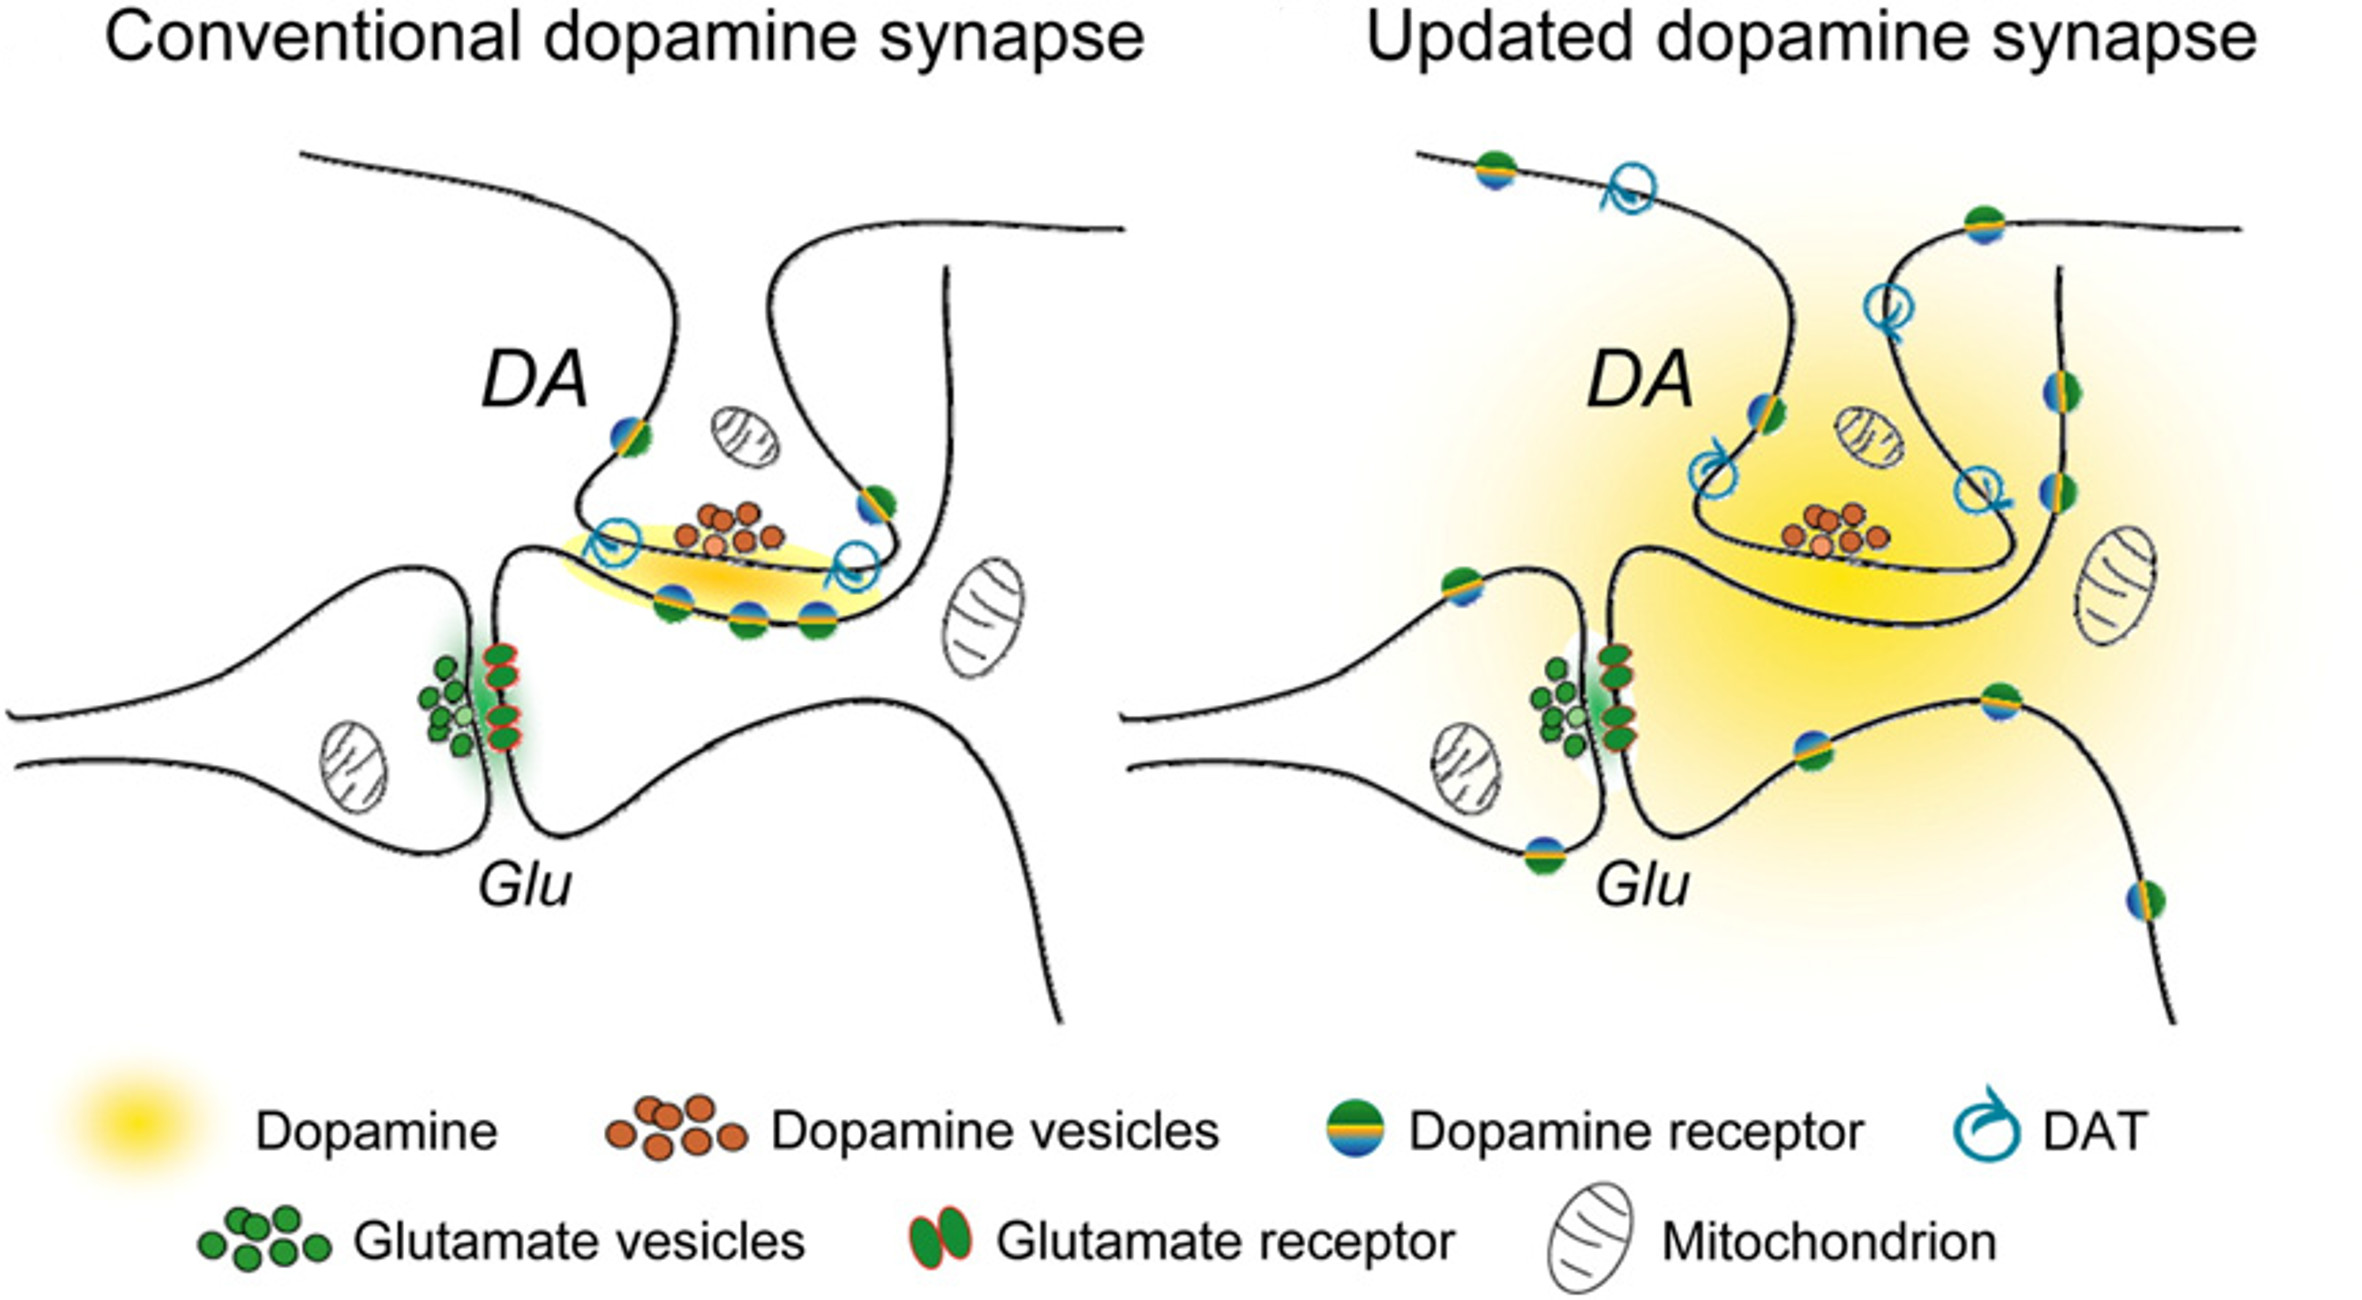
\includegraphics[width=10cm]{chapter1/figures/extrinsicVolTrans/extrinsicVolTrans.jpg}
        \caption[Volume transmission view of dopamine signalling]{\textbf{Dopamine operates as volume signal.} Dopamine and other monoamine signalling pathways have been previously considered to operate via classical synaptic transmission because they are released from nerve terminals. Recent immunocytochemistry work demonstrates that a large degree of mismatch between the locations of monoamine release sites and their respective receptors. This mismatch is taken a evidence that these systems operate in volume transmission mode. Adapted with permission from \cite{rice2008dopamine}.}
        \label{fig:introduction:extVolTrans}
    \end{figure}

    \label{sec:introduction:neuromodulators}
    \subsection{The Izhikevic thought experiment}
    For many years, since the influential work of Donald Hebb \cite{hebb1961organization}, neuroscience had essentially just a single learning rule at its disposal. That was the Hebbian plasticity rule which states that ``neurons that fire together, wire together''. This originally hypothetical concept was later proven experimentally \cite{bliss1973long}. This rule was later adjusted to account for the need to also reduce the strength of connection and to align with various experimental observations \cite{caporale2008spike,bi1998synaptic}. One of the generally accepted forms of this rule is the spike timing dependent plasticity (STDP) which asserts that a synapse would be strengthened when the presynaptic neuron had fired shortly before the post synaptic one. Alternatively it would get weakened if the temporal coupling had been reversed. The correlations required for this form of plasticity are variable but are generally in the order of tens of milliseconds. This form of plasticity is well established experimentally \textit{in vitro} and has been able to account for some connectivity features observed in the nervous system. However, making computational models of higher level learning and memory is difficult when using it on its own \cite{brea2016does}. Incorporation of reinforcement learning principles in computational theories has allowed generation of models of episodic and associative memory \cite{brea2016does} and even of goal directed behaviour that requires learning \cite{brea2016does,fremaux2013reinforcement}. Thus the notion of a neuromodulator carried reinforcement signal is a major step forward in the theoretical understanding of cognitive processing. The computational work in this context usually assumes the presence of a low level mechanism whereby the classical STDP rule is modulated by the concentration of dopamine so as to allow plasticity to occur at the appropriate part of the circuit. Several forms of this mechanism have been suggested (reviewed in \cite{fremaux2015neuromodulated}) and we will next present one prominent example for such a formulation, suggested by Izhikevich \cite{izhikevich2007solving}.

    Izhikevich was concerned with the fact that rewarding events in the real world are a product of behaviour (e.g., a toddler trying to open a box of candy) and  therefore operate at very different time scales and usually arrive in delay as compared to the neuronal activation pattern that generated them. The question of how to link variable rewarding events to preceding neuronal activation is sometimes termed the `distal reward problem'. Izhikevich suggested thats STDP events, i.e., spikes occurring in both the pre- and post- sides of a synaptic pair at close temporal proximity, do not immediately elicit plasticity as originally formulated in the STDP principle, but actually initiate an `eligibility trace' which decays at a time constant of several seconds. The activated synapse would then only be reinforced if a dopamine flux arrives before its eligibility trace has decayed completely (figure \ref{fig:introduction:izhi} A-C). Based on this principle, a rewarding event would reinforce all the synapses that participated in preceding spiking activity within the eligibility trace time scales. This may mean that synapses that have been active by chance due to unrelated network activity would also be indiscriminately reinforced. However, over several repeats of the task (and consecutive rewarding events) only the synapses that are instrumental in obtaining of the reward would have been consistently activated just before it. These synapses would be significantly reinforced as compared to the other, opportunistically activated, ones. This notion is presented in figure \ref{fig:introduction:izhi} D-E which shows raster plots of activity in a simulated network of 1000 neurons. The network is subject to 100 different random stimulation patterns where a single action potential is simultaneously induced in a specified set of 100 neurons. These stimulation patterns are applied in random order but only S\textsc{1} is consistently followed by a dopamine reward pulse which occurs 1-3 seconds later. The plots show that, even though many of the stimulation patterns have been applied between S\textsc{1} and the reward, the network response following an S\textsc{1} stimulation was significantly potentiated compared to all other patterns.

    \begin{figure}[!htb]
        \centering
        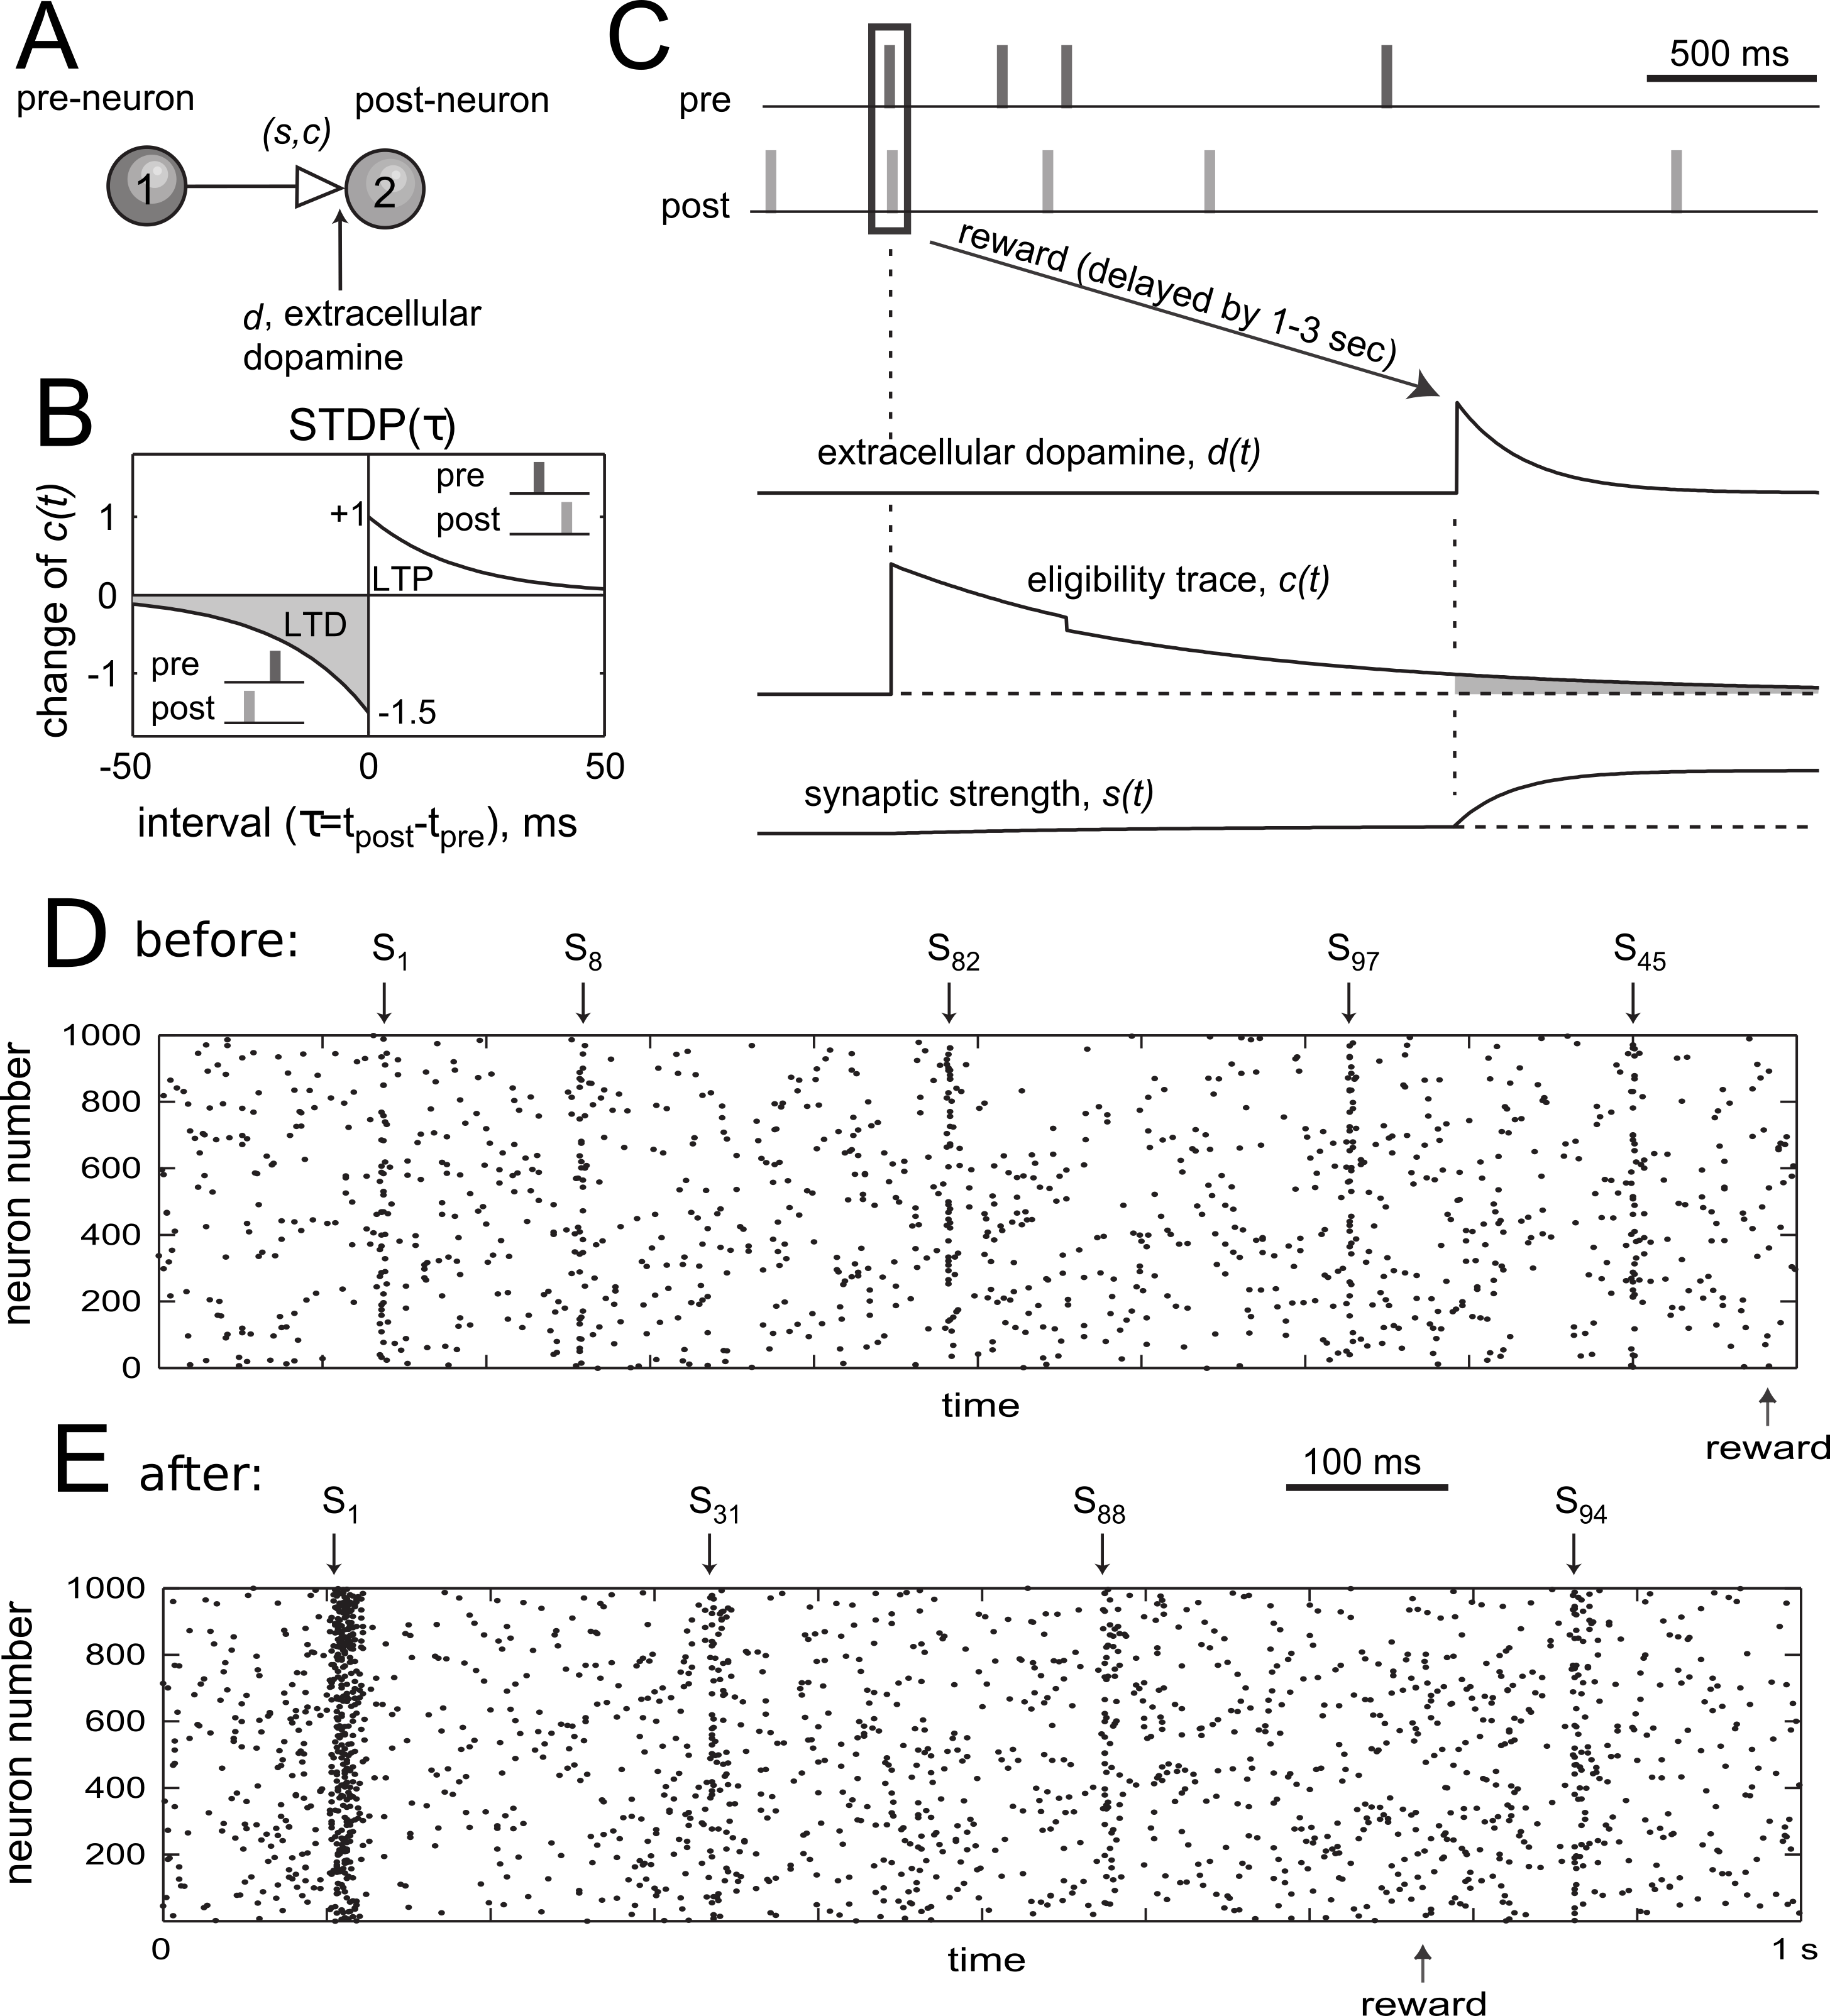
\includegraphics[width=12cm]{chapter1/figures/izhiIllustration/izhiIllustration.png}
        \caption[The Izhikevich proposal for a plasticity rule involving dopamine]{\textbf{According to Izhikevich's proposal, dopamine interacts with the classical STDP rule via eligibility traces.} (A) Illustration of the basic computational unit: a pre-post neuron pair with parameters holding the strength of the synapse between them (s) and the state of the eligibility trace (c). A third parameter (d) holds the level of extracellular dopamine. (B) A classical STDP rule is applied with regards to the timing of firing in the pre and post neurons to inform the eligibility trace rather than the synaptic strength. (C) Demonstration of the plasticity rule operating over a stretch of network activity. A pre-then-post firing event at a high temporal proximity causes an increase in the eligibility trace. Arrival of dopamine before the trace has completely decayed results in potentiation (increase in the parameter s). (D-E) Demonstration of how dopamine signalling can induce pathway specific plasticity despite operating as a volume signal. 100 different stimulation patterns are defined and applied continuously to the network. Only pattern S1 is consistently followed by a dopamine reward and is the only one to be potentiated. Adapted with permission from \cite{izhikevich2007solving}.}
        \label{fig:introduction:izhi}
    \end{figure}

    This Izhikevic thought experiment illustrates how a non-specific reward signal may interact with the activity and with established plasticity rules to reinforce just the parts of the circuit that are relevant for the task. It also highlights the importance of having a temporally narrow phasic signal to facilitate the selection of the correct synapses. Nevertheless, the mechanism suggested by Izhikevic as well as other proposals by computational neuroscientists \cite{fremaux2015neuromodulated} are all purely hypothetical and have not been established experimentally. This is mainly due to the absence of \textit{in vitro} systems that are able to control and monitor both the spiking activity in a neuronal circuit and the phasic neuromodulator signals applied to it. One such system has been recently proposed by Yagishita et. al. \cite{yagishita2014critical}. That system was based on a brain slice which includes both the main dopamine nucleus (VTA) and the striatum. The activity in the VTA was controlled via optogenetic activation, the spiking activity of specified striatal spiny neurons was controlled by directly patching them and specific synaptic spines were artificially activated by means of glutamate uncaging. This system was used to prove the hallmarks of the Izhikevic model, namely, that a synaptic activation coupled to an action potential in the post synaptic cell results in a potentiation only when followed by activation of the VTA within a stringent time window of about 1 second. Such slice based systems are indeed an attractive way to study the low level mechanisms by which neuromodulators interact with the activity and plasticity but they also suffer from a few drawbacks. Firstly, since they are based on a single tissue section they cannot incorporate more than a single neuromodulator nucleus into the same experiment and hence will not be able to investigate how different modulatory species, which are all important for plasticity and for the activity patterns in awake animals, interact with each other. Secondly, the slice system generates neuromodulatory pulses indirectly through stimulation of the relevant nucleus so they do not control the precise concentration of neuromodulator in the tissue, which has been shown to gate the plasticity in a non-trivial fashion \cite{otani2015dopaminergic}. In the next section we propose a culture based system that will address the experimental gaps.

    \label{sec:introduction:izi}

    \section{Proposed system and how it addresses present experimental gaps}
    To address the experimental shortcomings described above we propose to extend the established functionality of neuronal culture grown on MEAs with a rapid solution exchange functionality allowing application of neuromodulatory pulses onto an entire neuronal circuit at time scale of phasic volume transmission. As explained in the previous sections, both the latency in the pulse arrival and the its width are thought to be important parameters in the functioning of the neuromodulator system and for using it to achieve reinforcement learning. Thus it is crucial that the system allows for the agonist to arrive at the cells and be removed within no more than a few seconds. Such a functionality can only be supported by a neuronal culture and not by slices. The reason for this is that brain slices are normally \(150-300 \mu m\) thick so even if the solution around them were to be replaced very fast, additional diffusion into the tissue would be required which, given its thickness, would take more than a few seconds. In the case of neuronal culture, which forms a thin monolayer of no more than a few microns, such a diffusion bottleneck would not arise. An important part of the requirement is that the agonist pulse would span the entire culture as this spatial non-specificity is a conspicuous feature of the volume transmission process. Luckily, neuronal culture technology makes it far easier to restrict the tissue size in par with the requirements.

    The proposed system, if realized, would be able to readily employ any type of agonist or even combinations to test for interactions. Additionally, these experiments would be concentration-resolved because the extracellular solution would be directly manipulated. This aspect of the system would be useful if the precise agonist concentration values were to be of concern. A striking characteristic of the neuromodulator signalling is that, beyond the plasticity, it also elicits a direct effect on the activity in the target circuit. It is yet unknown how these seemingly distinct processes are coded for by the same neuromodulator species but it is plausible that the code has to do with tonic and phasic aspects of the signal which produce different agonist concentrations in the tissue. It is worthwhile to note that achieving rapid control over the extracellular chemistry could also be useful for studying intrinsic volume transmission processes. However, these processes are produced by localized secretion events within the tissue and therefore result in more spatially complex signals as compared to the extrinsic ones. Consequently, modelling intrinsic volume transmission might require a system that goes beyond simple solution exchange and allows generation also of spatially complex agonist patterns. Nevertheless, the system of concern here will hopefully serve as a proof-of-principle and hopefully pave the way for future more complex designs.

    Basing the system around neuronal culture would also provide access to the other advantages of the culture system which include, as described in section \ref{sec:introduction:achievements}, a growing ability to control the network architecture and to perform experiments over long stretches of time and thus allowing more complex learning paradigms to be explored. Finally, much of the theoretical computational studies, and especially those concerned with generic properties of neural circuits, employs simulated networks that are initially randomly connected (e.g., the above-mentioned Izhikevic model). Randomly organized neuronal cultures therefore comprise a natural experimental partner to these kinds of simulation data. In the next section we will review the technology that will be used to implement the rapid solution exchange.

    \section{Rapid solution exchange with microfluidics}
    Rapid solution exchange in neuroscience has been widely implemented via iontophoresis (e.g., \cite {jonas1993quantal,hestrin1992activation}). This application method ejects charged agonists from a tip of a micropipette by applying an electric potential to the fill solution. Although this technique is able to generate agonist transients at extremely fast time scales (sub millisecond), it is limited in its spatial scale and can only generate significant concentration increases around a single synapse or at most a single cell soma.

    The recent advent of microfluidic technology offers an exciting way for precision control over movement of liquid in an on-chip fluidic network. Microfluidic devices are typically fabricated with soft-lithography techniques (see section \ref{sec:methods:fabrication}) and consist of a network of flow channels each at the scale of several to hundreds of microns at most. The basis for the success of microfluidics is that the flow operates purely at the laminar flow regime. In macro-scale flow systems, due the larger dimensions and increased flow velocities, the internal inertial forces in the liquid greatly dominate the viscous ones and this results in a turbulent flow regime \cite{fluidBook}. This regime is characterized by localized turbulences, unexpected fluctuations and significant mixing between different parts of the liquid. The ratio between inertial and viscous influences is known as the Reynold's number (\(R_{e}\)) and turbulent flow occurs for \(R_{e}>10^{3}\). For lower \(R_{e}\), which is the case for microfluidic chips, the viscous influences dominate and the flow becomes smooth and predictable. In this regime, the flow forms separate liquid layers (lamina) which do not mix, hence the name laminar flow. Regardless of the input configuration, laminar flow always organizes in a simple axial configuration and is completely deterministic which allows the design of chips with programmatic routing and mixing of solute molecules and with accurate control of their spatiotemporal concentration profile. Most microfluidic systems are characterized by a particularly low Reynold's number, \(R_{e}<1\), which corresponds to the creeping flow regime. In this regime, the flow is well modeled by a version of the Navier-Stokes equations where the inertial term is completely neglected allowing simple analytical solutions. One important consequence of this is that the flow velocities in creeping flow always follow a parabolic profile which makes it easy to estimate shear stresses along the vertical axis.

    A renowned application of microfluidic technology is the flow focusing device \cite{takayama2001laminar}. This device comprises a main channel with three input ports in a fork-like design (i.e., they all share the same split point at the top of the main channel). The central input port carries an agonist molecule where as the side ports carry blank media. Because of the laminar flow, the streams originating from the different ports do not mix and the extent of diffusion that occurs between them as they proceed down the channel can by controlled via the flow velocity. By accurately adjusting the relative flow rates of the three streams the width of the central (agonist) one and its position across the channel may be accurately controlled. In this way, the agonist can be applied to very specific locations with subcellular resolution. Such subcellular localization is similar in performance to iontophoretic application. However, in contrast to iontophoresis, this approach may be readily adapted to larger tissues as the scales merely depend on the device geometry and on the flow rates and how they are controlled. This is the basis for our agonist pulsing device, described next.

    This Ph.D work will utilize a y-shaped (2 input ports) microfluidic device with one port carrying the agonist and one carrying blank media. At baseline, the flow rate of the blank stream will be significantly higher than that of the agonist stream so the latter will be restricted to a small side section. When a pulse command is issued, the flow rates will be temporarily flipped so that the agonist stream will be pushed across the channel in place of the diminished blank stream. When the flow rates switch back, the streams will revert back to the baseline arrangement but this will result in an agonist pulse traveling along the channel and in a temporary exposure of the cells to it (figure \ref{fig:introduction:intShift}). Such sweeping back and forth of a flow stream is termed interface shifting \cite{bae2009rapid}. In this way agonist pulses can be generated that encompass practically the entire channel cross section. In chapter \ref{chap:microculturePulses} we will show that this approach may be used to successfully mimic the temporal exposure profiles of phasic neuromodulator signalling. This application of microfluidics to neuronal studies highlights the great potential that this technology holds for neuroscience questions that involve extracellular species. Nevertheless, microfluidic applications to neuroscience, and in particular those involving flow, are still at their infancy, as reviewed in the next section.

        \begin{figure}[!htb]
        \centering
        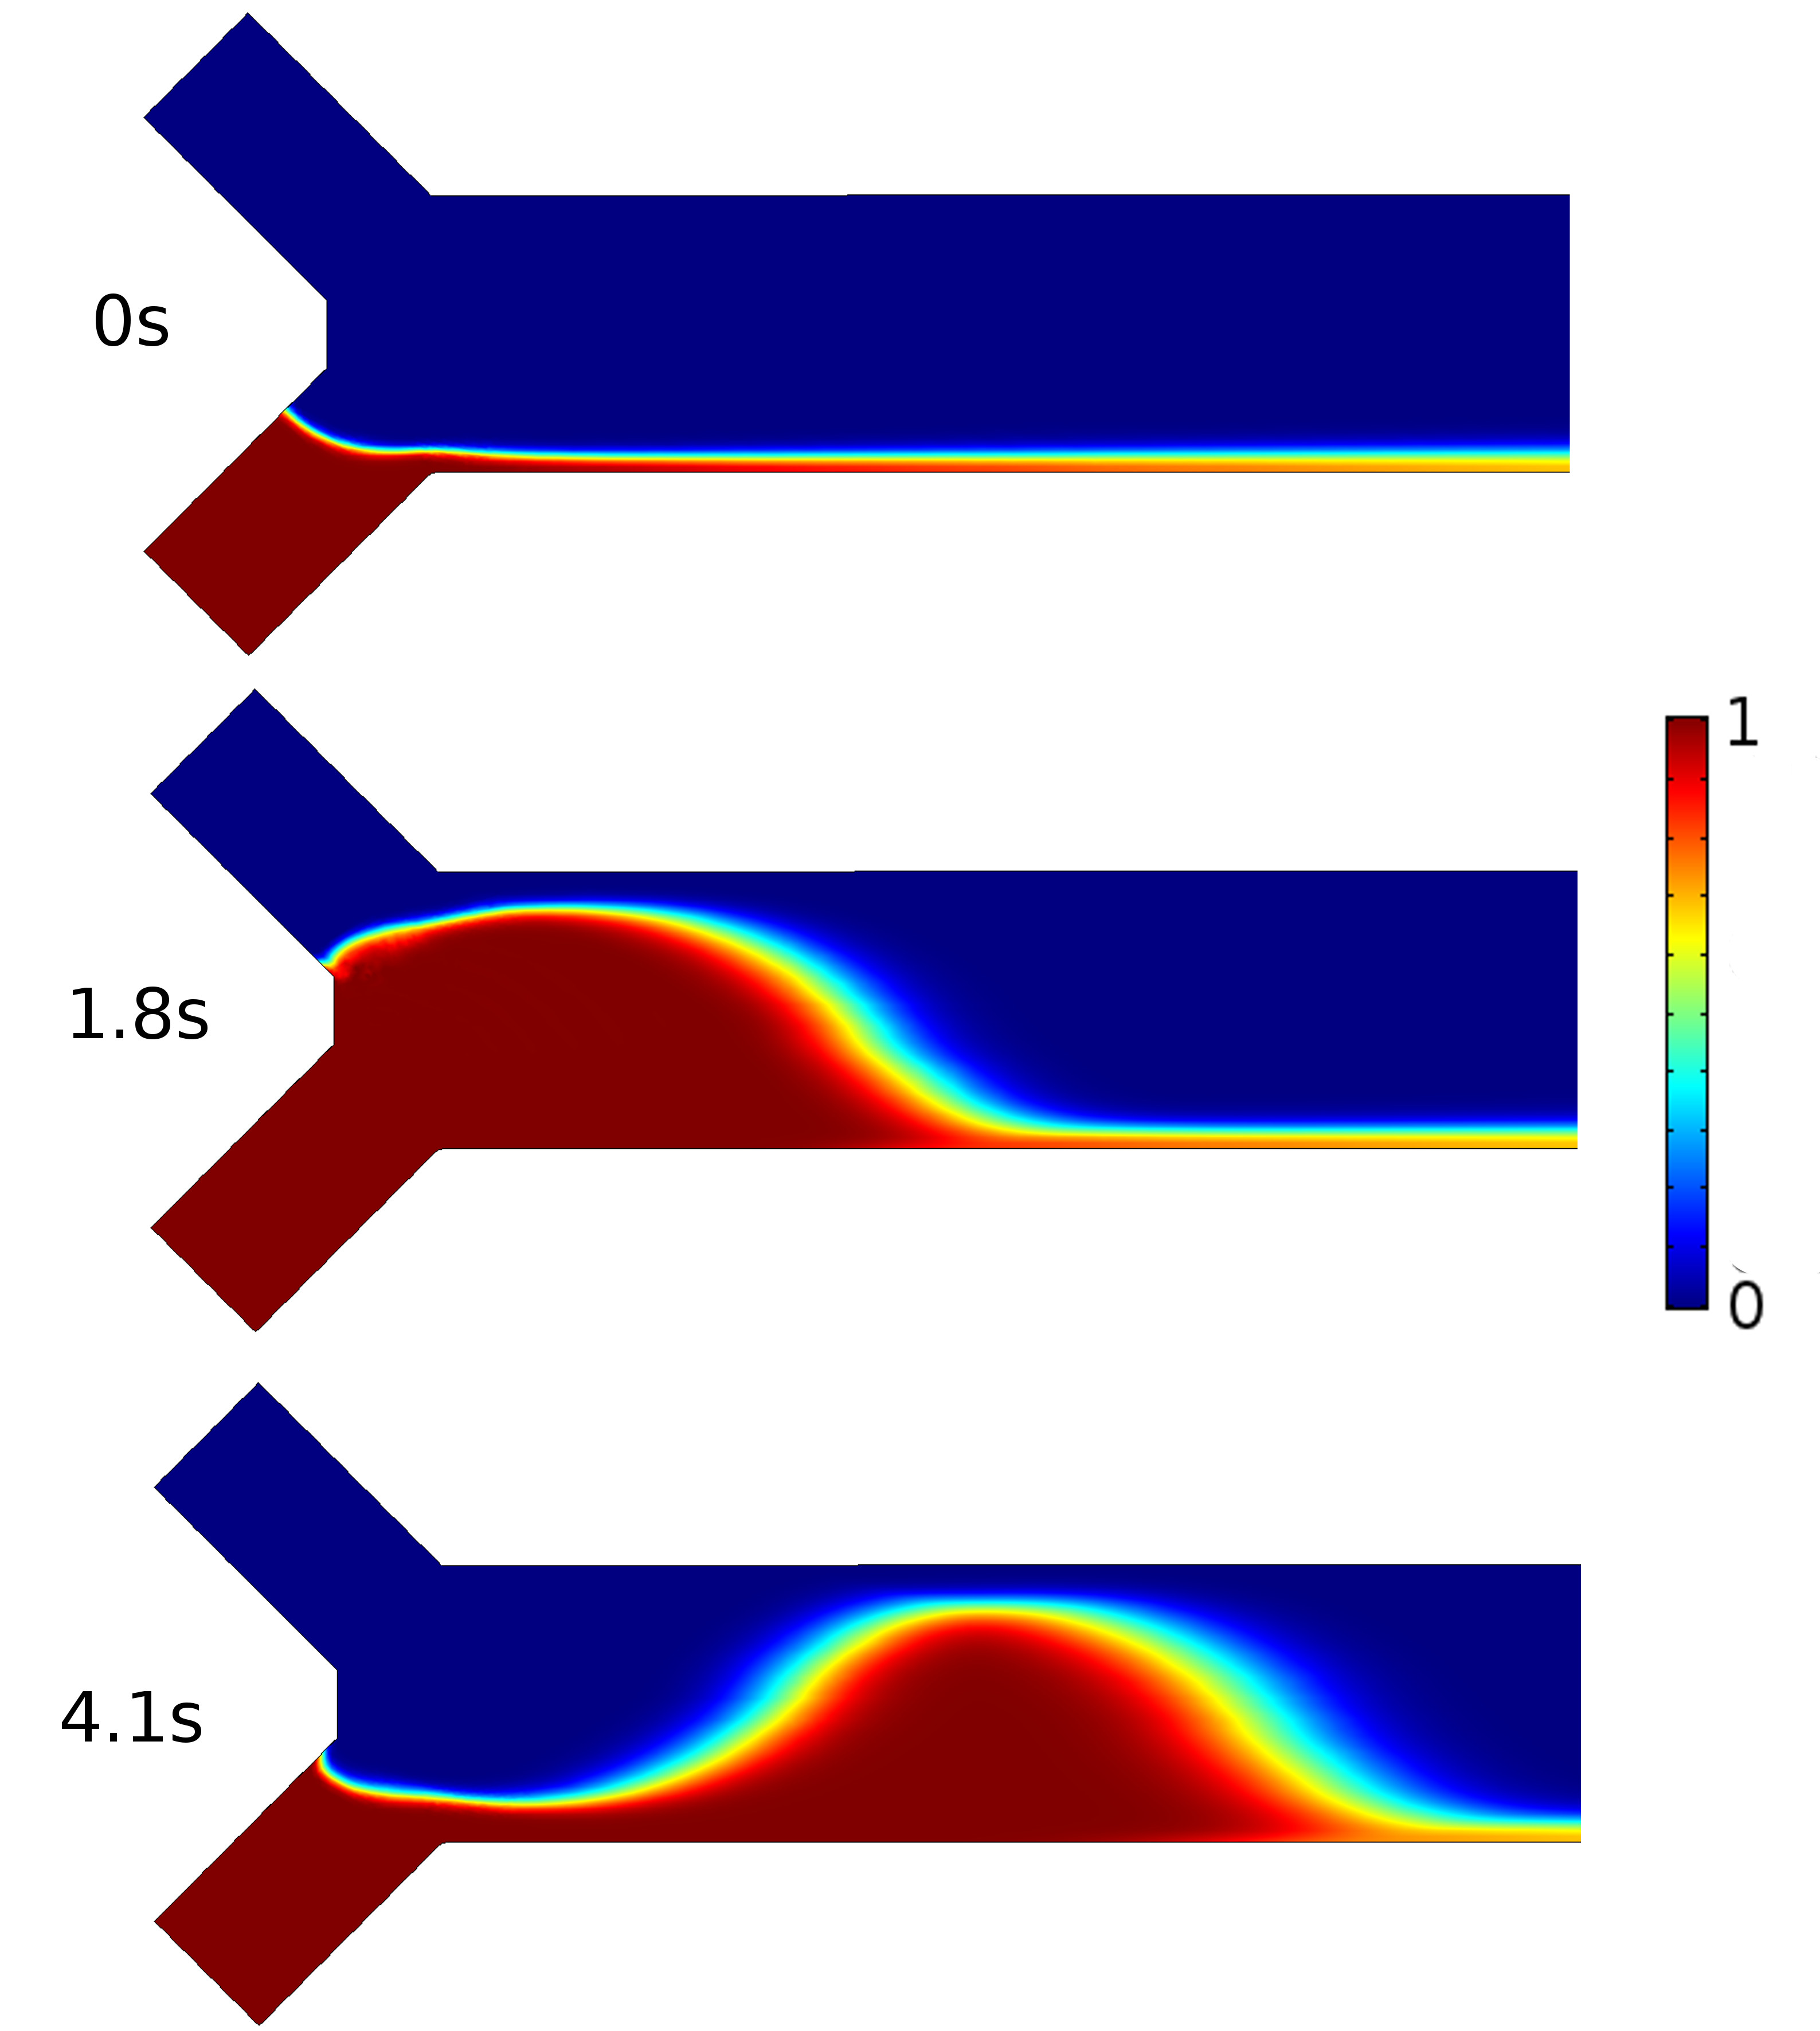
\includegraphics[width=12cm]{chapter1/figures/intShift/intShift.jpg}
        \caption[Generating a pulse with the interface shifting method]{\textbf{Flipping between the flow rates in the input ports generates an agonist pulse.} Red color depicts the agonist stream whereas the blue depicts the blank stream. Flow rates are initially unbalanced in favour of the blank stream but flipped momentarily upon a pulse command. This results in sweeping of the interface back and forth and generating of an agonist pulse travelling down the channel. These images were produced by a finite element simulation used to characterize the pulsing performance in chapter \ref{chap:microculturePulses}. Color scale shows normalized concentration (1 in agonist stream and 0 in the blank stream).}
        \label{fig:introduction:intShift}
    \end{figure}
    \label{sec:introduction:mufdDrugDelivery}

    \subsection{Microfluidics in neuroscience}
    Microfluidics technology has sprung into the neuroscience psyche with the introduction of the innovative compartmentalized culture system by Taylor et. al. \cite{taylor2005microfluidic}. Taylor's device, a.k.a. `Taylor's ladder', comprises two large scale compartments that are connected by small rectangular tunnels which are only \(1 \mu m\) high and wide. A neuronal culture seeded into one of the compartments are constrained to that side because the tunnels are too small for cell somata to go through. Axons, however, are able to traverse the tunnels by virtue of their smaller dimensions and so, after a few days, the unseeded compartment become inhabited with axons only. This arrangement allows pharmacological and molecular biology assays to be conducted only on the axons. This unique compartmentalization of neurons has enabled breakthrough research into the localization of biological markers within the neuron with important consequences to cell signalling and developmental neurobiology. This work demonstrates the major usefulness of microfluidic technology in achieving topological control and was extended by many others. These further work include compartmentalization of synapses \cite{taylor2010microfluidic}, of co-cultures \cite{robertson2014chemically,renault2015combining} and even of multiple cell populations with directional connectivity between them \cite{peyrin2011axon,honegger2016microfluidic,dauth2016neurons}. Evidently, the compatibility of microfluidic devices with neuronal culturing has been well established but also found to be more challenging than in standard conditions due to the involved materials and the imposed chamber geometries \cite{millet2007microfluidic}.


    \label{sec:introduction:mufdNeuroscience}
    \subsection{Neurons and flow}
    The above-mentioned neuroscience applications mainly utilized the fact that microfluidic technology involves rapid prototyping of micro-structures with bespoke designs. However, the main aspect of the technology, rapid and precise fluid and solute handling, has hardly been tapped as far as neuroscience applications are concerned. This despite the potential of such applications to study aspects of the neuronal volume transmission. A likely cause for this disregard is probably that neurons are considered to be extremely sensitive to mechanical perturbations and to shear stress, so such experiments might be expected to be difficult. Indeed some of the studies that did employ microfluidic flow incorporated shear protection measures to try and circumvent this issue \cite{wang2008microfluidics,morel2012amplification}. These studies were indeed able to perform elegant experiments involving generation of growth factor gradients around developing neurons to attract or repel their growth cones. However, they did not show data to demonstrate that the shear protection was required and seemed to take its necessity for granted. Another recent work seemed to contradict the shear sensitivity notion as it reported that primary rat neurons may be subjected to very high shear for over 24 hours without adverse effects \cite{liu2013galanin}. Overall, the effect of shear stress on the function and viability of neuronal culture has not been systematically studied and is poorly understood. Nevertheless, understanding the shear limitations is critical if the full potential of flow microfluidics is to be realised for neuroscience studies. In this context, it is important to mention some reports of neurons developing for long term in culture under very slow gravity fed microfluidic flow, where the magnitude of convection is comparable to diffusion so shear is not a factor \cite{choi2013neurotoxic,millet2007microfluidic,kumamoto2015effects}. This Ph.D work is concerned with much faster flow rates and will provide novel data regarding the viability of neuronal culture in such conditions. Additionally, all the above-reported work did not included any kind of electrophysiology under flow so it is altogether unknown how it affects the network activity. Possible influences could involve activation of stretch receptors or interaction with intrinsic volume transmission processes in the tissue. Thus, the inclusion of micro electrode arrays in the system proposed here will also serve to provide novel data regarding the spiking network activity under flow.
    \label{sec:introduction:neuroFlow}

    \section{Ph.D objectives}
    In the preceding sections, we identified gaps in current \textit{in vitro} neuroscience experimental platforms given recent developments in neuromodulator signalling. To address these gaps we proposed a system combining the technologies of neuronal culture, microelectrode arrays microfluidics. We further described the state of the art of these technologies and the technical hurdles that still need to be overcome. Thus, we are now in position to define the goals of this Ph.D work. The main goal is the development of a system for rapid solution exchange to an entire neuronal culture at time scales matching phasic neuromodulator signalling with a concurrent measurement and control of network spiking activity. To achieve this goal we will traverse 4 subgoals accounting for the main technical steps that need to be ascended. These subgoals match the experimental chapters of this thesis:

    \begin{enumerate}
    \item Establish gold standard neuronal culture recording and stimulation using MEAs. In this chapter we will also attempt to induce plasticity in the network in conjunction with slow bath application of dopamine. This will serve as motivation for the further integration with microfluidics.

    \item Establish a long term neuronal culture in microfluidic devices at the desirable geometry and assess its viability under the required flow rates.

    \item Characterize the stability of the spontaneous and evoked network activity under flow at the required flow rates.

    \item Combine all the lessons learned in the previous steps to build a working prototype of rapid solution exchange to an entire neuronal culture at the time scales of phasic neuromodulator signalling. Demonstrate the functionality of model by pulsing dopamine in conjunction with applying stimulations to the network.
    \end{enumerate}


    \label{sec:introduction:objs}


%\chapter{Methods}
\label{chap:methods}



	\section{Basic fabrication elements}
    This section provides protocols for the basic fabrication building blocks put together in the construction of the different devices used in throughout this Ph.D work. Specific protocols for the assembly of such particular devices are further provided in the relevant chapters.

    \label{sec:methods:fabrication}
        \subsection{PDMS preparation}
        PDMS pre-polymers (Sylgard 184, Dow Corning) were mixed in the ratio 10:1 w/w base monomer to cross-linking catalyst, and de-gassed in a desiccator unit attached to a vacuum pump. The resulting viscous liquid was poured onto a mould or a substrate depending the application and de-gassed again if required. The PDMS was cured at 60-80\degree C for 2 hours or overnight.
        \label{sec:methods:PDMSMix}


        \subsection{SU-8 Embossing}
        To create microchannel moulds a thick film photoresist was required. SU-8 is known to allow features of high aspect ratio and vertical sidewall, both essential for microchannel fabrication. SU-8 film thickness is primarily determined by spin-coater speed and time, and by the ratio of solvent to epoxy in the photoresist. The higher the epoxy content, the more viscous it will be and more resist will remain after the spin-coating and heating steps described below.

        A 3 inch (\(76.2mm\)) silicon wafer was sonicated for 5 minutes in ethyl lactate and then rinsed in more of the same solvent. This process was repeated for acetone, methanol, and IPA. The wafer was dried under a nitrogen stream and dehydrated at 150\degree C for at least 30 minutes. SU-8 2050 was deposited onto the centre of the wafer and spun at 500rpm for 10 seconds to coat uniformly, followed by 30 seconds at 2000rpm to thin the photoresist to \(\approx 75\mu m\). The wafer was baked on a 65\degree C hotplate for 5 minutes followed by 95\degree C for 10 minutes, to remove all solvent from the photoresist.

        Photomasks of chrome on soda glass were designed using a CAD software (Autodesk Inventor Professional) and fabricated by JD Photo-tools Inc. Such designs of 2-port and 3-port channels are provided in figure \ref{fig:devices:basicDimensions}. After aligning the mask, the baked wafer was exposed to UV light at \(365nm\) and \(9\frac{mW}{cm^{2}}\) for 30 seconds. The exposed wafer was heated again for 5 minutes at 65\degree C and 10 minutes at 95\degree C, to cross-link the exposed regions of the SU-8. The wafer was immersed in ethyl lactate with mild agitation for 15 minutes, to strip off the unexposed SU-8 from the wafer. After rinsing with more ethyl lactate, the wafer and SU-8 features were heated to 150\degree C for 30 minutes and allowed to cool, in order to render the photoresist mechanically robust (hard bake). Measurement of the SU-8 features with a contact profilometer confirmed the height to be between \(60-100\mu m\).

        After the hard bake, the wafer was thermally glued (Epo-Tek) to a machined disk of aluminium \(76.2mm\) in diameter and \(2mm\) thick. This provided rigidity to the wafer, greatly reducing the possibility of it shattering if exposed to a flexing force during subsequent PDMS degassing and excising steps.
        The gluing process took 20 minutes on a 115\degree C hotplate. This temperature was chosen to ensure the SU-8 features were not reheated close to their glass transition point.
        \label{sec:methods:SU8}

        \subsection{Soft lithography}
        PDMS pre-polymers were mixed and degassed (section \ref{sec:methods:PDMSMix}). The pre-ploymer mix was then poured into a polystyrene petri dish containing a silicon wafer patterned with SU-8 (section \ref{sec:methods:SU8}).
        The PDMS was cured at 60\degree C for at least 2 hours or overnight at room temperature. After this time the PDMS was peeled off the mould and individual dies were separated with a scalpel. Fluid access ports were created with a \(0.5mm\) biopsy punch (ProSciTech), flushed with deionised water to remove debris, and nitrogen dried. The moulded face of the PDMS was cleaned \(3\times\) with scotch tape to remove remaining debris and dust. The process is illustrated in figure \ref{fig:methods:softLithography}.

        \begin{figure}[h]
            \centering
            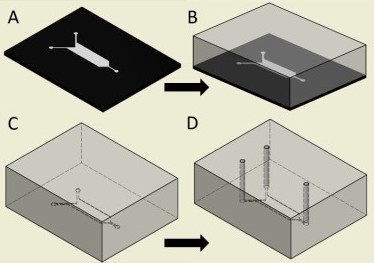
\includegraphics[scale=0.7]{chapter2/figures/softLithography/softLithographyProcess.jpg}
            \caption[Illustration of the soft lithography process]{\textbf{Illustration of the soft lithography process.} The SU-8 master mould (A) is covered with liquid PDMS (B). After curing at 60-80\degree C for 2 hours, the PDMS is excised with a scalpel and peeled from the mould (C). Access ports are cut with a biopsy punch (D). Figure was adapted from \cite{johnstoneThesis} with permission.}
            \label{fig:methods:softLithography}
        \end{figure}
        \label{sec:methods:softLitho}
        \subsection{Thin film spinning}
        To generate thin films of PMDS, the mixed pre-polymers were poured onto the central third of either a 3 inch (\(76.2mm\)) silicon wafer or a \(80\times 80 mm^{2}\) glass slide and processed on a spin-coater (SPS Europe Spin 150), with film thickness determined by spin RPM and time. The substrate with the pre-polymer film was then transferred to a hotplate at 100\degree C and baked for 5 minutes, to harden the PDMS film and heat the substrate. Next, we applied a grid of thick PDMS strips to the top of the thin film. Due to the high temperature of the substrate the PDMS strips did not spread and hardened immediately thus forming think tabs around rectangular PDMS sheets which were cut out and used as the microwell layer in specific device designs. The thick tabs were required because the thin film cannot be handled unsupported. After application of the strips the substrate was left at 100\degree C for at least 30 minutes. The glass slides were used as the substrate when the features in the PDMS sheet were manually excised because a printout of the geometry placed underneath for reference could be observed. This was the case for the devices used in chapter \ref{chap:microculturePulses}. We used 2 spin speeds with the glass slides, 700 and 1000 RPM, applied for 30 seconds. These speeds resulted in film thicknesses of \(118\pm 21\) or \(79\pm 9\mu m\), respectively (figure \ref{fig:methods:profiles}).
        \begin{figure}[h]
            \includegraphics[width=14cm]{chapter2/figures/profiles/spin_profiles.jpg}

            \caption[Profiling of PDMS thin film thicknesses]{\textbf{Profiles showing the thin film thickness obtained using the 2 spin speeds in use.} Measurements were made with a micro-tip profiler and show the step between a stretch of exposed substrate and the thin film. Solid lines show the mean across measured samples and shaded areas represent the standard deviation. Dashed lines show the mean of a step function fit which was applied to each of the measurements. Data is based on n=4 and 3 samples for 700 and 1000 RPM, respectively.}
            \label{fig:methods:profiles}
        \end{figure}
        Silicon wafers were used under a fabrication paradigm by which the liquid pre-polymer is poured onto an SU-8 mold and so the thin film is cured with the desired shapes already cut out of it. The SU-8 mold was pre-fabricated as in section \ref{sec:methods:SU8}. For this approach to be successful the thickness of the thin film needs to be smaller than the height of the SU-8 as otherwise the mold will only leave a dent in the film rather than completely punch out the desired shape. Achieving the required thickness required a spin speed of 2000 RPM for 30 seconds. An undesirable side effect of this approach was that the liquid pre-polymer rose to a higher level around the SU-8 features compared to the bulk thickness due to a meniscus effect (figure \ref{fig:methods:mwProfile}). This paradigm was used in section \ref{sec:devices:microcultures} which also shows an example design.

        \begin{figure}[h]
            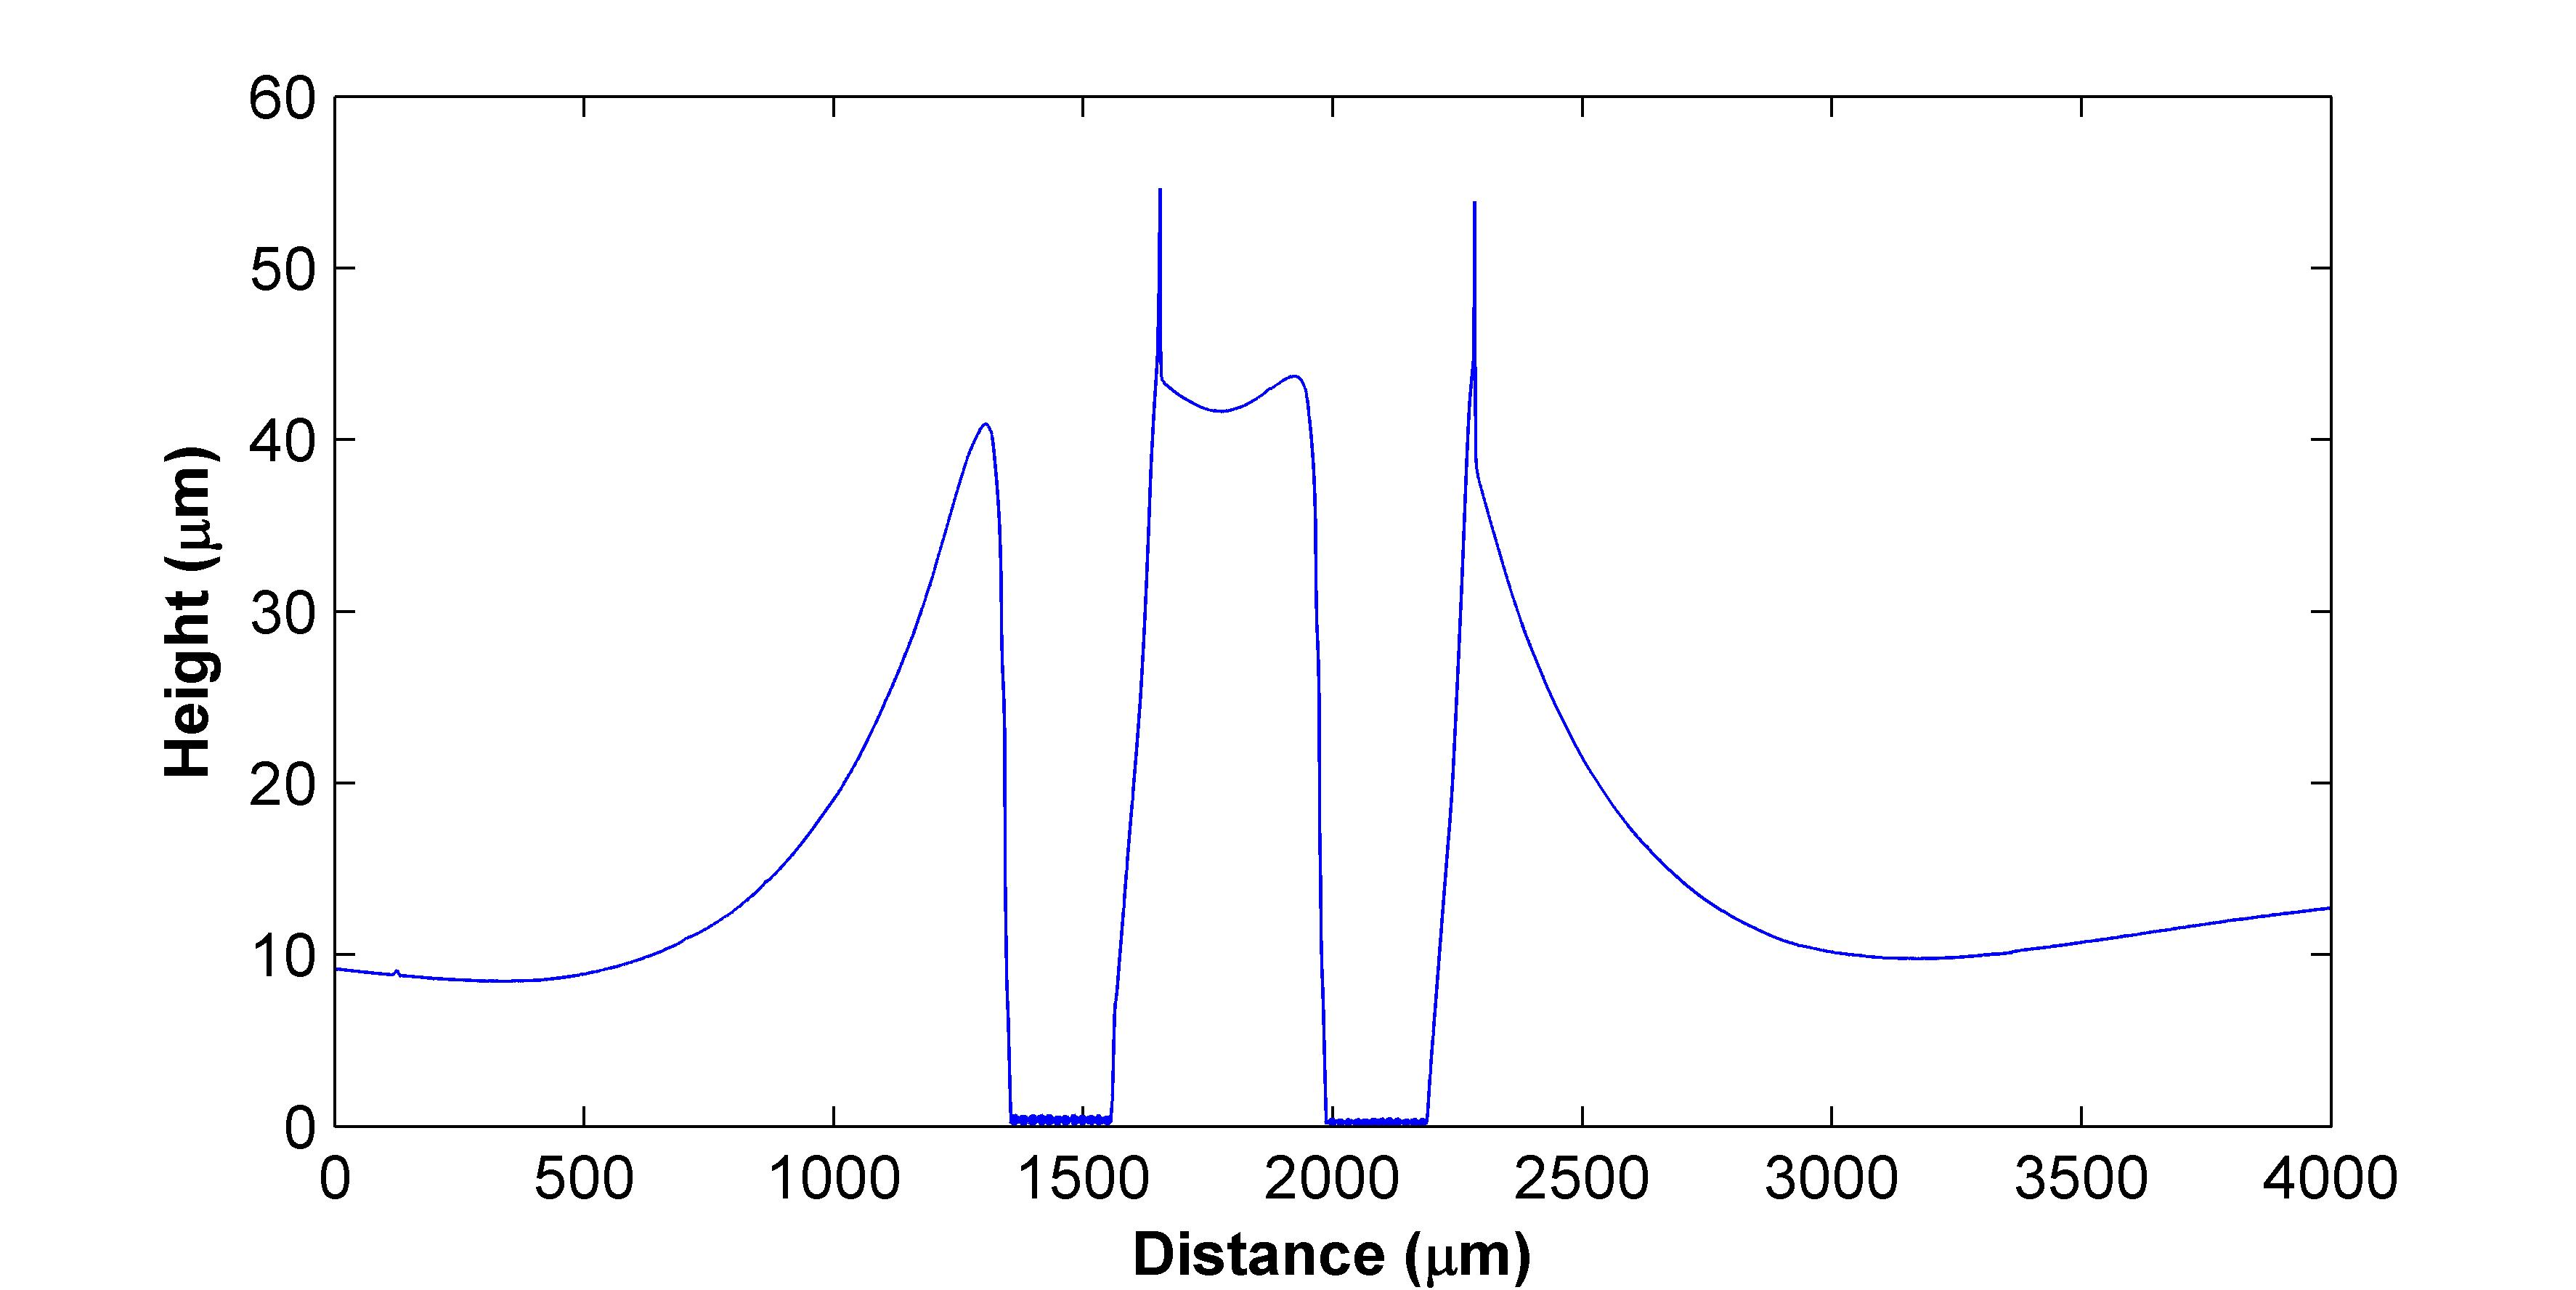
\includegraphics[width=14cm]{chapter2/figures/mw_profile/mw_profile.jpg}
            \label{fig:methods:mwProfile}
            \caption[Representative profile of a PDMS with microwells manufactured by spinning liquid pre-polymer on a SU-8 mold]{\textbf{PDMS sheets with microwells manufactured by pouring liquid pre-polymer on a SU-8 mold were characterized by a an elevated ridge around the cut out shapes.} The measurement was made with a micro-tip profiler on a PDMS sheet with a pair of \(300 \mu m\) microwells. The sharp peaks on the right edges of the microwells are an artefact resulting from the PDMS being dragged up by the profiler tip.}
        \end{figure}


        \subsection{PDMS extraction}
        PDMS extraction was required to avoid cytotoxicity associated with oligomer leaching in certain devices, namely the ones used in chapters \ref{chap:devicesAndFlow} and \ref{chap:microculturePulses}. The extraction protocol was based on \cite{millet2007microfluidic}. Engraved PDMS blocks or cut out thin films were transferred into a Duran bottle and subjected to the following solvent immersion steps (hours): Pentane (16, Sigma, 158941-2.5L), Pentane (8), Xylenes (1, Sigma, 247642-2.5L), Xylenes (16), Xylenes (8), IPA (1, Fischer Chemical, P/7507/PB17), IPA (16), IPA (8), DDW (8). After the solvent immersion the devices were placed in a 120\degree C oven for at least 56 hours. This was required to completely remove the solvent chemicals which are themselves very toxic.


    \section{Bonding techniques}
    \label{sec:methods:bonding}
    \subsection{Plasma bonding}
        Oxygen plasma activation creates hydroxyl (OH\textsuperscript{-}) groups on surfaces. Where silicon (Si) atoms are present as in glass and PDMS, the OH\textsuperscript{-} groups will covalently bind to them.

        PDMS surfaces were pre-cleaned \(3\times\) with scotch tape. Glass surfaces were pre-treated in the same way that they were prepared for surface chemistry (section \ref{sec:methods:surface}). The parts were placed in a plasma oven with the active surfaces facing up. The parts were oxygen (N\textsubscript{2} free) plasma-activated at \(50W\) and \(200 mTorr\) for 30 seconds. Activated parts were removed from the oven and bonded within 2 minutes, before the OH\textsuperscript{-} groups could be passivated by moisture content in the air. Where careful alignment between surfaces was needed, (two layer microwell devices, section \ref{sec:devices:microcultures}) a low magnification microscope (dissection-scope) was used. Bonded devices were finally transferred to a 120\degree C oven where they were kept for 2 hours to facilitate the covalent bonding and to render them sterile.

        \subsection{Double sided silicone tape}
        Silicone-based adhesive transfer tapes of thickness \(50\mu m\) or \(125\mu m\) (3M, 91022 or 96042, respectively) were used. The tapes are provided with a white polyethylene terephthalate (PET) primary release liner, and were backed onto an optically clear Polyester (PE) secondary release liner (also 3M). Geometries were designed using CAD software (Autodesk Inventor Professional) and exported in .dxf format to a plotter cutter (Silhouette Cameo, Graphtec) which excised them from the liner-tape-liner stack. Devices were assembled starting with a bulk PDMS layer. PDMS was mixed, cast and cured as described previously (section \ref{sec:methods:softLitho}) in a petri dish with no feature mould so that a smooth flat surface was formed for the tape to adhere to. The secondary release layer was removed from the tape and the exposed silicon adhesive brought into contact with the PDMS. Flow connections were punched using a \(0.5mm\) biopsy punch (ProSciTech) and cleaned of debris by pushing DDW through them. The primary release liner was then removed and the second adhesive surface brought into contact with either a glass coverslip or an MEA. Initial contact was performed at room temperature.

        \begin{figure}[h]
            \centering
            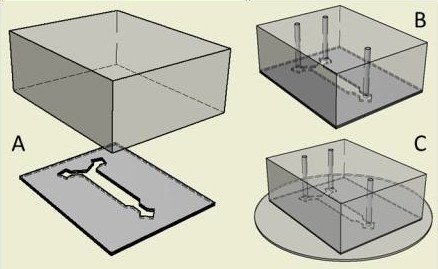
\includegraphics[scale=0.7]{chapter2/figures/tapeBonding/tapeBonding.jpg}
            \caption[Illustration of tape-based device fabrication process]{\textbf{Illustration of tape-based device fabrication process.} The secondary liner is removed and the tape flipped over to adhere to the PDMS (A). Once adhered, access ports are cut with a biopsy punch (B), before the primary liner is removed and the device attached to glass (C). Figure was adapted from \cite{johnstoneThesis} with permission.}
            \label{fig:methods:tapeBonding}
        \end{figure}
        \label{sec:methods:tape}

        \subsection{Pre-polymer bonding}
        The \(19mm\) coverslips were cleaned as in section \ref{sec:methods:surface} and the PDMS channels were produced as in section \ref{sec:methods:softLitho}. A \(22mm\) diameter coverslip was placed on the spin-coater. A few drops of PDMS curing pre-polymer were pipetted onto the glass and the coverslip was then spun at 2000 RPM for 30 seconds, leaving a \(20\mu m\) layer of pre-polymer. With the \(22mm\) coverslip vacuum clamped in place, the PDMS channel was brought into contact with the pre-polymer layer for a few seconds and then lifted off. This coated the base surface of the PDMS with catalyst while leaving the channel unaffected. The PDMS was then placed in contact with the \(19mm\) glass coverslip. The device was finally placed in a 120\degree C for 2 hours for curing and sterilization.


        \begin{figure}[h]
            \centering
            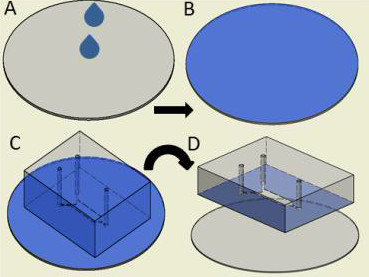
\includegraphics[scale=0.7]{chapter2/figures/glueBonding/glueBonding.jpg}
            \caption[Illustration of the pre-polymer bonding process]{\textbf{Illustration of the pre-polymer bonding process.}  Catalyst is pipetted onto a \(22mm\) coverslip (A) and spun to a uniform thickness (B). PDMS channel is stamped on the catalyst (C) and transferred to a \(19mm\) coverslip (D) before thermal curing of the catalyst. Figure was adapted from \cite{johnstoneThesis} with permission.}
            \label{fig:methods:glueBonding}
        \end{figure}


    \section{Surface coating}
    \label{sec:methods:surface}
        \subsection{PLL coating}
        To coat open surfaces (e.g., MEAs in chapter \ref{chap:activity}) they were incubated (37\degree C, 90\% humidity) overnight with 0.5 ml drop of 0.01\% PLL solution (Sigma, P4707-50ML) in the centre. The next morning, the PLL was removed and the surfaces were washed with DDW \(2-3\times\). In each washing step the surfaces were left immersed in the DDW for a few minutes to allow dissolution of free PLL oligomers. Finally, the surfaces were left uncovered in the sterile hood for at least 2 hours to dry. In cases where `surface-then-bond' device assembly approach was used (used in section \ref{sec:devices:bonding}), a flow layer excised from a double sided silicone tape and already joined to a PDMS bulk (section \ref{sec:methods:tape}) was glued to the surface at this point.

        To coat the internal surface of a device after it had been assembled, i.e., `bond-then-surface' (used throughout most of section \ref{sec:devices:protocolDev}), the assembled devices were flushed with PLL by placing a \(200\mu l\) drop on top and pulling through with a \(1ml\) plastic syringe. The devices were incubated as above overnight in a \(90mm\) petri dish with an accompanying smaller dish containing DDW to reduce evaporation. The next morning, all PLL was removed by pulling with a \(1ml\) syringe and devices were flushed twice with growth media (see section \ref{sec:methods:culture}).

         Both surface-then-bond and bond-then surface devices were finally immersed in \(2.5-3 ml\) of growth media. The immersion ideally occurred the night before the cell seeding because it induced a slow bubble formation within the channel due to air escaping the PDMS as it became wetted. Thus further and final flushing was performed the next day to remove the trapped air bubbles.

        \subsection{PEI coating}
        Following chapter \ref{chap:devicesAndFlow} we switched to using exclusively PEI for surface coating as it is known to produce better adhesion as compared to PLL on some surfaces \cite{wiertz2010regulation}. Indeed we found that using PEI gave rise to more consistent preparations. PEI required adherence to a strict protocol to make sure that no soluble monomers, which are very toxic, are present.

        To prepare the coating solution, 50\% PEI (Sigma, P3143-100ML) was diluted \(500\times\) in DDW (sonication was required for complete dissolution) and sterile filtered. To coat open surfaces a \(0.5ml\) drop of the coating solution was pipetted on the surface center and left in room temperature for 2 hours. The surfaces were then washed with DDW thrice whereby in the final washing step they were immersed in DDW for 2 hours. Finally they were left in the hood to dry for at least a few hours, typically overnight. At this point, tape and PDMS layers were joined to the surface to complete the assembly of the device. In the case of MEAs a glass cylinder was glued to hold the immersion media (see image in figure \ref{fig:pulses:circularIllustration}). The final pre-seeding immersion was performed as described above for the PLL but with \(4ml\) of media to ensure enough supply for `self media' flow experiments (see section \ref{sec:crossFlow:intro}).

 \section{Seeding and maintaining of Neuronal cultures}
 We used growth media based on Neurobasal (Invitrogen, 21103-049) supplemented with B27 (Invitrogen, 17504-044) and and \(0.5mM\) L-Glutamine  (Sigma, G7513). Harvesting of primary hippocampal and cortical cells seeding solutions was as follows: the entire cortices of E-18 pregnant rat embryos were removed. Cortices were then subjected to further dissection for precise removal of the meninges and excision of the hippocampi. Hippocampi and 2-3 cortices were then each placed in a dish with \(2ml\) Hank's solution with 0.1\% trypsin and 0.005\% DNAse (Sigma, D5025-15KU) for 20 minutes following which 0.05\% trypsin inhibitor (Sigma, T9003) was added to de-activate the trypsin. The tissue was then transferred to a falcon tube, washed once and suspended in \(1.5ml\) growth media with 0.005\% DNAse. Next, the tissue was triturated with a flame polished glass pasteur until the cells were fully in suspension. The cells were then centrifuged and re-suspended again in \(1.5ml\) growth media. Finally, the cells were counted and diluted or concentrated as necessary (by centrifuging and re-suspending) to the final required seeding density.

 Open MEAs were seeded by placing a \(0.5ml\) drop of cortical seeding solution in the centre of the sample. The cells were allowed to settle for 30 minutes in the incubator, after which the media was topped up to \(1ml\). This is relevant to all the samples used in chapter \ref{chap:activity}.

 Devices were seeded by injecting \(1-3\mu l\) of hippocampal seeding solution into the outlet port using a gel-loading tip. In all microculture devices as well as devices used for flow with self media (see section \ref{sec:crossFlow:intro}) external support cultures were seeded as well. These comprised further cortical cells plated on the exposed coverslip or MEA surface around the PDMS device at a volume density of \(50-100 \frac{cells}{\mu l}\). In the case of microculture devices, a further flushing step was employed the following day to remove excess cells residing outside the microwell. The microculture devices in section \ref{sec:devices:microcultures}, where the surface outside the microwells was cell adhesive, required aggressive flushing which was performed by pulling media through with \(1ml\) syringe. This action selectively removed cells from the top of the PDMS sheet and not from the within the microwell by virtue of the shear protection that it confers. However, in some cases a noticeable amount of cells were removed also from the wells. In contrast, the microculture devices in chapter \ref{chap:microculturePulses}, where the surface outside the microwells was not cell adhesive, were conducive to gentle flushing which was performed by pushing \(20\mu l\) media through the channel using a syringe driver at a rate of \(50-100\frac{\mu l}{min}\). In this way, no cells were removed from the microwells.

 After plating, devices were placed in a humidified 5\% CO\textsubscript{2} incubator. Media in device preparations was changed by replacing approximately a third of the immersion media. Media change was normally performed twice a week. However, for samples in chapter \ref{chap:microculturePulses} the media was changed only 3 times to maximize its saturation with conditioning factors towards its subsequent use for self media flow.


         \label{sec:methods:culture}

\section{MEA recording and stimulation}
Multi electrode array recordings were performed with commercial MEAs (Multi Channel Systems, 60MEA200/30-Ti or 60HDMEA30/10iR-ITO). Electrical activity was recorded with a 60-channel USB amplifier system (USB-MEA60-Inv, Multi Channel Systems) fitted in the environmental chamber (37\degree C) and using MCRack recording software (Multi Channel Systems) with 2nd order Butterworth band pass filtering (\(200-3000Hz\)).

\label{sec:methods:MEARecording}

\subsection{Spike detection and noise removal}
Preliminary spike detection was performed in real time using MC Rack whereby only \(20 ms\) windows around threshold crossings were stored. These thresholds were channel specific and were typically automatically set to \(-5.5\) standard deviations of the channel baseline noise. This definition catered for most extracellular spike shapes where the peak deflection was negative. In the minority of cases, where most spikes in the channel had a positive peak deflection (sometimes termed inverted spikes) we set the threshold to \(+5.5\). A second filtering step utilized the wavelet packet decomposition method and software package from \cite{hulata2002method} to exclude noise. In essence this is based on a wavelet function optimized to best represent noise features and so spikes were further excluded by applying a second threshold to the correlation between the spike waveform and the noise wavelet. Examples of this procedure and the effect of the second threshold are provided in figure \ref{fig:methods:matchFilter}.

\begin{figure}[!htb]
\centering
\includegraphics[width=15cm]{chapter2/figures/matchFilter/matchFilterIllustration.jpg}
\caption[Examples of spike detection and shape based artefact removal]{\textbf{A two-step spike detection procedure is effective at excluding spike artefacts.} 3 example windows of filtered electrical data (band pass \(200-3000Hz\)). Initially spike times are determined by crossings of electrical threshold (marked by cyan lines). However, spike waveforms (marked by a color overlay in a \(2ms\) window around crossings) are further subjected to correlation with a wavelet function representative of noise. Thus a second threshold is applied to the correlation to exclude noise-resultant spike waveforms. Application of second threshold is exemplified using two values. Spikes marked by green overlay are ones accepted by both correlation thresholds and those marked in red are excluded by the higher threshold. The higher correlation threshold value (34) was the value used for spike detection throughout this work. The units for the second threshold are arbitrary (the value is derived from an un-normalized correlation function).}

\label{fig:methods:matchFilter}

\end{figure}

We found that the above shape based spike detection procedure was effective at removing some spike artefacts but in many cases they were erroneously retained. Most obvious were cases where, presumably due to external electromagnetic induction, such artefact spikes were elicited simultaneously across many channels, if not all. Such cross channel artefact spiking events were significantly more synchronized than even real neuronal bursts and so could be easily discerned simply by applying a threshold to the summated firing rate plot (where the former types of events were characterized by sharp peaks). Thus a final noise exclusion step was routinely employed where all spikes in a \(5ms\) window around such synchronized artefact spiking events were removed (figure \ref{fig:methods:syncArtefact}).

\begin{figure}[!htb]
\centering
\includegraphics[width=14cm]{chapter2/figures/syncArtefact/syncArtefact.jpg}
\caption[Example for synchrony based spike artefact removal]{\textbf{Synchronized spike artefacts events are easily discerned from actual biological bursting events via their increased synchronicity.} (A-B) A channel raster plot segment and its summation plot at \(1ms\) binning. (C) Filtered electrical data from one of the electrodes showing the detected spikes as red overlays. The rightmost detected spike is an artefact. (D-E) Same raster plot and summation as in A-B after removing the spikes associated with the artefact event. The event was detected by applying a threshold (in this case set to 10 spikes) to B and all spikes in a \(5ms\) window around the threshold crossing were excluded.}

\label{fig:methods:syncArtefact}

\end{figure}

\subsection{Electrical stimulation}
Individual stimulations consisted a rectangular and biphasic \(800 ms\)-long voltage pulses of \(300-900 mV\) were applied to the selected electrodes using either a 2-channel stimulus generator (STG 2002, Multi Channel Systems) or a data acquisition card capable of generating analogue voltage signals (DAQ, National Instruments, SCB-68A). The latter option was used for the plasticity protocol in section \ref{sec:activity:plasticityProtocol} where a complex stimulation sequence including both test pulses and tetanus was required. In this case, custom made Labview software was employed.

\label{sec:methods:stim}


\subsubsection{Automatic detection of responsive channels}
In some cases, the stimulation response data was presented in the form of a response chart which reflects the spatial arrangement of the recording channels and the of response in each is indicated via color coding. The response, in this case, is measured as the average number of spikes recorded in this channel at a time window \(10-210ms\) from the stimulation time (see examples in fig \ref{fig:activity:stimExample}). To make the charts clearer, we sought to exclude channels which were occasionally active during the above observation window by chance, due to ongoing spontaneous activity. Consequently, we employed a procedure where we collected the mean firing rates in the observations windows (i.e., \(10-210ms\) after the stimulation) for all stimulations as well as the mean firing rates in windows that are \(500ms\) distant from any stimulation and therefore represent the ongoing spontaneous activity. A t-test was employed between the above groups of measures and only channels showing significantly higher firing rate in the first window were kept and indicated in the chart. The significance threshold depended on the number of stimulations performed in the specific experiment and was therefore selected purely on the basis of obtaining visually pleasing results.


\subsection{Correlation maps}
To produce correlation maps, i.e., a correlation matrix, channel rasters at \(1ms\) binning were convolved with a gaussian kernel of width \(\sigma=100ms\). The correlation between pair of channels was simply defined as the Pearson correlation coefficient between the respective gaussian smoothed rasters. In some cases, a surrogate correlation map was computed based on the same data but where all the channel rasters were replaced by independent poisson processes with the same firing rate as in the respective channels (i.e., \(\lambda\) set to be the original channel firing rate). This procedure is illustrated in figure \ref{fig:methods:corrIllustration}.

\label{sec:methods:corrMaps}
\begin{figure}[!htb]
    \centering
    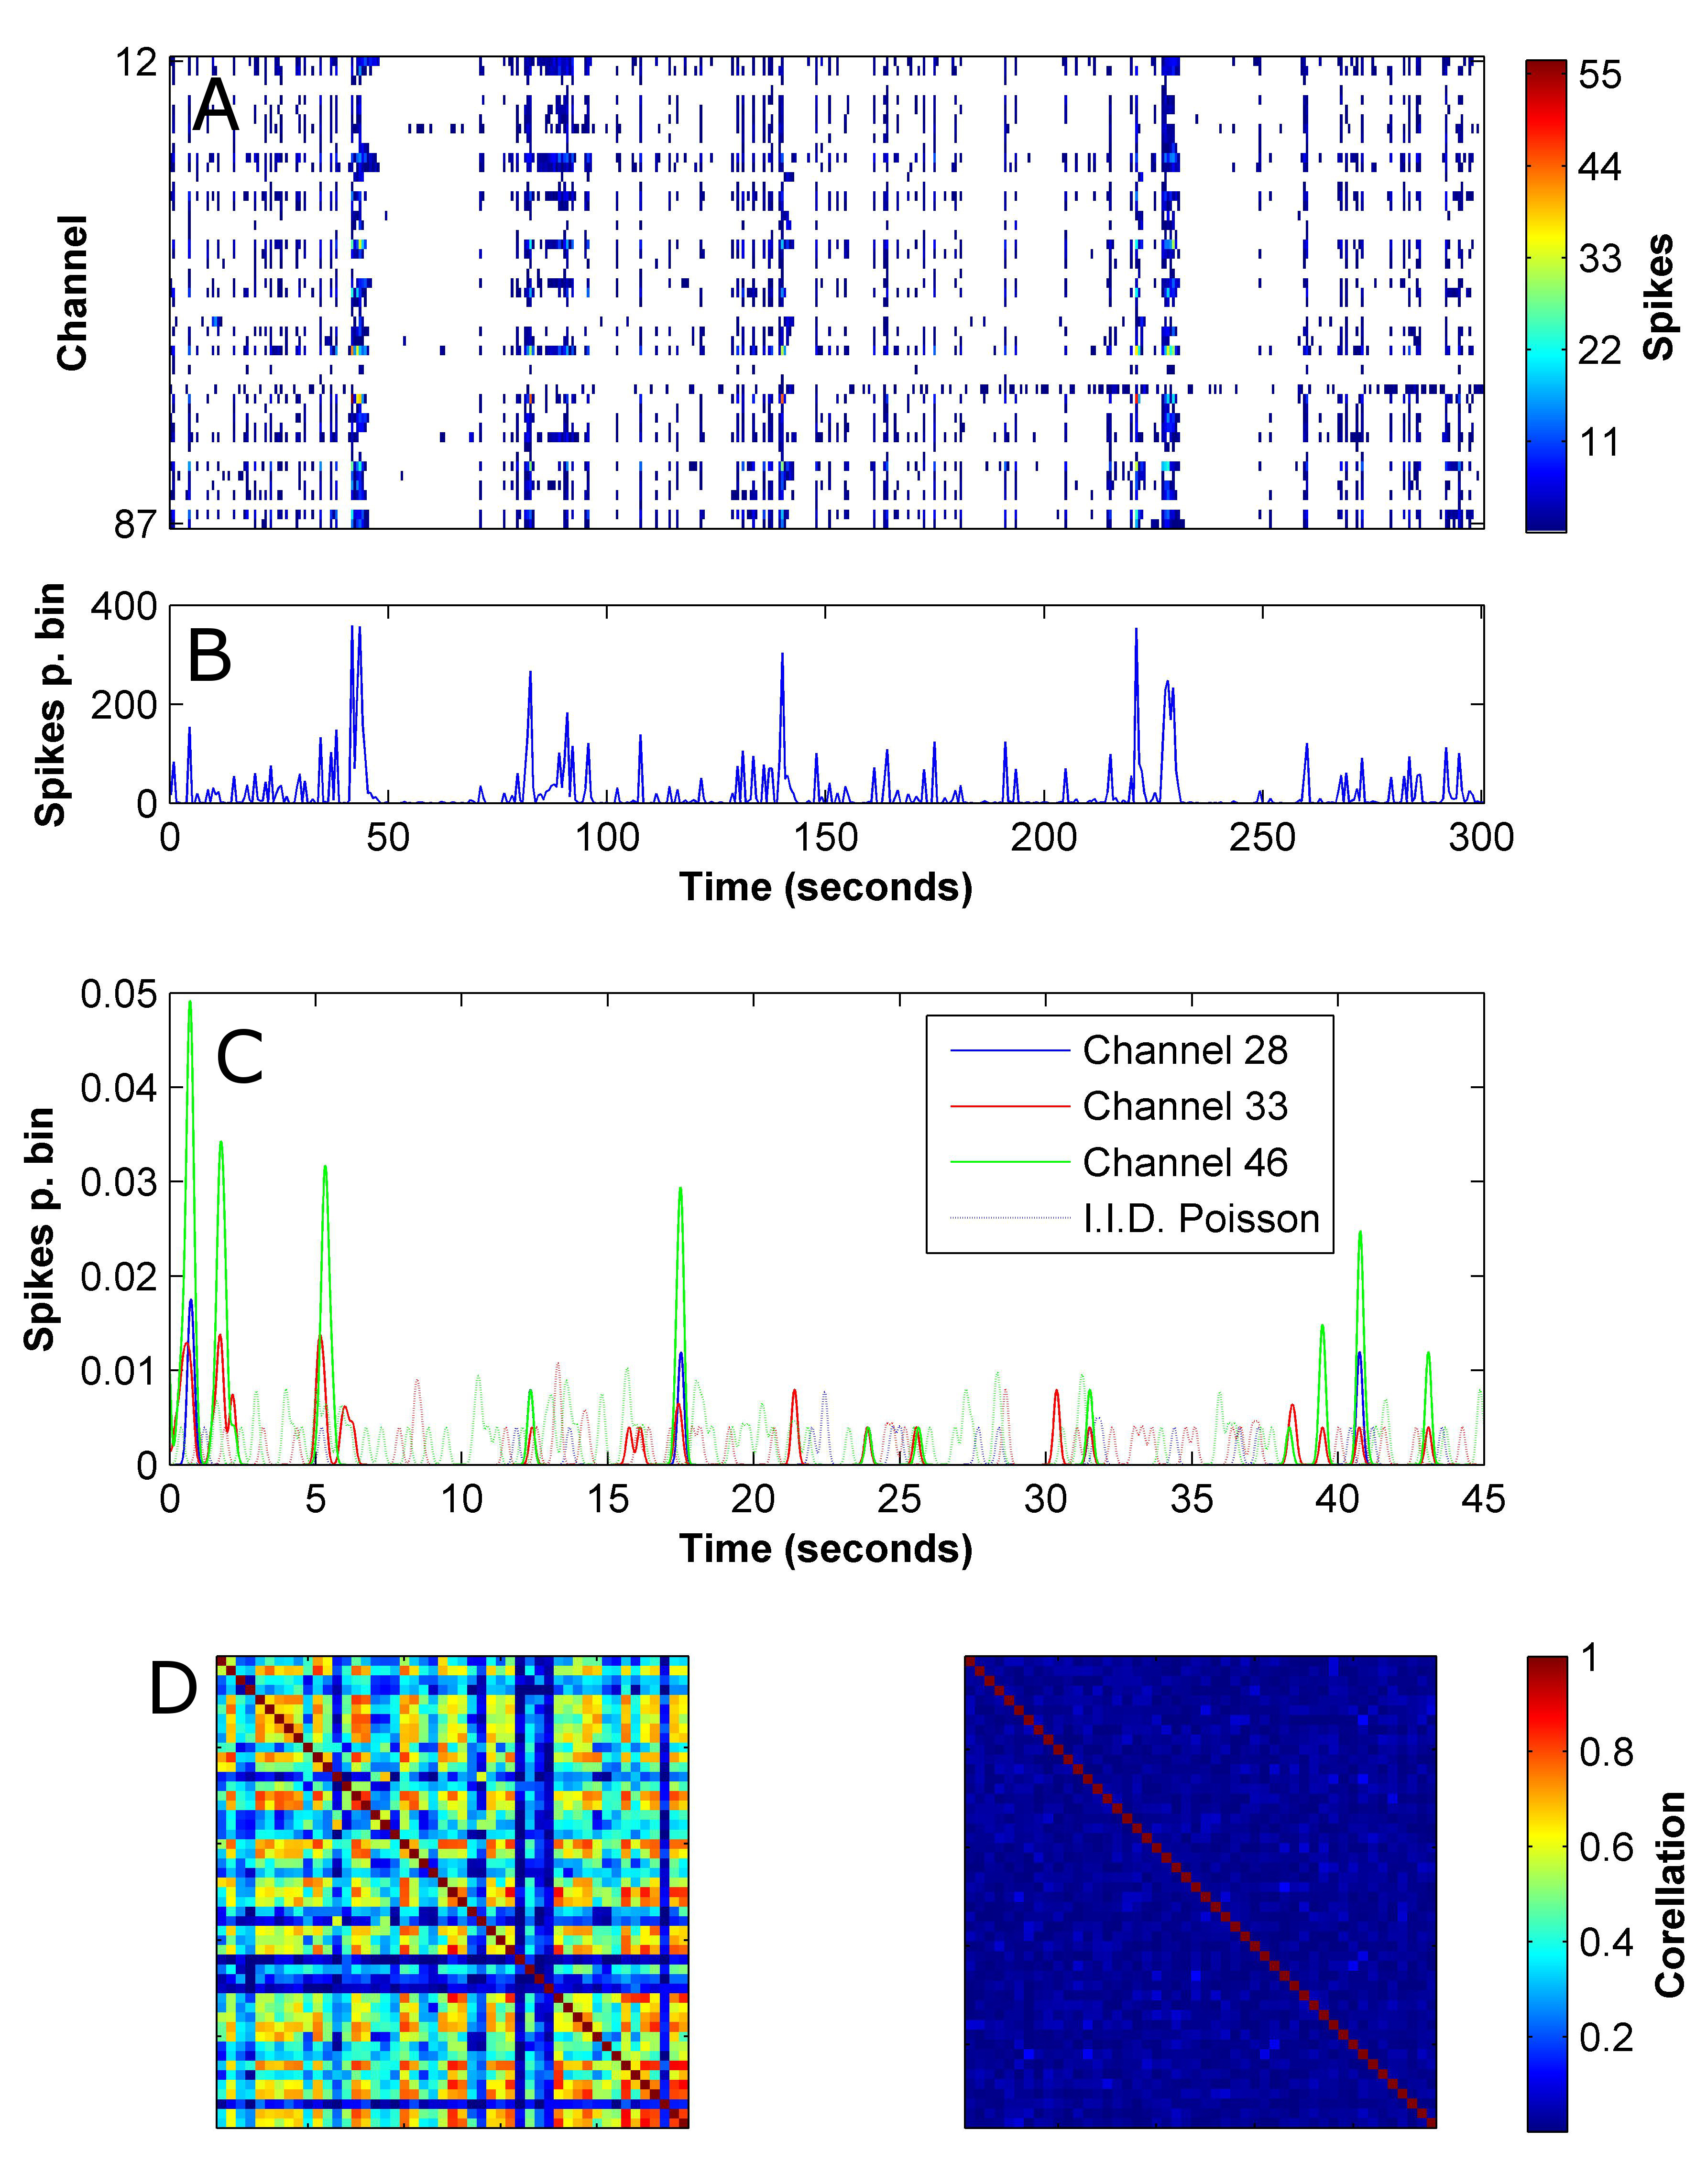
\includegraphics[width=14cm]{chapter2/figures/corrIllustration/corrIllustration.jpg}
    \caption[Computation of correlation maps]{\textbf{Comparison to surrogate maps based on independent poisson raster with firing rates as in the original data highlight the correlations in the data.} (A-B) Channel raster plots and their summation at \(0.6s\) binning. (C) Gaussian smoothed raster plot for 3 channels from the recording shown in A-B. Surrogate smoothed raster plots are shown for the same channels in dotted lines with same color coding. Evidently, the original data is significantly more correlated. (D) Correlation maps for original data (left) and surrogate (right).}
    \label{fig:methods:corrIllustration}
\end{figure}
\subsection{Burst detection}
Bursts are usually detected by applying a threshold to the firing rate plot. In contrast to previous attempts \cite{wagenaar2006extremely,chiappalone2005burst} where the threshold was somewhat arbitrary, we have devised a method to select an informed threshold value that would reflect whether the channels are synchronized or independent. To obtain such a threshold for a given recording we generated surrogate channel raster plots where the spike times were randomly drawn from a Poisson process with a rate parameter (\(\lambda\)) set to be the firing rate of the corresponding channel in the original data. These surrogate raster plots were summated, smoothed with a gaussian kernel with \(\sigma=70ms\) and the threshold was set to be 5 standard deviations above the mean of the resultant signal. Thus, all peaks above this threshold in the smoothed raster plot sum in the original data were defined to be bursts. Bursts that were closer than \(100ms\) were grouped into one whose time was taken to that of the highest peak.

The next stage of the analysis was to find burst limits (start and end). This process utilized two thresholds. One (firing rate threshold) was set, as before, to be 5 standard deviations over the mean of the surrogate smoothed raster plot sum curve. The second (derivative threshold) was set to be just the standard deviation of the derivative of the same surrogate curve. The start and end of a burst were defined as the closest points on the smoothed raster plot sum around the burst peak where the curve dips below the firing rate threshold, where the absolute value of the first derivative is below the derivative threshold and where the second derivative is positive. Since a relatively wide smoothing kernel was required which caused blurring of sharp event boundaries, we finally shifted the start and end points defined by the above criteria towards the peak, by half of the kernel width. The first threshold implements the original intuitive idea whereby the burst is a time window where the summated network activity is elevated as compared to what is anticipated by the surrogate raster plots. The second threshold can be thought of as applying the same intuitive idea but on the derivative. This extra threshold was required because when the boundaries were defined based only on the first one, they were sometimes so close that the final half kernel shifting caused the end time to be earlier than the start. The final threshold was required to make sure that points around troughs are detected and not around burst peaks. Examples of output from this procedure are shown in figure \ref{fig:methods:burstDet}.


\label{sec:methods:burstDetection}
\begin{figure}[!htb]
            \centering
            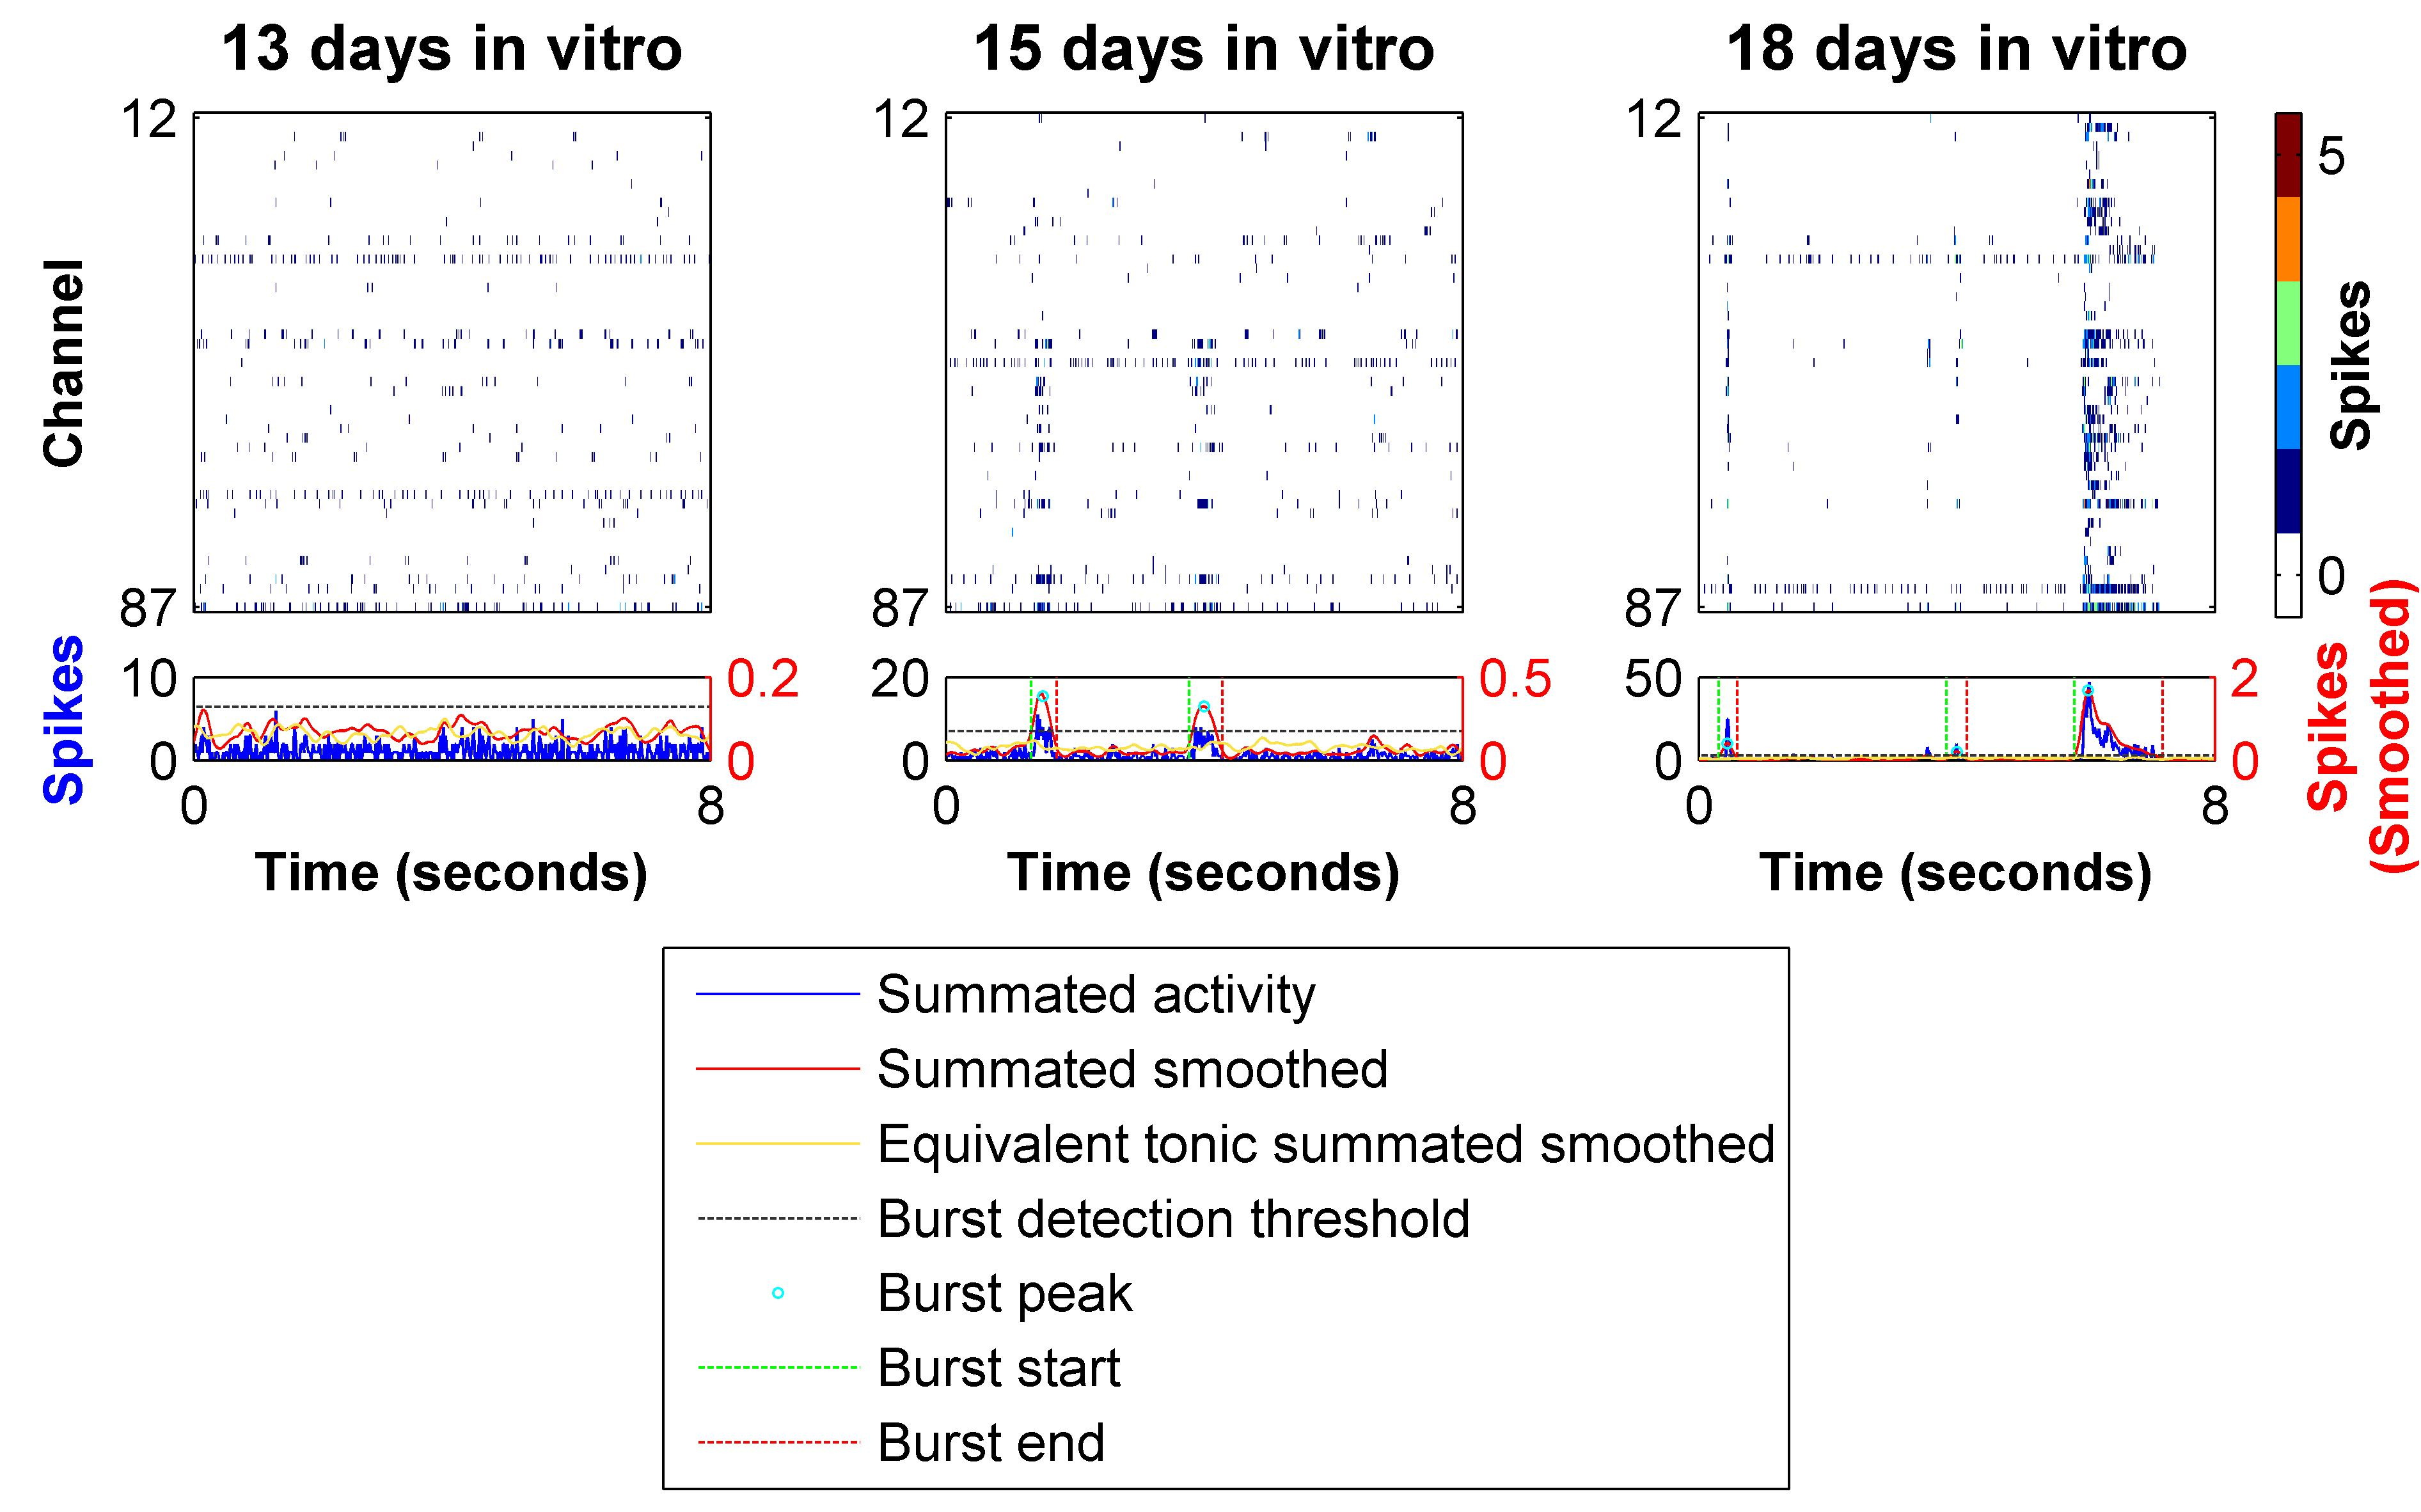
\includegraphics[width=15cm]{chapter2/figures/burstDetection/burstDetExample.jpg}
            \caption[Examples of burst detection output]{\textbf{The burst detection algorithm is sensitive to a range of synchronized burst scales.} Raster plots and their sum from a single cortical mouse culture at different developmental stages are shown. Also shown are derived curves used for the burst detection procedure and the outputs of the algorithm (i.e., burst peak, start and end points). See text for further details.}
            \label{fig:methods:burstDet}
          \end{figure}

\subsection{Functional connectivity analysis}
Computation of the functional connectivity (FC) measure completely followed the concepts introduced in \cite{le2007conditional} and where the ideas are explained in greater detail. Functional connectivity is defined between pairs of channels. The computation was performed directly on the channel raster plots at \(1ms\) binning without any smoothing and FC was essentially defined as the cross correlation between the plots normalized to the number of spikes in the first channel: \[FC_{i,j}[\tau]=\frac{\sum{t}^{}X_i[t]\cdot X_j[t-\tau]}{N_i},\] where \(X_i\), \(X_j\) are the channel raster plots, \(N_i\) is the number of spikes in channel \(i\) and the computation was performed for \(0\le \tau \le 500ms\). Thus the FC measure reflects the probability of observing a spike in channel \(j\) at time \(\tau\) given an occurrence of a spike in channel \(i\) at time \(0ms\). When the FC curve is not flat (i.e., it contains a peak) this indicates a true association between the channels. To characterize the FC curve it was further fitted to the following function, which essentially describes a hump of height \(M\) at a distance \(T\) from the y-axis with a baseline as offset \(o\) from the abscissa: \[FC_{fit}[\tau]=\frac{M}{1+\left(\frac{\tau-T}{w}\right)^{2}}+o.\]
A functional connection was considered to be present if, in the above fit, \(M>5\cdot o\), which indicates a significant peak. The fit also had to be rejected if it resulted in parameters with extreme values and so additional conditions were imposed: \(10<w<250\) and \(T<250\). FC was calculated only when both channels had at least 200 spikes as otherwise the generated curve was too noisy to analyze meaningfully.

Figure \ref{fig:methods:FC} shows example of functional connectivity curves and their respective fits to demonstrate that this measure was applied to our data with meaningful results.

We would like to emphasize that the parameter \(M\) above reflects the strength of the connection (i.e., the probability of observing paired spikes in the analyzed channels) and \(T\) is the characteristic time delay between such spikes. In this Ph.D work, we used two types of preparations, macrocultures and microcultures. In the case of macrocultures, the recordings sites were spread over a significantly larger area of tissue and this difference was indeed reflected in the values obtained for the parameter \(T\). In the case of macrocultures, values in the range of \(0-106ms\) were observed and 60\% of the values were smaller than \(1ms\). In the case of microcultures, a smaller range of \(0-20ms\) was observed and 96\%(!) of the values were smaller than \(1 ms\). These differences might reflect simply the proximity electrode pairs in the microculture recordings but it might also indicate a higher degree of coupling between the neurons in such preparations.

\begin{figure}[h]
\centering
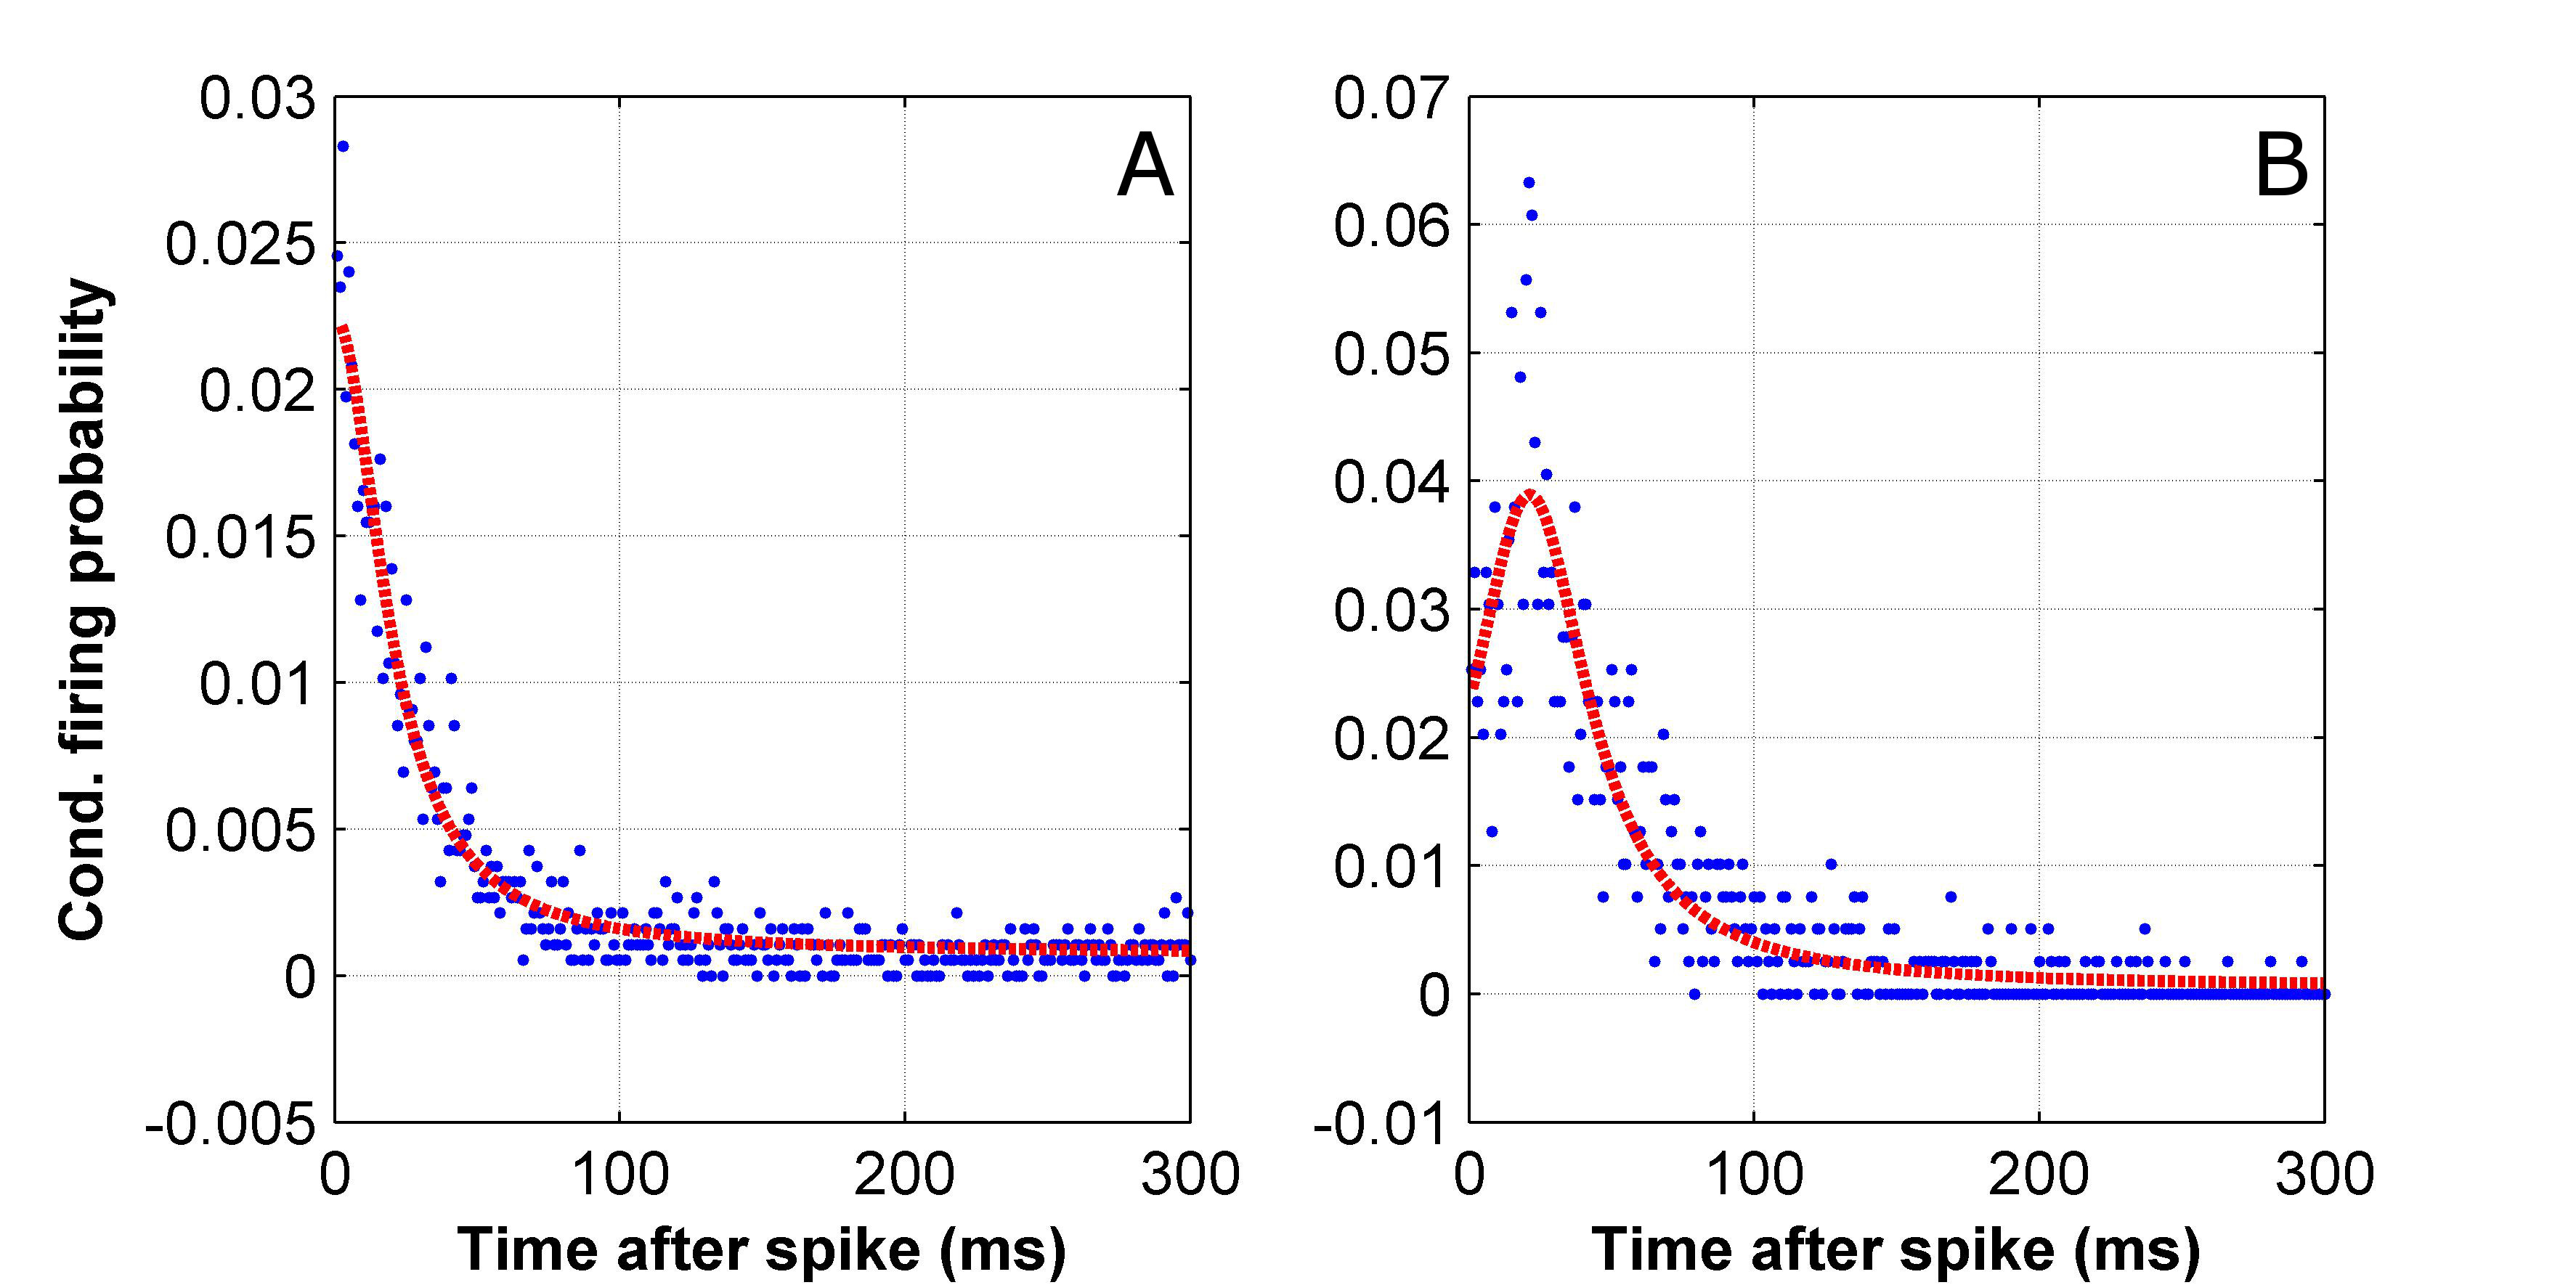
\includegraphics[width=15cm]{chapter2/figures/FCDemonstration/FCDemonstration.jpg}
\caption[Examples of functional connectivity curves]{\textbf{Functional connectivity curves exhibit localized peaks that reflect the coupling between neurons recorded at the analyzed pair of electrodes.} 2 FC curves are shown from a spontaneous activity recording in a mouse culture grown on a standard \(8\times 8\) MEA. (A) A FC curve with a peak at \(\approx 0ms\) (\(T=10\times 10^{-5}ms\)). This type of functional connection might represent a neuron pair that is strongly coupled or where both neurons are driven by similar synaptic input. (B) A FC curve with \(T=21ms\). This functional connection represents a characteristic propagation delay in the network.}

\label{fig:methods:FC}
\end{figure}
\label{sec:methods:FC}

\section{Conditioned media production}
In section \ref{sec:devices:viabilityAssay} we explored the link between the culture's viability under flow and the conditioning levels of the flow media. This required a standardized conditioning scale. Here we describe the production of such conditioned media and the definition of the standardized scale. Cortical cells were used for the purpose of media conditioning as they are available at larger quantities. These were seeded into T-12 flasks, \(3\times 10^6\) cells per flask, in a final volume of \(5 ml\). Flasks were kept in the incubator without changing the media until reaching the desired conditioning level at which point the media was collected and used for flow experiments. Conditioning level was calculated by: \(round\left(\frac{12\cdot DIV}{35}\right)\) where \(DIV\) is the number of days from plating. According to this scale, for every \(\approx\) 3 days in the flasks, the media accumulates 1 conditioning unit.
    \label{sec:methods:cond}



\section{Flow experiments}
\label{sec:methods:flow}
Flow control was performed with a pressure-driven microfluidics flow control system (Eleveflow, France) comprising a 4-channel pressure controller (\(0-200 mbar\) gauge pressure range, Elveflow, OBI) and 4 matching thermal mass flow sensors (\(0-7 \frac{\mu l}{min}\) sensing range, Elveflow, MFS2). The apparatus was controlled with the Elveflow software interface (SI2.6.1). The organization of this modern flow control system is illustrated in figure \ref{fig:methods:schematics}. The pressure controller uses fast piezoelectric valves to introduce or vent gas from reservoirs holding the flow media. This control method supports rapid pressure changes with a response time in the order of \(80ms\). We used a 5\% CO\textsubscript{2}/air gas supply to the pressure controller to keep the media CO\textsubscript{2} saturated. The pressure drives the media out of the reservoirs through tubing which are inline with the flow sensors. A PID control loop implemented in software utilizes the flow sensor data to control the flow rates. The flow PID parameters are accessible through the software and were used to control the flow responsiveness.

       \begin{figure}[!htb]
            \centering
            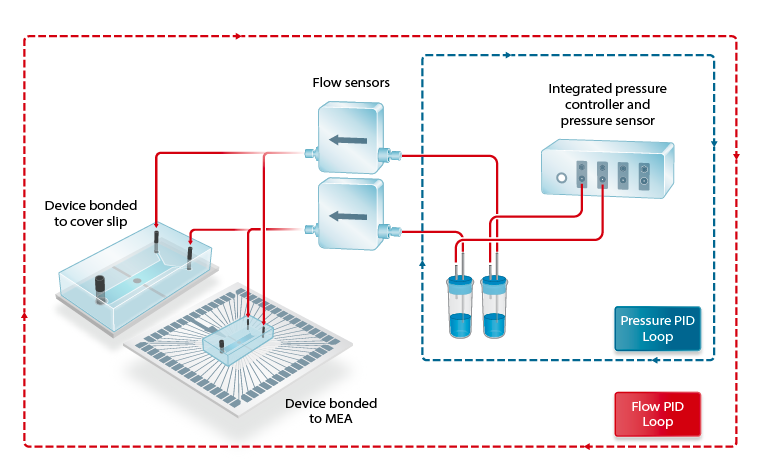
\includegraphics[width=14cm]{chapter2/figures/Schematics/schematics.png}
            \caption[Illustration of flow system]{\textbf{Illustration of flow system.} Pressure in media reservoirs is directly controlled to induce flow which is monitored via inline flow sensors. The control in the system is implemented via nested PID. The user defines the set value of the flow PID which utilizes the set value of the pressure PID.}
            \label{fig:methods:schematics}

        \end{figure}


We used polyether ether ketone (PEEK) tubing (\(360 \mu m\) OD \(150-250 \mu m\) ID, VICI, TPK.106, JR-T-5608-M3 or JR-T-5610-M3)
for the flow lines directly connected to the reservoirs. PEEK was selected on the basis of its low gas permeability and was expected to retain the CO\textsubscript{2} saturation of the media as it flows out of the reservoirs. The PEEK tubing entered a custom made environmental chamber heated to \(37\degree C\) with a 5\% CO\textsuperscript{2} atmosphere (figure \ref{fig:app:chamber}) through a small side hole. Inside the chamber, the PEEK lines were extended by flexible PTFE tubing with a larger ID of \(500\mu m\) which finally plugged into the device via a stainless steel \(1/32''\) needle. All PTFE lines inside the environmental chamber contained inline bubble traps which essentially comprised a PDMS block with a large internal cavity. Air arriving into the bubble trap cavity tended to float up to the upper PDMS surface and did not proceed with the flow. The location of the bubble traps along the flow line was as proximal as possible to the device inlets to minimize the chance of air bubbles forming in the intermediate flow line section. The total tubing volume inside the environmental chamber was 3 times larger than outside. This was purposefully designed to allow the media to reabsorb any CO\textsuperscript{2} lost during the travel in the ambient air from the reservoir to the chamber and heat up to \(37\degree C\). Each flow experiment was initiated by flushing the system with IPA, DDW and finally with the flow media. To connect a flow line to a device port its flow rate was set to \(1\frac{\mu l}{min}\) and it was plugged in only after an obvious drop was formed at the tip of the connector needle to assure that no air was introduced during the connection process. The inlets were always connected prior to the outlet because the latter flow line was loaded with fresh media which should not be allowed to reach the cells. The elasticity of the PDMS was normally enough to create a seal around the connector needle to prevent leaks. However, it should be noted that such leaks from the ports were the most common type experiment failure. Such leaks from the ports or due to failure of the PDMS-surface bond were detected by monitoring the flow rate in the outlet channel to assure that all the flow in the inlets is accounted for (i.e., outlet flow rate is sum of inlet rates).

In cases where flow experiments were performed on coverslip based devices (relevant for section \ref{sec:devices:viabilityAssay}) up to 3 devices could be placed under flow simultaneously using separate flow channels (figure \ref{fig:app:3Devices}). Outlets were combined into a single flow line using a PDMS junction or a ring connector. In the case of flow experiments that utilized self media (chapters \ref{chap:activityAndFlow} and \ref{chap:microculturePulses}) the sample had to be drained of its immersion media so as to transfer it to the flow system's media reservoirs. This was performed after the sample had been placed in the environmental chamber. In this case the sample had to be left with a drop of self media on top to prevent dehydration. After all the device ports were connected (2 or 3) the flow rates could were either set to a steady value (i.e., in the case of the steady flow experiments in chapters \ref{chap:devicesAndFlow} and \ref{chap:activityAndFlow}) or a more complex flow sequence was initiated (chapter \ref{chap:microculturePulses}). Pulsing experiments were controlled by a custom made Labview program which allowed personalized design of chemical and electrical stimulation sequences and communicated with the flow controller and the stimulator (see section \ref{sec:methods:stim}) via TTL pulses.






 \subsection{Viability analysis}
 To quantify the viability of the cultures under flow (section \ref{sec:devices:viabilityAssay}) the flow media was supplemented with \(2.5\frac{\mu g}{ml}\) Propidium Iodide. Dead cells leave behind exposed particles of condensed DNA appearing as fluorescent dots under Propidium Iodide staining. Consecutive fluorescent images of the same culture region in the device were taken every 1-2 hours. Bright field image of same region was also taken at the beginning of the flow session. Images were taken with a CCD camera (QuantEM 512SC, Photometrics or Grasshopper 2, PointGrey) mounted on a wide field fluorescence microscope (Brunel SP-99) and a TRITC ET filter set (Chroma). The number of dead cells in each image was counted automatically using ImageJ by thresholding the fluorescence image and counting the number of separate particles. The number of live cells was counted manually from inspection of the bright field image.
The proportion of live cells in each image was finally calculated as: \[\text{Proportion live cells} (i)=\frac{live(1)-(dead(i)-dead(1))}{live(1)},\] where \(live(1)\) is the number of live cells in initial bright field image and \(dead(i)\) is the dead cell count in image \(i\) of the time lapse.

 \begin{figure}[h]
     \centering
     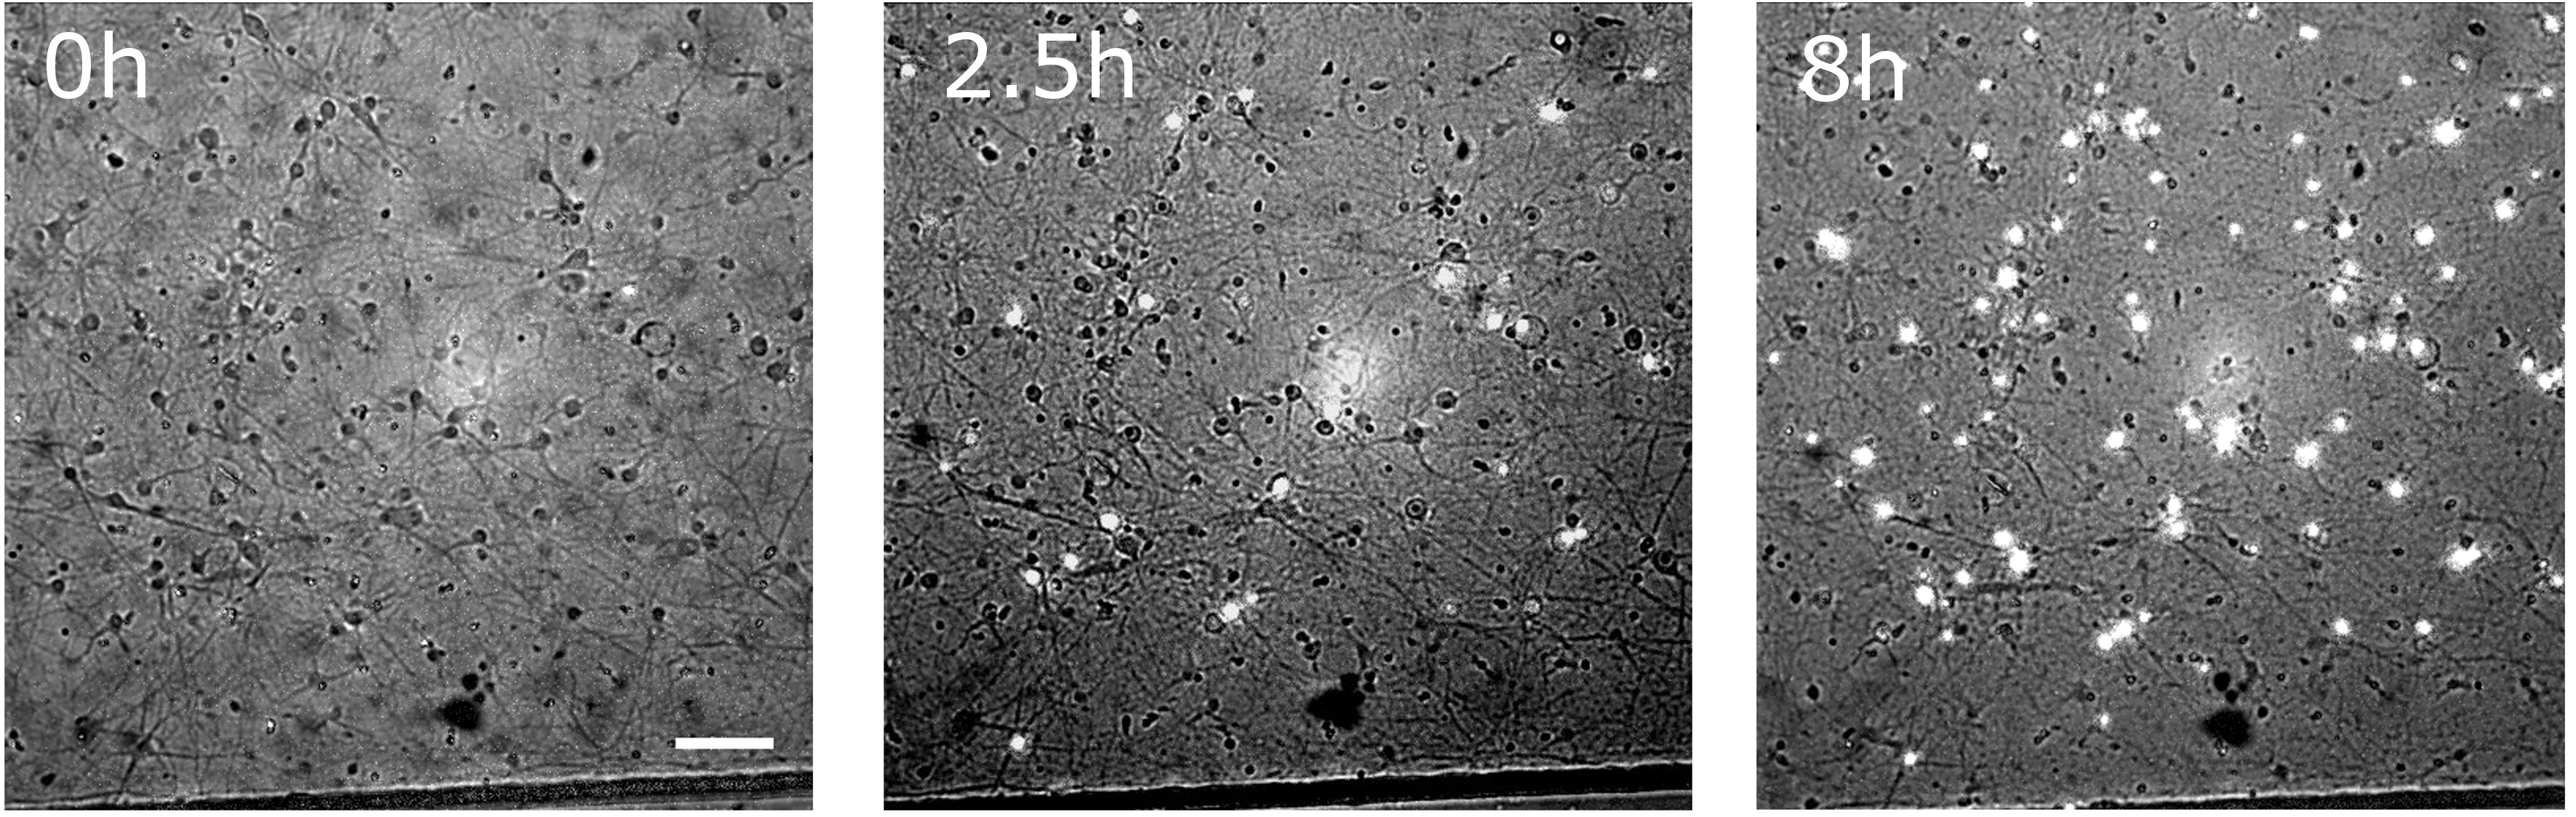
\includegraphics[width=15cm]{chapter2/figures/PIAssayIllustration/PIAssay.jpg}
     \caption[Example fluorescence images of Propidium Iodide staining under flow]{\textbf{Dead cells appear as fluorescent dots under flow with Propidium Iodide supplemented media.} Overlays of fluorescent (TRITC filter set) and bright field images of hippocampal cultures under flow with Propidium Iodide supplemented media. Fluorescent dots were automatically counted using ImageJ. Scale bar is \(100\mu m\) long and is consistent across all images.}
     \label{fig:methods:PIAssay}

 \end{figure}

 \section{Immunofluorescence}
Device samples were washed in a phosphate buffered solution (PBS) by applying a drop on top and pulling through with a \(1ml\) syringe. This protocol was applied specifically in relatively deep microwell devices (\(120\mu m\), section \ref{sec:pulses:microcultures}). The shear protection conferred by these deep microwells prevented the microcultures from being washed away despite the relatively aggressive washing method. All consecutive washing steps in this protocol were applied in the same manner. The sample was fixated with a 4\% paraformaldehyde solution in PBS which also contained 4\% sucrose, \(20mM\) NaOH and \(5mM\) MgCl and pH corrected to 7.4. Next they were washed \(3\times\) with \(10mM\) Glycine in PBS and permeabilized by incubating in \(10mMm\) Glycine and 0.1\% Triton in PBS for 30 minutes.  As a next step they were washed with 0.1\% Triton in PBS and finally blocked through incubation in 3\% BSA for 1 hour. After the blocking, They were  incubated in primary antibodies (see below, 1:250 dilution) and 3\% BSA in PBS overnight at \(4\degree C\). The next day, the samples were washed \(3\times\) with 0.1\% Triton in PBS and incubated in secondary antibodies (see below, 1:500 dilution) and 3\% BSA in PBS. Finally, samples were washed again \(3\times\) in 0.1\% Triton in PBS and incubated in \(0.01 \frac{\mu g}{ml}\) DAPI in PBS for 5 minutes following which they were washed in PBS and imaged using a fluorescent microscope (Nikkon Eclipse Ti) and an EMCCD camera. To detect glial cells, goat anti-glial fibrillary acidic protein monoclonal antibody was used (GFAP, Abcam, ab53554). Neurons were detected using Rabbit Anti-\textbeta III-Tubulin, (Abcam, ab78078). The corresponding secondary antibodies were Alexa Fluor 647 chicken anti-goat (Life Technologies, A21469, imaged with CY5 filter set by Chroma) and Alexa fluor 488 donkey anti-rabit (Life Technologies, A21206, imaged with FITC filter set by Chroma).




%\chapter{Establishment of a culture model for network activity in neuronal ensembles}
\label{chap:activity}
    \section{Introduction}
     As reviewed in section \ref{sec:introduction:MEANetwork}, neuronal cultures grown on multi electrode arrays have emerged as a successful model for studying generic properties of neuronal ensembles at the network level. The overall purpose of this Ph.D work is to provide this model system with an added functionality of phasic volume transmission, thus achieving a novel experimental platform for studying how fine temporal feature of extrasynaptic agonist transients interact with the activity. In this first chapter we describe the establishment of standard neuronal cultures on MEA model system based on embryonic mouse tissue within our laboratory group. We followed their development for over 3 weeks \textit{in vitro} and demonstrated that they develop normally and exhibit hallmark network activity, both spontaneous and evoked, and comply with the characteristics reported in previous work \cite{chiappalone2006dissociated,wagenaar2006extremely,van2004longterm,breskin2006percolation,penn2016network}. To date, MEA investigation have been dominated by use of primary cultures derived from rat. However, mouse is generally a more popular neuroscience model and offers a far greater library of molecular and genetic tools so using it as a tissue source might be beneficial. Thus, the data provided here is useful in the sense that it establishes the compatibility of mouse cultures with the MEA technique and allows comparison of their activity traits to what has been observed in rat preparations.

     As a next step, prior to engaging in the development of the microfluidics system for rapid pulsing, we wanted to explore whether useful neuromodulator functionality may be generated simply through bath application, i.e., by manually pipetting the agonist onto the culture and then washing it away by replacement of the media. We used this approach to revisit the long standing issue of plasticity in these systems. Synaptic plasticity without neuromodulation in neuronal cultures on MEA has been controversial as multiple reports produced contradictory or negative results (reviewed further in section \ref{sec:activity:plasticityProtocol}) and it has been suggested that the lack of neuromodulatory control is partly responsible for the inability to generate this functionality. Thus, as a final step in this chapter, we revisited the question of plasticity induction with and without bath applied dopamine. As will be shown in section \ref{sec:activity:plasticityProtocol}, these experiments produced ambiguous results because the effect of the media replacement cannot be easily separated from that of the dopamine, hence confusing the interpretation. This study thus serves to provide motivation for the development of the microfluidics technology in the following chapters.

     We conclude the chapter by reporting on a pilot study examining rat based preparation and comparing their activity measures to the mouse data. The reason for this is that even though the mouse cultures were ultimately shown to be useful, they exhibited pronouncedly slower and delayed synaptic development as compared to rat cultures and they were much harder to culture on the MEA surface (i.e., a high proportion of the seeded cultures did not develop at all). Consequently, since the tissue source is not critical in the context of this Ph.D, we finally decided to use rat preparations in the remainder of the work.
        	
    \section{Development of spontaneous activity in Mouse cultures}
    \label{sec:activity:spontActivity}
    Primary mouse embryonic cortical cultures were seeded on pre-coated MEAs as described in sections \ref{sec:methods:surface} and \ref{sec:methods:culture}. All MEAs used for the work undertaken in this chapter are of \(8\times8\) configuration with \(30 \mu m\) electrodes and \(200 \mu m\) electrode spacing (see section \ref{sec:methods:MEARecording}).

    Figure \ref{fig:activity:mouseImages} A-C shows microscope images of a representative culture over 3 weeks in culture. The images show how over the first few days the cells extended neurites and dendrites. In later days of development, the gaps between the cells seem to fill up with tissue, presumably neurites and ECM. In the case of these mouse cultures, many of the preparations did not develop properly whereby, despite good initial adhesion, the majority of the plated cells did not continue differentiating and after a few days detached from the surface and degenerated (figure \ref{fig:activity:mouseImages} D). This was the case for over half of plated cultures and these were discarded from the experiment. Cultures prepared from rat embryos (discussed at the end of this chapter) did not present this sort of inconsistency and generally developed at a high success rate despite using the same MEAs and generally same coating and seeding procedures (sections \ref{sec:methods:surface} and \ref{sec:methods:culture}).
       \begin{figure}[!htb]
            \centering
            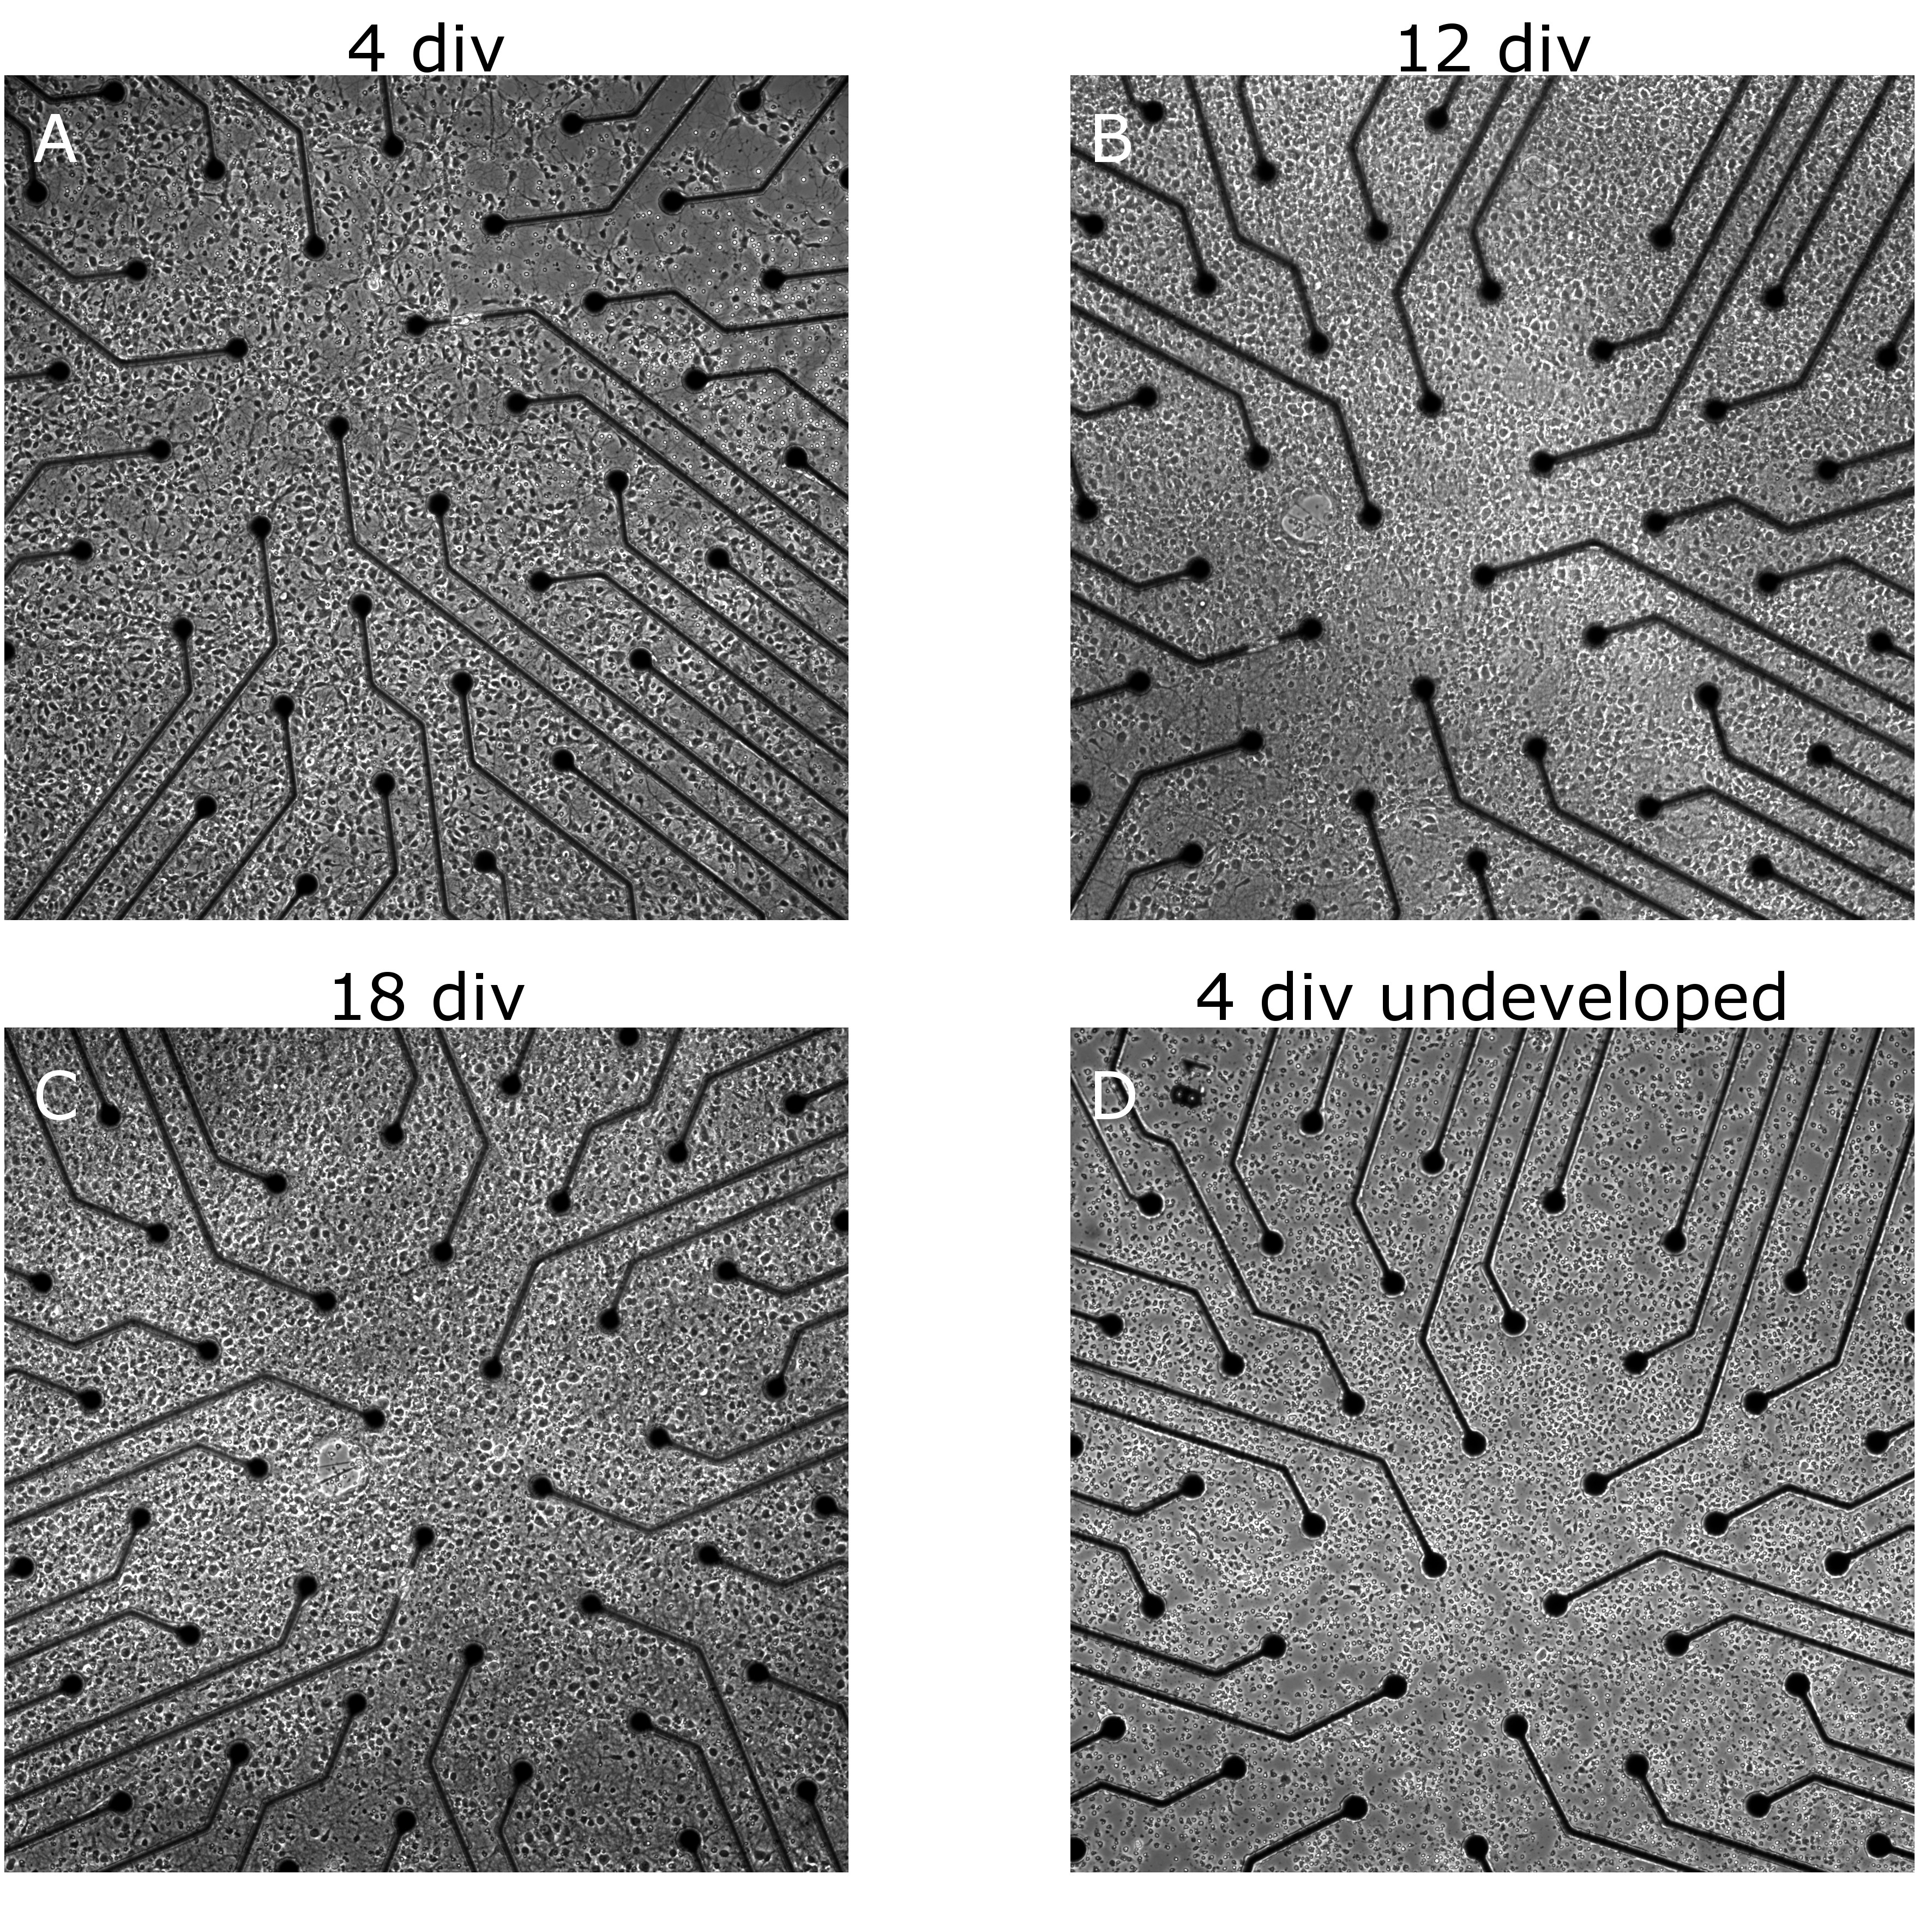
\includegraphics[width=15cm]{chapter3/figures/mouseImages/mouseImages.jpg}

            \caption[Representative images of a cortical mouse culture developing on a planar multi electrode array]{\textbf{Cortical mouse cultures develop to become a densely interconnected neural tissue.} (A) Cortical culture prepared from mice embryos, plated on micro-electrode arrays and imaged at 4 days in vitro. Arrowheads point to culture areas devoid of cell bodies where extending neurites may be observed. (B) Same location in the culture shown in panel A imaged at 16 days in vitro. At this point, individual neurites could not be observed even in areas no harboured by cell bodies (arrowheads), possibly due to the density of the neuritic mass or to engulfment by ECM. (C) The culture shown in panels A-B imaged in lower magnification for reference. (D) Example of a seeded culture that did not show proper development. In such cases, the seeded cells remained mostly circular indicating a lack of surface adhesion and little or no neurites were observed between the cell bodies (compare with A). The electrodes were \(30 \mu m\) wide and spaced \(200 \mu m\) apart.}
            \label{fig:activity:mouseImages}
        \end{figure}




    We monitored the spiking activity of the mouse cultures for 3 weeks in \textit{in vitro}. The analysis performed throughout this thesis is restricted solely to spiking activity and lower frequencies associated with local field potentials were filtered out of the data as this was considered sufficient for a first stage of characterization. Spike detection was preformed through a combination of match filtering and simple threshold crossing. A second pre-analysis step detected and removed erroneous spike waveforms induced by electromagnetic noise and which generated synchronized spiking artefacts across several channels (see section \ref{sec:methods:MEARecording} for full description of the pre-analysis). No spike sorting was attempted as this has been shown to be ineffective in culture \cite{herzog2011optical}.

        \begin{figure}[!htb]
            \centering
            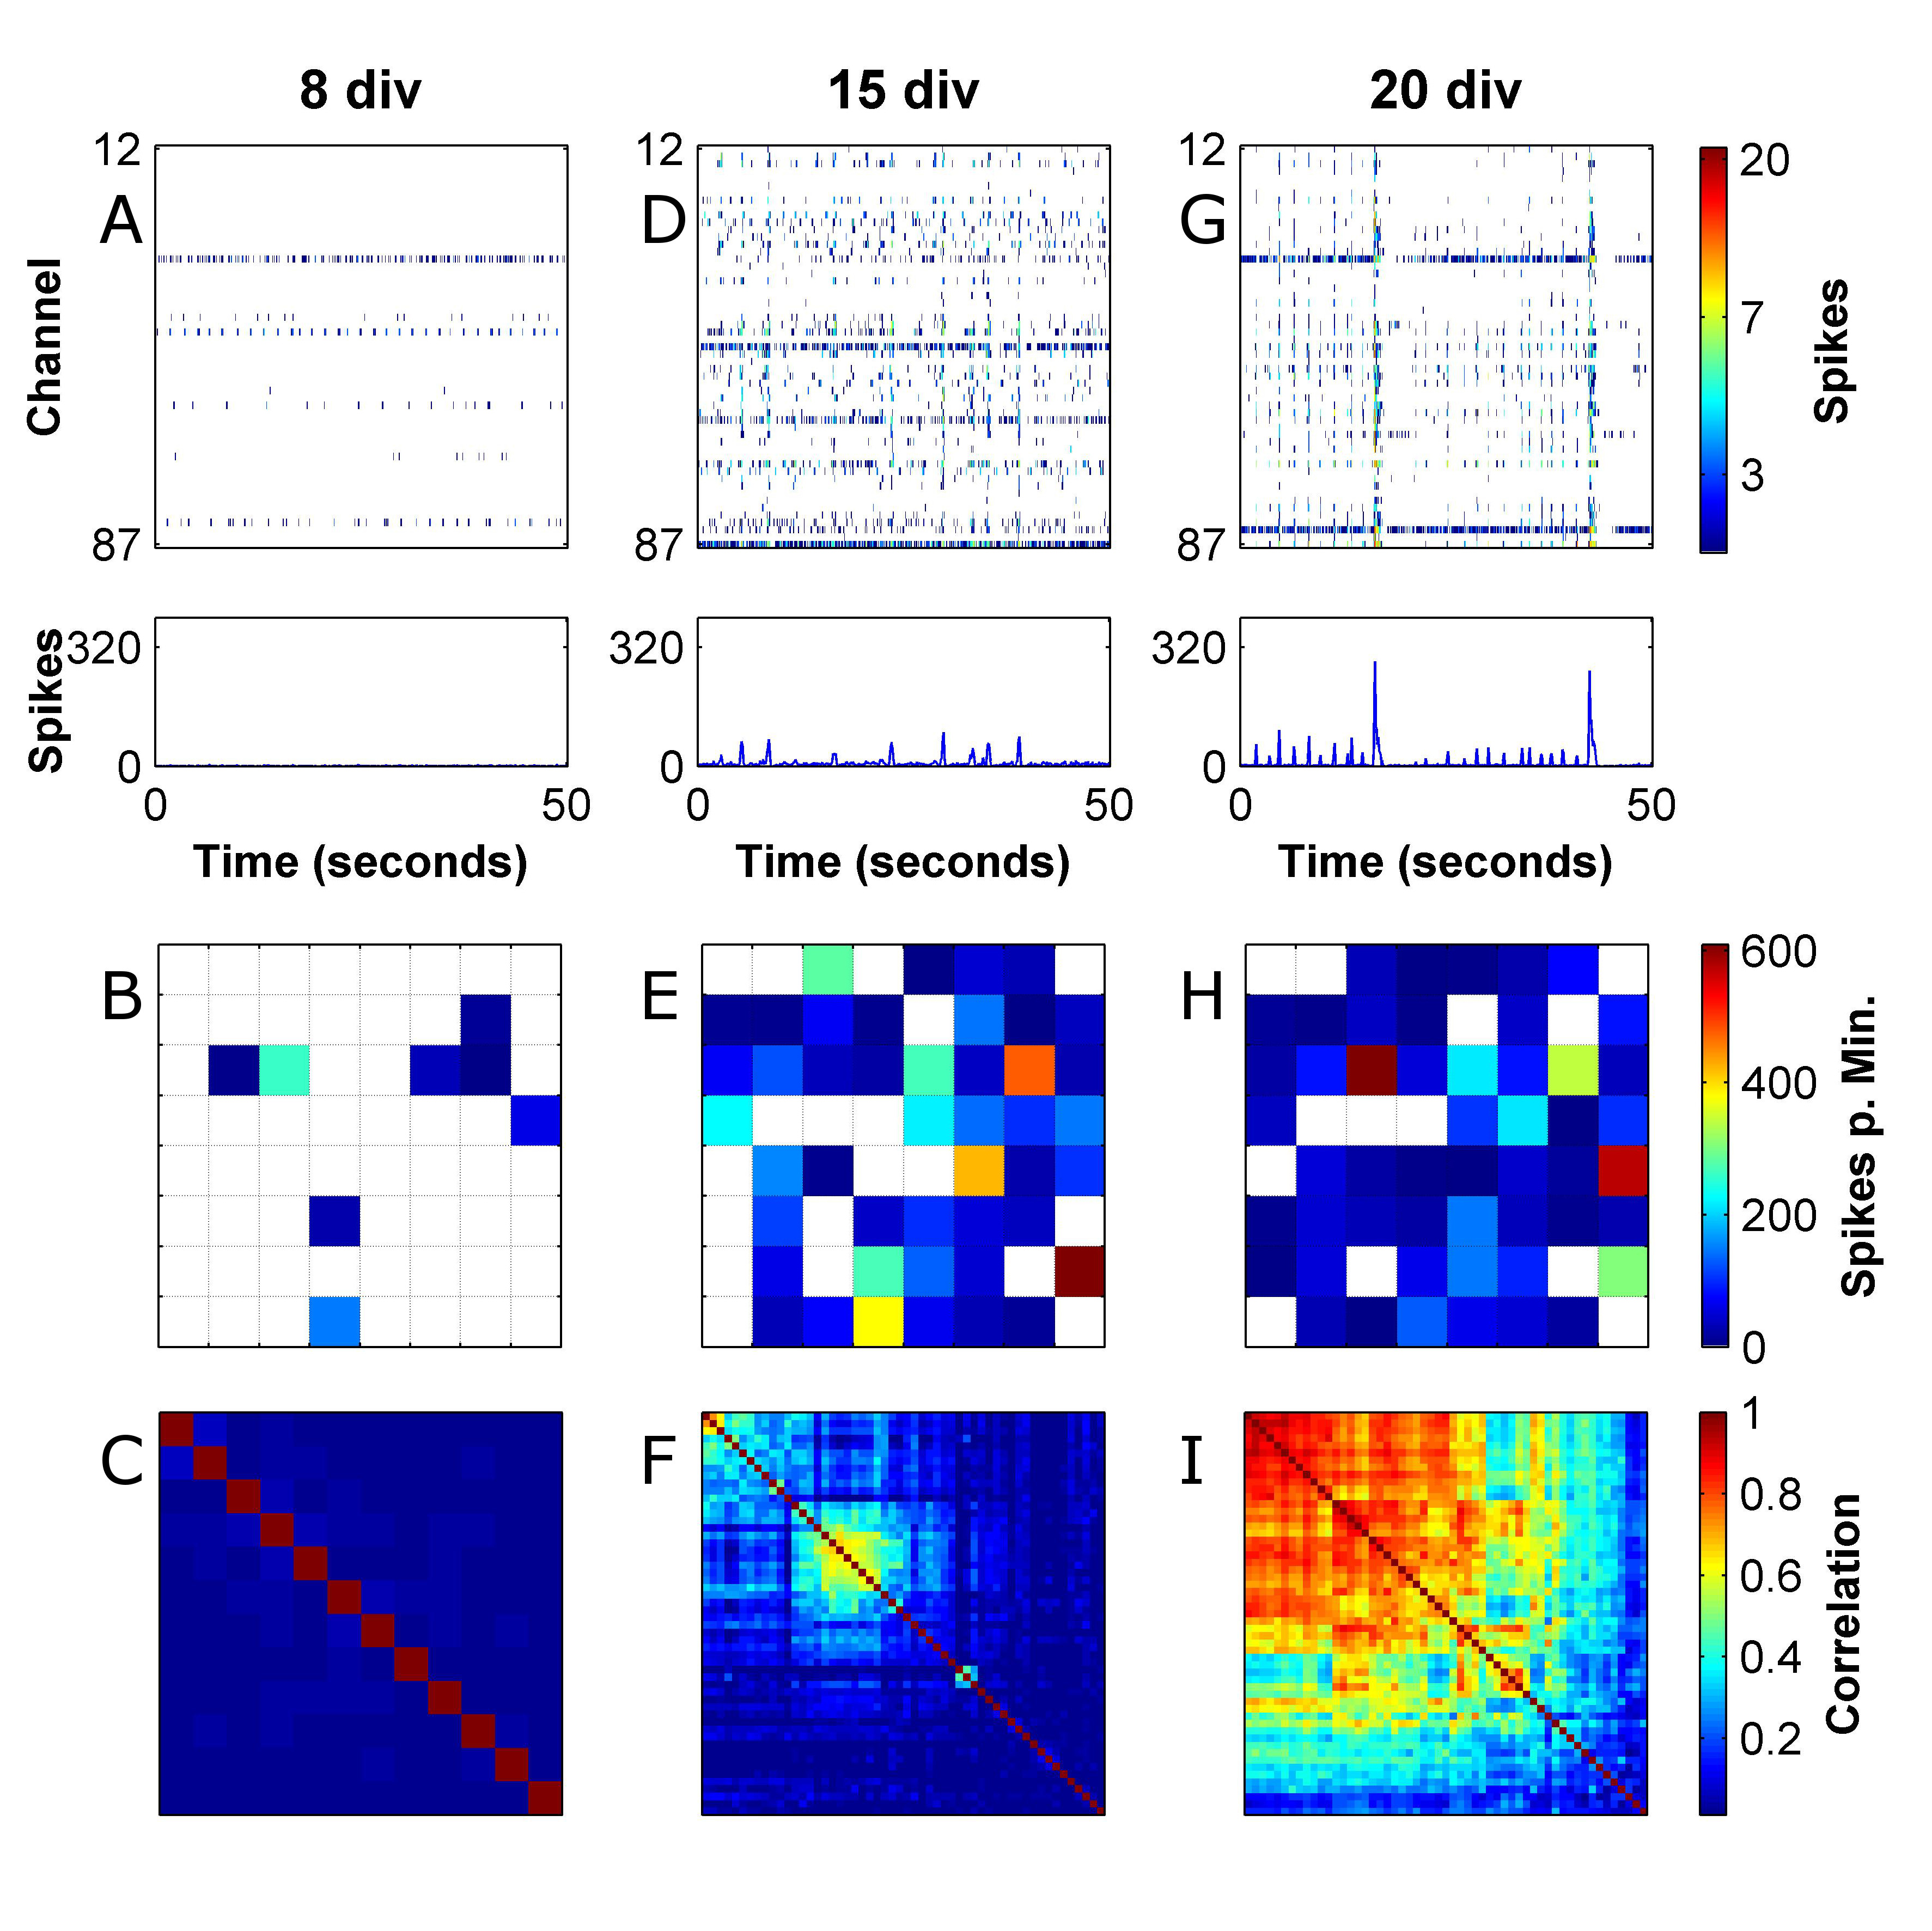
\includegraphics[width=15cm]{chapter3/figures/devExample/devActivity.jpg}

            \caption[Development of synchrony in the spontaneous activity of a representative mouse culture]{\textbf{Spontaneous activity in mouse culture develops from tonic firing into synchronized bursting events.} (A,D,G) Raster plot of spontaneous activity in mouse culture in 3 developmental time points exhibiting the change in the activity structure. Over development, network spiking activity gradually spread to most of the channels and became organized in network bursts. Raster plots are presented in \(100 ms\) bins. Bottom panels show sum of all channels. (B,E,H) Activity maps showing the spatial organization of activity on the MEA in the same time points. (C,F,I) Dendrogram- sorted correlation matrices showing groupings of channels into correlated blocks. Development of synchronization was manifested as blocks of correlated channel in the correlation matrix. Initially, several  correlated blocks were observed encompassing a subset of the channels, but these finally united to form a single correlated unit.}
            \label{fig:activity:devExample}
        \end{figure}



    Virtually no spikes were observed until approximately 5 days \textit{in vitro}, at which point tonic firing started to emerge in some of the channels. Beyond this point, the proportion of active channels and measured activity increased until reaching a plateau at about 13 days \textit{in vitro} (figure \ref{fig:activity:actMeasures}). The development of synchronization in the cultures is exemplified in Figure \ref{fig:activity:devExample} which shows raster plots at several developmental stages along with the associated mean firing rate maps and dendrogram-ordered cross channel correlation matrices. At 8 days \textit{in vitro} only a small proportion of the channels was tonically active and showed regular spiking (figure \ref{fig:activity:devExample} A). At this point there was very little correlation across the channels suggesting that the measured spike trains are not driven by synaptic integration but rather controlled through intrinsic neuronal excitability. At 15 days \textit{in vitro} most of the MEA channels exhibited spiking activity (figure \ref{fig:activity:devExample} D). At this point some correlated spiking events (network bursts) began to emerge although most of the activity was still regular and uncorrelated. These network bursts were not easily discernible in the multi channel raster plot but were evident as large peaks in the summated network activity and as increased correlations between a subset of the channels. To determine whether correlations of this magnitude could arise through chance, we generated surrogate independent spike rasters where the spikes trains were drawn from an independent Poisson processes with rate parameters as in the original channels (see section \ref{sec:methods:corrMaps}). In the surrogate data based on the recordings shown in figure \ref{fig:activity:devExample}, the maximal observed correlations between two different channels were 0.05, 0.05 and 0.07 for 8, 15 and 20 days in \textit{in vitro}, respectively. In the original data the maximal correlation values were 0.06, 0.7, 0.9, respectively. The significantly higher values observed in the original data for 15 and 20 days \textit{in vitro} and therefore indicate a genuine coupling between the measured neurons. Towards the end of the 3\textsuperscript{rd} week (here 20 days \textit{in vitro}) most of the spikes in the cultures were restricted to the network bursts (figures \ref{fig:activity:devExample} G and \ref{fig:activity:burstMeasures} E).

    During the early phases of synchronicity (beginning of 3\textsuperscript{rd} week, here 15 days \textit{in vitro}) it was common to observe more than one synchronized cluster of channels in the dendrogram-sorted correlation matrices (figure \ref{fig:activity:devExample} F). Nevertheless, correlations between these clusters continued to develop to the point where the entire culture became a single synchronized unit (end of 3\textsuperscript{rd} week, figure \ref{fig:activity:devExample} I). Previous work showed that applying synaptic blockers at non saturating quantities to fully developed neuronal cultures reveals an underlying modular connectivity pattern through breaking the weaker links between modules while still preserving denser intra-module connections \cite{breskin2006percolation}. Our results are compatible with this notion of underlying modularity and show that the modules are formed at the earlier stages of synaptic maturation.


        \subsection{Statistics of activity and synchronicity measures}
        \label{sec:activity:activityStats}

        Figure \ref{fig:activity:actMeasures} shows activity related statistics over our experimental data set comprising 5 mouse cultures. Long term electrophysiological studies of this type have been facilitated by the introduction of the MEA technology which easily allows sampling of multiple cells in parallel and repeatedly over long stretches of time. Intracellular microelectrode electrophysiology, in contrast, is usually restricted to a few cells at a time and cultures have to be discarded after a single experimental session as it is harder to maintain the cells healthy and sterile.

       \begin{figure}[!htb]
            \centering
            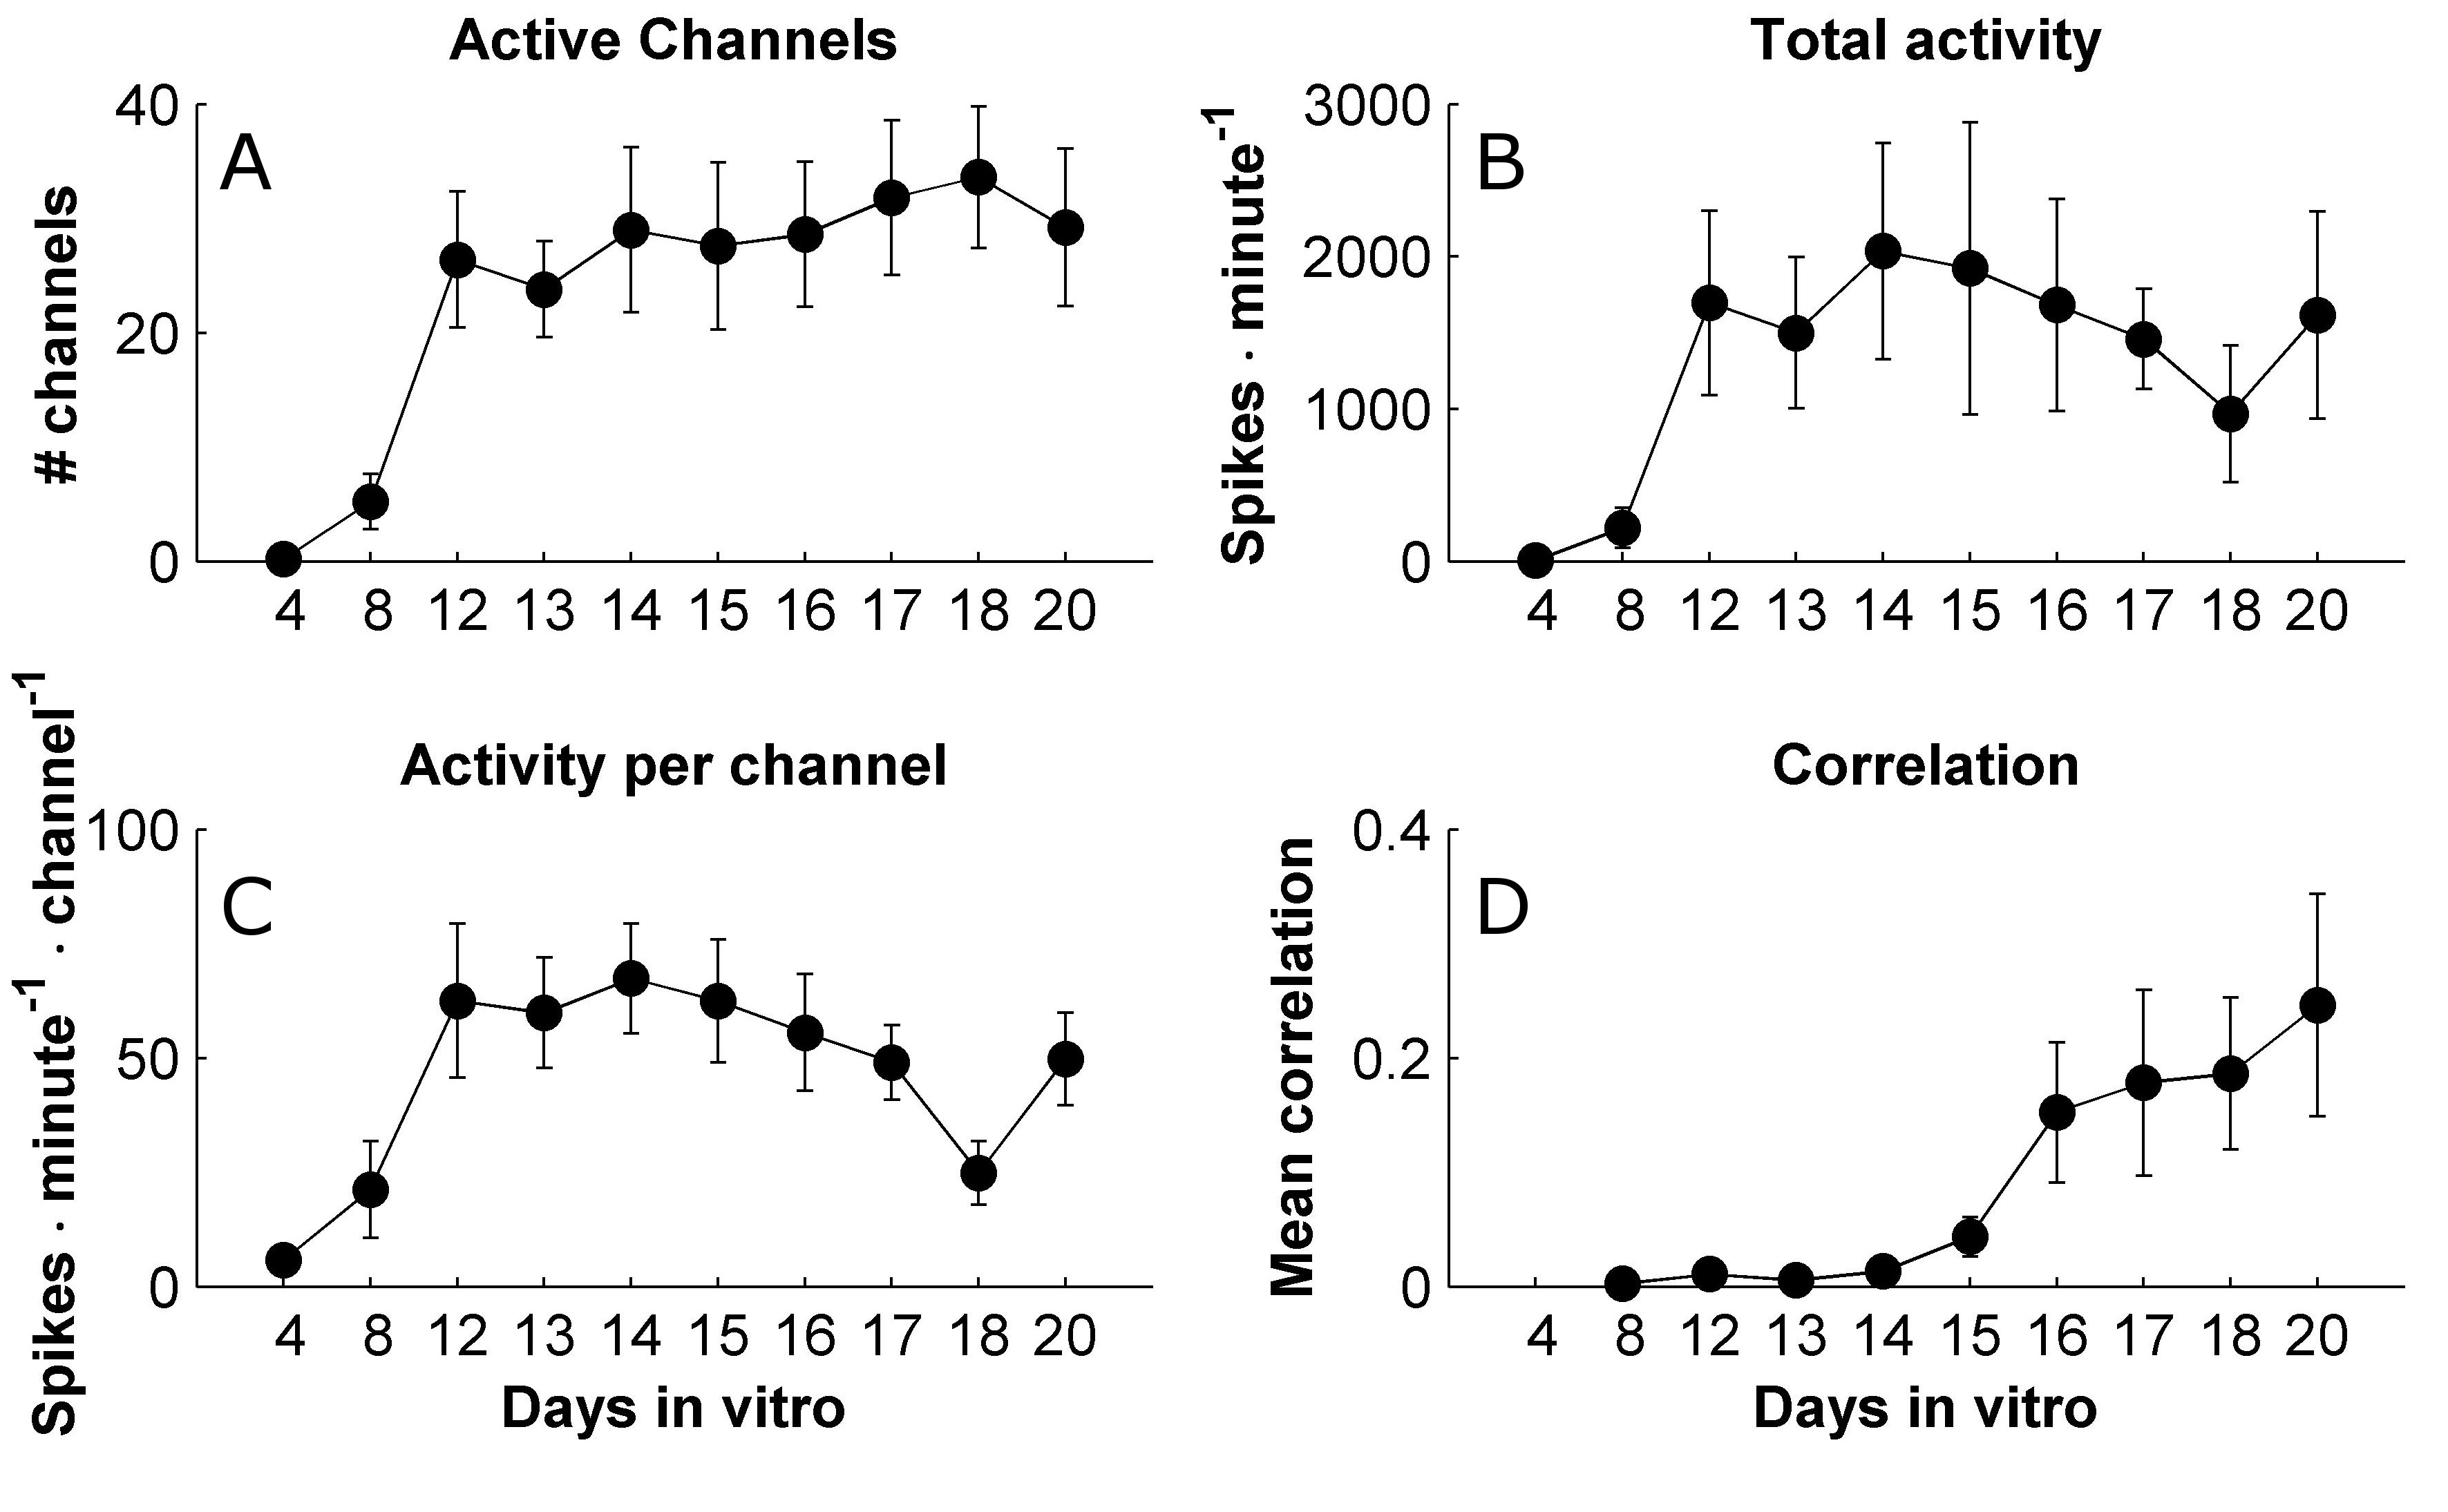
\includegraphics[width=15cm]{chapter3/figures/actMeasures/actMeasures.jpg}

            \caption[Averaged statistics of development of activity measures in mouse cultures]{\textbf{Development of synchronicity in mouse cultures lags after activity.} (A) Development of the number of active channels as a function of culture age. (B) Development of the total number of spikes recorded on all MEA electrodes. (C) Development of the mean neuron firing rate computed as average of firing rate over active channels. (D) Development of mean correlation over time. Mean correlation for a recording is the average of the correlation matrix taken excluding the diagonal. The data are shown as mean and SEM based on n=5 cultures.}
            \label{fig:activity:actMeasures}
        \end{figure}

        The cultures did not become fully active until approximately 2 weeks in culture suggesting that this period of time is required for the seeded progenitor cells to become mature excitable neurons (figure \ref{fig:activity:actMeasures} A-C). This time frame for activity onset is consistent with rat literature \cite{van2004long,wagenaar2006extremely,chiappalone2006dissociated} and is generally accepted with regard to culture electrophysiology where recording are typically performed at least 10 days into development.  After the initial increase, the firing rates (figure \ref{fig:activity:actMeasures} C) stabilize at around \(1 Hz\) and do not exhibit a time dependent trend (1-way ANOVA, p=0.3). The average firing rate per channel is compatible with studies from rat cultures which reported values in the range of \(0.4-1.5 Hz\) \cite{chiappalone2006dissociated,van2004long,corner2002physiological,penn2016network} but the lack of trend is different as rat cultures are reported to show a marked increase in individual firing rates until 21 days and a decline afterwards \cite{chiappalone2006dissociated,bikbaev2015brain}.

        Figure \ref{fig:activity:actMeasures} D shows the development of correlations in our cultures. The correlation value for a given recording is the mean of the correlation matrix (e.g., figure \ref{fig:activity:devExample} C,F and I) without the diagonal. Evidently, despite the stabilization of the mean unit firing rates at day 13 \textit{in vitro}, significant correlations started to arise only from about 17 days \textit{in vitro}. This suggests that the excitability in the cultures is initially controlled by intrinsic homeostatic mechanisms which are later replaced by synaptic drive. Remarkably, the apparent increase in synaptic efficacy is not accompanied by an increase in spiking activity suggesting that the unit mean firing rate of \(1 Hz\) is a controlled quantity which the neurons maintain in the face of a changing network environment around them. Indeed, it has been shown that cultured neurons are capable of rapidly modifying their intrinsic excitability in response to pre-synaptic blockers \cite{penn2016network}.


        To further characterize the spontaneous activity in the cultures we employed a burst detection algorithm as detailed in section \ref{sec:methods:burstDetection} and extracted parameters of burst related measures, shown in figure \ref{fig:activity:burstMeasures}. Not surprisingly, the development of bursting activity followed the same pattern as mean correlation and trailed the development of activity by a few days (figure \ref{fig:activity:burstMeasures} A,D compared to figure \ref{fig:activity:actMeasures} A-C). This separation between measures of individual activity and of of synchronicity underlines the utility of the MEA system in recognizing and disentangling biological processes that are linked. Previous rat cultures studies report that regular bursting is apparent already towards the end of the 2\textsuperscript{nd} week \textit{in vitro} \cite{van2004long,wagenaar2006extremely,chiappalone2006dissociated,bikbaev2015brain} whereas in our mouse data this was rare. In these reports the evolution of bursts appeared to go hand in hand with the evolution of activity, both of which peaked at 21 days \textit{in vitro} and declined afterwards. As bursting behaviour in our data was a few days delayed and started in the middle of the 3\textsuperscript{rd} week \textit{in vitro} it is plausible that a similar trend (but delayed) would be observed had we recorded further into the 4\textsuperscript{th} week.

      \begin{figure}[!htb]
            \centering
            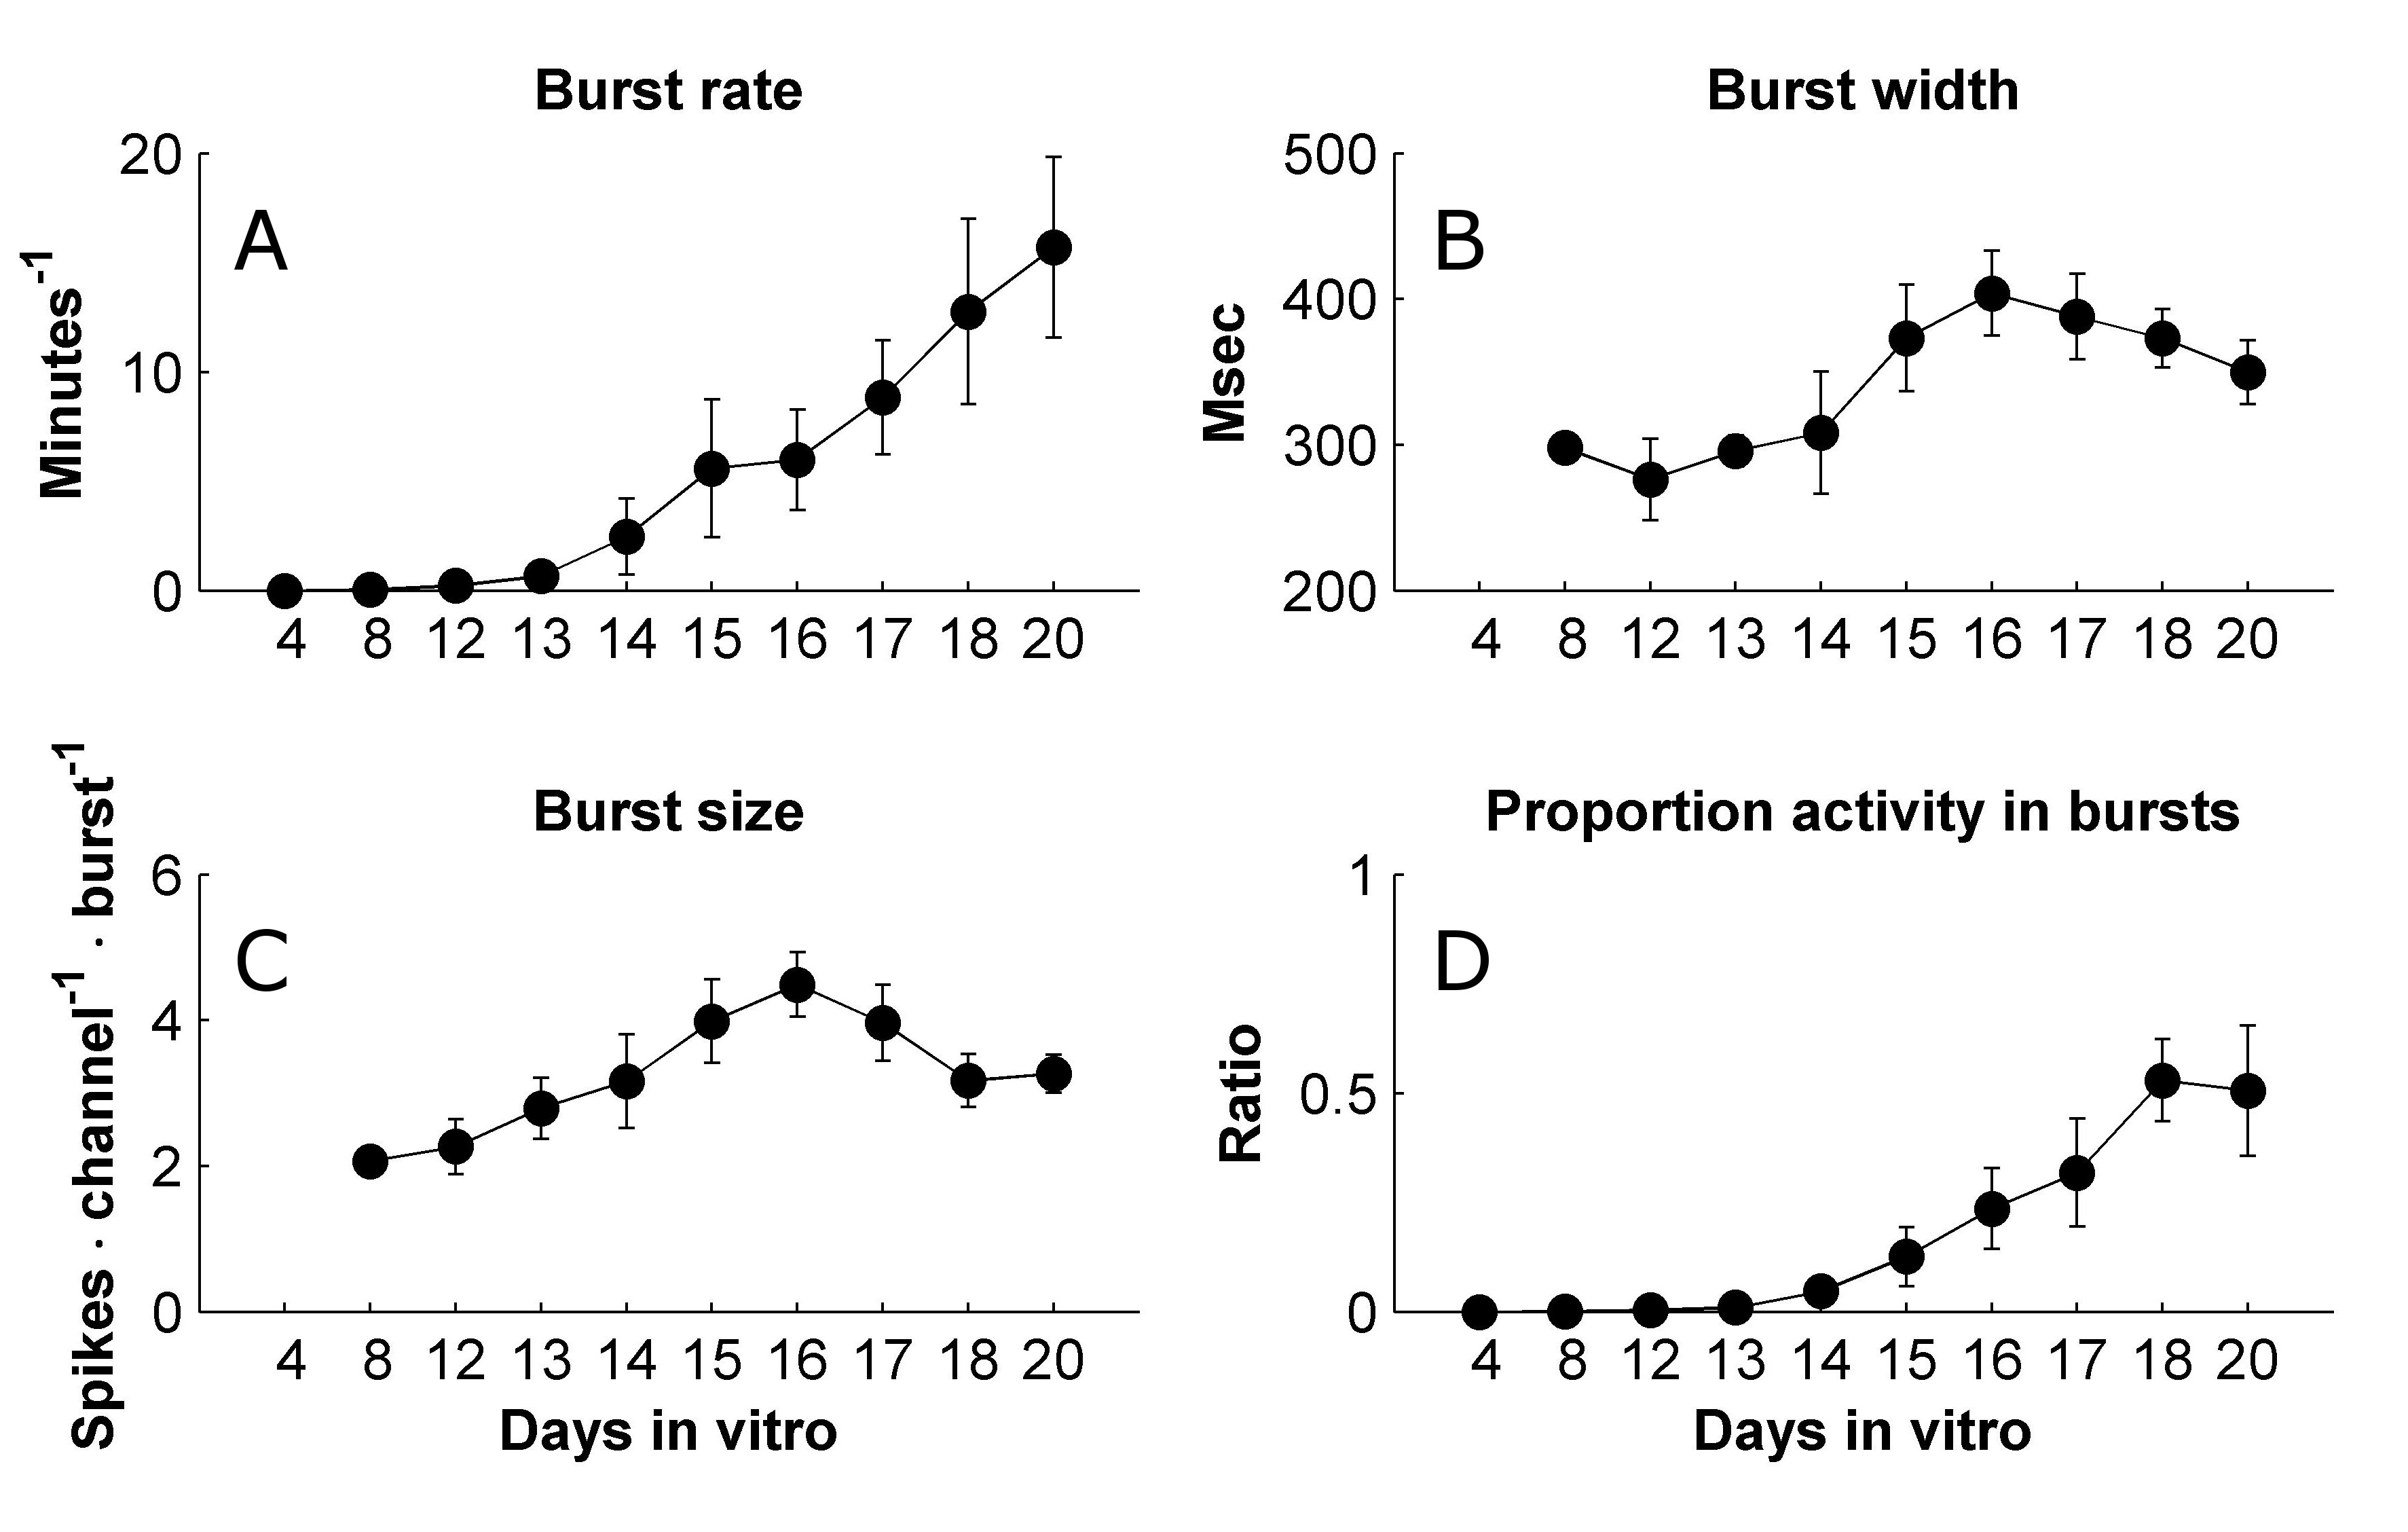
\includegraphics[width=15cm]{chapter3/figures/burstMeasures/burstMeasures.jpg}

            \caption[Averaged statistics of development of bursting measures in mouse cultures]{\textbf{Development of bursting measures in mouse cultures lags behind activity}. (A) Development of burst rate as a function of culture age. (B) Development of burst width. (C) Development of burst size. (D) Development of the ratio between the number of spikes observed within bursting events and the total recorded spikes. Data is shown as mean and SEM based on n=5 cultures.}
            \label{fig:activity:burstMeasures}
        \end{figure}

        It should be noted that the peak burst rate value observed (15 minute\textsuperscript{-1}) was much higher than the one reported for rat cultures at the same age of development (5 minute\textsuperscript{-1}) \cite{chiappalone2006dissociated}. However, we do not believe that this strong discrepancy lies in the difference between the preparations. Rather, our burst detection algorithm (section \ref{sec:methods:burstDetection}) uses an innovative approach for identifying synchronized events. Our method computes surrogate spike rasters with identical firing rates as the original data but without correlations to define the burst detection threshold. The thresholds defined in this way are likely to be tighter than for previous approaches where the thresholds were manually selected based on personal preference of how well they fit the data \cite{wagenaar2006extremely,chiappalone2005burst}. Since our thresholds are based on an objective criteria we argue that the observed burst rate indeed reflects synchronized events and that the rate of these is actually greater than previously reported. In section \ref{sec:activity:mouseRatComp} we will show a direct comparison between mouse and rat data which further supports the above argument.

        Further evidence for delayed synaptic maturation is provided by the burst width and burst size measures. Previous work has established that bursts in naive rat cultures exhibit wide temporal profiles with long tails of spike discharges that could last up to several seconds \cite{chiappalone2006dissociated,van2004longterm}. Over the 3\textsuperscript{rd}-4\textsuperscript{th} weeks the burst profiles become narrow and exhibit increasingly faster termination until saturating in the end of the 4\textsuperscript{th} week. This change is attributed to the development of the GABAergic neurotransmission which was shown to occur 1-2 weeks in delay as compared to the glutamatergic system \cite{ramakers1994activity,swanwick2006development}. Hence it has been postulated that feedback loops operating through inhibitory interneurons become functional only in the aforementioned time period  \cite{van2004long} (3\textsuperscript{rd}-4\textsuperscript{th}, also see an \textit{in vivo} correlate in \cite{hensch2005critical}). In the rat data the bursts show maximal width when they first appear (10-14 days \textit{in vitro}). In our data, a similar trend is observed with peaks appearing in the burst size and burst width measures at 17 days \textit{in vitro}, which is approximately the point when bursting activity became appreciable (time effect was found significant through 1-way ANOVA for both burst size and burst width measures with p=0.035 and 0.028, respectively).

        Another known phenomena where the differences between mouse and rat cultures seem to be manifested are `superbursts'. These refer to periods of elevated activity with epileptiform-like discharges seen in rat cultures in the second and third weeks \textit{in vitro} \cite{wagenaar2006extremely}. These unrestrained firing patterns disappear later on in development, presumably upon the delayed maturation of the inhibitory system mentioned above (see also section \ref{sec:introduction:MEANetwork}). Such superbursts have not been observed in any of the mouse cultures followed here for 3 weeks \textit{in vitro} but were very common in the rat cultures used throughout the following chapters. This observation provides further support to the notion that excitatory synaptic transmission in mouse cultures develops more slowly and might be more effectively balanced by the concurrently developing inhibition.

        Taken together, the results from the spontaneous activity study demonstrate that, on one hand, the development of neurotransmission and synaptic connections in our mouse cultures appears to be delayed between 3 days to one week compared to reported rat cultures. On the other hand, irrespective of the delay, the cultures exhibit all the activity features expected from literature, such as, homeostatic control of excitability, underlying modularity and development of synchronicity and bursting activity which evolve in accordance with the development of the synaptic networks.


    \section{Evoked activity}
    \label{sec:activity:evoked}
    An important feature of the MEA technology is the ability to induce generation of action potentials through injection of a current waveform into the extracellular electrodes. This is an important functionality as it allows providing input to the network and to influence the culture activity. Past work has provided effective stimulation protocols and showed that short current pulses of several hundred \(\mu s\) can induce individual action potentials as well as a network response \cite{marom2002development,wagenaar2004effective}. This methodology was used to study response properties of single isolated neurons over long periods of time \cite{gal2013entrainment} and how several stimulation pulses interact with each other as a function of temporal proximity \cite{eytan2003selective,weihberger2013quantitative,baljon2009interaction}. This approach was also used to model sensory input by providing more complex spatio-temporal stimulation pattern and examining the extent to which the information present in the input signal can be decoded from the culture activity \cite{marom2009precarious,cozzi2006encoding}. Interestingly, it was shown that high frequency stimulation can break down the synchronized bursting structure of the culture activity, presumably in analogy to brain structures which exhibit higher frequency content and lower synchrony when subjected to a high volume of input during active sensory processing \cite{wagenaar2005controlling}.

        \begin{figure}[!htb]
            \centering
            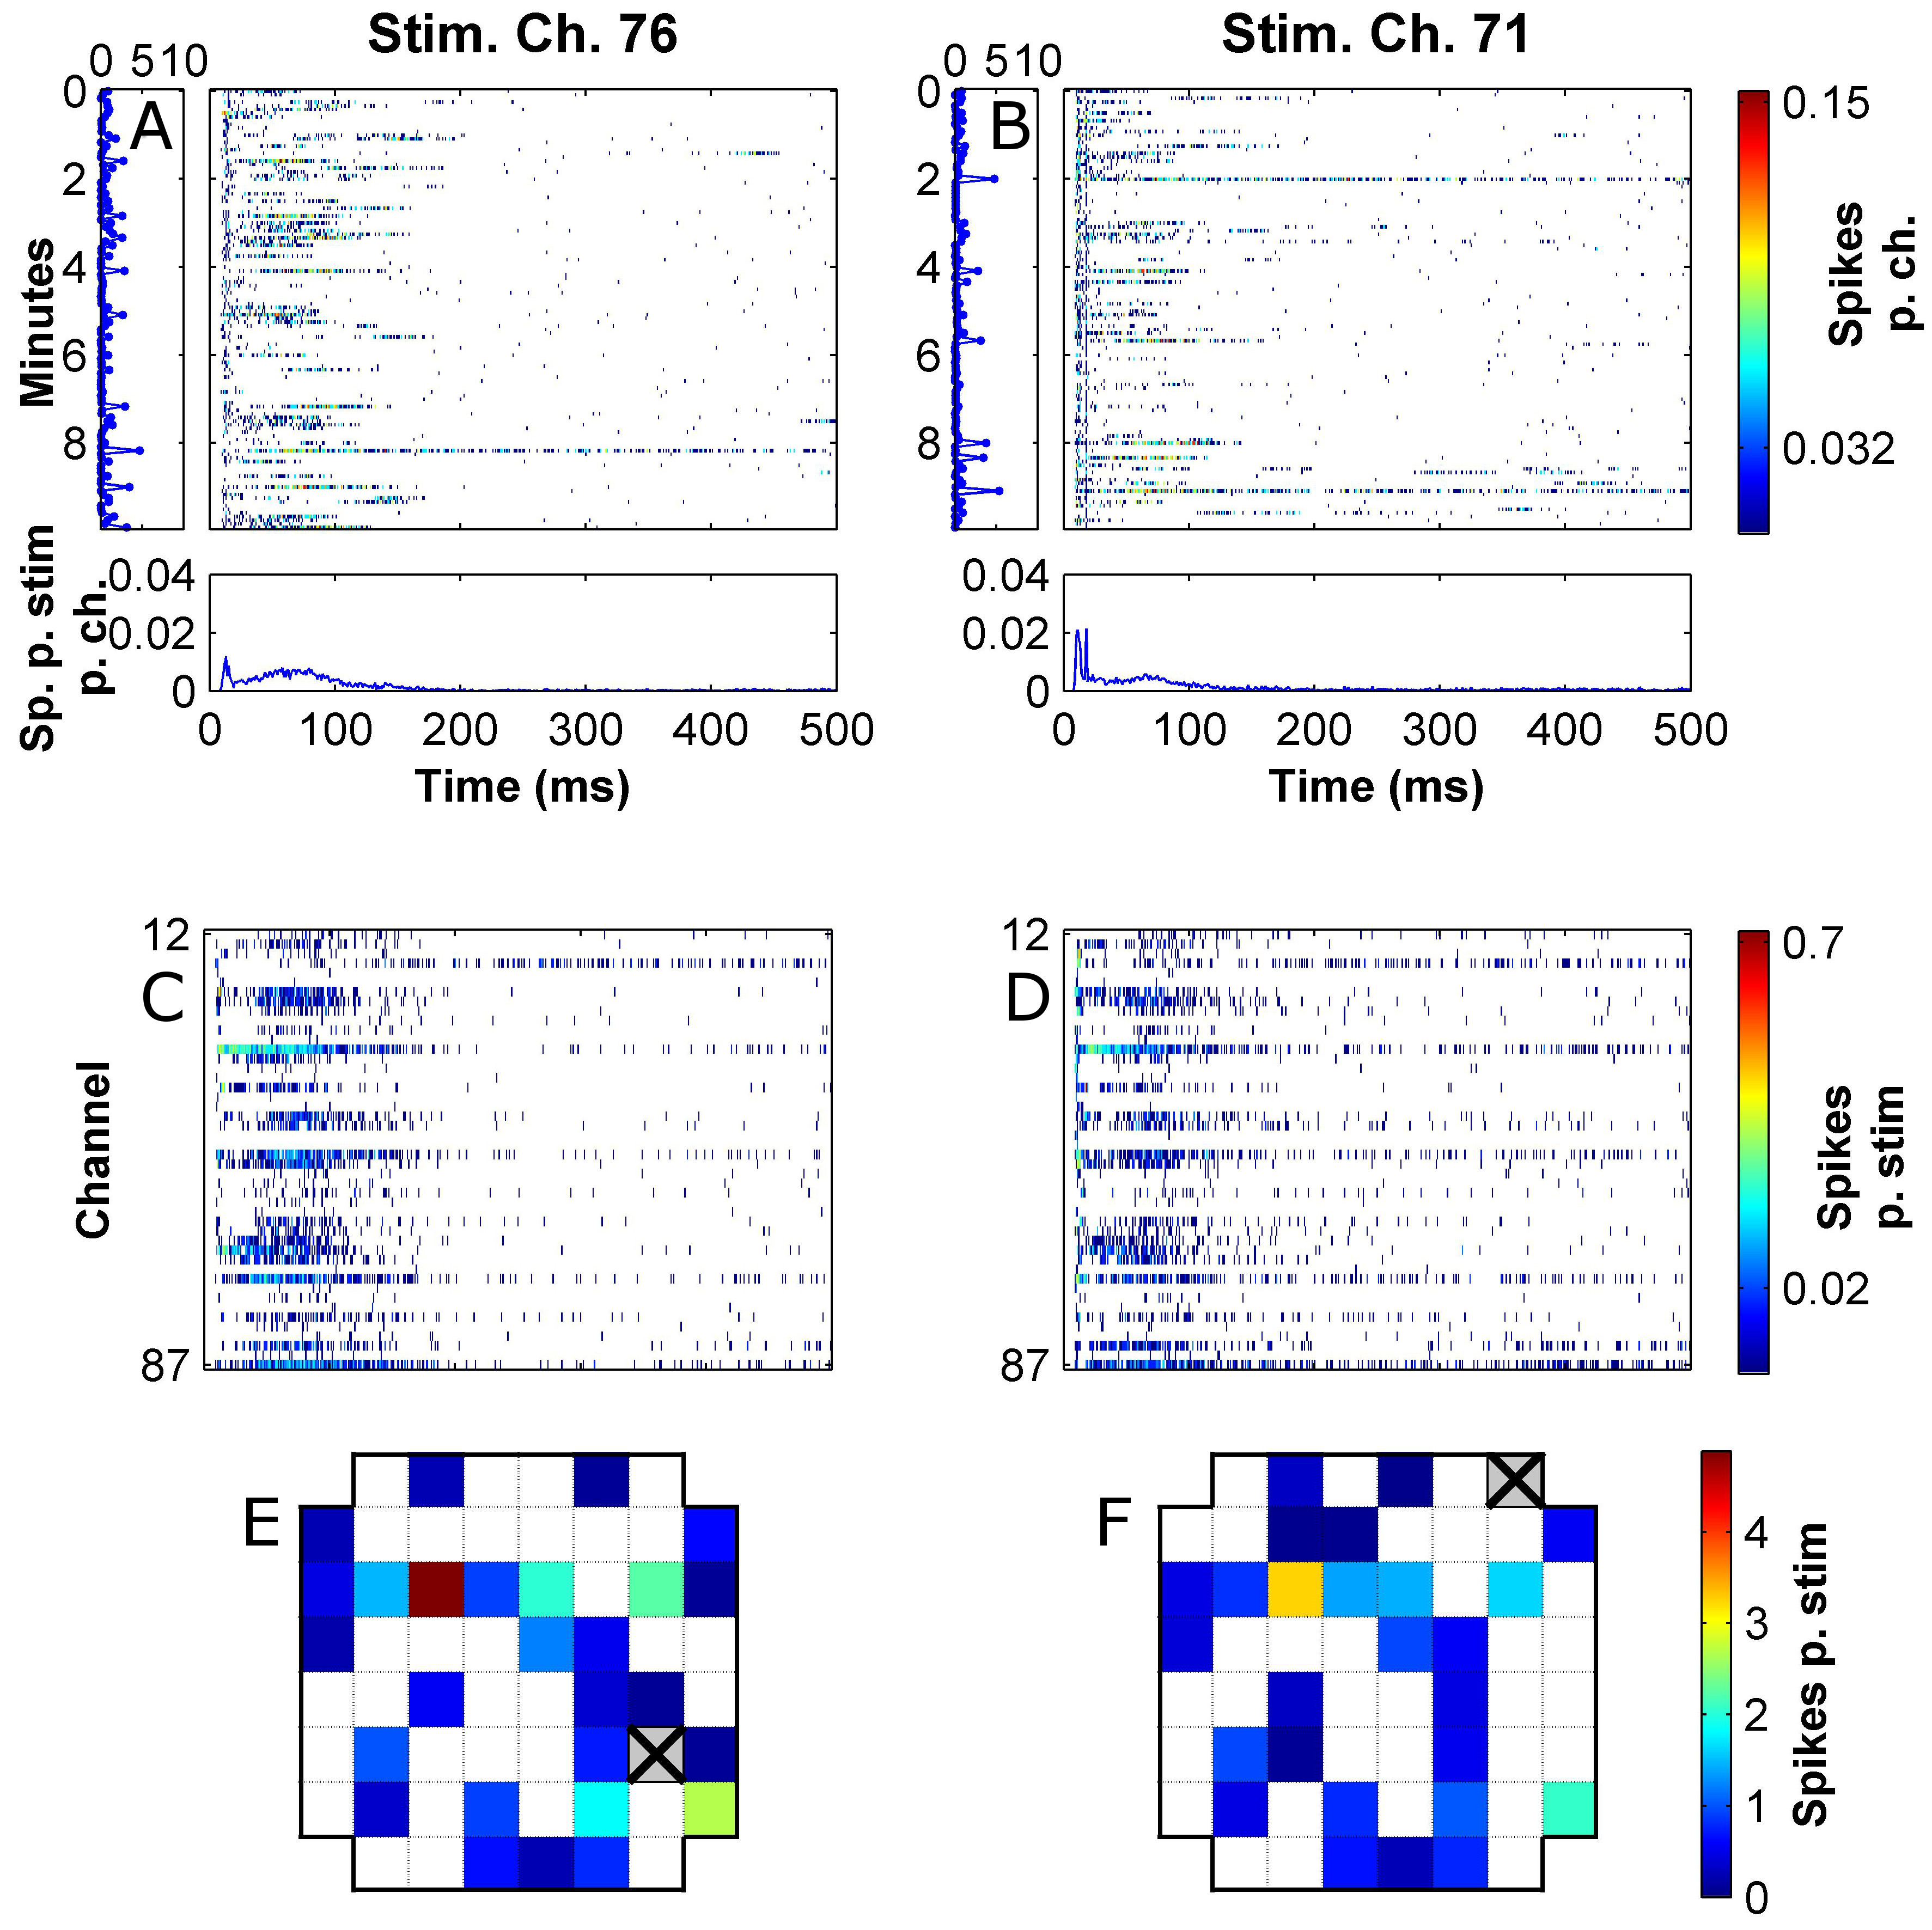
\includegraphics[width=14cm]{chapter3/figures/stimExample/stimExample.jpg}

            \caption[Example of responses to test stimuli applied at 2 different electrodes]{\textbf{Stimulation pulses at different electrodes vary in direct responses but produce a similar reverberative responses.} Test stimuli were applied every 5 seconds. (A-B) Main panel: Each line is a response raster for one test stimulus averaged over all channels. Left panel shows the sums of the responses shown in the main panel over the post stimulus observation time window (i.e., number of spikes per channel observed in 500 ms period post stimulation). Bottom panel shows the average of the response rasters over all stimuli. This is the PSTH. (C-D) Spatially resolved PSTHs, i.e., each line is a channel PSTH. The spatial profiles of the responses to the different stimulation sites are visually similar. (E-F) Stimulation response maps showing the sums of the PSTHs in (C-D) in the actual spatial locations. These response maps only show channels with a stimulation response that is significantly higher than background spontaneous activity for that channel (see section \ref{sec:methods:stim} for selection procedure). Stimulating electrodes are marked by an X on a gray background. A,C,E and B,D,F show response data for two stimulation sessions applied to two different electrodes (indicated in E,F) run one after the other in succession on the same culture. All raster plots use \(1ms\) bins.}
            \label{fig:activity:stimExample}
        \end{figure}

    To demonstrate that our system is able to effectively interface with the culture and provide input, we present data from a stimulation session where 120 test pulses were applied every 5 seconds to a single electrode (see section \ref{sec:methods:stim} for technical details). Data for two distinct stimulation sites (electrodes) are shown. Figure \ref{fig:activity:stimExample} A-B shows raster plots of the stimulation responses (at the different sites) averaged over all channels in a \(500 ms\) window after the stimulation pulse, as well as a PSTH, which is essentially the average of all individual responses (post stimulus time histogram). The PSTH was typical to what is normally observed in these preparations: a bimodal curve with a sharp peak observed within the first \(25 ms\) after stimulation and a second, significantly wider and less defined peak which typically lasts about \(200 ms\) after stimulation. The first peak is considered to represent direct responses, i.e., spikes elicited directly as a result of the stimulation pulse without synaptic mediation. The second peak is thought to be a manifestation of a multi-synaptic reverberating activity in response to the first step of activation. Indeed, it is evident from the response rasters that the first stage of response is significantly more repeatable than the second one which was not always present. This is compatible with the above interpretation as direct responses are spikes generated due to a stimulation induced localized depolarization and depend only the specific biophysics and geometry of the neuron so they are expected to occur at a set delay and with low jitter. The reverberating response, on the other hand, is a complex phenomena which depends on the network state preceding the stimulus so it stands to reason that it would show large variability or even fail to propagate on occasion. Nevertheless, it should be noted that even the direct responses were far from operating at a 100\% success rate, a single neuron reproducibility issue that has been under much debate within the neuroscience community \cite{mainen1995reliability,gal2013entrainment}.

    Comparing between the responses to the two stimulation sites it is evident that they differed in direct responses with stimulations in channel 71 producing a second direct response peak which is also observable as a vertical line in the response rasters. The reverberating response did not show conspicuous differences in shape or latency although it seemed somewhat smaller. Another view on the differences between the two stimulation sites is given in figure \ref{fig:activity:stimExample} C-F which show spatially resolved response rasters (i.e., PSTHs of individiual channels) and response maps for all participating channels, averaged over the stimulations. The spatial response profile appears to be very similar when comparing the two different stimulation electrodes - each channel showed a similar strength and duration of activation. There are some differences in latency but these were relatively unpronounced, at least to the naked eye. Although we did not study this in depth, it was our impression that different stimulation electrodes differ in mainly whether they are were at all able to produce a reverberating response. However, once this response was elicited it seems to be stereotypical, i.e., each culture develops to take on an particular identity which is elicited whenever a synchronized burst occurs regardless of the site of induction or if it is spontaneous or evoked. It has been suggested that the lack of sensory input during culture development drives it into a degenerate state of over connectedness which might explain this rigidity. On the other hand, it should be noted that distinct yet overlapping responses to different stimulation sites have been reported \cite{wagenaar2006searching}. Additionally, decoding of spatial stimulation information from culture data has been successfully demonstrated \cite{kermany2010tradeoffs} so this system might nevertheless model genuine neural coding mechanisms from \textit{in vivo}.

    \section{Plasticity induction in the presence of dopamine}
    Mature neuronal cultures abide to the principles of spike timing dependent plasticity (STDP), demonstrated in a paired pulse paradigm \cite{bi1998synaptic}. This observation has raised the interesting possibility that neuronal cultures grown on multi electrode arrays could be used to study how plasticity operates at the network level. This sparked a substantial body of work to devise paradigms for induction and observation of plasticity using just extracellular network recordings and stimulations. Initial efforts have focused on brief tetanic stimulations inspired by the original experiments discovering LTP and which used this stimulation protocol \cite{bliss1973long}. Positive reports employing tetanus based induction have reported either a generalized potentiation in evoked responses which could be observed using simple measures such as summated response over all MEA electrodes \cite{chiappalone2008network,hamilton2015time,ruaro2005toward} or more subtle effect that did not involve global change but rather antagonistic changes to the different channels and required more sophisticated multi-variate analyses to observe \cite{jimbo1999simultaneous,le2015repeated,madhavan2007plasticity}. The latter type of plasticity was observed both in evoked responses as well as in spontaneous activity. Indeed that tetanus induces a global potentiation is not surprising given that the original LTP experiments involved potentiation in the LFP measurements which represent large populations of neurons. However, it is known that neuronal systems employ homeostatic mechanisms to keep the general excitation levels constant \cite{turrigiano1999homeostatic} so such extreme modifications to activity are likely to be unphysiological. In that sense it is interesting that more subtle forms of plasticity are observed in the multi dimensional aspect of the activity. However, it is unclear why similar protocols produce such differences in outcome in different studies and different labs. Later work has shown that low frequency stimulation protocols can also induce changes in spontaneous activity of the subtle type \cite{le2015repeated,vajda2008low}. This result is interesting as natural input during real-life behavioural learning is probably more similar to such low frequency signals than to tetanus. Obviously, behaviour in general and learning in particular are a closed loop process and this was modeled, to a certain extent, with feedback systems where the stimulation pattern was directly informed by the preceding neuronal activity \cite{bakkum2008spatio,shahaf2001learning}. These important works showed that the direction and extent of plasticity can be controlled to follow bespoke criteria and therefore established that they are indeed relevant for goal directed learning.

    As mentioned above, the quest to find plasticity in neuronal cultures grown in MEAs has produced successes but also contradictory, controversial and negative reports \cite{wagenaar2006searching,le2009slow}. Here we provide our own contribution to the discussion by applying one of the reported protocols
    to our mouse cultures and checking for plasticity. Additionally, as reviewed in section \ref{sec:introduction:neuromodulators}, neuromodulators have been shown to be strongly associated with neuronal plasticity and their presence or absence can strongly affect the direction of change (i.e., potentiation or depression) or even abolish it altogether (reviewed in section \ref{sec:introduction:neuromodulators}. Consequently it has been suggested that dopamine signalling is a missing ingredient required to facilitate consistent plastic processes in culture. Further support for this notion was provided by a culture study showing that dopamine modulates of the effective STDP window using intracellular recordings \cite{zhang2009gain}. Since neuromodulators have not been used in conjunction with plasticity and neuronal cultures on MEAs we decided to include a phase within our protocol where dopamine is introduced just for the induction period and washed away afterwards. The reason for washing the dopamine away was to avoid mistaking its direct modulation of the activity to be synaptic plasticity. Additionally, since neuromodulators signal the occurrence of a salient or rewarding events we intended this paradigm to model a situation where such rewarding event occurs during the tetanus.

    We elected to use a tetanus induction protocol based on \cite{chiappalone2008network}. The reasons for selecting this protocol are as follows: Firstly, some of the past plasticity work on MEAs did not include a control to verify that the observed changes are due to the stimulated activity and not an artefact. Although this may seem unscientific it is a consequence of the nature of the system where each sample takes a long time to produce, maintain and measure. As a result, achieving a high n-number for both experiment and control is in some cases impractical. Our protocol works around this by exploiting the fact that neuronal cultures on MEAs can be used continuously for many recordings without compromise so we ran all experimental and control sessions on the same culture consecutively. Secondly, more complicated protocols such as the ones that apply stimulation in feedback from the recorded activity would require a sophisticated drug application system which is not currently available. This protocol includes a tetanus epoch of just a few minutes which offers a convenient time frame for manual addition and washing away of the drug.

        \label{sec:activity:plasticityProtocol}
        \begin{figure}[!htb]
            \centering
            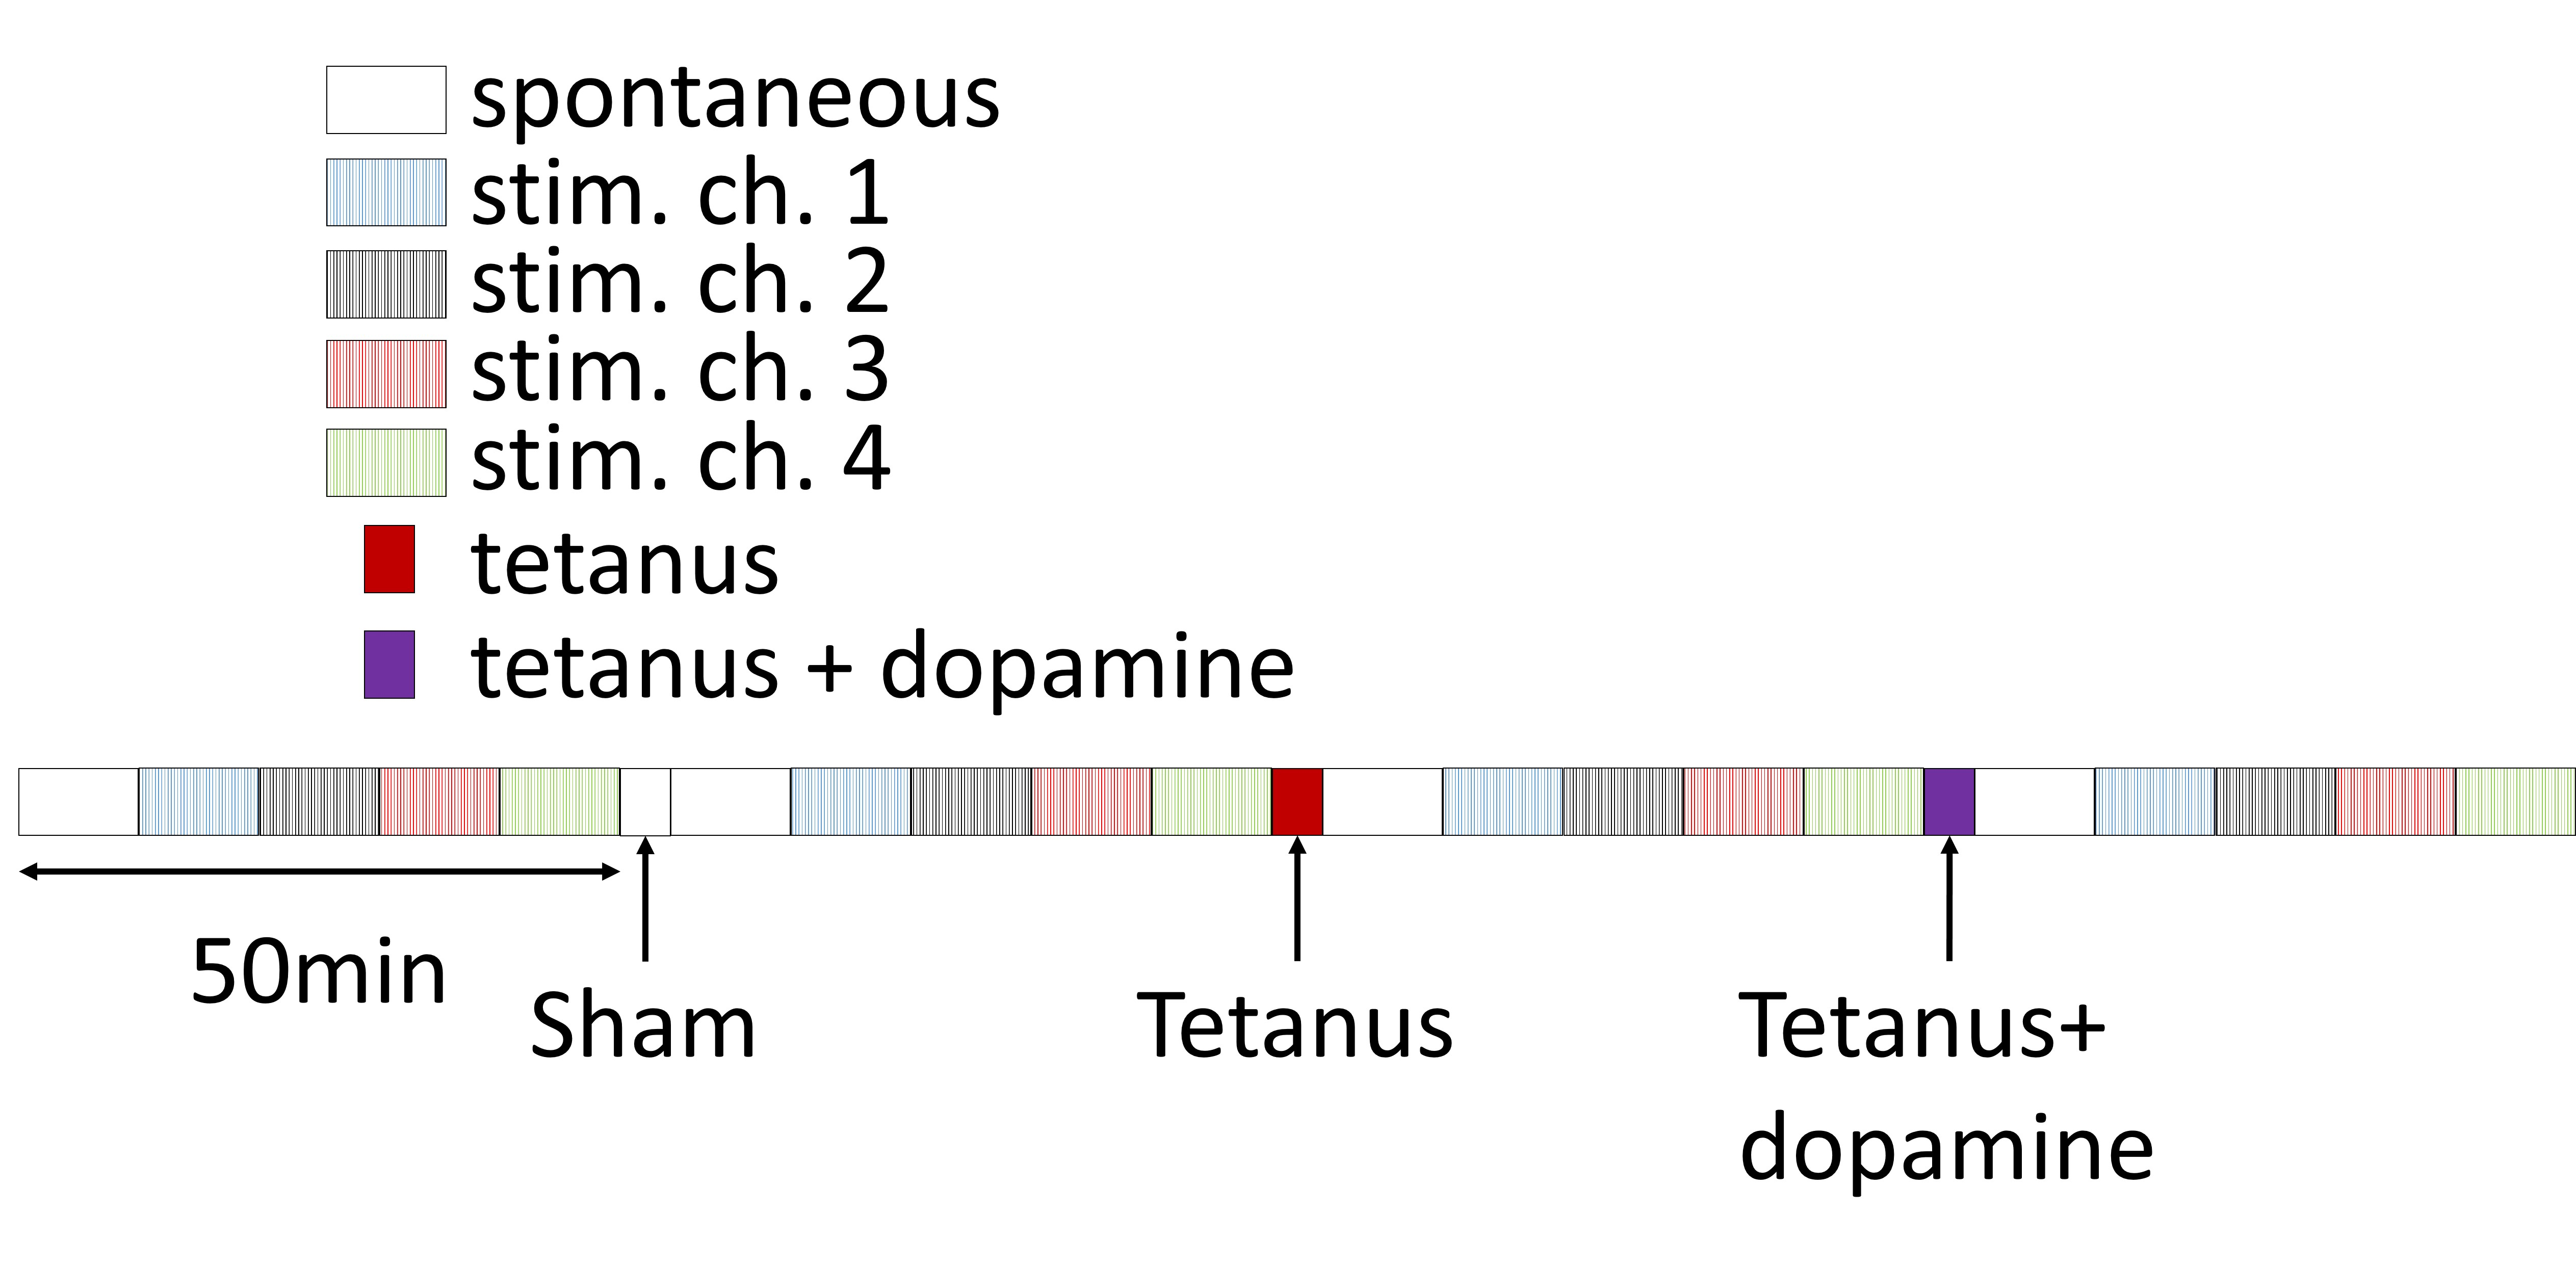
\includegraphics[width=15cm]{chapter3/figures/ExpOutline/expOutlineTet.jpg}

            \caption[Outline of the combined dopamine-and-tetanus-induced open bath plasticity experiments]{\textbf{Outline of the combined dopamine and tetanus open bath plasticity experiments.}}
            \label{fig:activity:expOutline}
        \end{figure}

    Figure \ref{fig:activity:expOutline} shows a schematic of the experiment. The protocol catered for examination of both spontaneous activity and evoked responses. Each measurement epoch comprised a period of 10 minute recording spontaneous activity, followed by 4 x 10 minute periods of recording under 0.2 Hz test stimuli applied at 4 different electrodes, respectively. The electrode identities and amplitudes of test stimuli were selected to produce obvious evoked responses based on a pre-experiment examination. The measurement epochs were separated by 3 induction epoch running an 'associative tetanus' as proposed by \cite{chiappalone2008network}. 'Associative tetanus' is a stimulation paradigm designed to induce an association between two stimulated populations. The primary channel produces a tetanus pulse train consisting 50 pulse sets at \(0.2 Hz\) each consisting of 50 pulses at \(20 Hz\). The secondary channel produces 50 single pulses at 0.2 Hz in phase with the tetanus pulse sets, i.e., each stimulation pulse in the secondary channel is timed to occur in the middle of a set in the primary channel. The primary and secondary channels were selected randomly out of the 4 stimulation channels used in the measurement epochs. The 3 induction epochs are as follows: (1) a sham (control) 'associative tetanus' executed by the signal generator with pulses of \(0 mV\) amplitude. (2) An actual 'associative tetanus' where the amplitudes for the primary and secondary channels are the same as those used in the test stimuli in the same channels during the measurement epochs. (3) An 'associative tetanus' as above where half of the culture media (\(0.5 ml\)) was first removed for later use and \(100 \mu M\) dopamine was added. After the termination of the tetanus the dopamine containing media was replaced with the portion earlier removed and the final examination epoch was carried through. It should be noted that removal of half of the media during the 3\textsuperscript{rd} induction epoch caused a slight but noticeable increase in the recording noise so the spike detection thresholds in the earlier measurement epochs were matched to the last one to avoid biasing of the results.

    \subsection{Examining changes in response to stimulation}
    Figure \ref{fig:activity:tetStimChange} shows example stimulation response data for the 4 measurement epochs in one of the tested cultures. Data is presented as explained in section \ref{sec:activity:evoked}. Baseline refers to the initial measurement epoch performed prior to any induction epoch. Control refers to the epoch taking place after the sham tetanus and the differences from the preceding epoch reflect spontaneous deviations in the culture activity. Tetanus and tetanus + dopamine are the epochs following the genuine induction phases. The differences between these experimental epochs and their immediate predecessors are compared to the difference between the control and baseline epochs so as to capture the effect of the induction. The baseline, control and tetanus epochs all show a similar PSTH profile and similar channel rasters. However, there are also some noticeable differences. For example, the latency of the reverberating response seems to increase approximately half way through the control epoch, a change that is carried over to the tetanus epoch. Additionally, the reverberating phase in the control PSTH is smaller than in the baseline and this is observed as reduced intensity in some of the channel rasters. These spontaneously occurring changes (i.e., not associated with the tetanus induction) highlight the importance of employing such control epochs to assess how activity features change spontaneously.

        \begin{figure}[!htb]
            \centering
            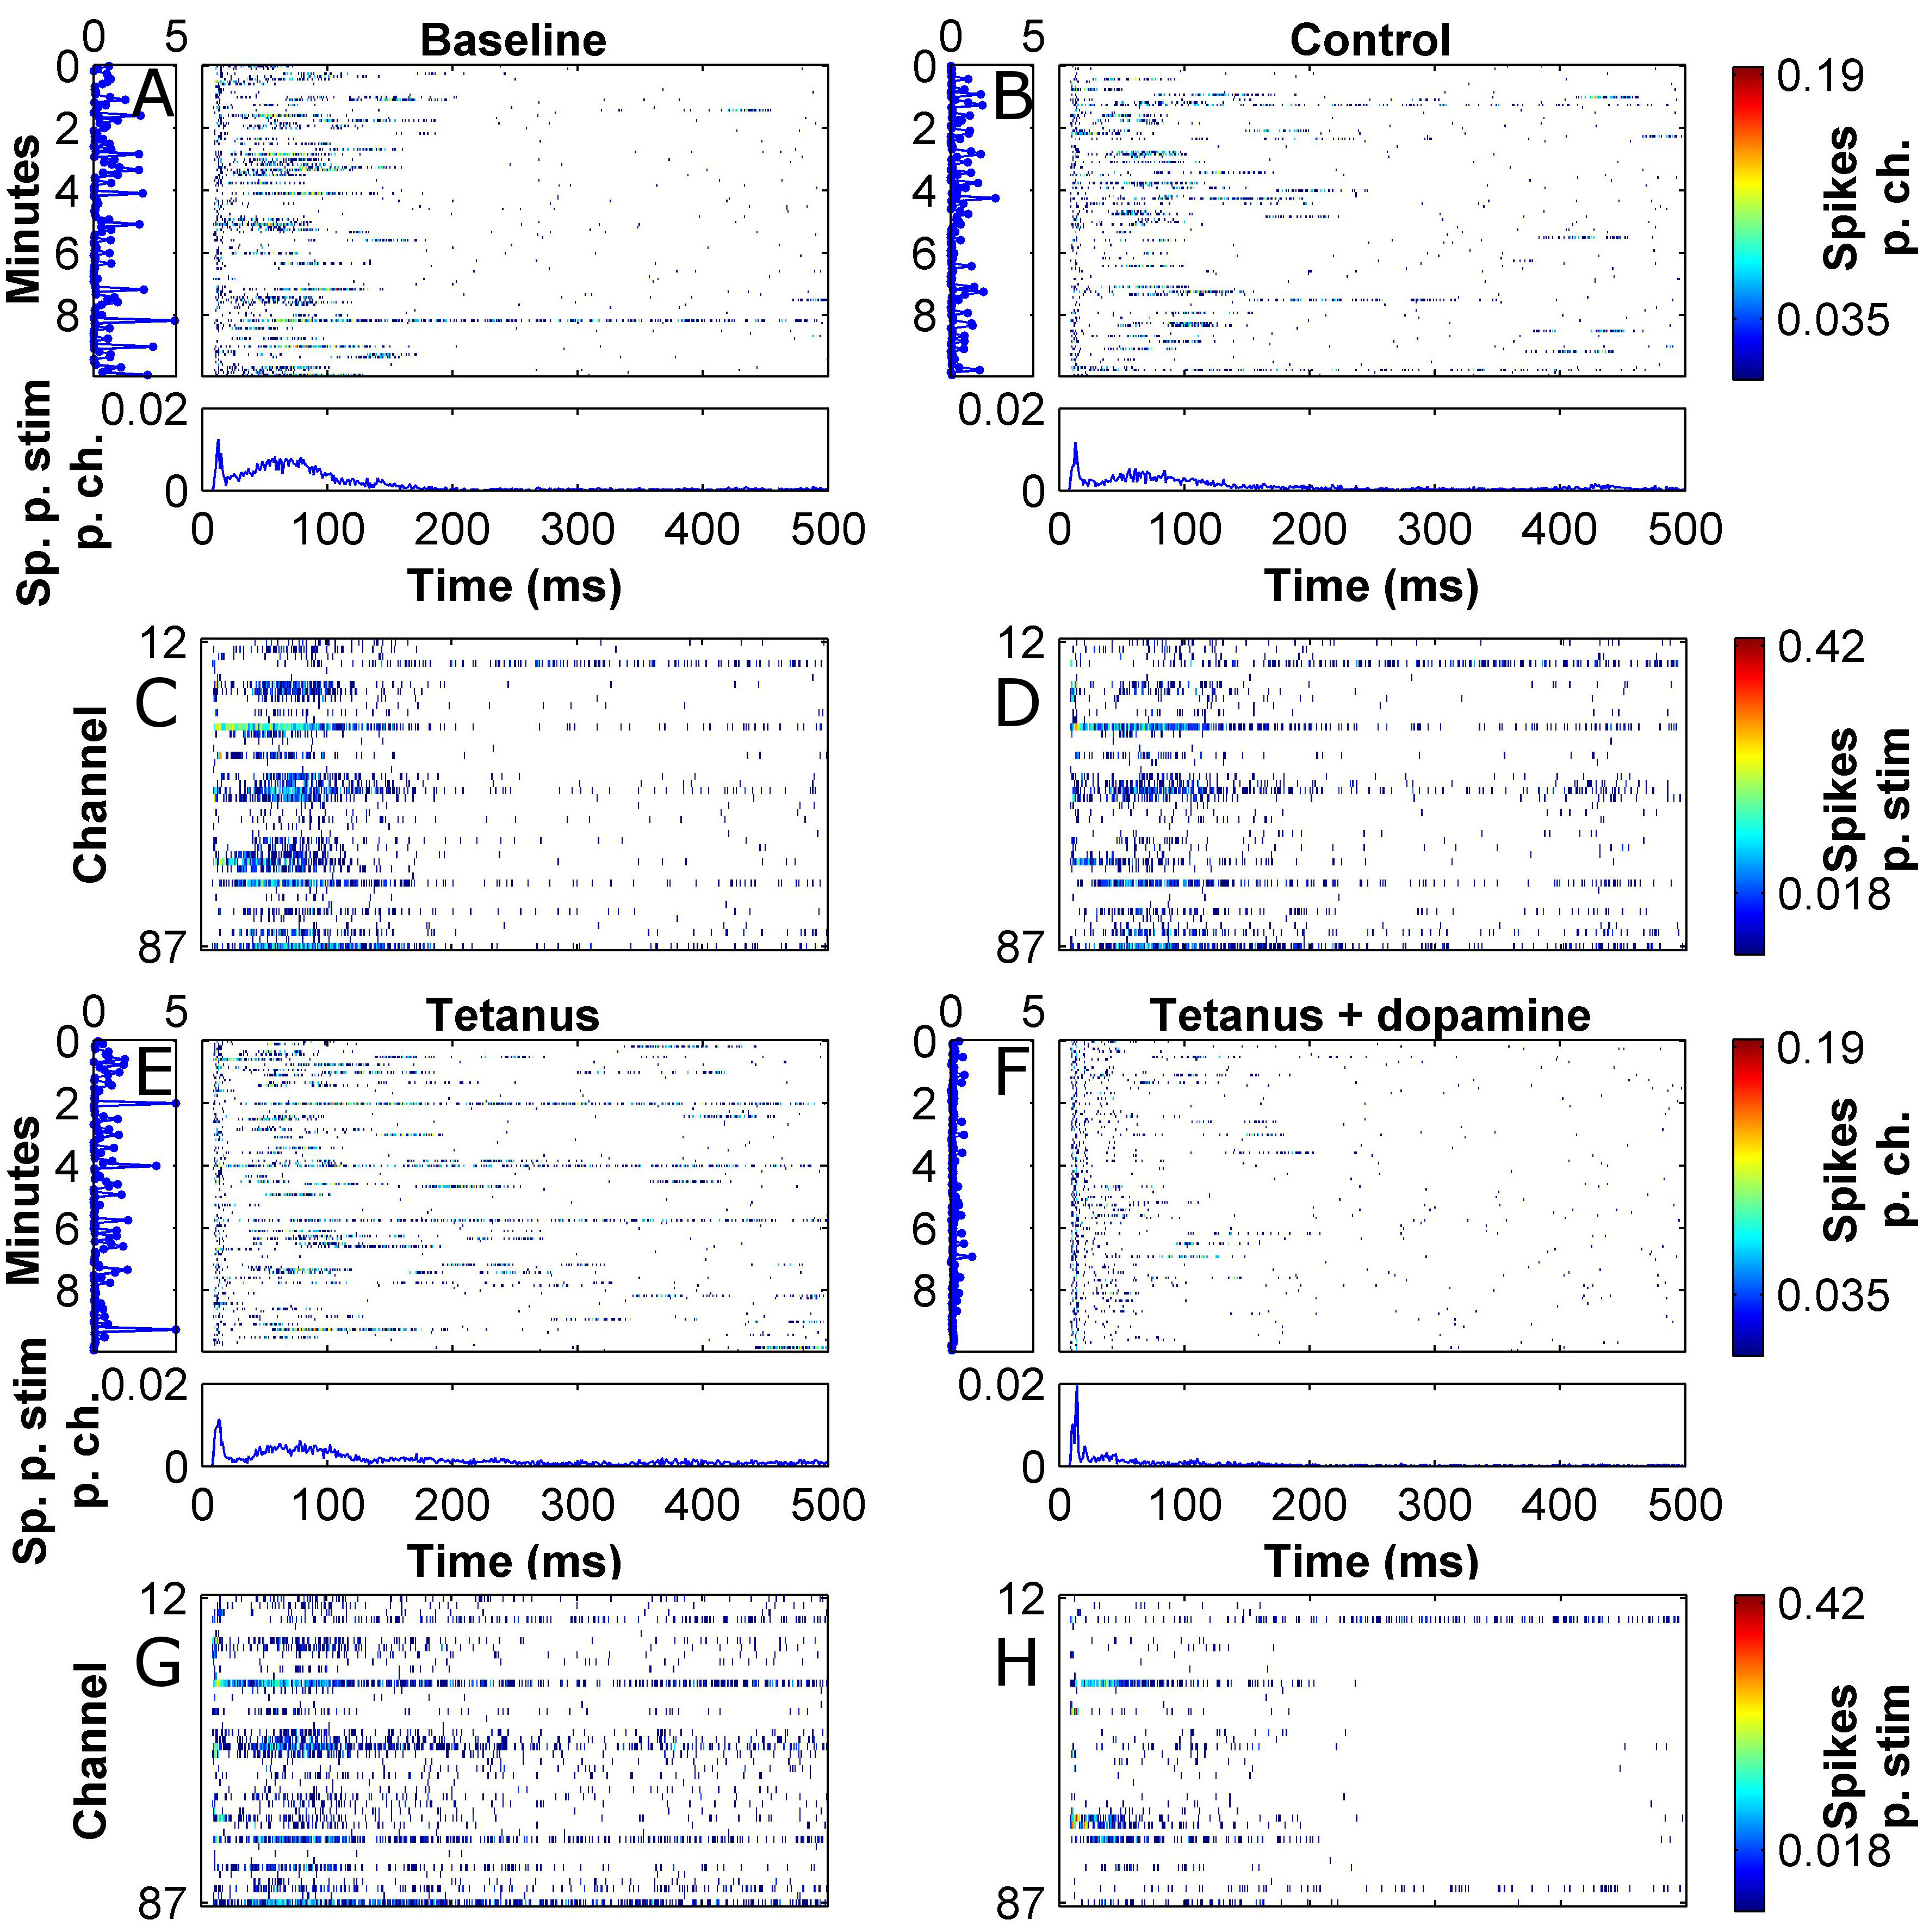
\includegraphics[width=15cm]{chapter3/figures/tetStimChange/tetStimChange.jpg}

            \caption[Example response rasters from the combined dopamine and tetanus plasticity induction experiment]{\textbf{Tetanus combined with a dopamine pulse but not tetanus alone induces a depression of evoked responses.} (A,B,E,F) Response rasters from the first stimulating electrode of each of the measurement epochs of the induction experiment. These are stimulation resolved (i.e., each line is a response to a single stimulation averaged over all the recording channels). (C,D,G,H) Channel-resolved response rasters of the same stimulation epochs. See caption of figure \ref{fig:activity:stimExample} for further details. Note an obvious decrease of evoked responses intensity following the tetanus induction in the presence of dopamine.}
            \label{fig:activity:tetStimChange}
        \end{figure}

    The tetanus + dopamine induction resulted in significantly more pronounced modifications to the evoked responses than the preceding inductions. The most obvious difference was the global reduction to the reverberating response in the PSTH. Most of the channels showed a marked decrease in intensity of responses although there were a few that actually increased. Another notable difference is that the direct response had become sharper. This global decrease in response is evident in the response maps in figure \ref{fig:activity:tetMapChange} where the number of responsive channels and their firing rate is markedly smaller after the tetanus + dopamine induction (recall that the response maps show only channels with significantly higher stimulation associated response in comparison with spontaneous activity).

        \begin{figure}[!htb]
            \centering
            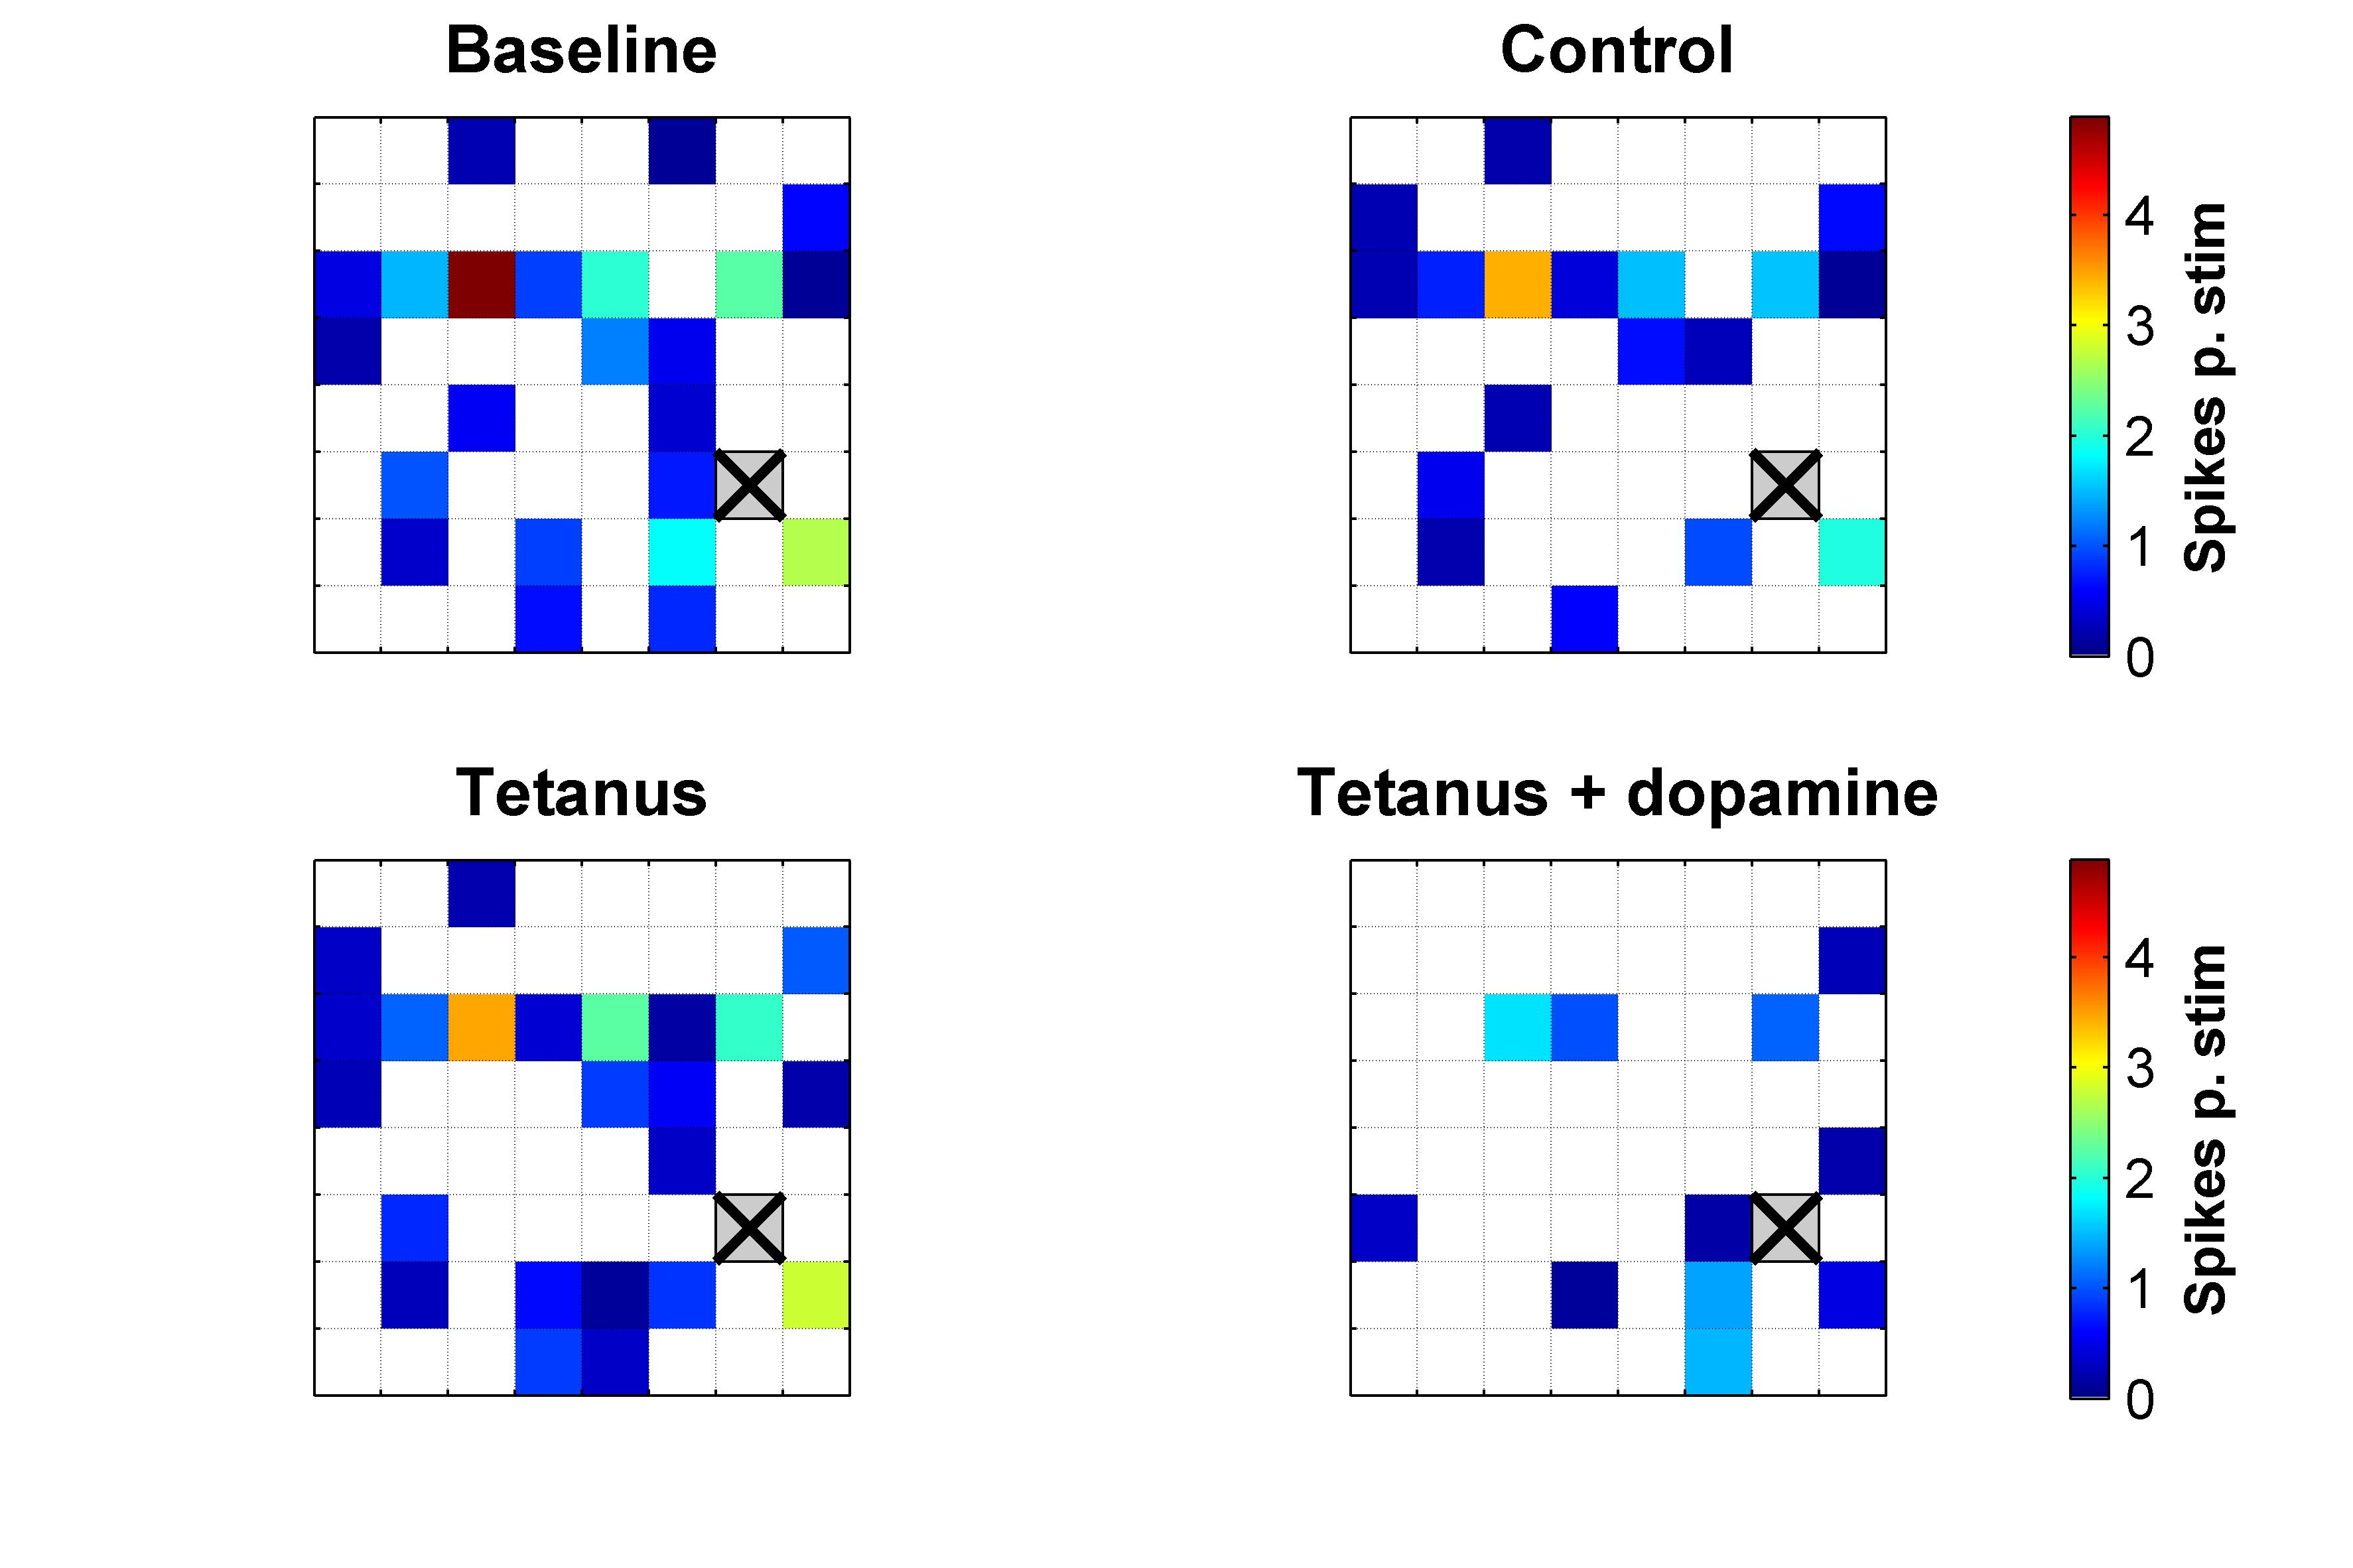
\includegraphics[width=15cm]{chapter3/figures/tetMapChange/tetMapChange.jpg}

            \caption[Example stimulation response maps for the combined dopamine and tetanus plasticity induction experiment]{\textbf{Tetanus combined with a dopamine pulse but not tetanus alone induces a reduction in the number of responsive channels.} Stimulation response maps of the same data presented in figure \ref{fig:activity:tetStimChange}.}
            \label{fig:activity:tetMapChange}
        \end{figure}


        \begin{figure}[!htb]
         \centering
         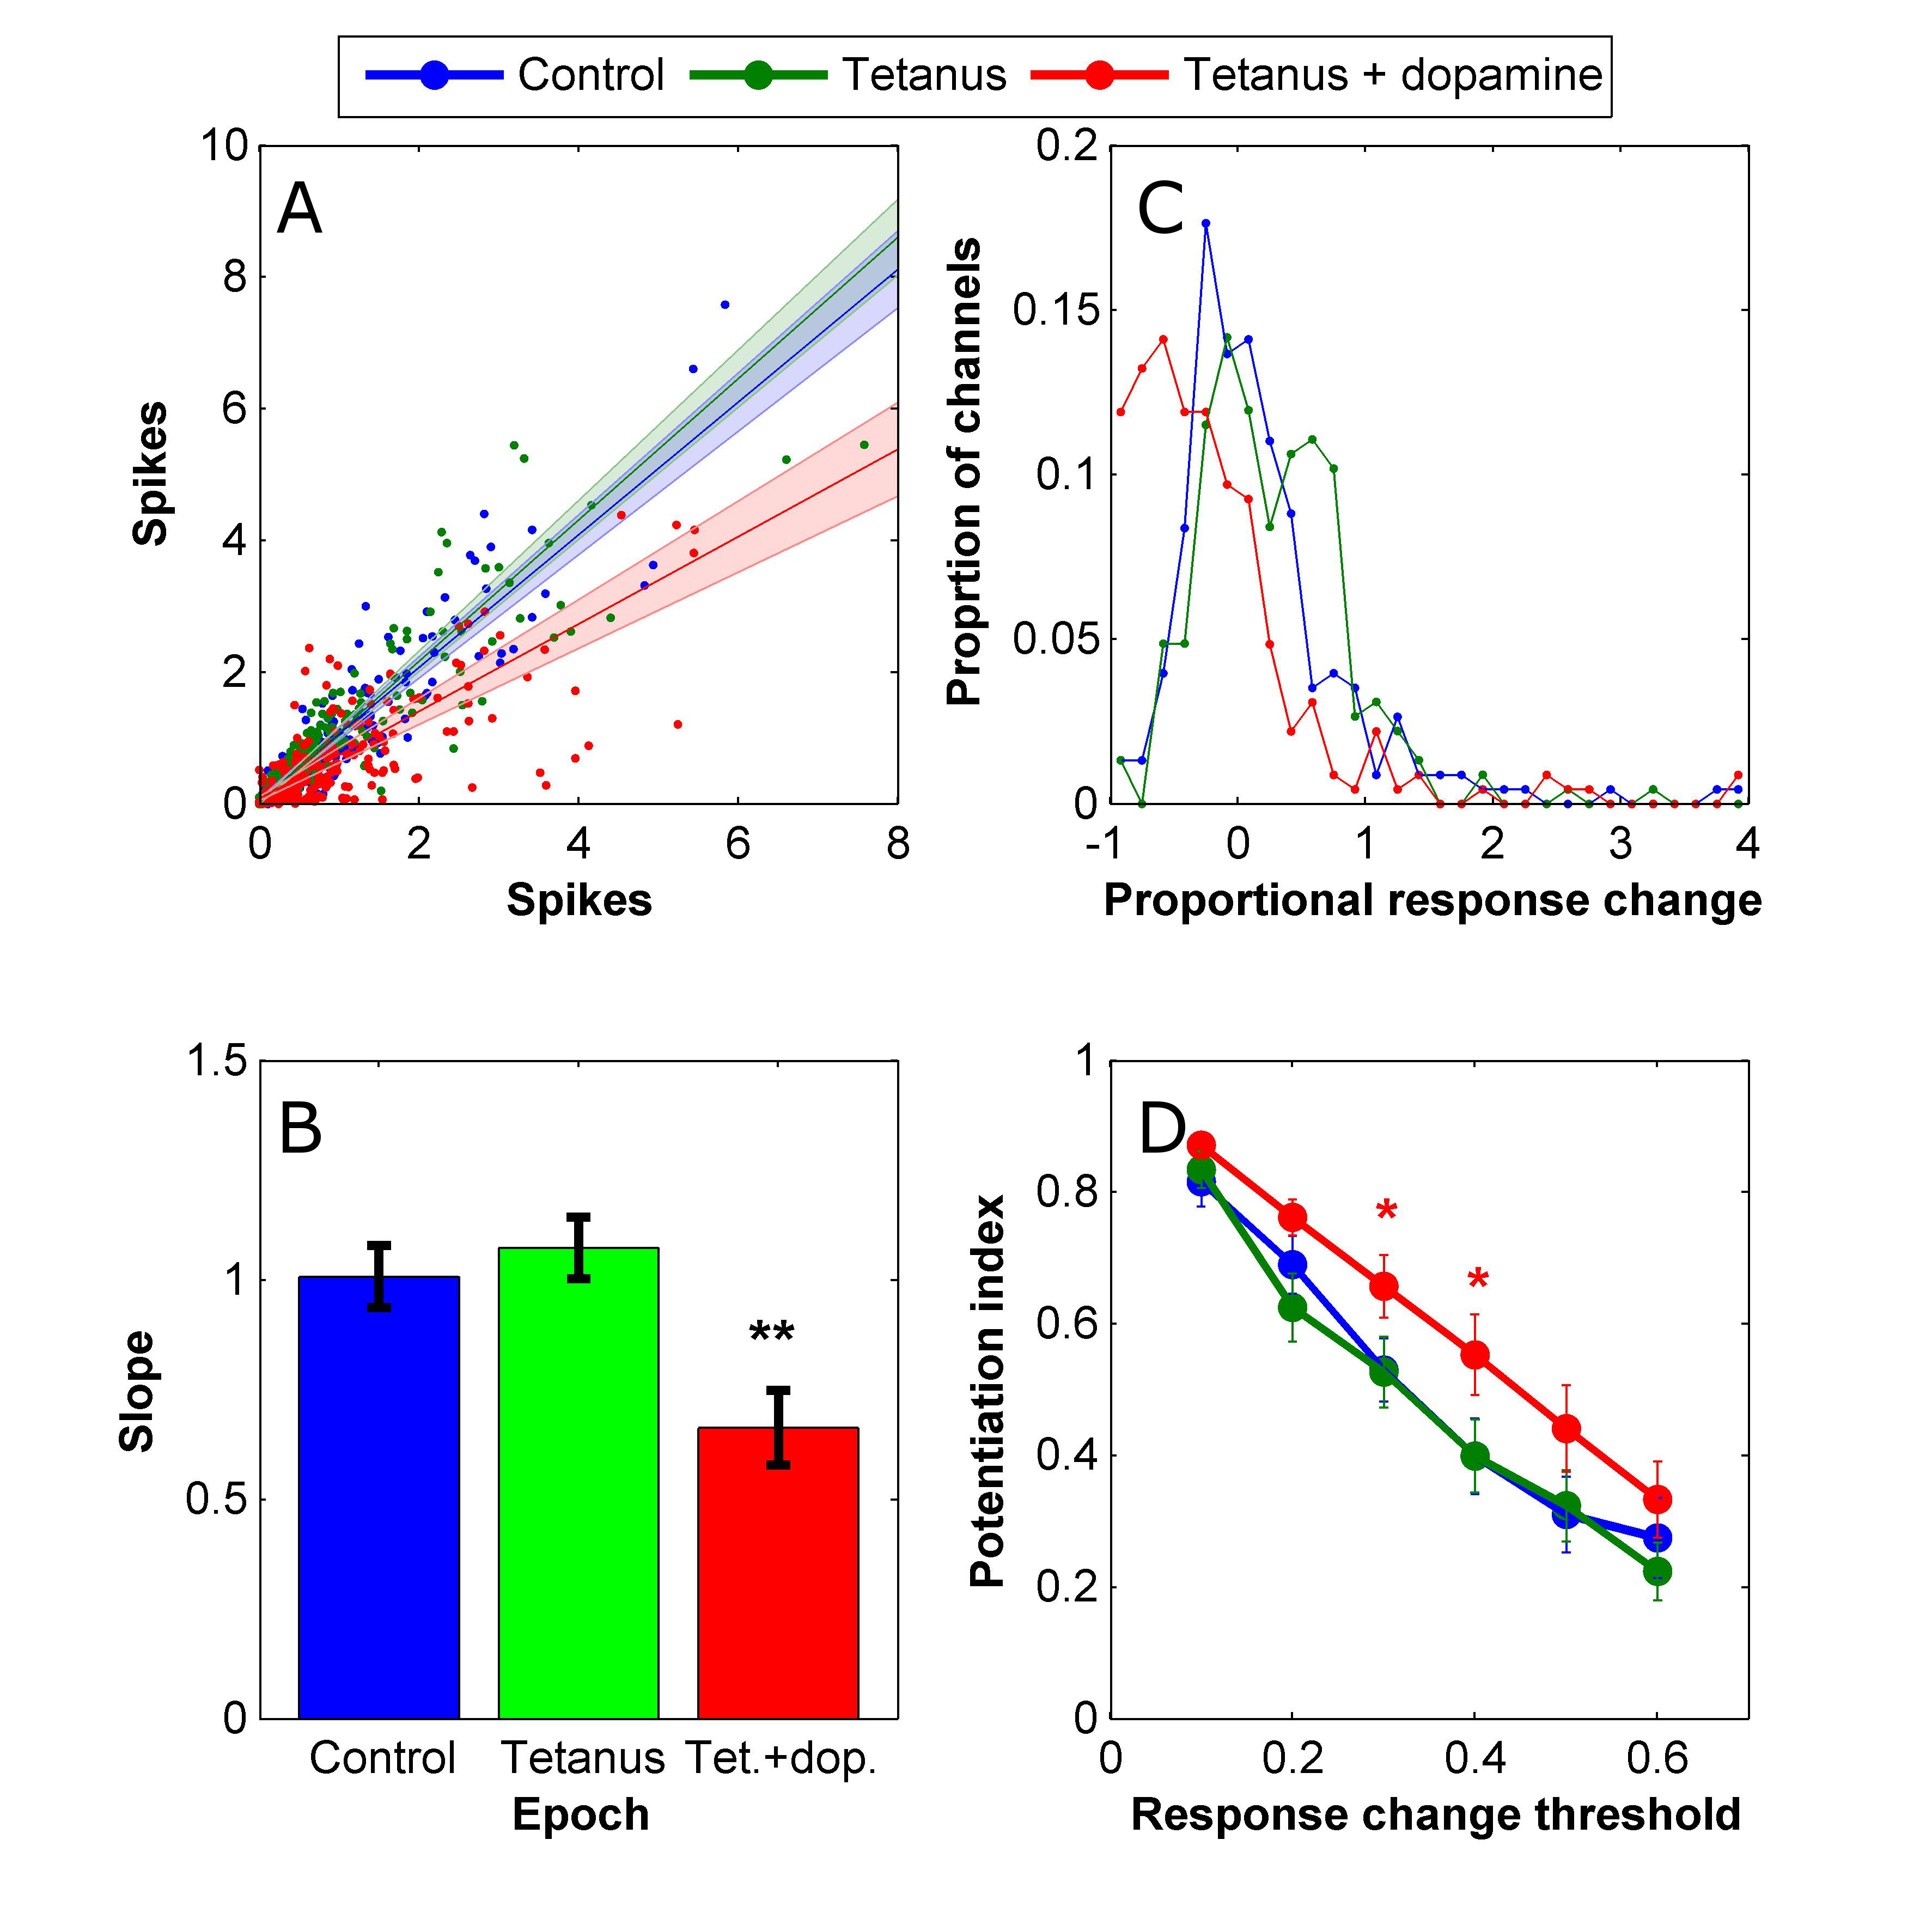
\includegraphics[width=15cm]{chapter3/figures/tetResChangeStats/tetResChangeStats.jpg}

         \caption[Statistics of changes to evoked responses in the combined dopamine and tetanus plasticity induction experiment]{\textbf{Tetanus combined with a dopamine pulse but not tetanus alone induces a depression of evoked responses.}(A) Scatter plot of pre induction vs. post induction channel responses for the 3 induction steps of our protocol. Data from all tested cultures and from all stimulating electrode are lumped. The analysis, however, considers each of these groups to be an independent data set and fits a line to each. Plotted lines and shaded areas visualize the mean and SEM of these line slopes. Data is based on 4 cultures \(\times\) 4 stimulating electrodes (n=16). (B) Comparison of fitted slopes from A. (C) Distributions of proportional changes induced in channel responses for the 3 induction steps of our protocol lumped as in A. For computation of potentiation index (PI) such distributions are generated for each data set. For each of these distributions the PI is the proportion of channels exceeding a threshold level of change. Finally, PI is computed for a range of thresholds and averaged over independent data sets (n=16 as in A). (D) Mean + SEM of potentiation index as a function of tested levels of change thresholds.}
         \label{fig:activity:tetResChange}
    \end{figure}


    Figure \ref{fig:activity:tetResChange} shows a statistical analysis of the plasticity induction experiments which closely follows the one performed in \cite{chiappalone2008network}. In essence, channel responses for each stimulating electrode were compared in a scatter plot of pre induction vs. post induction responses and a linear fit was computed (figure \ref{fig:activity:tetResChange} A-B). The slope for the 'associative tetanus' induction did not show a statistically significant difference from the one for the sham (control) induction (\(1.01\pm0.07\) vs. \(1.07\pm0.07\), 2-sided t-test, p=0.5). The slope for the induction performed in the presence of dopamine was significantly smaller, though (\(0.66\pm0.09\), 2-sided t-test, p=0.004), indicating a general depression in evoked responses (i.e., across all channels). The potentiation index analysis provided results to the same effect. This analysis is based on generating distributions of proportional changes to the channel responses before and after the induction (figure \ref{fig:activity:tetResChange} C). Potentiation index is a measure for comparing these distributions and is defined as the proportion of channels with absolute change exceeding a predefined threshold. By selecting the threshold correctly, a distinction between the distributions based on their width can be generated even if their mean is the same. In other words, this measure is designed to detect more subtle changes to the network activity that may include some of the channels experiencing large but antagonistic changes which cancel out when looking at the mean. In more common terms, one could say this is a variance or a second order measure. Since the appropriate threshold for making the distinction between the distributions is unknown, potentiation index is computed for several thresholds over the entire range of the data. It should be mentioned that the name 'potentiation index' is somewhat of a misnomer as it refers not to potentiation in the sense of strengthening but to absolute change. At any rate, applying this analysis to our plasticity induction data did not reveal any significant differences between the tetanus and control inductions. The tetanus induction in the presence of dopamine, on the other hand, showed a significantly higher potentiation using change thresholds of 0.3 and 0.4 (figure \ref{fig:activity:tetResChange} D, 1-sided t-test, p=0.034 and 0.039, respectively). This, however, is not surprising given that a general depression was observed in the preceding slopes analysis.






        \subsection{Examining changes in functional connectivity}
           Since the aforementioned analyses did not reveal any tetanus-only induced plasticity we decided to try a yet finer probing of the network activity. This is based on the functional connectivity (FC) analysis which was reported to capture plasticity in response to tetanus \cite{le2015repeated}. Mathematical details and examples for computation of functional connectivity are given in section \ref{sec:methods:FC}. In essence, the measure is based on locating peaks in the cross correlation function between channel pairs normalized to the number of spikes in the first channel. The size of the peak reflects the probability of recording a spike in the second channel following a spike in the first one at a time captured by the latency of the peak. This computation therefore results in 2 vectors, one holding peak sizes (also termed FC strengths) and the other peak latencies. Finally, differences in functional connectivity between recording epochs is measured as the Euclidian distance between the appropriate vector from the compared epochs. In our analysis we looked only at distances in the FC strengths vector because situations where the functional connectivity is lost completely (i.e., connection strength becomes 0) do not require special treatment. It has been claimed that this measure is more efficacious at detecting plasticity when computed over spontaneous activity \cite{le2015repeated} so we indeed used the spontaneous activity periods of recording in our protocol for its computation.

        \begin{figure}[!htb]
            \centering
            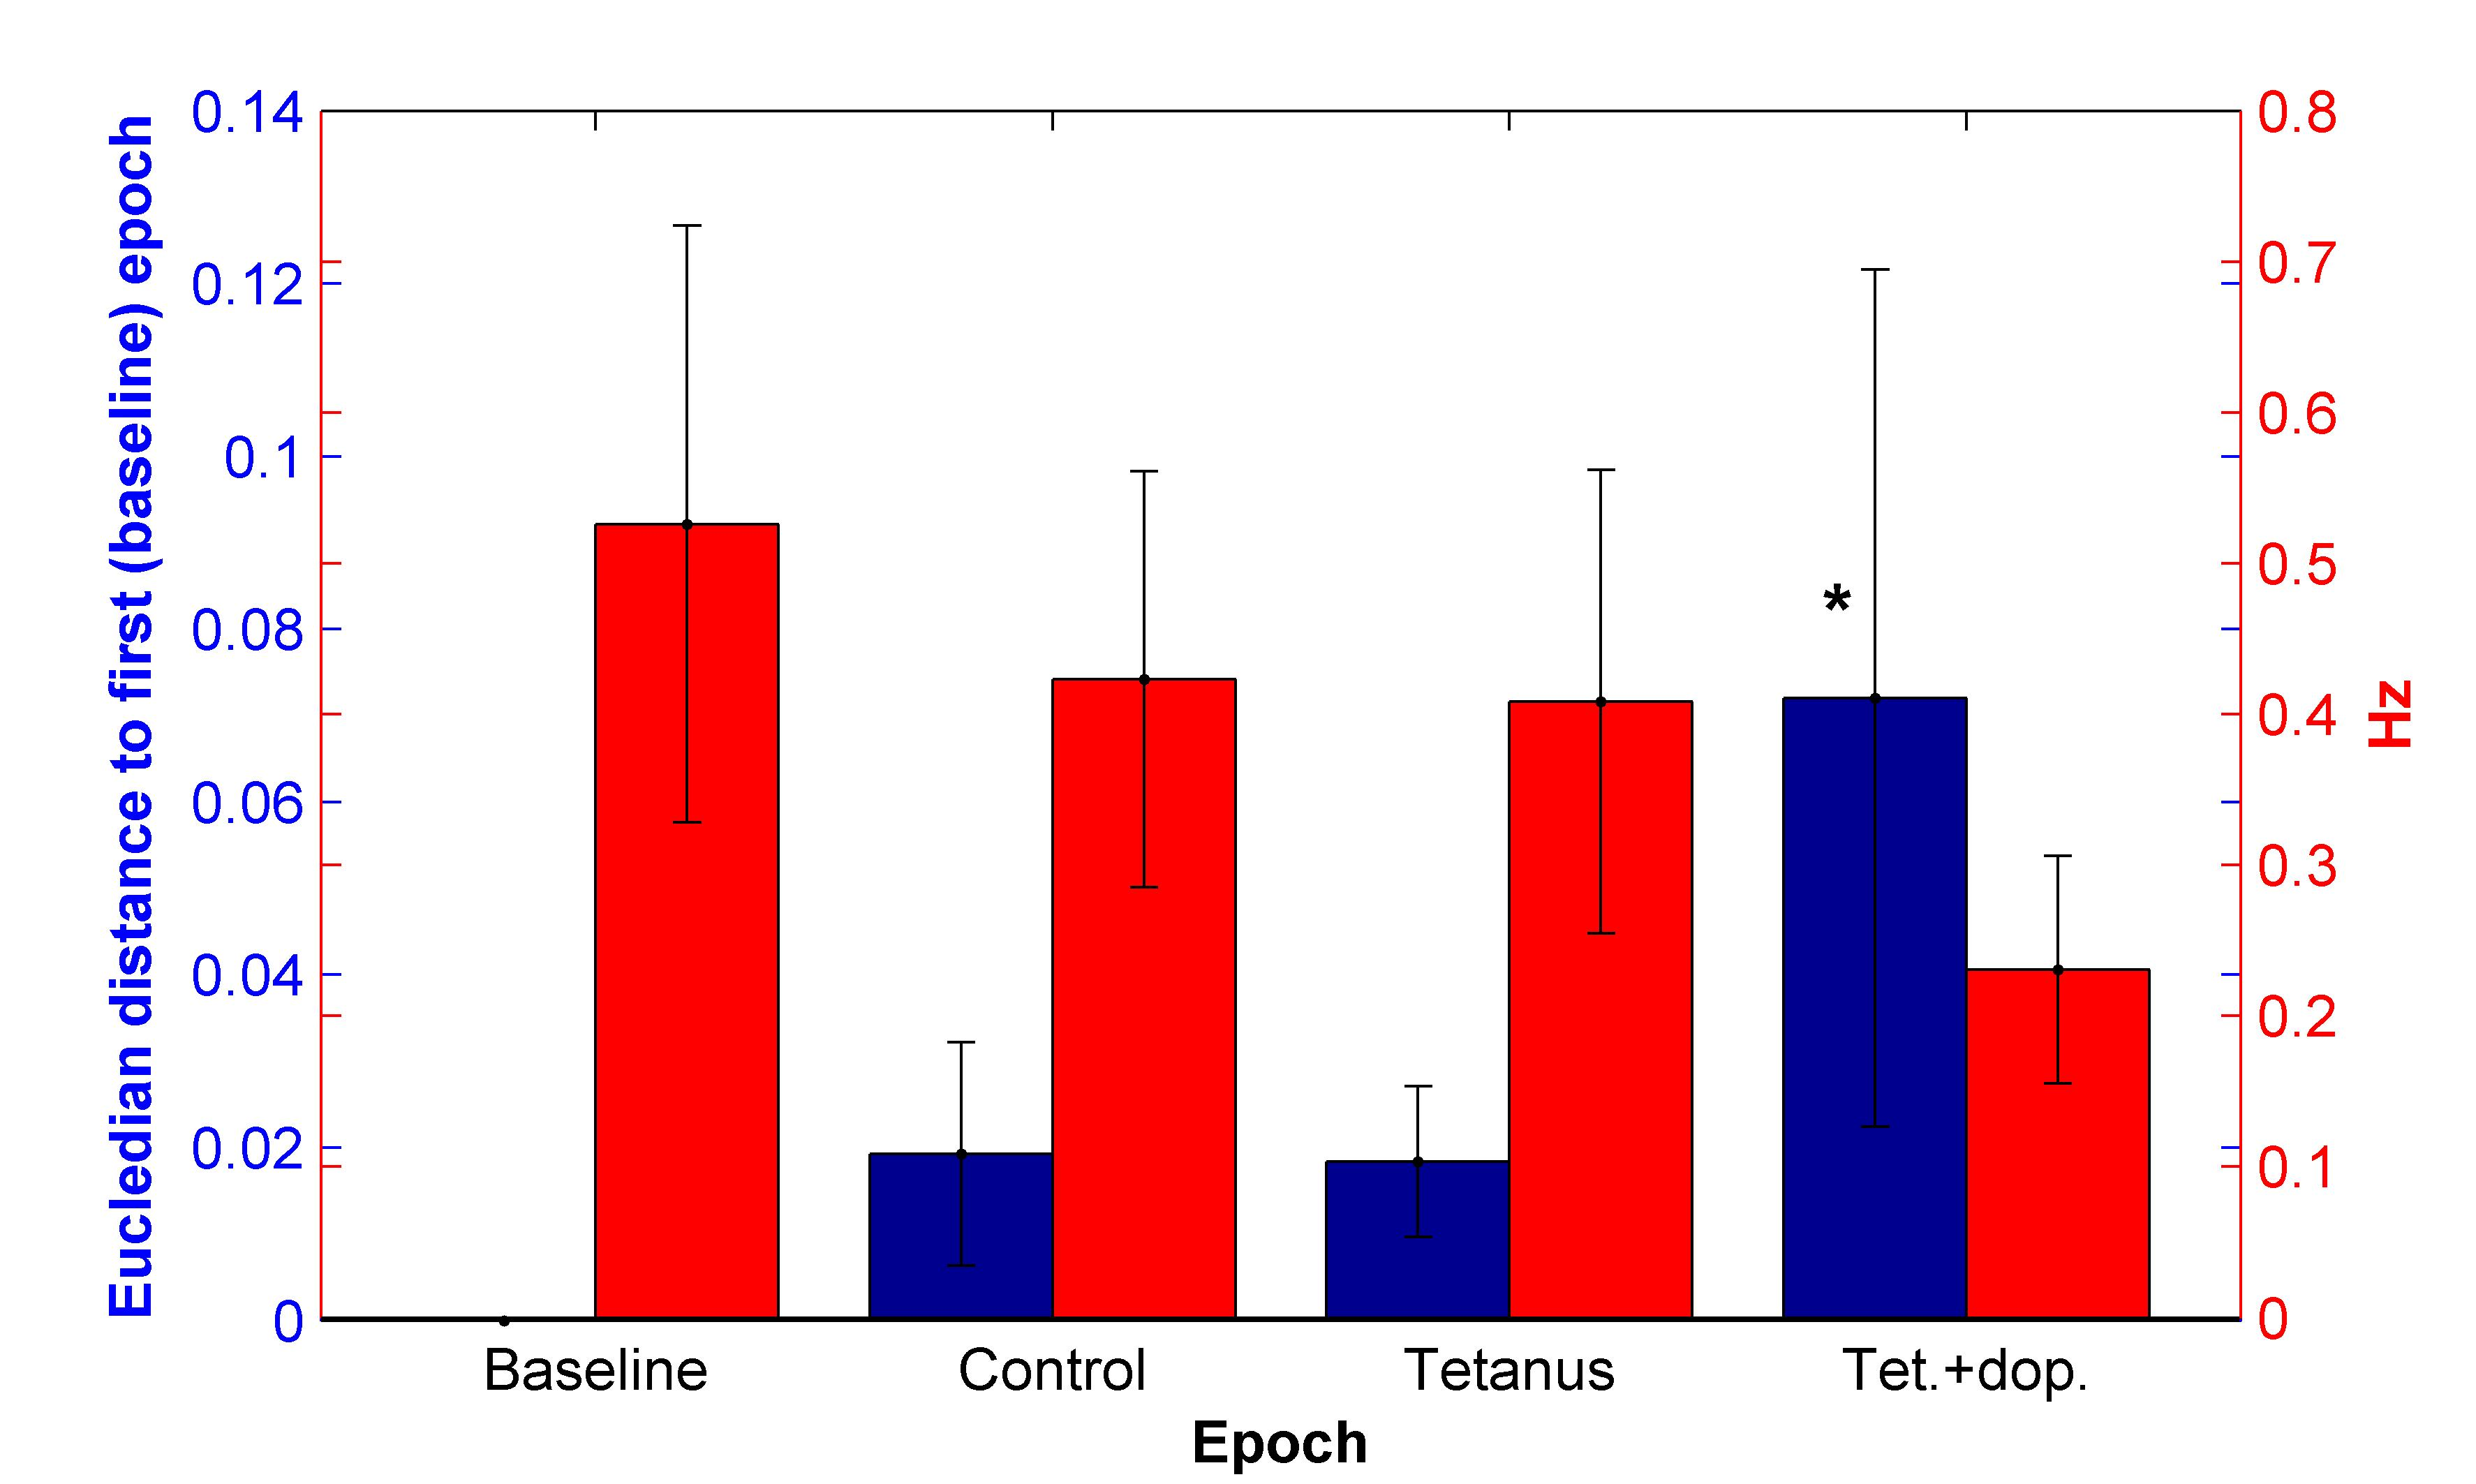
\includegraphics[width=15cm]{chapter3/figures/FCChangeStats/FCStats.jpg}

            \caption[Statistics of Change to functional connectivity and average unit firing rate in the combined dopamine and tetanus plasticity induction experiment]{\textbf{Tetanus combined with a dopamine pulse but not tetanus alone induces a change to functional connectivity as well as a decrease to spontaneous activity.} Blue bars: Euclidean distance of the functional connectivity strength vector from baseline following each induction epoch. Functional connectivity was computed based on the spontaneous activity period in each of the measurement epochs. Functional connectivity computation requires a minimum number of spikes in each of the analyzed channel pairs to generate a meaningful cross correlation function estimation (see section \ref{sec:methods:FC}) so only a subset of the possible recording channel pairs normally participate in the analysis. One of the cultures participating the the plasticity induction had to be removed as it had no channel pairs complying with the above criteria. Thus the shown data are based on n=3 cultures with 33, 10 and 179 computable functional connectivity pairs. Red bars: Mean channel firing rates in the same spontaneous activity measurement periods. This data are based on all n=4 participating cultures.}
            \label{fig:activity:tetFCChange}
        \end{figure}

           Figure \ref{fig:activity:tetFCChange} shows the changes to the functional connectivity over the different experimental protocols (measured as Euclidian distance from the baseline epoch) as well as the mean channel firing rate. The results show that the tetanus induction itself did not generate a change to the functional connectivity beyond naturally occurring fluctuations that were already observed after the control induction. A larger change was observed following the tetanus induction in the presence of dopamine which proved to be statistically significant (1-sided t-test, p=0.026). However, this change was also accompanied by a strong decrease in the mean channel firing rate which, for this data set, proved to be significant with only 90\% confidence (1-sided t-test, p=0.097). In light of this change to the averaged culture activity, the observed shift in the functional connectivity measure should be taken with a grain of salt as it was designed to reflect subtle changes to the underlying culture structure in conditions where first order statistics (such as mean firing rate) are stable.


  \subsection{Comparison between mouse and rat cultures}
    \label{sec:activity:mouseRatComp}
    As mentioned in the beginning of section \ref{sec:activity:spontActivity}, the mouse cultures posed a difficulty of a high culturing failure rate which, together with the fact that they exhibited delayed electrophysiological development raised concerns regarding their utility and ease of use. We therefore decided that, following the study performed in this chapter, rat based preparations would be used for the remainder of the Ph.D work. Here we outline a brief pilot study to compare our rat based preparations with the mouse based ones and assert that the former shows an electrophysiological profile in par with the literature. In order to compare the functional development of mouse based and rat based cultures we recorded spontaneous activity from a set of rat cultures, prepared using a protocol identical to the mouse ones.

       \begin{figure}[!htb]
            \centering
            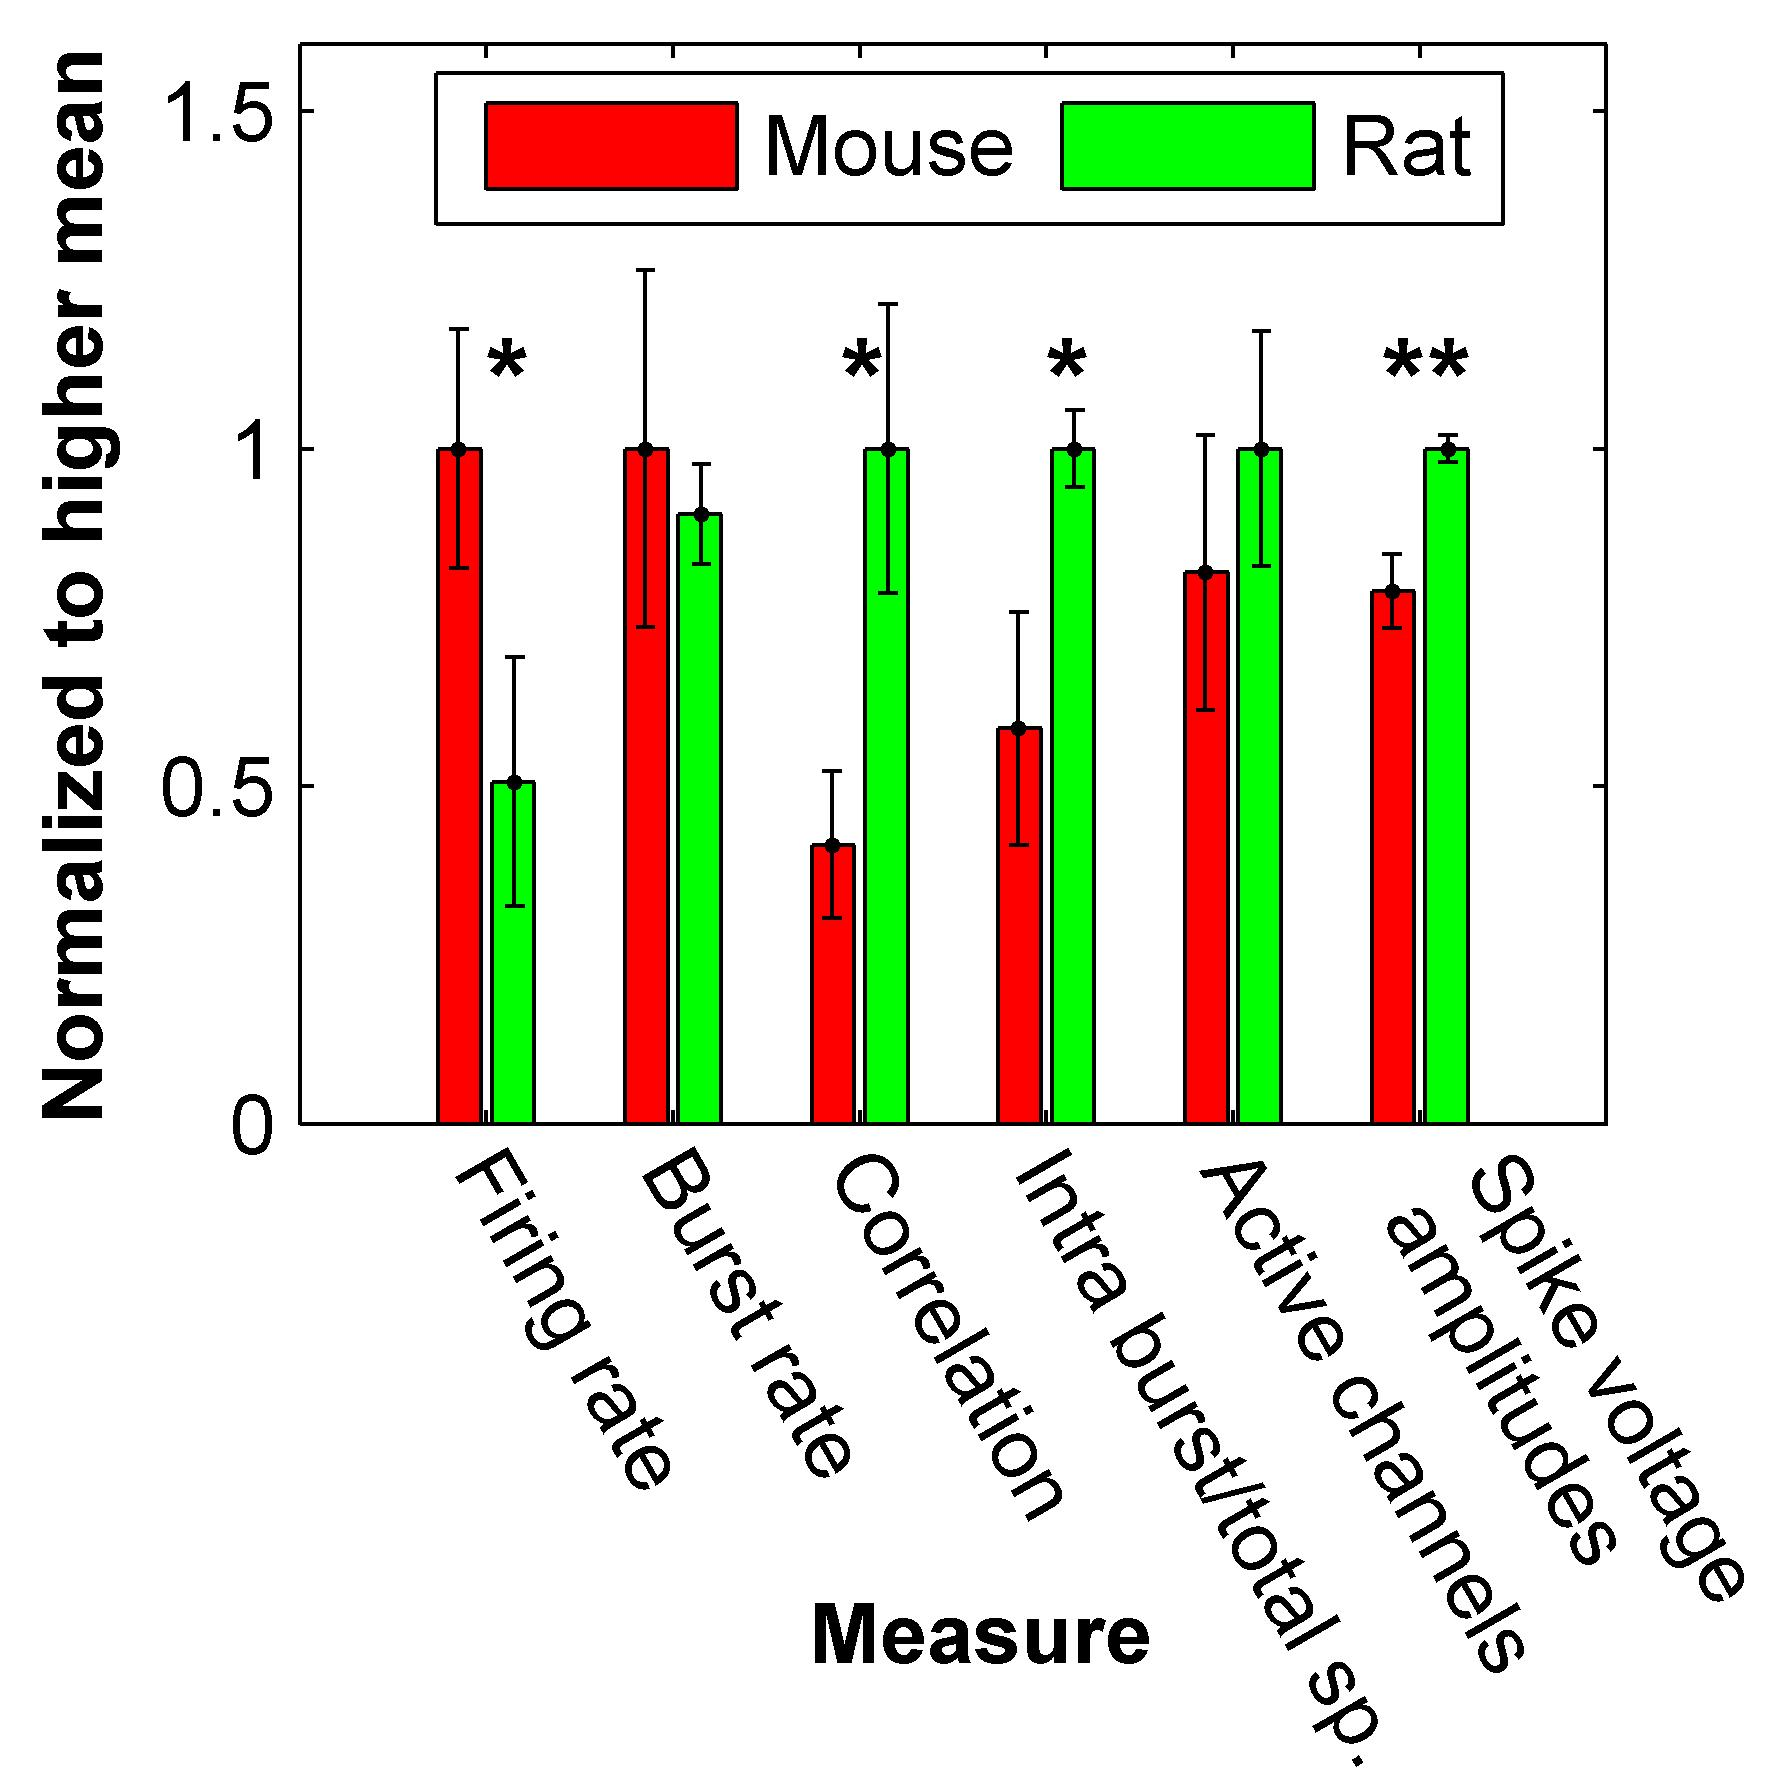
\includegraphics[width=7.5cm]{chapter3/figures/mouseRatComp/ratMouseComp.jpg}

            \caption[Comparison between spontaneous activity in mouse and rat based cultures]{\textbf{Rat cultures show increased correlation as compared to mouse cultures at the same age.} Six measures are considered and are normalized to whatever mean is higher amongst the two compared groups. *, ** indicate statistical significance of the difference between the groups at levels of confidence of 95\% and 99\%, respectively. Mouse statistics are based on n=5 cultures and rat statistics on n=4 cultures. Culture ages at the time of recording were selected so that both groups had the same mean age of 19.5 days \textit{in vitro} (range \(15-23\) DIV for rat and \(18-20\) DIV for mouse).}
            \label{fig:activity:mouseRatComparison}
       \end{figure}

    Figure \ref{fig:activity:mouseRatComparison} shows a comparison between rat based and mouse based cultures at the same age \textit{in vitro} for several activity and synchronicity measures introduced earlier. A particularly pronounced difference was observed in the closely related measures of correlation and ratio of intra-burst to total activity both of which showed a significantly higher values in the rat cultures (1-sided unbalanced t-test, p=0.017 and 0.039, respectively). These differences demonstrate that mouse cultures exhibited more uncorrelated activity as compared with their rat counterparts. This reiterates the observation discussed in the previous section that the mouse cultures show delayed synaptic development.

    Another observed difference is that the mouse cultures showed a significantly higher average unit firing rate (one sided unbalanced t-test, p=0.048). This result could be another manifestation of the rat neurons being more attuned to the synaptic drive from the network but is harder to interpret. In any case, the mean values for both preparations types (\(1 Hz\) and \(0.5 Hz\) for mouse and rat, respectively) are within the rat literature range (\(0.4-1.5 Hz\)).

    Both preparations showed a nearly identical burst rate of about 15 minute\textsuperscript{-1}. The burst rate measure is different to the correlation and activity ratio measures in that it counts synchronized events but is indifferent to activity outside such events. This in contrast to the correlation and intra-burst to total spikes ratio measures which are sensitive to activity both inside and outside the bursts. The fact that the reduced synaptic coupling in mouse cultures does not affect the burst rate suggests that the this measure is strongly related to the general excitability and not just to the synaptic development.

    Finally, the spike amplitudes measure shows the mean of peak voltage in the recorded extracellular spike waveforms across all mouse and rat recordings (see section \ref{sec:methods:MEARecording} for example waveforms). Surprisingly, we found a significant reduction in peak voltage for the recording from mouse preparations as compared to the rat preparations. This indicates that the two types of neurons are different in their excitability properties and that, possibly, mouse neurons express a lower density of voltage dependent ion channels.

    In summary, the comparison confirmed that the mouse cultures are delayed in synaptic maturation as compared to rat cultures and thereby display reduced correlations at the same age \textit{in vitro}. As far as these results can corroborate, our rat based preparations present all the features and developmental time course that have been described in literature and will therefore will be selected for the work carried out in the following chapters.


    \section{Chapter conclusion}
    The main purpose of this chapter was to establish the standard neuronal culture on MEAs model system together with the accompanied Matlab analysis and show that the cultures are healthy and exhibit the diverse electrophysiological characteristics which have made them a successful neuroscience model system. Indeed distinct stages of development of network activity were clearly observed. These consisted of initial uncorrelated but widespread firing patterns corresponding to neuronal maturation followed by an increase in correlations and rate of synchronized events which indicate that the synapses are maturing. Further examination of the data revealed evidence for other neurobiological processes that have been described in culture. These included homeostasis of activity rates, existence of strongly intra-connected subnetworks and a gradual temporal narrowing of the synchronized events which has been attributed to a delayed maturation of the GABA neurotransmission system as compared to the glutamatergic one. These processes have not been studied here in depth but are taken as evidence that our cultures are healthy and in par with the literature. It is important to note that these observations have been made on mouse cultures which have been seldom used in the MEA context. The provided data thus establish their usability even though certain difficulties were also reported which made us eventually switch to using rat cultures.

    The final undertaking of this chapter was to explore a protocol for phasic application of dopamine using manual pipetting. We modified a common plasticity protocol to include a step where dopamine is applied exclusively during the tetanus induction step (through manual pipetting and subsequent washing). Without any dopamine, we were not able to induce a change in the culture activity, despite reports to the contrary in the paper from which the protocol was adapted. This should not come as a surprise as the literature is controversial in this regard and should just serve as a demonstration that further work is required for these systems to serve as a useful model of plasticity. Following a tetanus induction which was performed in the presence of dopamine a significant depression was observed in the evoked responses which were measured up to an hour following the induction. The spontaneous activity was also depressed but to a lesser extent. On one hand this could demonstrate an enablement of LTD by the dopamine. The fact that this effect is present after the dopamine had been removed strengthens the possibility that this is a plasticity effect rather than a result of direct interaction of the cells with the agonist. Indeed a similar experiment had been performed in cortical slices and produced very similar results \cite{otani1998dopamine}. On the other hand, it is also known that in neuronal culture the mere action of media replacement drastically reduces activity (this  will be made very clear by the results of chapter \ref{chap:activityAndFlow}), an effect the could last several hours. Additionally, the presence of dopamine itself is known to have an inhibitory effect in the cortex regardless of plasticity \cite{gu2002neuromodulatory,gonzalez2001dopamine} and it is hard to rule out the option that a small concentration of the agonist is still present after the washing step and contributing to the observed effect. Under the constraints of the current bath application methods, it is impossible to run a dopamine pulse without these impinging effects. Undoubtedly we could quantify them by using a set of control experiments but we cannot eliminate them.

    To summarize, these dopamine pulsing results are promising in that they suggest a potential for dopamine to enable plastic behaviour in culture. However, this notion wasn't fully proven due to uncertainty about the effects of media replacement and of temporary interaction of dopamine with the neurons. This highlights the need for a precise solution exchange system whereby dopamine can be applied with high spatio-temporal precision and without change to other extracellular ingredients which could interfere with the activity. Such a system would allow interrogation into the fine temporal details of the phasic dopamine and volume transmission processes in general far beyond what was demonstrated in the above-described work. The following chapters in this Ph.D thesis will describe the development and establishment of a microfluidic based rapid solution exchange system where the drug delivery is rapid, precise and decoupled from other changes to the extracellular chemistry.

%\chapter{Viability of neuronal cultures in microfluidic devices in static conditions and under steady flow}
\label{chap:devicesAndFlow}


\section{Introduction}
\label{sec:devices:introduction}
As outlined in section \ref{sec:introduction:objs} the purpose of this Ph.D work is to produce a model for phasic neuromodulator signalling by generating rapid agonist transients onto an entire neuronal culture. This is to be achieved using the interface shifting method in microfluidic devices (see section \ref{sec:introduction:mufdDrugDelivery}). As we will show, successfully applying this method to generate transients at time scales mimicking phasic neuromodulator signalling involves rapid flow rates in the order of \(1\frac{mm}{s}\). Previous microfluidics work involving primary neurons used such rapid flow rates but just for short experiments lasting between minutes to 2 hours at most \cite{biffi2012microfluidic,morel2012amplification,wang2008microfluidics,pearce2005integrated}. Studies showing long term neuronal culture development under flow used much reduced flow rates where the convective forces were comparable to diffusion \cite{choi2013neurotoxic,millet2007microfluidic,park2015three,kumamoto2015effects}. Thus to avoid the complexity involved in getting neuronal cultures to survive long term under rapid flow we elected to follow an experimental paradigm whereby the cultures were initially grown in microfluidic devices in static conditions. After reaching maturity they were subjected to flow only for the duration of the experimental session. The first part of this chapter is dedicated to development of a protocol for long term culturing of primary rat neurons in microfluidic devices. As reviewed in section \ref{sec:introduction:mufdNeuroscience}, this type of protocol is prevalent in the literature but the configuration of our devices, which were designed with the interface shifting method in mind, required specific adaptations.

An important part of the our experimental design is for the culture to be of restricted size (i.e., a microculture). This is necessary, firstly, because the interface shifting routine involves having a small proportion of the microfluidic channel area chronically exposed to the agonist, even between transients (see section \ref{sec:introduction:mufdDrugDelivery}). Thus to avoid such chronic drug exposure, the culture needs to be located entirely outside the chronically exposed area. Secondly, it is important to note that an agonist pulse in the interface shifting method actually takes the form of an agonist wave travelling along the long axis of the channel. This means that, depending on the flow rate and the geometry of the culture, cells at different locations along the channel may experience the drug at different times following the pulse command. In phasic neuromodulator signalling, the agonist molecules are secreted from nerve terminals that innervate the entire volume of the target tissue. Consequently, a neuromodulator pulse involves an approximately synchronous increase of agonist concentration over the entire innervated tissue followed by a decrease in concentration as the agonist molecules get locally re-uptaken \cite{arbuthnott2007space}. It is important to note that, due to inhomogeneities in the spatial distribution of the innervating neuromodulatory fibers, different parts of the tissue still exhibit some delays in exposure to the agonist depending on their proximity to neuromodulatory synapse clusters. Nevertheless, these delays are small compared to the time scales of the global pulse \cite{arbuthnott2007space,venton2003real}. Because of the functional importance of timing in the neuromodulator signalling, it is essential that the microfluidic model does not exhibit increased delays in arrival of the agonist to different parts of the culture as compared to the \textit{in vivo} tissue. To achieve the right timings, the flow speed and culture size need to be selected so that the drug traversal time across the culture matches the delays in the modeled tissue. Thus, the ability to control the culture size is crucial and the second part of this chapter will describe a method for generating microcultures which harbour small specific areas of the channel by utilizing microwells. The viability of these microcultures will be analyzed to establish their usability.

A final important topic that will be covered in this chapter is that of neuronal viability under rapid flow. Primary neurons are considered to be highly sensitive to shear stresses. Since this system is developed with long term plasticity in mind it is important to make sure that the culture is kept viable and functional for at least several hours under the applied shear stresses. It is also important to take into account that a functional neuronal tissue employs a large number of intrinsic volume transmission processes which comprise controlled secretion and uptake of active substances into the ECM (reviewed in section \ref{sec:introduction:volTrans}). These substances include neurotransmitters, hormones, neurotrophic and growth factors and are generally termed conditioning factors. Rapid flow is likely to interrupt these processes by changing the concentrations of the conditioning factors or their spatial distributions. Since microfluidic flow has been scarcely used with primary neuronal cultures the flow rate limits have not been established and it is currently unclear what is the impact of each of the above-mentioned factors, shear stress and conditioning removal, on the culture viability. To characterize the effect of these factors we performed a viability assay under flow with a range of flow rates and media conditioning levels.

\section{Long term neuronal cultures in microfluidic devices}
    \subsection{Development of protocol}
    \label{sec:devices:protocolDev}

    This section outlines the development of a protocol for long term culturing of primary hippocampal neurons in microfluidic devices. Long term culturing of cortical and hippocampal neurons has been established for over 30 years \cite{brewer1993optimized,romijn1984towards,ray1993proliferation}. Recently, there has been an emerging use of microfluidic devices to culture neurons with increased control over the topology and to access specific neuronal compartments \cite{park2006microfluidic,park2013advances,gross2007applications}. Nevertheless, neuronal cultures are infamous for their sensitivity to subtleties in the preparation technique and the materials that come in contact with the media or the cells and often require specific adaptations for the specific lab / application \cite{kaech2006culturing,millet2007microfluidic}. We first established the required device geometries for our application and the conditions required for long term neuronal culturing in them.

    Figure \ref{fig:devices:basicDimensions} shows the dimensions of the devices used in this study. The dimensions were selected so that, given the volumetric flow rates allowed by our flow system, a flow speed would be produced that is compatible with the desired agonist exposure times. Thus the main channel width was \(1.5 mm\) and the height was \(65 \mu m\) giving a cross section of \(\approx 0.1 \mu m^{2}\). Using a flow rate of \(100 nl/s\) gives an averaged flow speed of \(1 mm/s\). Assuming that the long dimension of the culture would be less than a millimeter and that the culture would be positioned less than a millimeter from the agonist port then the agonist should reach the culture within a second and clear it a second later, which is the correct order of magnitude for neuromodulator phasic signalling \cite{venton2003real}. These initial calculations indicate the required channel geometries. Detailed testing of solution exchange under flow are reported in chapter \ref{chap:microculturePulses}.

    The devices were bonded to glass cover slips using plasma bonding (see section \ref{sec:methods:bonding} for details and more illustration of the assembled devices), oven sterilized, and then subjected to PLL surface treatment as detailed in section \ref{sec:methods:surface}.

    Due to the need to interface with a flow system, the microfluidic devices used in this work were made with biopsy punched ports of \(\approx 0.8 mm\) diameter which allow connection to the flow tubing by simple pressure fitting. This design contrasts with standard neuroscience oriented microfluidic devices where the ports are typically of \(8 mm\) diameter (e.g., \cite{park2006microfluidic,robertson2014chemically,millet2007microfluidic}). In these standard devices the seeding proceeds through pipetting of the cell solution into the ports and allowing the cells to flow through the channel (flow is enabled by controlling for a differential media height across the inlet and outlet ports). In the case of these standard devices, the ports function as de facto reservoirs by holding a significant volume of media (\(400 \mu L\) each) and therefore protect the device from dehydration and serve as a source of nutrients. Due to the smaller port size in our devices, plating was performed by injecting the cells into the inlet port using a gel loading tip. The volume of injection was selected to be larger than the internal volume of the device so as to fully flood it with cells. The devices used here had an internal volume smaller than \(1 \mu L\) (figure \ref{fig:devices:basicDimensions}) and the injection volume was \(2 \mu L\). After completion of the injection the cells were left suspended in the channel volume and were allowed to settle down in the incubator. The lack of flow following the cell injection made this protocol more consistent than the flow based seeding in standard devices. In those cases too strong of a flow ends up in having most of the cells flow through the device without settling and therefore in inconsistent seeding densities. On the other hand, a down side to our design is that due to their smaller diameter, the ports in our devices only hold about \(2.5 \mu L\) of media each and therefore cannot effectively fulfill the role of media reservoirs.

    The following subsections will outline the major steps taken during the development of the protocol to circumvent the issues encountered along the way. The development of the protocol was an iterative process, where pragmatic progress was prioritised over statistical testing of each step. The goal was to identify a strategy for reliably seeding channels with viable neurons that was reproducible and met the design criteria needed for rapid delivery of neuromodulators. Accordingly, a detailed analysis of the factors determining neuronal viability was not carried out but is presented in the form of examples and heuristics for the benefit of scientists wishing to use these techniques.

      \begin{figure}[h]
           \centering
            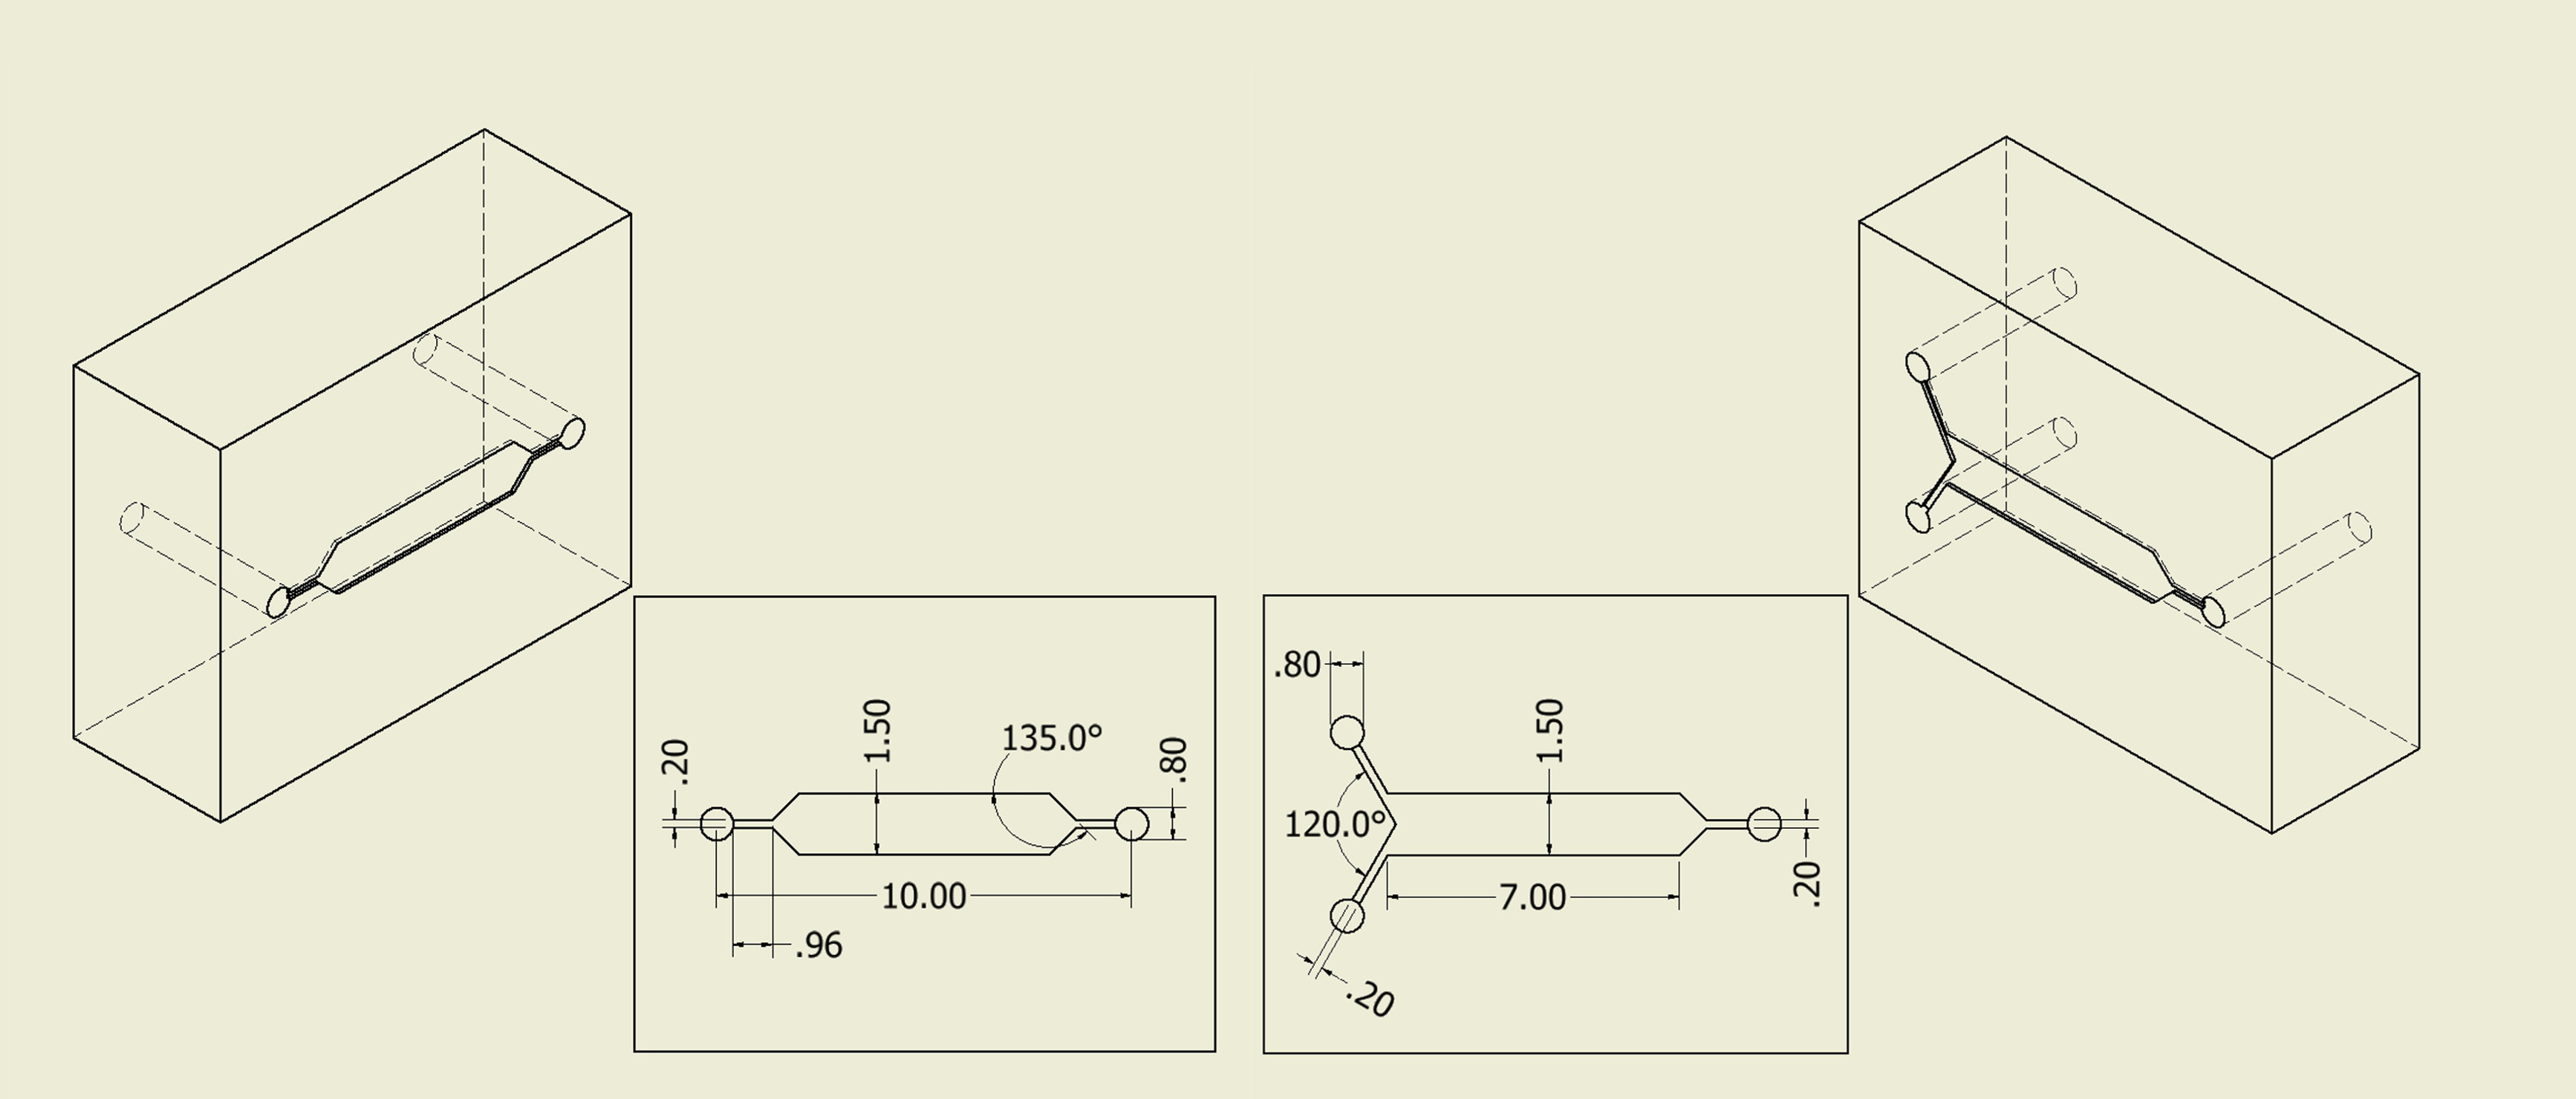
\includegraphics[width=14.5cm]{chapter4/figures/channelDimensions/dimensions.jpg}
            \caption[Schematics of the standard single layer microfluidic devices]{\textbf{Schematics of the standard single layer microfluidic devices.} All measurements listed in mm. Standard single layer microfluidic channels used in this section comprised both 2-port and 3-port (y-shaped) configuration.}
            \label{fig:devices:basicDimensions}
     \end{figure}



        \subsubsection{Evaporation and surface chemistry considerations}
        The initial incubation configuration explored was to apply a \(200 \mu L\) drop of media to the top of the PDMS surface to act as a media reservoir from which nutrients are exchanged and to preserve the aqueous environment. To minimize evaporation, the devices were further kept in a closed petri dish next to a dish with \(1 mL\) DDW. The petri dish was kept in a humidified CO\textsubscript{2} incubator (Figure \ref{fig:devices:osmIssue} A). The initial configuration also incorporated a 30 minute incubation with PLL solution as surface preparation. Cultures seeded in this configuration did not develop long term. The cells were initially healthy and adhered to the surface but the adhesion was non-uniform and by 5 days \textit{in vitro} the cultures degenerated (figure \ref{fig:devices:osmIssue} C-D). The main issue associated with this device configuration was that evaporation from the media on top of the devices was causing a rapid increase in the media osmolarity at a rate intolerable to the cells. We quantified this effect by measuring the osmolarity (Osmomat 030, Gonotec) of the media on top of 15 such devices after an overnight incubation. We found that the osmolarity drifted by \(126 \pm 97 mOsm\) overnight, implying an evaporation rate of \(49 \pm 20 \frac{\mu L}{day}\).

        \begin{figure}
           \centering
            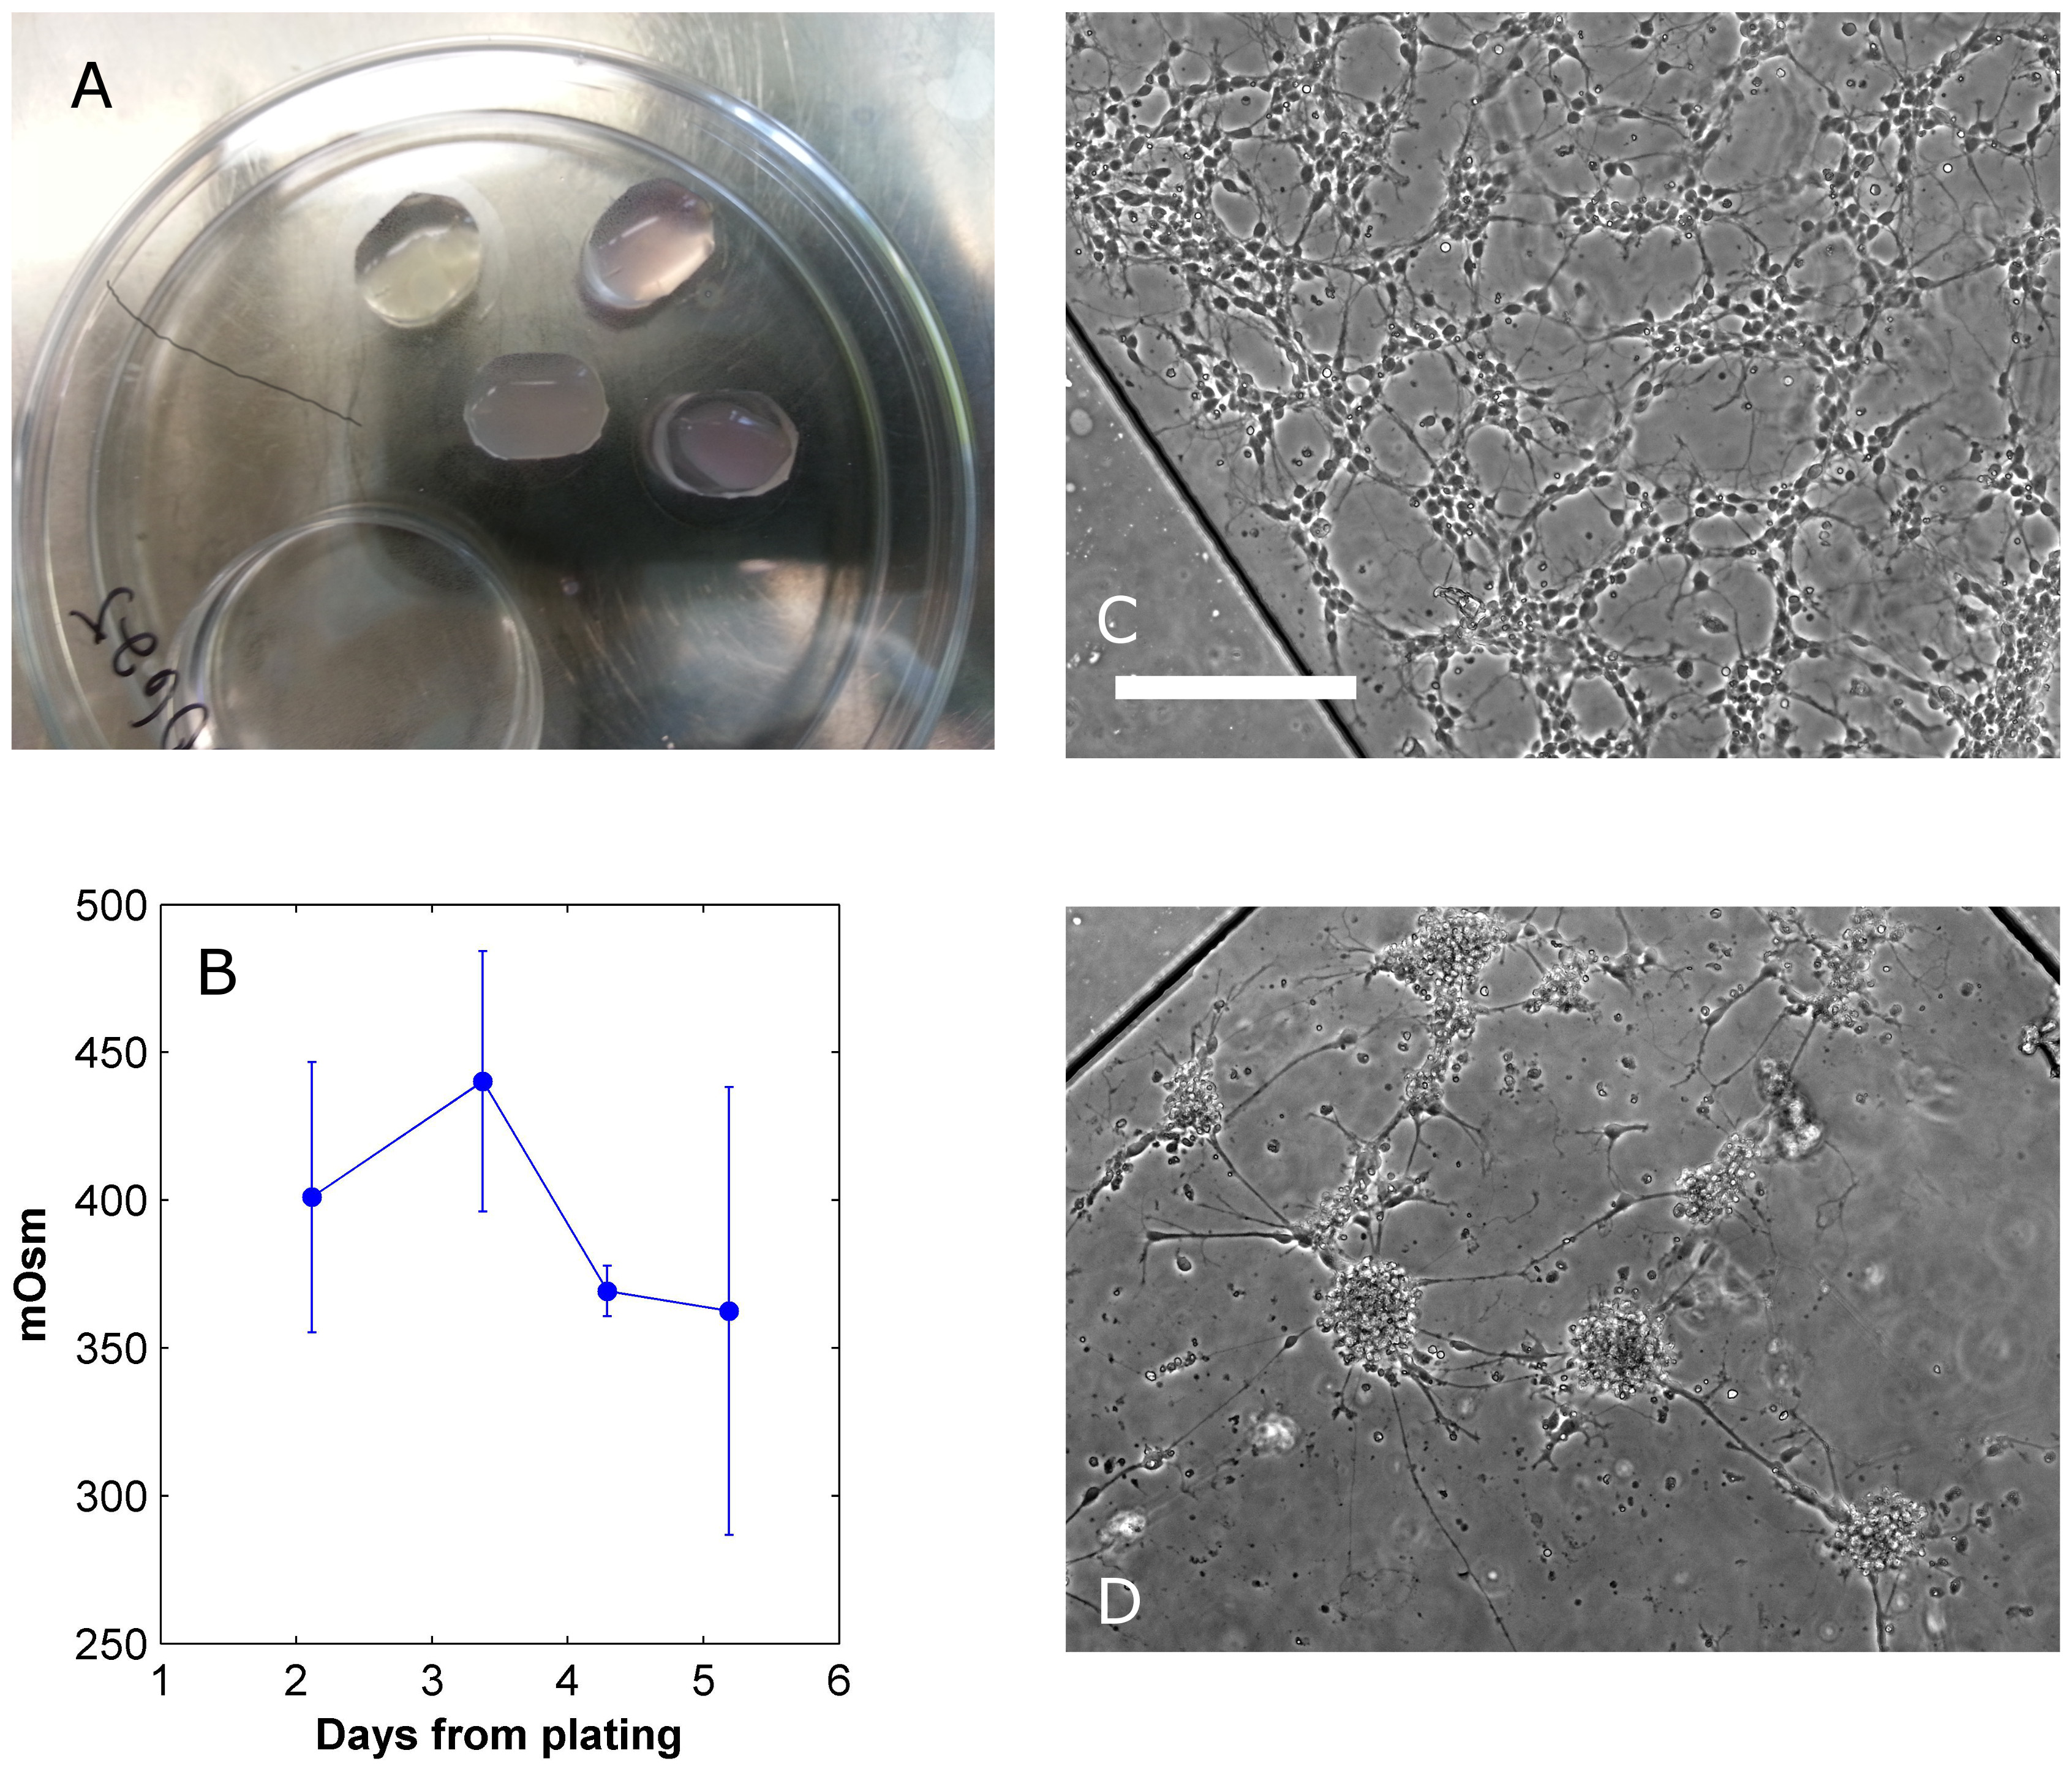
\includegraphics[width=14.3cm]{chapter4/figures/osmIssue/osmIssue.jpg}
            \caption[Effects of osmolarity drift in early protocol for long term culturing of neurons in microfluidic devices]{\textbf{The `drop on top' configuration results in excessive osmotic drifts and degeneration of the cultures.} (A) Top view of a group of devices illustrating the `drop on top' approach. (B) Osmolarity measurements taken from the drops on top of the devices in A during a maintenance protocol where the drop on top was changed every day. (C-D) Images of a culture growing in the `drop on top' configuration and where the drop was changed only twice weekly. Images are at 2 and 5 days \textit{in vitro}, respectively. By 5 days \textit{in vitro} the cell have aggregated and the glass surface remained relatively free of neurites and tissue, indicating degeneration (compare to figure \ref{fig:devices:tapeCultures} A,C which shows healthy cultures at the same age). Scale bar is \(200 \mu m\) long and is consistent for both images C and D.}
            \label{fig:devices:osmIssue}
        \end{figure}

        We tried to circumvent the evaporation issue by changing the drop on top of the devices every day (as opposed to twice weekly) and assessed the effectiveness by following the osmolarity of 4 devices for several days following the plating. Figure \ref{fig:devices:osmIssue} B shows that the osmolarity in this case was stable but still very high (values of \(\approx 400mOsm\) where as the osmolarity of our Neurobasal growth media is \(225 mOsm\)). A better solution was provided by switching to a maintenance routine where the devices were fully immersed in \(2.5-3 mL\) of culture media for the duration of the culture development (figure \ref{fig:devices:immersion}). Full details of this routine are provided in section \ref{sec:methods:culture}. The volumes of media applied to each sample in this approach are comparable to what is used in standard cell culture samples so media could be changed just twice a week without incurring excessive osmotic drifts. After 3 weeks of culturing in this approach, media osmolarity never drifted by more than \(30 mOsm\). Beyond this, the initial patchiness in adhesion led us to suspect that 30 minutes of PLL incubation, which is adequate for standard open surfaces, might be be insufficient in the case of microfluidic devices where the extreme surface to volume ratio might cause an increased flux of PLL molecules into the PDMS and reduce the effective concentration available for the glass surface. Consequently, we also modified the protocol to an overnight PLL incubation. With this modified protocol we were able to sustain neuronal cultures for long term (figure \ref{fig:devices:volDensIssue}) but still not ideally, as will be described in the next section.

        \begin{figure}[h]
           \centering
            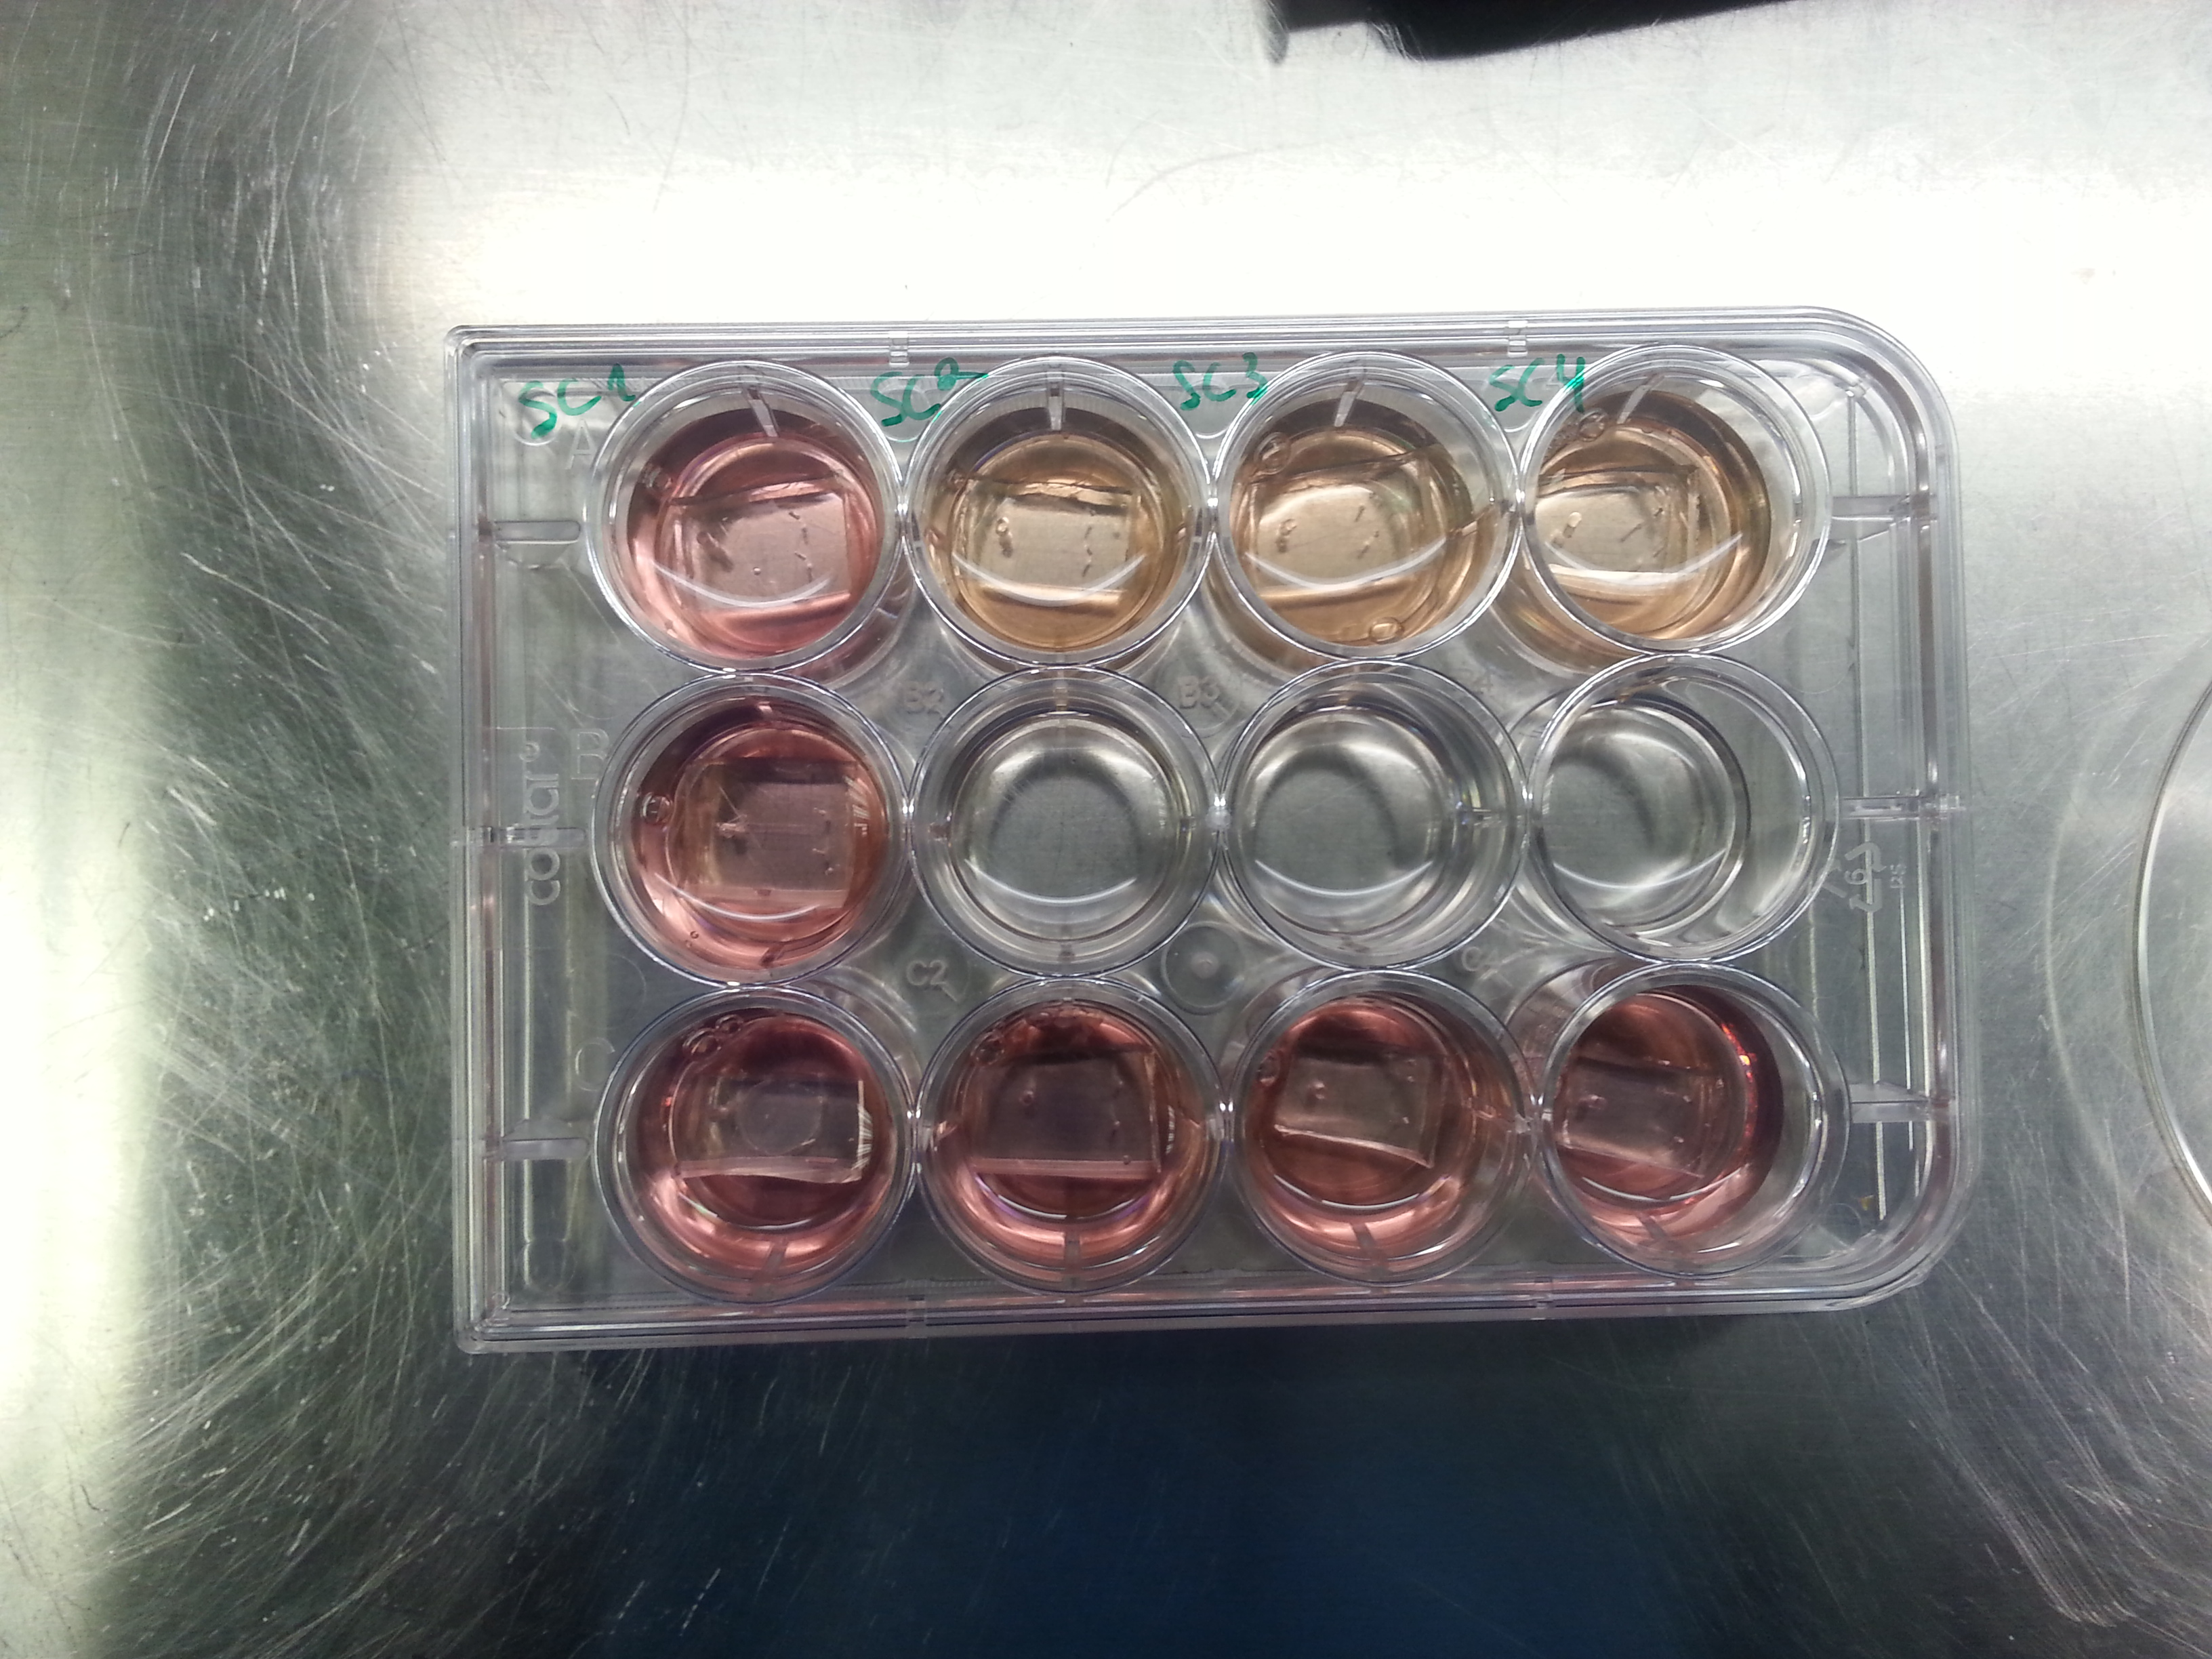
\includegraphics[width=12cm]{chapter4/figures/immersionMethod/12WellImmersion.jpg}
            \caption[The immersion maintenance configuration]{\textbf{The immersion configuration.} In this configuration, the devices were immersed in 12-wells with \(2.5-3 ml\) media each to prevent excessive osmotic drifts. This configuration required immersion 24 hours prior to seeding to release air trapped in the PDMS.}
            \label{fig:devices:immersion}
        \end{figure}


        \subsubsection{Considerations of factor circulation}
        \label{sec:devices:circulation}
        \begin{figure}[h]
           \centering
            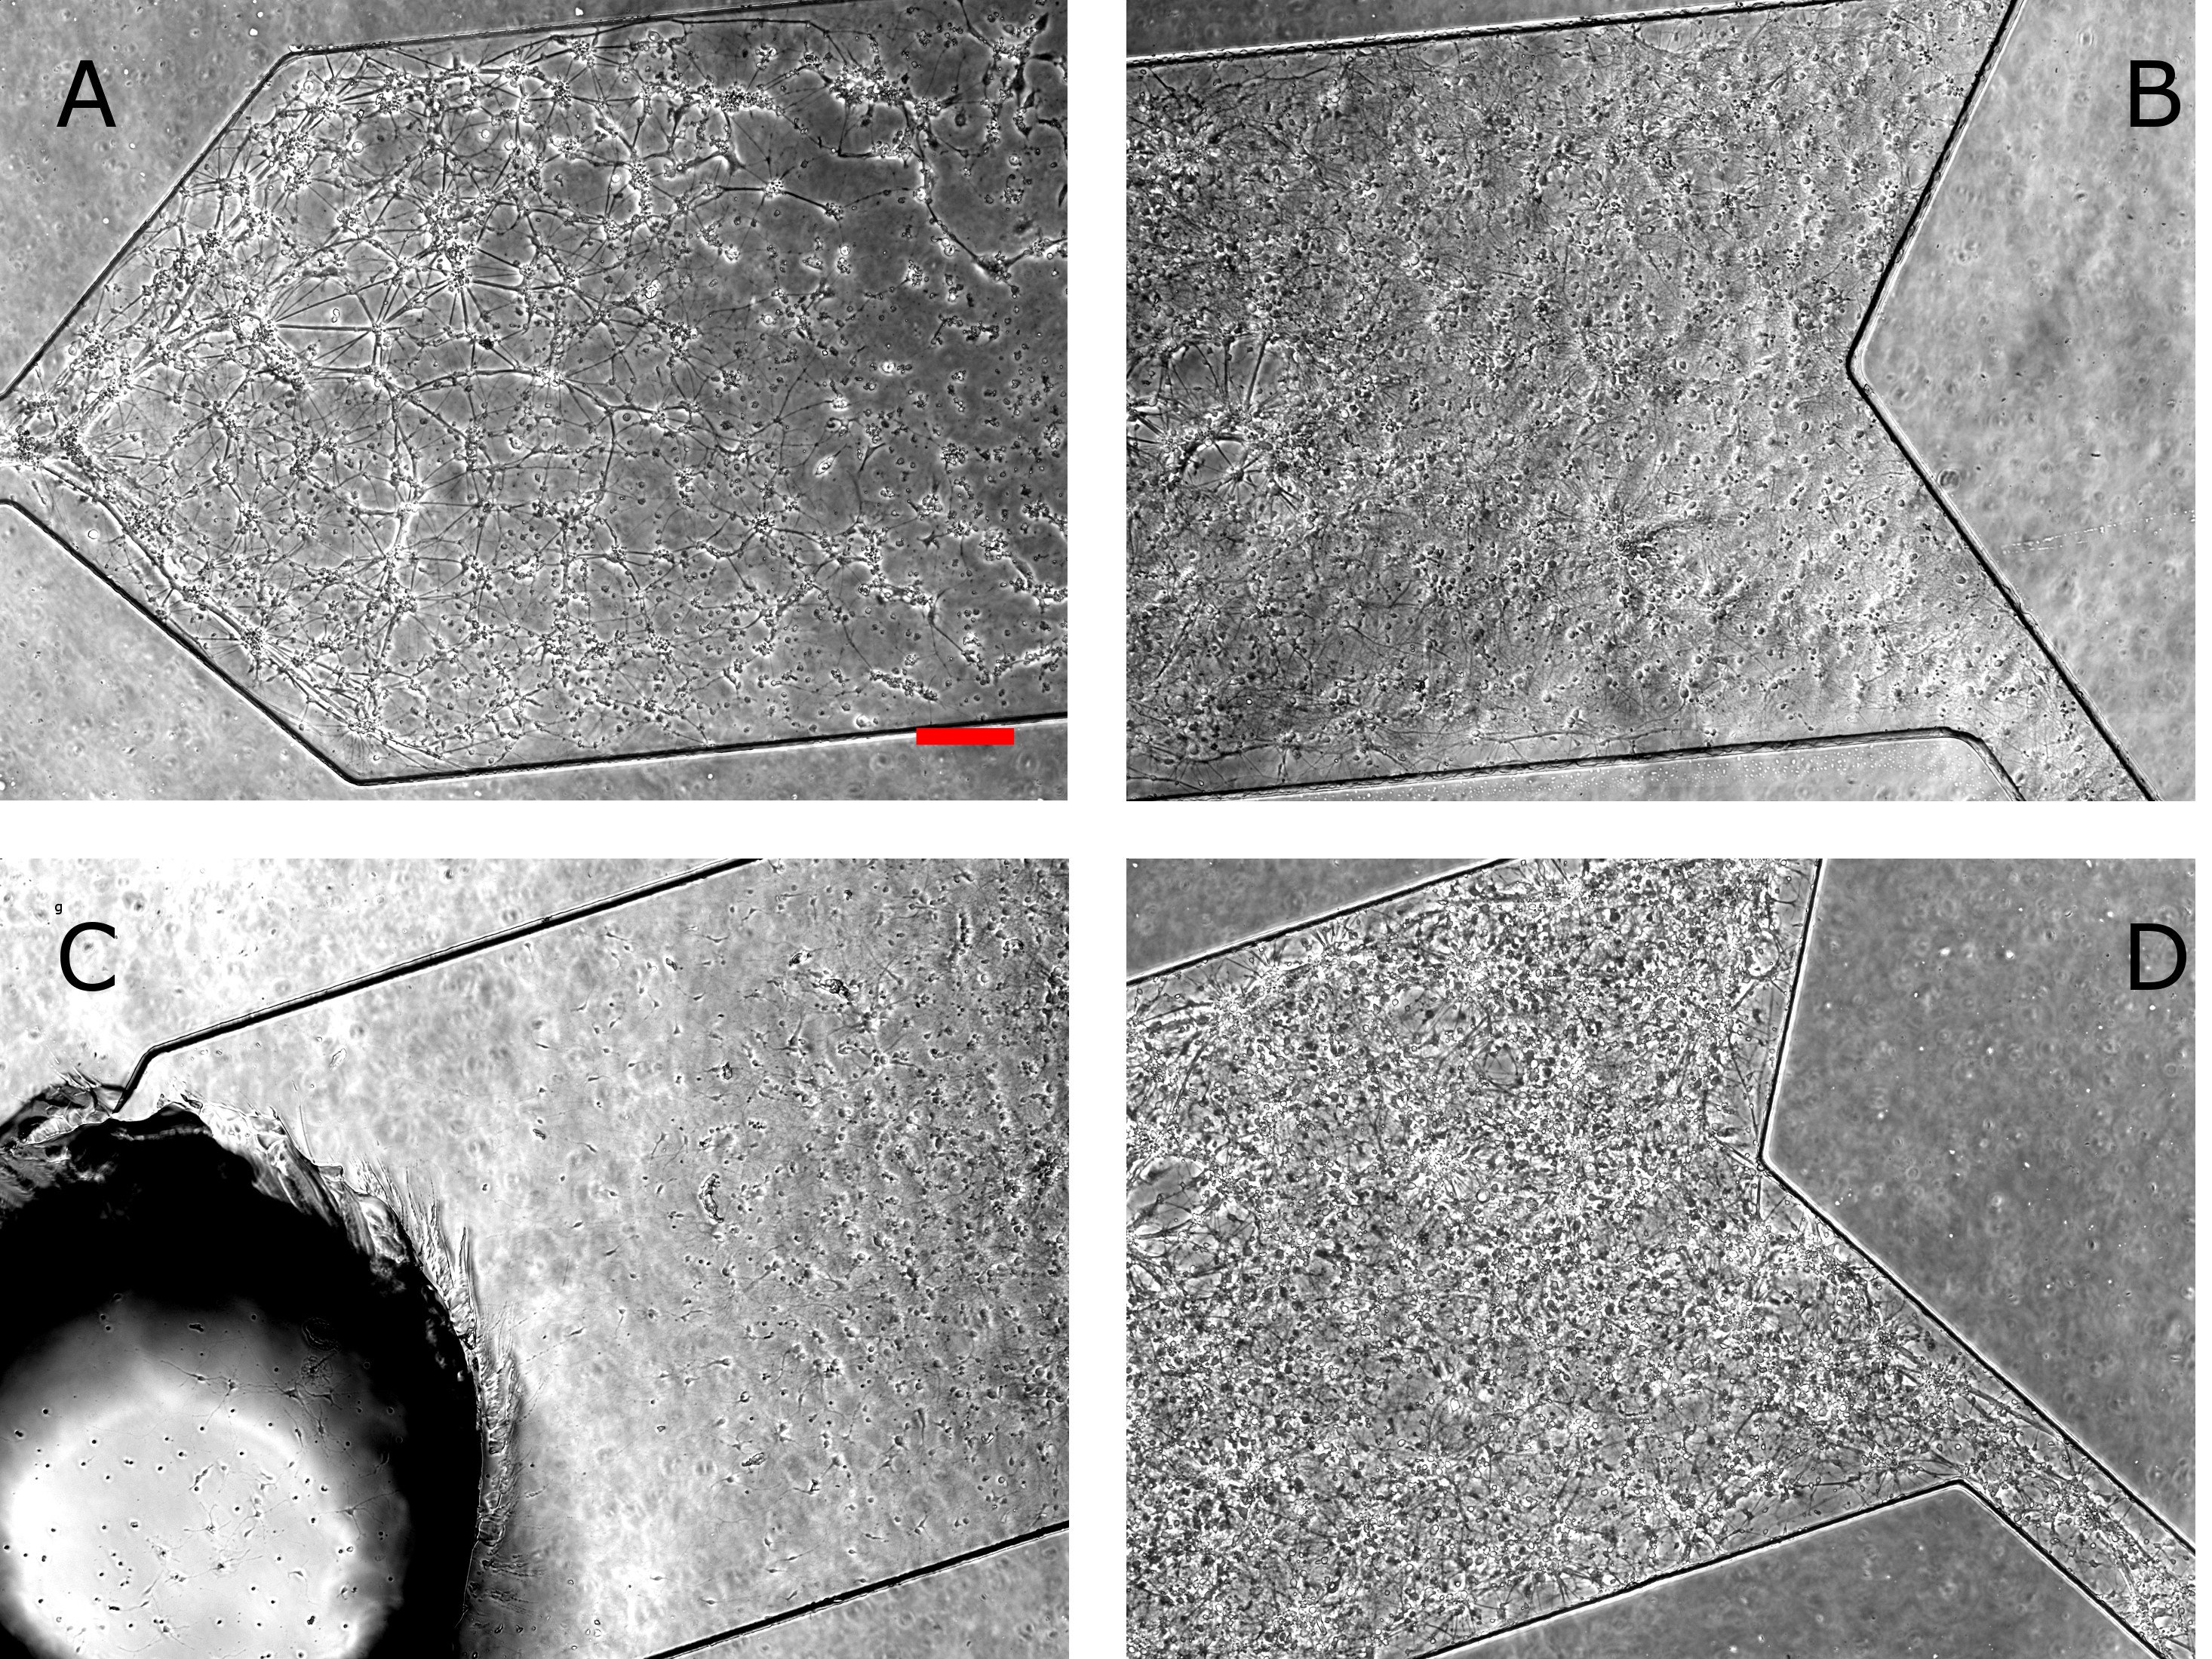
\includegraphics[width=12.4cm]{chapter4/figures/volDensIssue/volDensIssue.jpg}
            \caption[Demonstration of the limitations of circulation in planar microfluidic devices]{\textbf{A circulation bottleneck can emerge in microfluidic devices.} (A-B) Images of a culture growing in 3-port microfluidic devices where all the ports are \(0.8 mm\) in diameter. The images show the culture condition in the seeding port side and in the other side, respectively. Culture in the vicinity of the seeding port has degenerated, as indicated by the aggregation, prevalence of dead cells (observed as dots smaller then viable somata) and by the glass between the cells has remaining bare. (C-D) Images of a culture growing in 3-port microfluidic devices where one of the ports is twice as big (\(1.5 mm\)). Images show culture condition in both sides of the device as before. Images were taken at 12 days \textit{in vitro}. Seeding solution density was of \(40\times10^6 \frac{cells}{ml}\) which is equivalent to \(2600 \frac{cells}{mm^2}\) assuming homogenous distribution of the cells. Devices were maintained as described in section \ref{sec:methods:culture}. Scale bar is \(200 \mu m\) long and is consistent across all images.}
            \label{fig:devices:volDensIssue}
        \end{figure}
        Figure \ref{fig:devices:volDensIssue} A-B shows microscope images of two sides of an example device 12 days after seeding during which it was maintained using the modified protocol as described above. The part of the culture residing in the vicinity of the seeding port did not develop properly and was mostly degenerated. Remarkably, the part of the very same culture residing on the side opposite to the seeding port was able to develop properly and maintain a healthy appearance for several weeks. A hint as to the mechanism operating behind the above phenomena comes from devices where one of the ports was punched to be twice as big (figure \ref{fig:devices:volDensIssue} C-D). In this case the cells were seeded from one of the ports opposite to the large port. In these large port devices the whole culture developed healthily without any significant spatial differences. Another clue was provided by our exploration of devices with a larger architecture where the height of the channel was \(1 mm\) and its internal volume \(\approx 20 \mu L\). The density of the plating solution for these devices was calculated so that the plated area density would be as in the small devices, \(2600 \frac{cells}{mm^2}\). Nevertheless, culture grown in these larger devices never exhibited any sign of such spatially arranged degeneration and typically developed well for several weeks. We hypothesised that the most likely explanation for the above observations is that the configuration of small devices and small ports does not provide adequate circulation to remove metabolic by-products and provide fresh nutrients to all parts of the culture. The fact that the degeneration occurred in proximity to the seeding port could be explained either by the port being blocked by lumps of cells or by a existence of a gradient of cell density along the channel. In both cases there would be a large unmet circulatory demand around the seeding port. In the case of the large port or the large devices, a stronger diffusive coupling between the culture and the external bulk media is enabled so in those cases circulation was not an issue. Since the configuration of small devices and small ports was required to properly interface with the flow tubing and to reach the required flow speeds we experimented with reduced plating densities in hope that these will have reduced circulatory demands. Indeed we found that by decreasing the plating density 6 fold (giving an area density of \(\approx 450 \frac{cells}{mm^2}\)) the spatially arranged degeneration phenomenon disappeared.

        The observations described in this section demonstrate how microfluidic technology can impose conditions that are not normally met in standard preparations. The area density of \(2600 \frac{cell}{mm^2}\) seeded in the earlier versions of the protocol is high but still commonly used for many applications involving neuronal culture. In those cases the culture is in immediate contact with a large volume of bulk media which readily supplies nutrients and removes by-products via diffusion. In our microfluidic devices, the internal volume of media is 3 orders of magnitude reduced (\(\approx 1 \mu L\)) and it is only in this extreme configuration that circulation becomes an issue. This situation is similar to cases where non-vascularized 3D cultures develop a necrotic core due to the lack of oxygen and nutrient penetration.

        \subsubsection{Alternative bonding methods}
        \label{sec:devices:bonding}
        Plasma bonding is a lengthy process that needs to be applied to each sample separately and therefore is not well suited for producing large quantities of devices. Additionally, it is not practical for more complex devices involving several layers as having to apply plasma bonding methodology to each layer separately makes the production of every single device very time consuming and error prone. Consequently, we experimented with alternative bonding approaches that have been recently suggested for assembly of microfluidic devices \cite{samel2007fabrication,nath2010rapid}. Complete protocols and illustrations are provided in section \ref{sec:methods:bonding}.

         \begin{figure}[h]
            \centering
            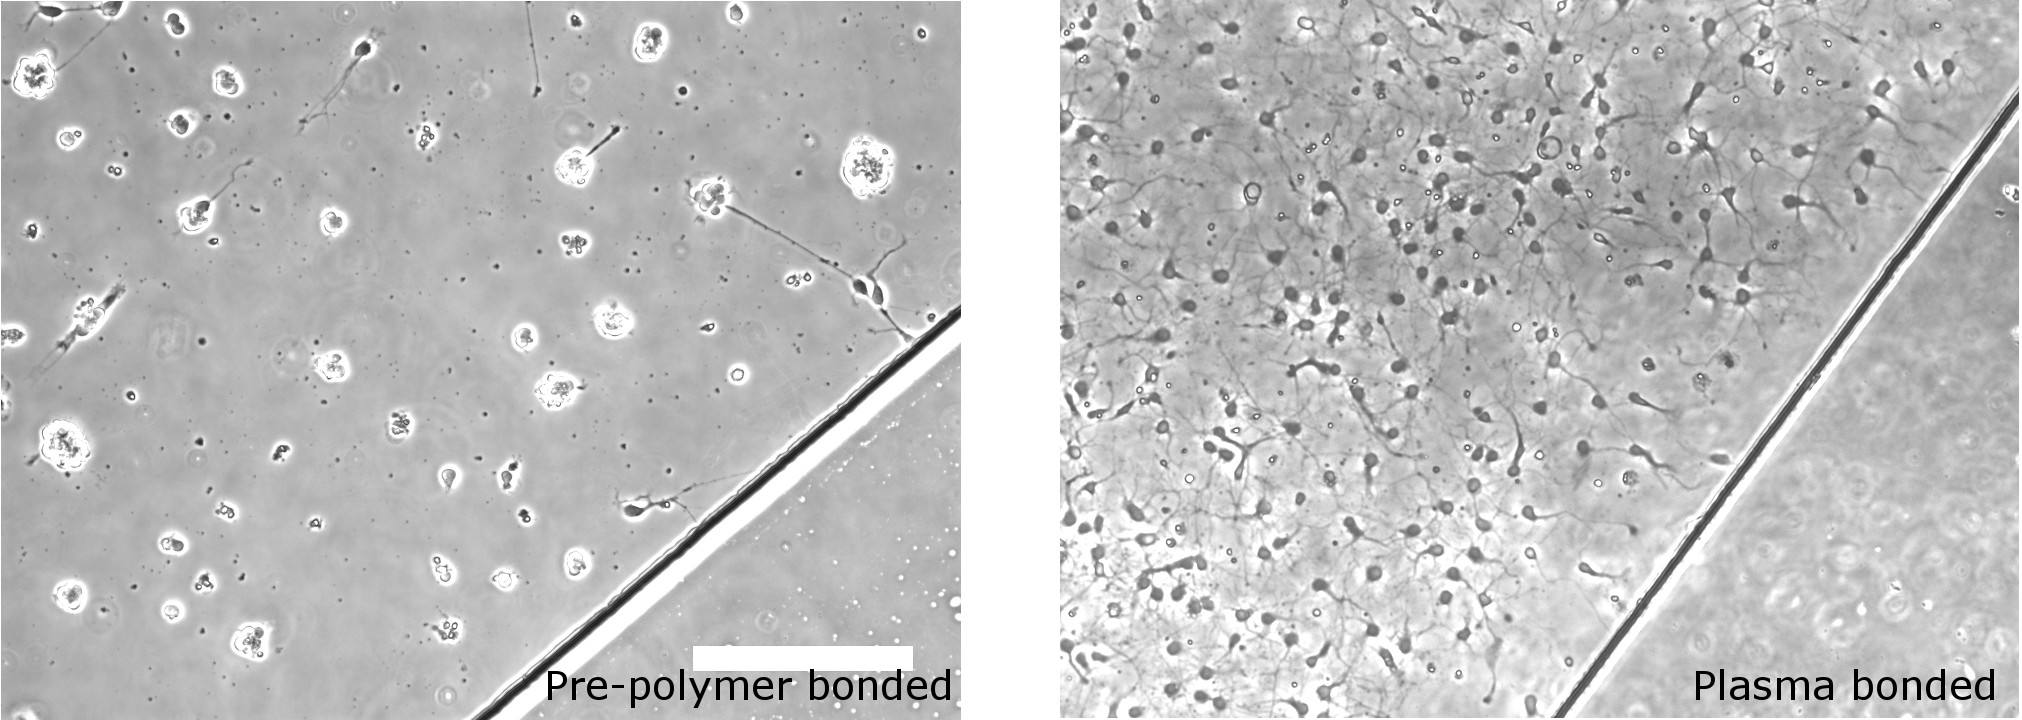
\includegraphics[width=15cm]{chapter4/figures/glueBonding/glueBondingComp.jpg}
            \caption[Effect of the pre-polymer bonding approach on the development of neuronal cultures in microfluidic devices]{\textbf{Contamination associated with pre-polymer bonding renders the surface unsuitable for neuronal adhesion.} Images comparing a culture growing in pre-polymer bonded devices to one growing in plasma bonded devices. The images were taken at 5 days \textit{in vitro}. Following bonding, the devices were subjected to identical surface preparation, seeding (density \(7\times10^6 \frac{cells}{ml}\)). and maintenance protocols (see sections \ref{sec:methods:surface} and \ref{sec:methods:culture}). Scale bar is \(200 \mu m\) long and is consistent across both images.}
            \label{fig:devices:glueBonding}
        \end{figure}


        The first approach attempted was to use the PDMS polymerization catalyst as an intermediate layer between the glass and PDMS bulk. The PDMS is dipped in catalyst solution, placed on top of the glass substrate and left to cure. This apparently induces further polymerization as well as partial covalent binding with the glass and results in a bond strength comparable or greater than plasma bonding \cite{samel2007fabrication}. We were able to achieve adequate bonding using this method but unfortunately the internal device surface proved to be completely inadequate for neuronal growth (figure \ref{fig:devices:glueBonding}. Interestingly, such a problem was not presented for other cell types such as astrocytes and HEK cells). This issue serves as another demonstration of the specific demands that are presented by neuronal culture. It is known that PDMS, when in contact with a surface, can contaminate the exposed areas around the point of contact through `leaching' of PDMS oligomers or curing agent molecules. Indeed it has been shown that PDMS sometime acts as a source of contamination interfering with neuronal growth inside microfluidic devices \cite{millet2007microfluidic}. The lack of adhesion reported here for the pre-polymer bound devices is probably an extreme manifestation of exactly these contamination processes.

        A different bonding alternative explored was that of using double sided silicone transfer tape \cite{nath2010rapid}. In this case channel features are not engraved into the PDMS through soft-lithography but simply cut out of the tape which is consequently joined with the glass surface. A square PDMS bulk with punched ports is joined to the top side of the tape to complete the body of the device. Since this method does not disrupt the surface coating of the non taped parts of the glass and can be performed in a sterile hood it opens the door for a new surface treatment approach. With tape based assembly the device can be taped to a pre-treated glass (surface-then-bond) whereas previously, with plasma bonding, the surface coating chemicals had to be introduced and incubated in the assembled device (bond-then-surface). This shift in paradigm allows to utilize the device geometry to control which parts of the treated surface will be exposed and available for culture adhesion and therefore offers an easy way of controlling its shape and size. This concept will be critical for the establishment of the microculture geometry in chapter \ref{chap:microculturePulses}.

        \begin{figure}[!htb]
            \centering
            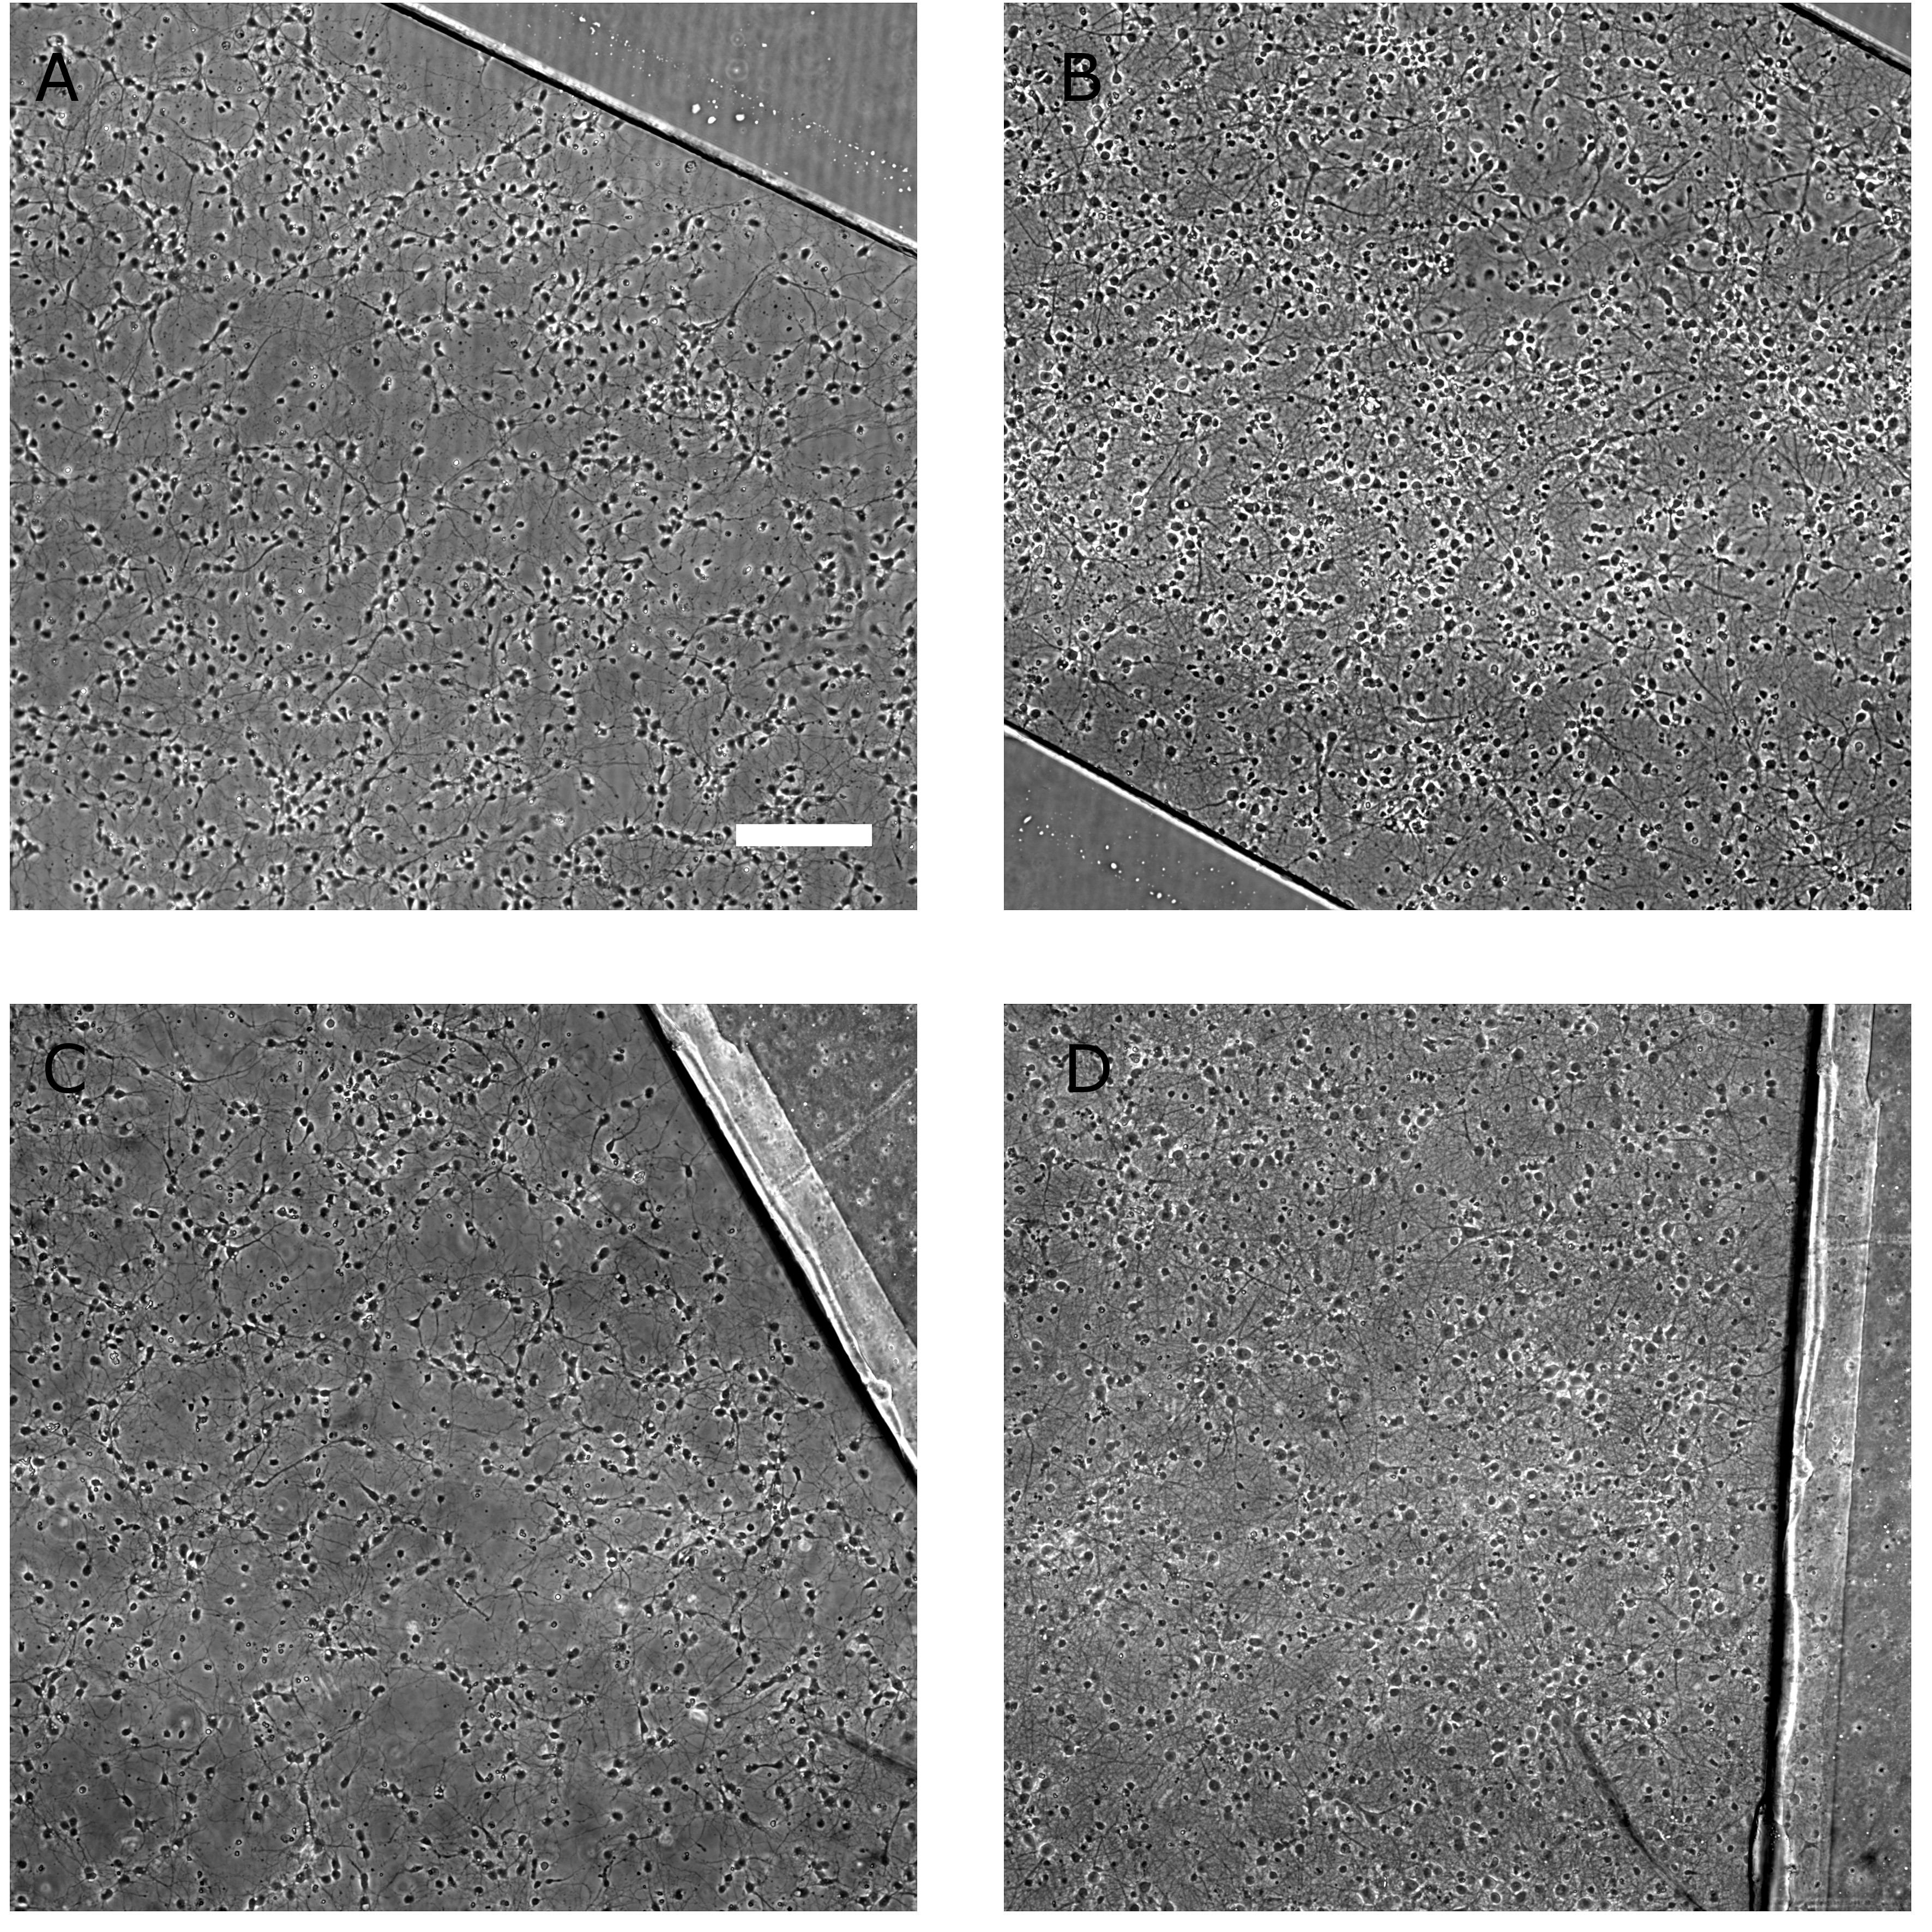
\includegraphics[width=15cm]{chapter4/figures/tapeCultures/tapeCultures.jpg}
            \caption[Comparison between cultures growing in plasma bonded devices and tape based devices]{\textbf{Tape based device architecture is fully compatible with neuronal culture.} (A-B) Cultures growing in plasma bonded devices at ages 5 and 12 days \textit{in vitro}, respectively. (C-D) Cultures growing in tape based devices at different stages of development as above. Plasma bonded devices were subjected to `bond-then-surface' surface preparation approach whereas tape based devices were subjected to `surface-then-bond' (see section \ref{sec:methods:surface}). Both devices were seeded and maintained as described in section \ref{sec:methods:culture}. Seeding density was \(7\times10^6 \frac{cells}{ml}\). Cultures in plasma bonded and tape devices are indistinguishable. Scale bar is \(200 \mu m\) long and is consistent across all images.}
            \label{fig:devices:tapeCultures}
        \end{figure}

        Figure \ref{fig:devices:tapeCultures} compares cultures grown in plasma bonded devices to ones grown in tape based and using the surface treatment paradigms appropriately as discussed above. The cultures are indistinguishable and appear to develop identically over the 12 days of inspection. This shows that the silicone tape is safe for use with neuronal culture and does not leach significant amount of toxins onto the surface or media. This tape based assembly approach will be cardinal for the multilayered devices described in chapters \ref{chap:activityAndFlow} and \ref{chap:microculturePulses}.


        \subsubsection{Extraction of PDMS}
        PDMS extraction is the last topic described with regards to the development of the basic protocol. As was apparent from the results of section \ref{sec:devices:bonding}, traces of curing agent or short oligomer chains can be harmful to neuronal cultures grown in the presence of PDMS. Indeed, even though the maintenance protocol achieved in section \ref{sec:devices:circulation} did generally sustain neuronal cultures for at a couple of weeks \textit{in vitro}, there were occasions where the cultures did not develop adequately. We reasoned that PDMS leaching might play a role in that inconsistency and therefore decided to try and employ a protocol for extraction of toxic species out of the cured devices. The protocol follows the suggestion from \cite{millet2007microfluidic} and is detailed in section \ref{sec:methods:fabrication}. Figure \ref{fig:devices:extraction} compares cultures grown in standard devices to those grown in extracted devices from the same plating and using the same maintenance protocol. In this plating, the cultures in standard devices seemed to fasciculate early on and completely degenerated by 12 days \textit{in vitro} (n=5). In the extracted devices (n=10) there was no sign of such degeneration. It should be noted that the extraction process involves immersing the devices in highly toxic solvents such as pentane and xylenes. When these are not properly oven-baked out of the devices a highly violent toxic effect is generated with the cells dying immediately upon seeding (figure \ref{fig:devices:extraction} C). Faulty development in non-extracted devices was not always observed and could be attributed to a specific PDMS mixing batch or to interactions with other factors. Nevertheless, to maximize the consistency of the preparations we added PDMS extraction to the standard protocol.

        \begin{figure}[!htb]
            \centering
            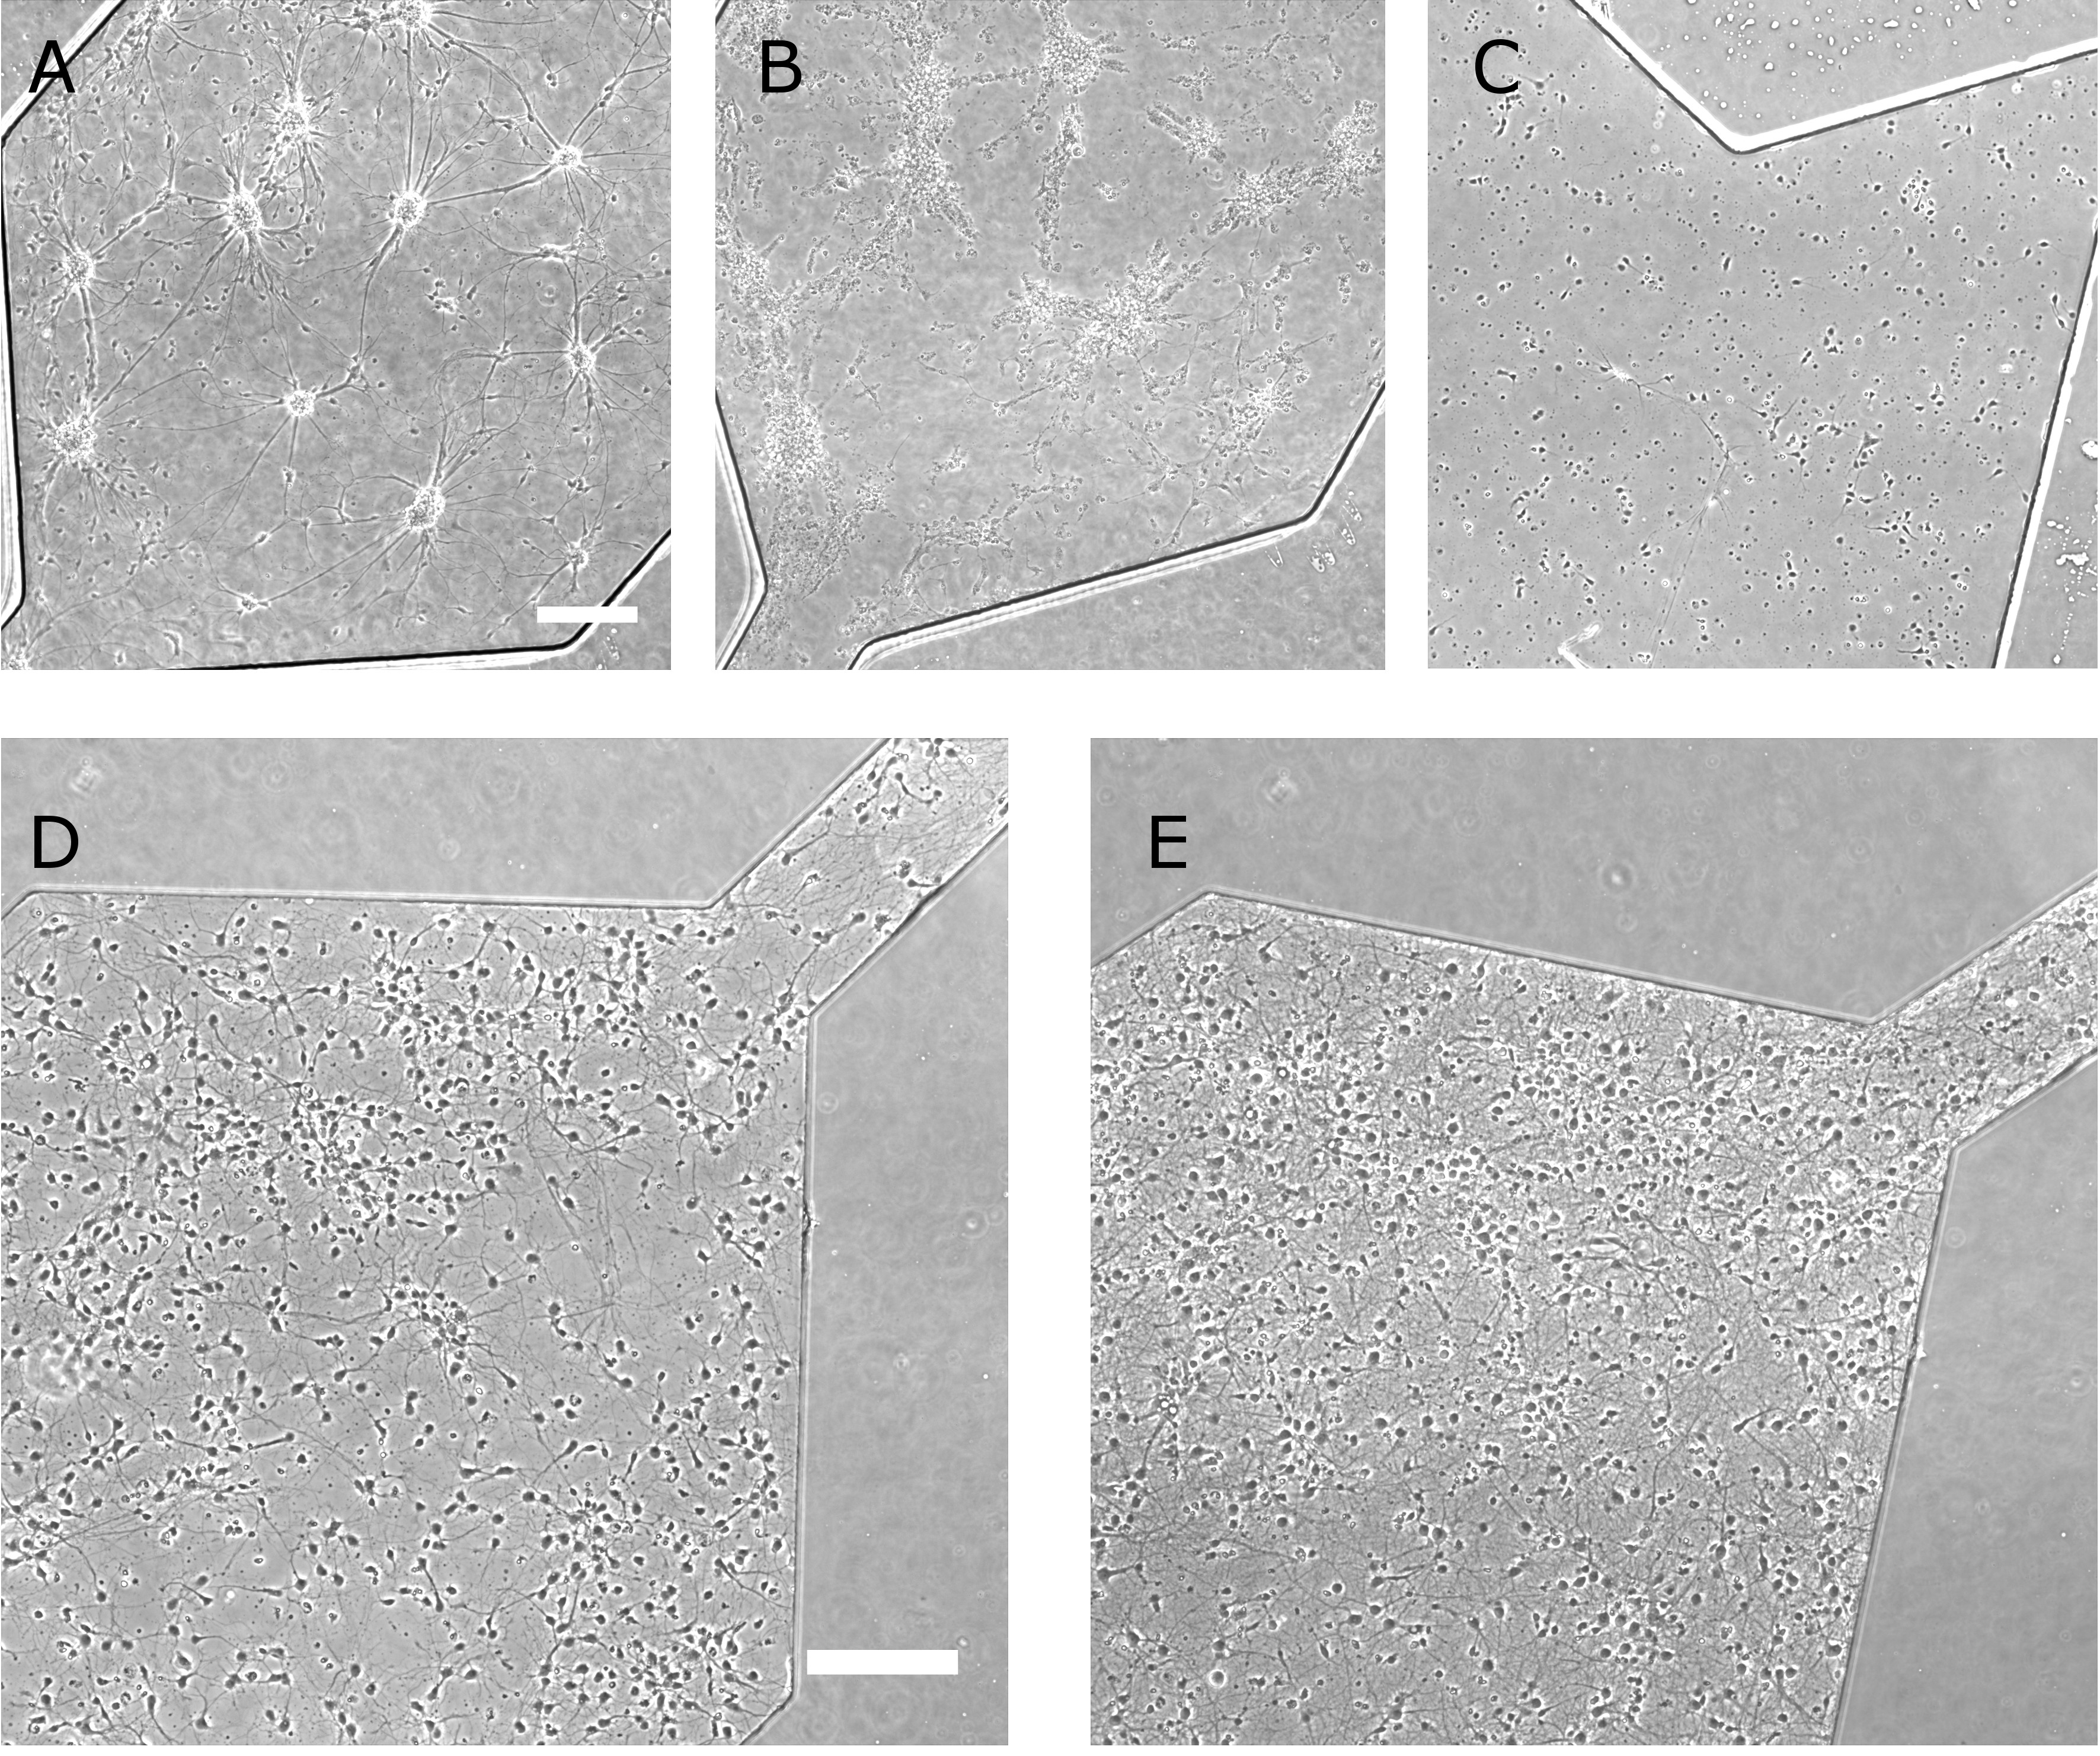
\includegraphics[width=15cm]{chapter4/figures/extraction/extractionIssue.jpg}
            \caption[Demonstration of PDMS related contaminations and the extraction procedure]{\textbf{Non extracted PDMS devices can leach out chemicals that are harmful to neuronal growth.} (A-B) Neuronal culture exhibiting adhesion and development issues that are thought to arise from PDMS leaching. Same culture is shown at ages 5 and 12 days \textit{in vitro}, respectively. (C) Culture seeded in a device made from extracted PDMS which was not baked long enough for removal of noxious extraction chemicals. Image was taken at 2 days \textit{in vitro}. (D-E) Cultures grown in extracted PDMS devices at 5 and 12 days \textit{in vitro}, respectively. These images represent the typical cultures achieved for the final protocol incorporating all the principles discussed in this section. All devices were plasma bonded (section \ref{sec:methods:fabrication}), subjected to `bond-then-surface' surface preparation (section \ref{sec:methods:surface}), seeded at a density of \(7\times10^6 \frac{cells}{ml}\) and maintained according to section \ref{sec:methods:culture}. Scale bar is \(200 \mu m\) long and is consistent across all images.}
            \label{fig:devices:extraction}
        \end{figure}

        To summarize, we have developed a protocol for long term growth of neuronal culture in planar (1-layer) microfluidic devices. We reviewed what we consider to be the important factors in the development of such protocols, namely, osmolarity, circulation of nutrients and oxygen, ease of assembly and leaching of chemicals from the construction materials (usually PDMS). Full details of the final protocol are provided in section \ref{sec:methods:culture}. This protocol is the basis for all the subsequent device types used in this Ph.D thesis. All of them will use the same preparation and maintenance routines and will differ only in the seeding density and volume which require adaptation to the specific device and culture geometry.

        \subsection{Growing microcultures in plasma bonded devices}
        \label{sec:devices:microcultures}

        As explained in section \ref{sec:devices:introduction}, controlling the physical extent of the culture is necessary in order to apply the interface shifting method in a way that produces physiologically relevant concentration pulses. Here we describe confinement of the cultures into microwells of a desired size. To add microwells to our device geometry, we produced a PDMS sheet with rectangular holes via thin film spinning on a silicon/SU-8 mold comprising pillars in the shape of the required microwells (see section \ref{sec:methods:fabrication}). To assemble the devices, the PDMS sheet was placed on a glass coverslip forming a reversible hydrophobic bond. The PDMS bulk with the engraved channel (as in figure \ref{fig:devices:basicDimensions}) was then plasma bonded to the PDMS sheet while being manually aligned to position the microwell within the channel borders (figure \ref{fig:devices:lithoMWell}). The devices were seeded at density of \(20\times10^6 \frac{cells}{ml}\) and volume of \(2 \mu L\). The seeding filled the entire device volume with cells which settled arbitrarily on the exposed PDMS or inside the microwells. After the initial seeding the devices were inspected under the microscope to check if there is adequate inhabitation of the microwells and subjected to flushing and re-seeding as necessary. As shown in figure \ref{fig:methods:mwProfile}, an undesirable side effect of the way the PDMS sheet was manufactured is that the microwells are produces with an elevated ridge around them. The ridge caused a directing of the cells around the microwells rather than into them which was the main reason why flushing and re-seeding was necessary at times. After obtaining adequate microwell inhabitation, the devices were left in the incubator for 2-3 hours for initial adhesion of the cells, then media was pulled through with a \(1 ml\) syringe. This pulling had a differential effect on the cells depending on their location, i.e., most of the cells on the PDMS surface were ripped off and removed by the pulling whereas the cells in the wells tended to stay put as they were protected from the shear. In this way, isolated neuronal microcultures were generated and they were maintained as described in section \ref{sec:methods:culture}.


        \begin{figure}[h]
            \centering
            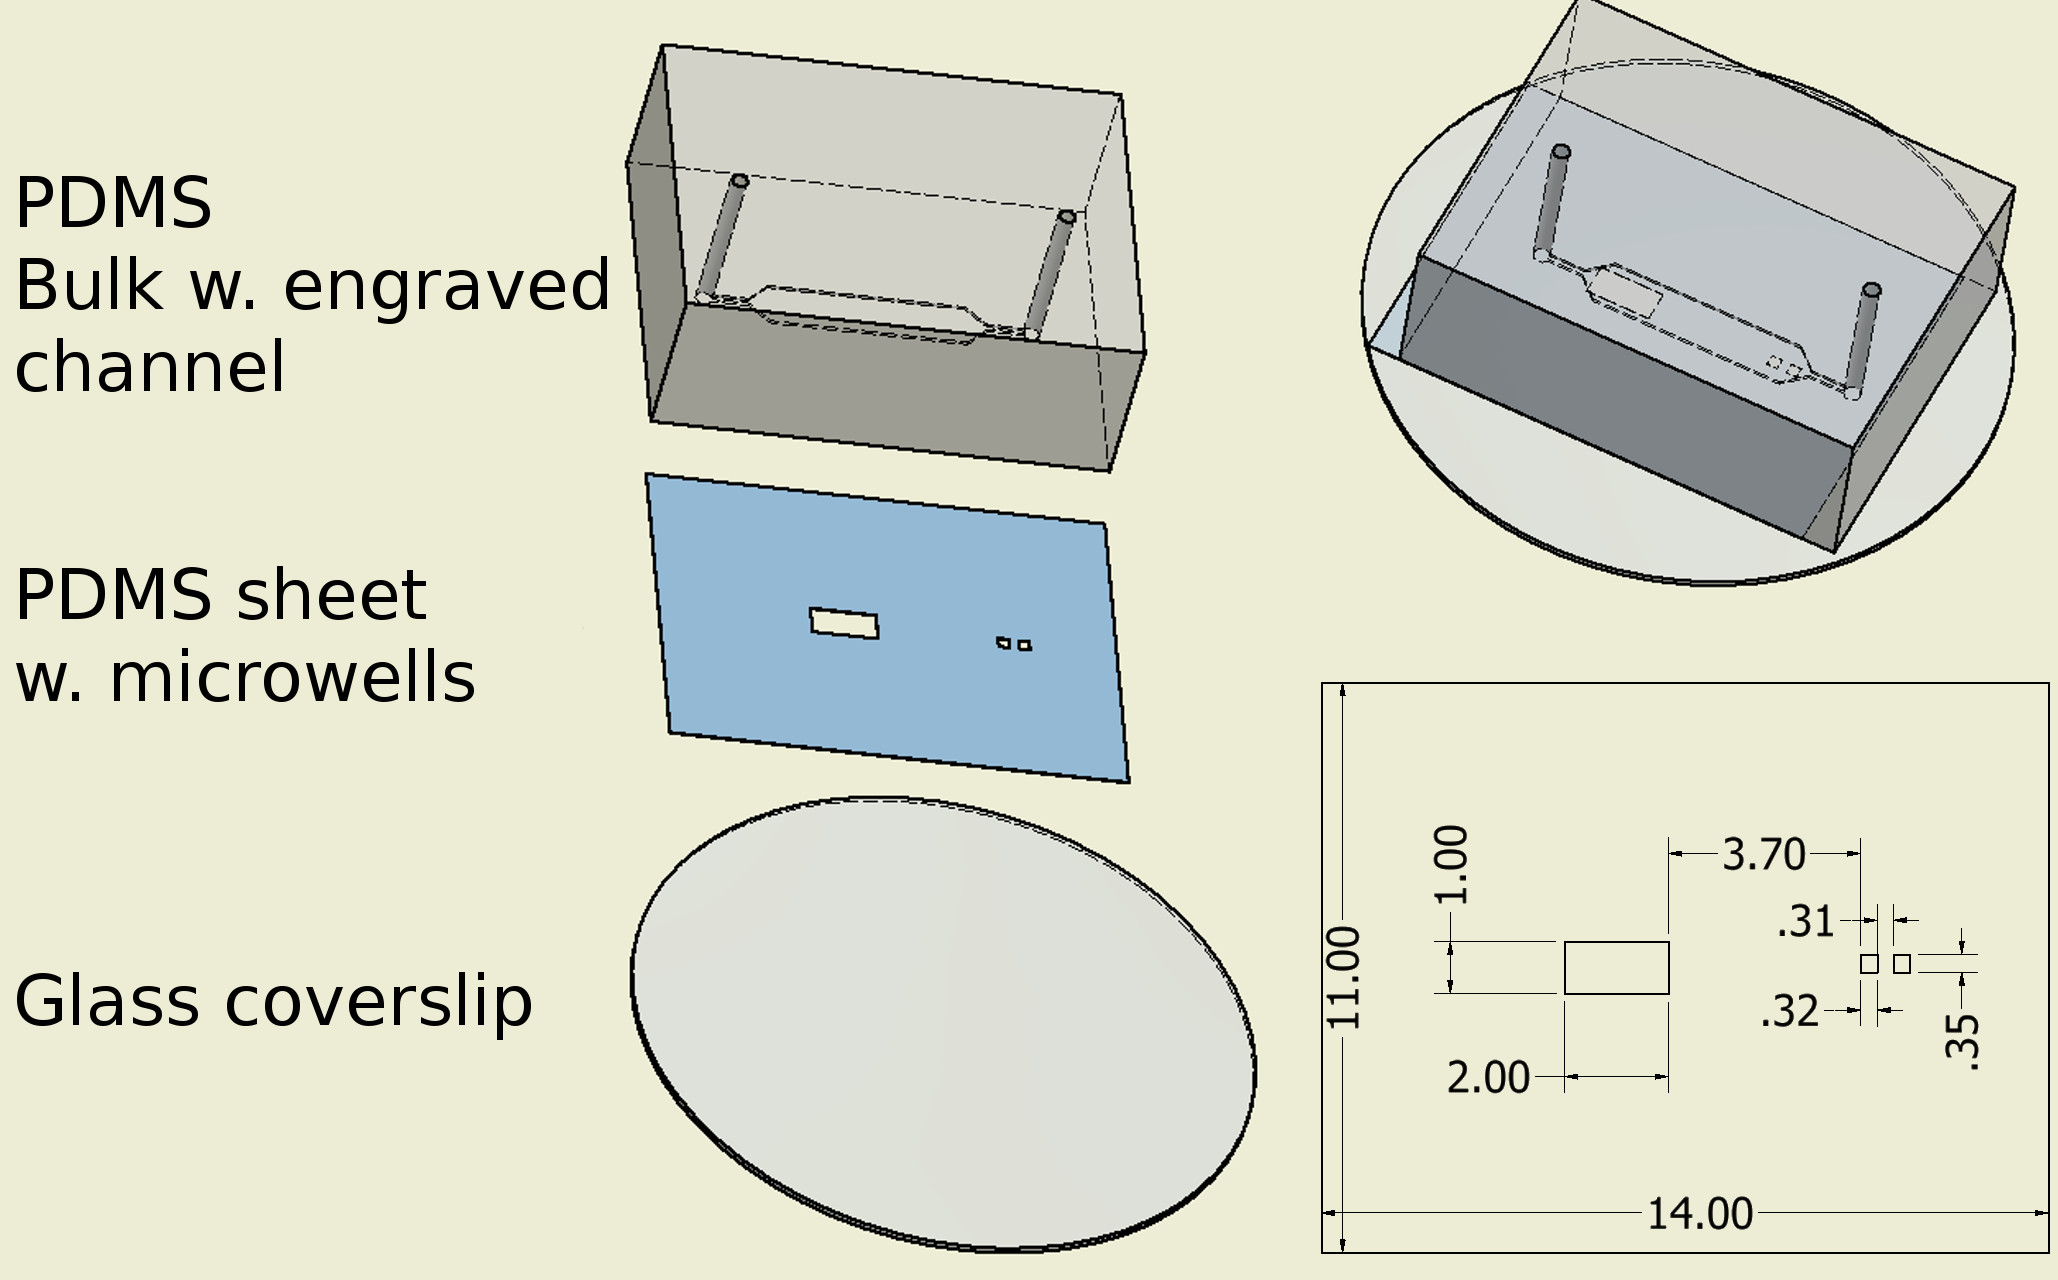
\includegraphics[width=7cm]{chapter4/figures/lithoMWell/lithoMWell.jpg}
            \caption[Schematics of the 2-layered microfluidic devices with microwells]{\textbf{Schematics of the 2-layered microfluidic devices with microwells.}
            The three components (PDMS bulk with an engraved microchannel, PDMS sheet and coverslip glass) of the device are shown separately and after bonding to illustrate how the the microwells are aligned to be within the channel boundaries. Dimensions of PDMS sheet are also presented in mm units. In this case, the microwells were of size \(350\times320 \mu m^2\). Dimensions of microchannel are as in figure \ref{fig:devices:basicDimensions}.}
            \label{fig:devices:lithoMWell}
        \end{figure}
        Section \ref{sec:devices:circulation} highlighted how, due to the small internal volume and narrow ports, our microfluidic devices can limit nutrient and oxygen circulation to the extent that necrosis is induced. In the case of the microcultures, however, the opposite extremity of factor circulation seemed to present itself. Initial attempts to grow microcultures under the aforementioned maintenance protocol resulted in the cells showing an initially good adhesion but failing to show any subsequent development and degenerating altogether by 5 days \textit{in vitro} (figure \ref{fig:devices:noSupport}). This degeneration was similar in time scales to the one caused by the osmotic drift but seemed to be more aggressive as the cells did very little even in the direction of initial sprouting of neurites. This type of degeneration is known to occur in small / low density cultures even in standard preparations (i.e., open surfaces, not microfluidic devices) \cite{kaech2006culturing} where it is presumed that the neurons are not able to generate a sufficient concentration of conditioning factors around them to sustain their development. The typical solution in this situation is to grow the cultures in proximity to a large pure astrocyte culture which shares the same media and secretes the required conditioning factors. This auxiliary astrocyte culture is sometime termed support culture. We followed this approach by adding two levels of support culture. One was harboured in a large well situated within the device several millimeters away from the microcultures (see figure \ref{fig:devices:lithoMWell}). A second one was a large culture plated outside the devices on the bare cover slip glass around the PDMS bulk. We found that the presence of these support cultures indeed prevented the aforementioned degeneration (figure \ref{fig:devices:mwDev}) and that both of them together were required for best results. We did not attempt growing pure astrocyte cultures for this as regular cortical cultures (which contain astrocytes) seemed sufficient to produce a beneficial effect.

        \begin{figure}[h]
            \centering
            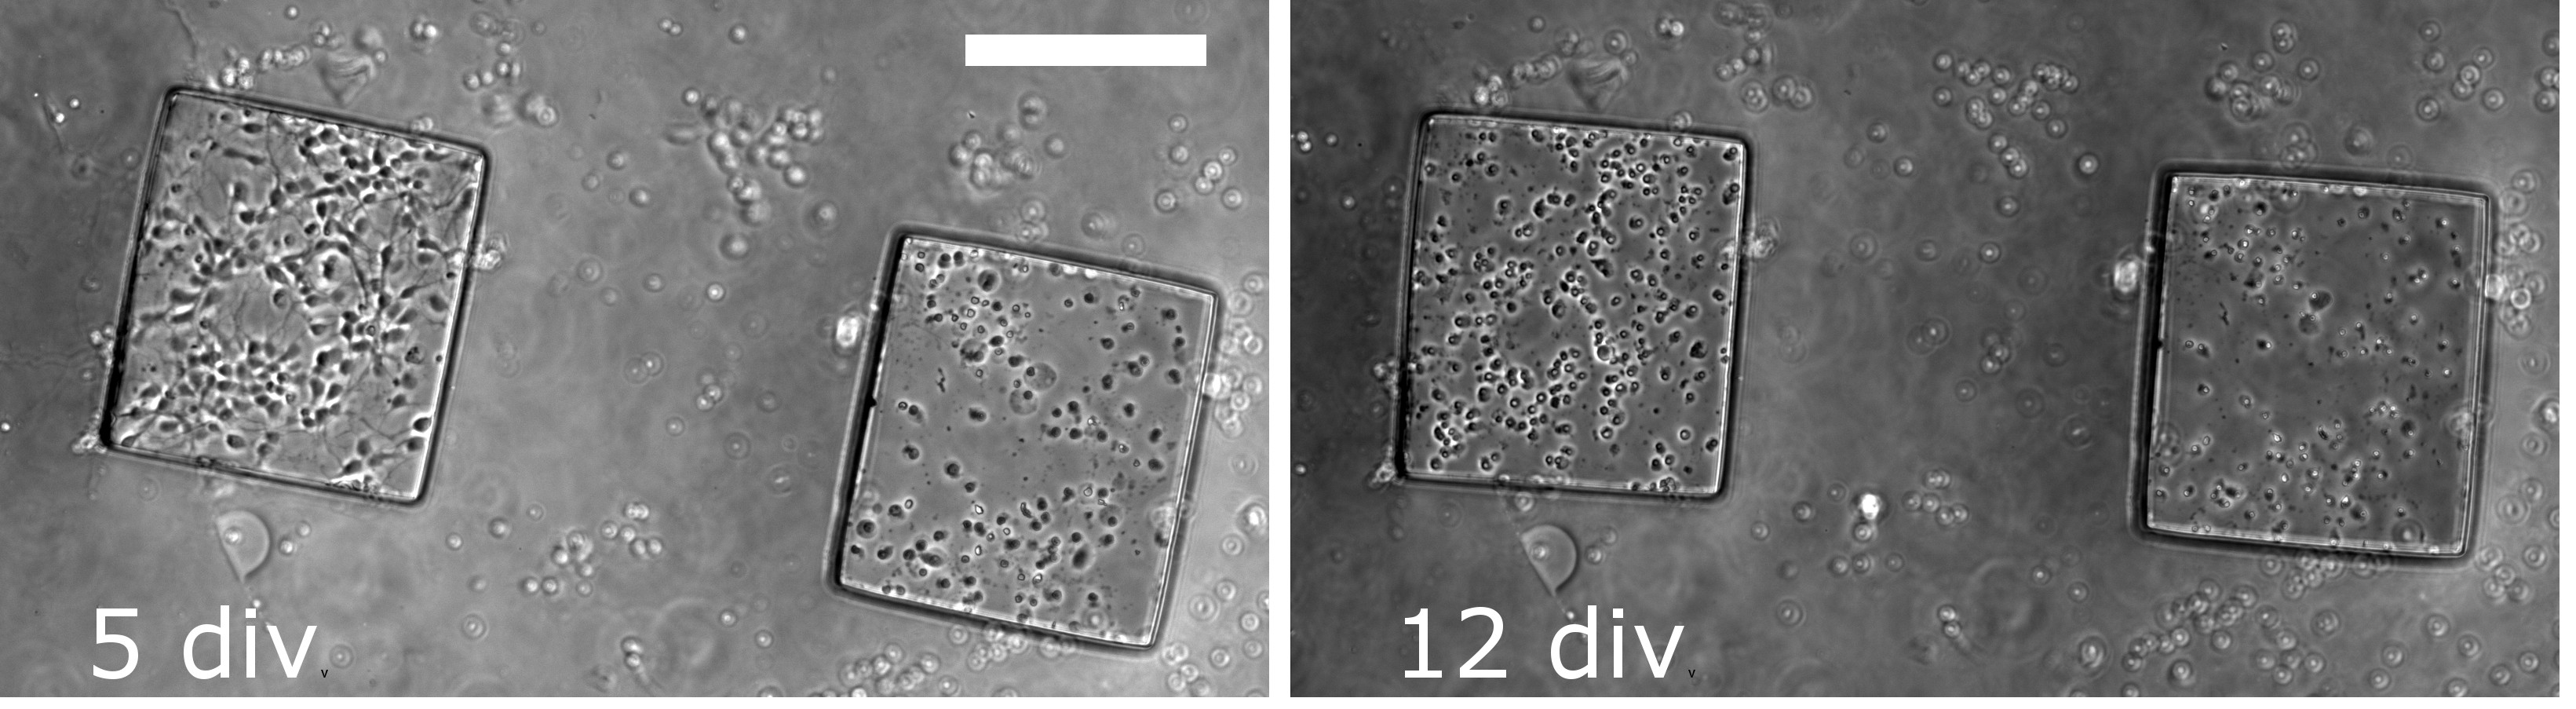
\includegraphics[width=13.8cm]{chapter4/figures/noSupport/noSupport.jpg}
            \caption[Neuronal microcultures growing without a support culture]{\textbf{Neuronal microcultures do not develop without a support culture.} Representative images of microcultures developing without seeding a support culture outside the device. The microwells were of size \(300\times270 \mu m^2\). Scale bar is \(200 \mu m\) long and is consistent across both images.}
            \label{fig:devices:noSupport}
        \end{figure}

        \begin{figure}[h]
            \centering
            \includegraphics[width=13.7cm]{chapter4/figures/microWellsDev/microwellsDev.jpg}
            \caption[Development of neuronal microcultures]{\textbf{Development of neuronal microcultures.} (A-B) Images of a neuronal microculture growing in a microwell of size \(400\times370 \mu m^2\) at 5 and 12 days \textit{in vitro}. (C-D) Images of two neuronal microcultures at developmental stages as above in microwells of size \(220\times190 \mu m^2\). Microcultures were seeded at a density of \(20\times10^6 \frac{cells}{ml}\), flushed and maintained as described in section \ref{sec:methods:culture}. Scale bar is \(200 \mu m\) long and is consistent across all images.}
            \label{fig:devices:mwDev}
        \end{figure}

        Since such microcultures are not a standard neuroscience model preparation and it is unknown what is the smallest size they can be made while still developing properly, we decided to conduct a quantitative examination of their viability. To that end, we designed devices with 3 different microwell sizes and followed their development over 12 days \textit{in vitro}. We counted the number of healthy cells in bright field images taken at 1, 5, 12 days \textit{in vitro} and calculated the proportion of cells dying between consecutive counting time points. This data are presented in figure \ref{fig:devices:mwStats} as a function of the density of cells in the well at the preceding time point and grouped by well size. This is compared to the same statistic computed in the same way for images of the standard cultures from section \ref{sec:devices:protocolDev} referred to here as macrocultures. It is evident from figure \ref{fig:devices:mwStats} A that, regardless of microwell size, the microculture death rates are strongly and negatively correlated with their density. This was corroborated with a linear regression analysis giving a statistically significant linear correlation (F-test, \(p=2\times10^{-4}\)). The macrocultures did not show such a density associated death rate (F-test, \(p=0.26\)) but the macroculture densities were much less variable so the analyzed density range was smaller. The averaged death rates of the macro- and microcultures are compared in figure \ref{fig:devices:mwStats} B. Microcultures of all 3 sizes exhibited a significantly higher death rate than the macrocultures (unbalanced t-test, \(p=2\times10^{-5}, 0.0012, 0.0027\) for well edge sizes \(200,300,400 \mu m\), respectively).

        Since microculture densities appeared to be a key factor in their long term viability we also performed a similar comparison with the microculture data restricted just to densities higher than \(1500\frac{cells}{mm^2}\). This density threshold was selected because the data beyond it did not show a density dependent trend which meant that the beneficial effects were saturated. Indeed the death rates at such high density microcultures were reduced and the large \(400 \mu m\) ones exhibited death rates indistinguishable from those in macrocultures (unbalanced t-test, p=0.23). Smaller high density microcultures of sizes \(200\) and \(300 \mu m\) still showed a significantly larger death rate (unbalanced t-test, p=0.0012 and 0.0012, respectively).

        The above data are consistent with the notion that neuronal cultures need to generate an environment of conditioning factors around the cells to support their own development. Since this environment comprises secreted factors its buildup would strongly depend on the density and the size of the culture. Indeed the effect of both of these parameters is evident in the data shown here and a practical heuristic emerges that microcultures larger then \(400\times400 \mu m^2\) and denser than \(1500 \frac{cell}{mm^2}\) have a potential of developing as well as macrocultures.

        \begin{figure}[h]
            \centering
            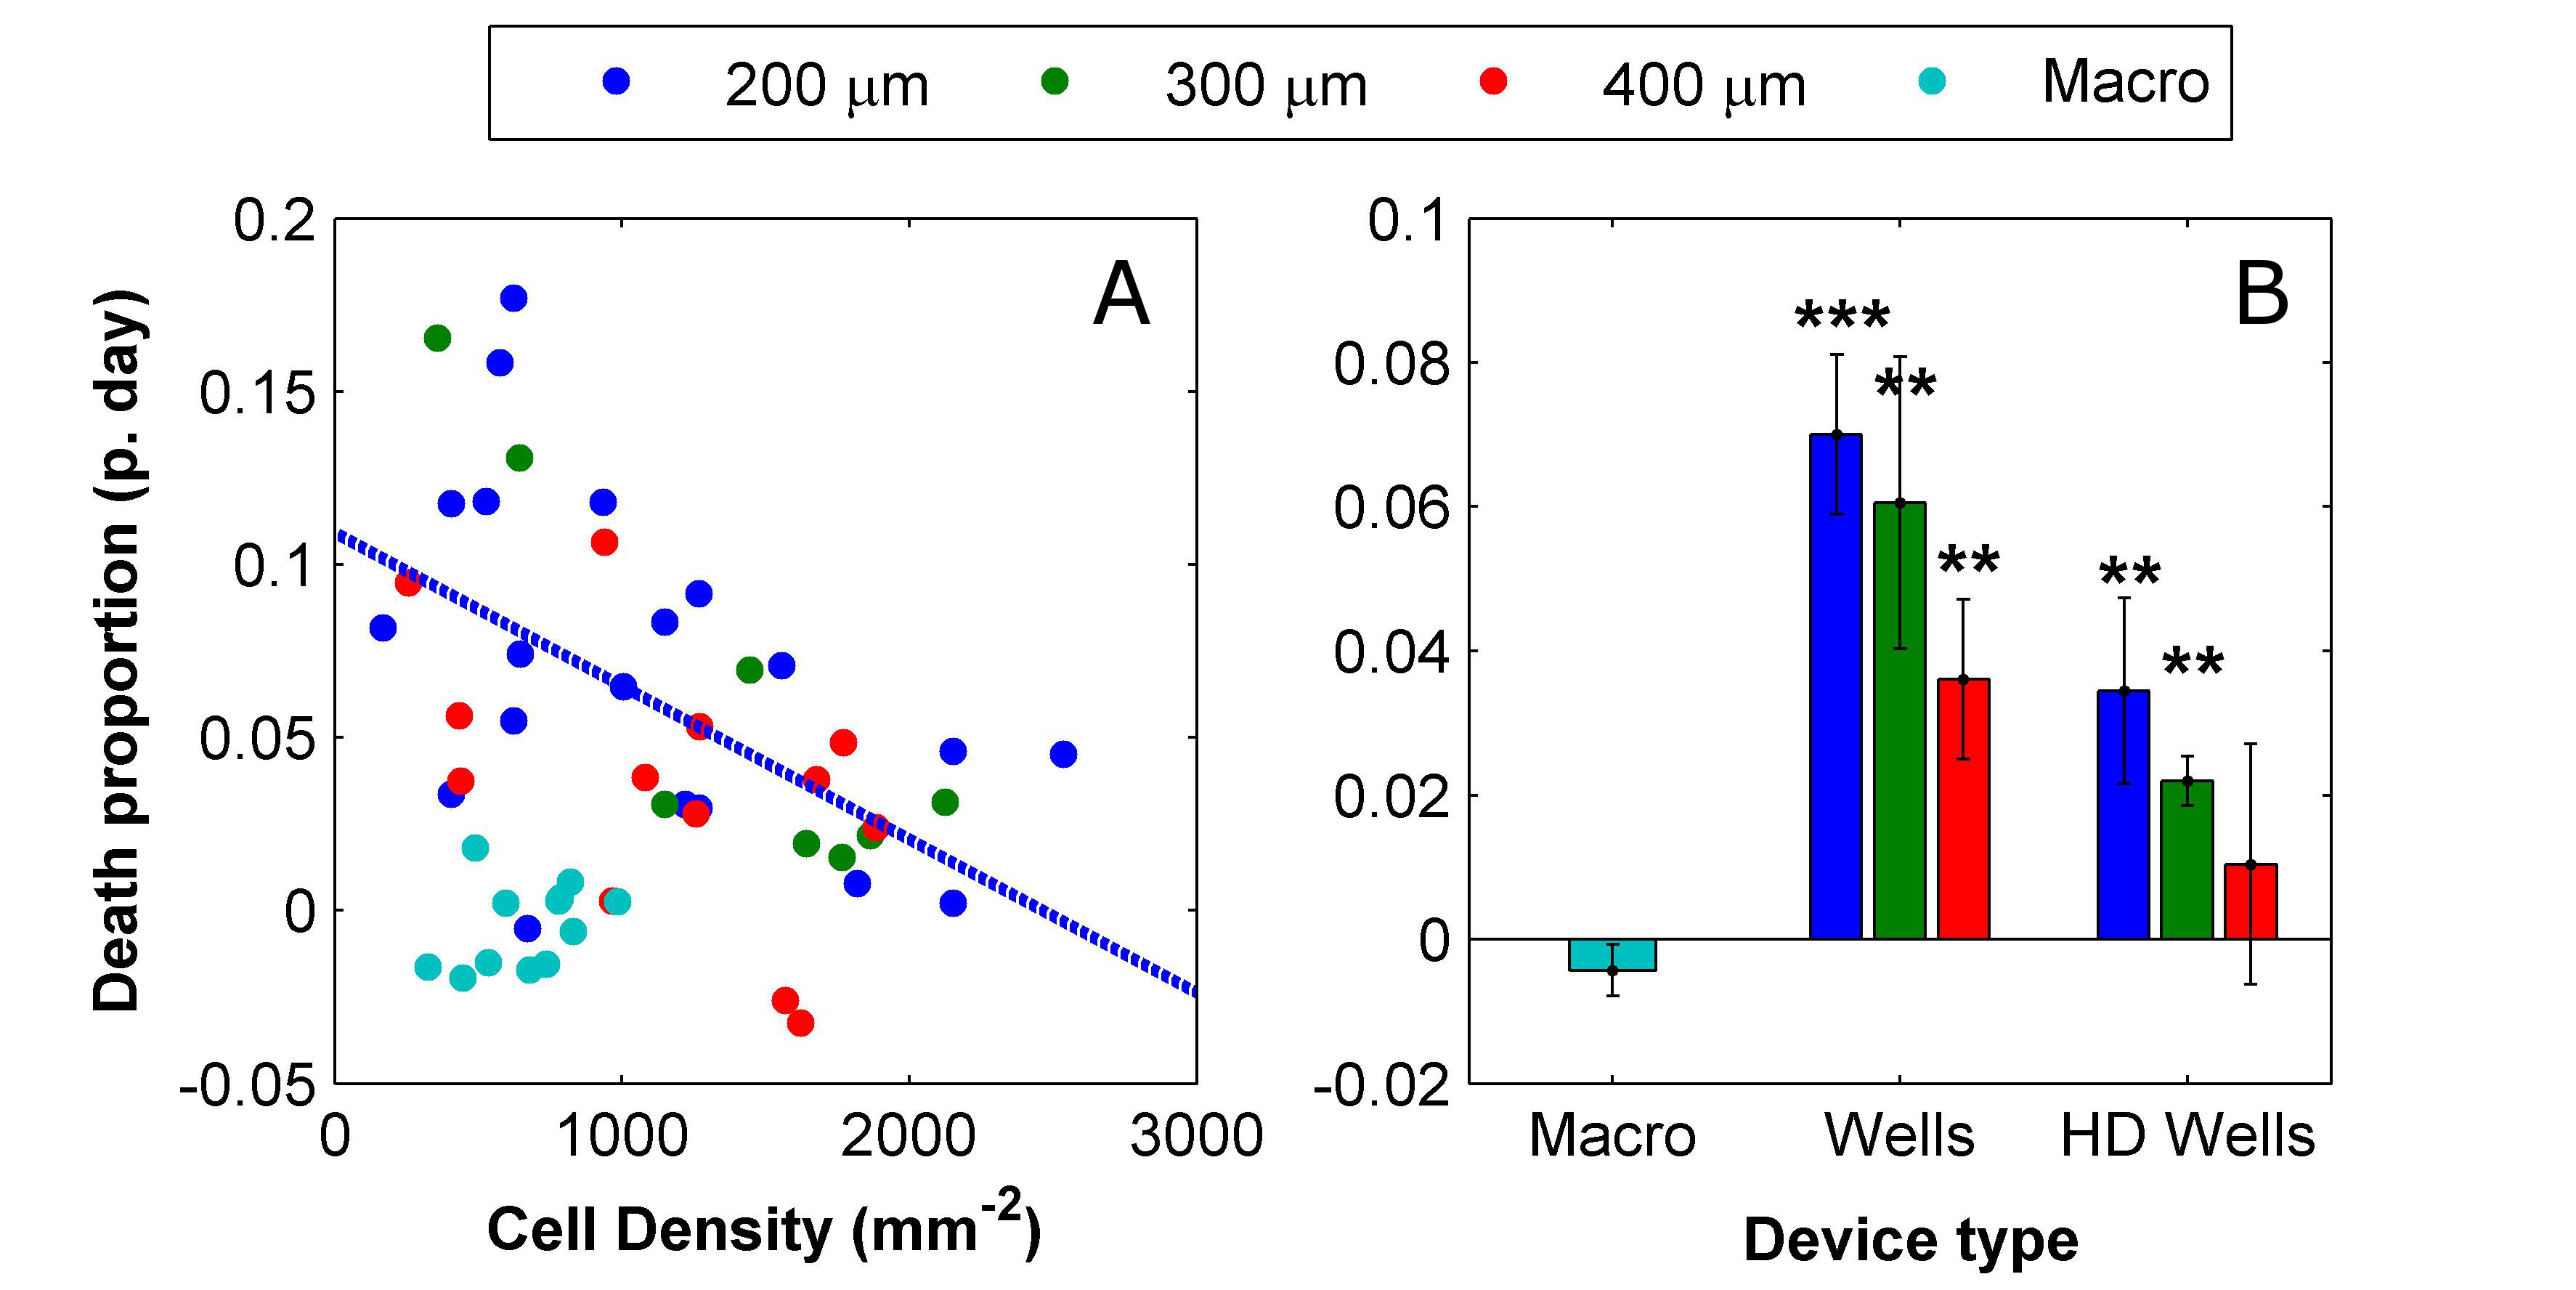
\includegraphics[width=15cm]{chapter4/figures/microWellsStats/mwStats.jpg}
            \caption[Statistics of microculture viability over development]{\textbf{The viability of the microcultures is correlated with their density and size.} (A) Scatter plot of the proportion of dead cells observed in the microcultures and macrocultures between consecutive counting time points as a function of microculture density. Each point represents a comparison between counts at 2 consecutive time points. Cells were counted at 1, 5 and 12 days \textit{in vitro}. Death proportion is normalized to the number of days between the counts. Data is color coded according to microwell size or if it is a macroculture. (B) Comparison of mean proportional death rates between all the microcultures or microcultures with density higher than \(1500 \frac{cells}{mm^2}\) and macrocultures. The data is based on 44 microcultures and 9 macrocultures from 4 different platings.}
            \label{fig:devices:mwStats}
        \end{figure}

        We would like to conclude this section by making a note about the quality of isolation of the microcultures. Since the devices considered here were assembled using plasma bonding, the surface treatment had to follow the `bind-then-surface' approach. This means that the assembled devices were filled and incubated with surface coating solution (PLL) so all exposed internal surfaces were actually chemically prepared for cell adhesion. This means that cells from within the wells were free to send neurites out onto the PDMS surface and even to migrate there. Additionally, the flushing procedure applied after the seeding was imperfect and sometimes left a substantial amount of cells on the PDMS sheet surface. This lack of restriction meant that after two weeks of growth the microcultures had significant innervation from neurons outside of the well (figure \ref{fig:devices:mwIso}). Axons seemed to traverse the entire distance between the the microwells and the large support well which was located \(3.7 mm\) away. This lack of isolation defeats the purpose for which the microwells were designed. This issue is solved in chapter \ref{chap:microculturePulses} where tape based design allows a `surface-then-bond' approach whereby only the well bottom is chemically prepared for cell adhesion.


        \begin{figure}[h]
            \centering
            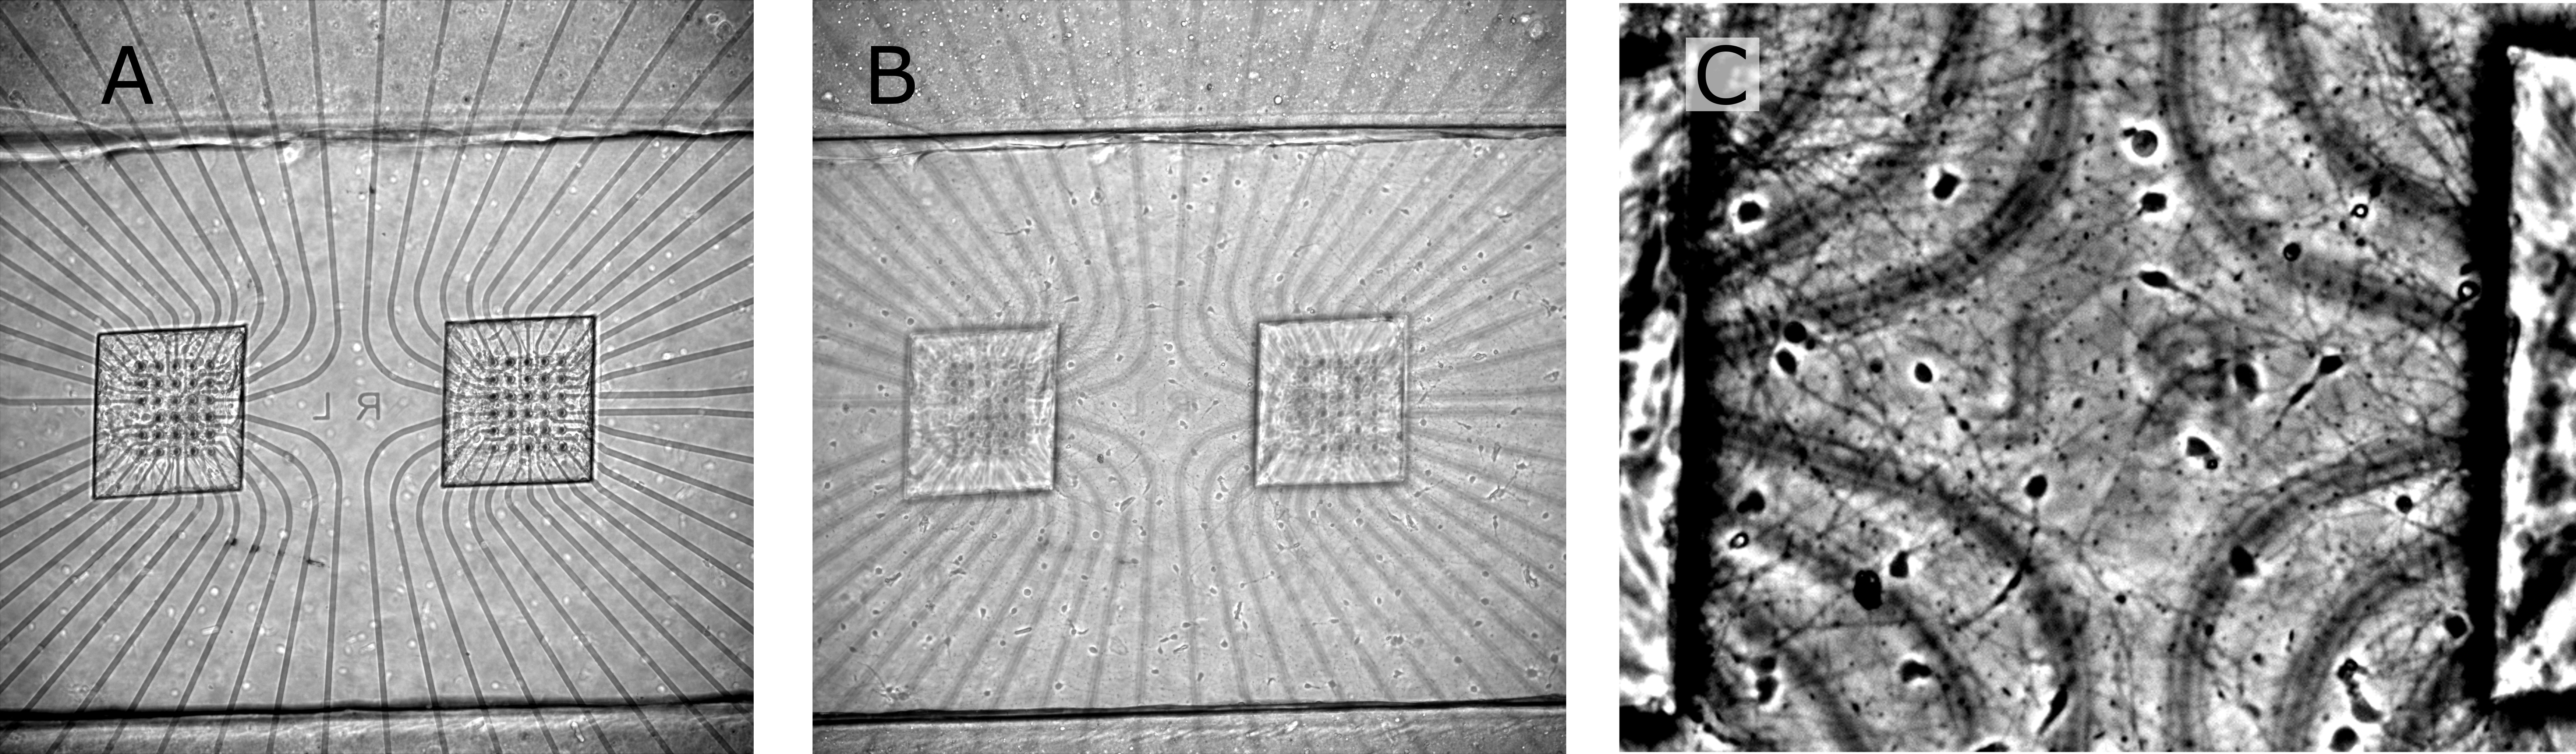
\includegraphics[width=15cm]{chapter4/figures/microWellsIsolation/isolationIssue.jpg}
            \caption[Demonstration of the microculture isolation issue with the bond-then-surface approach]{\textbf{Microcultures are not well restricted to the microwell area with bond-then-surface approach.} (A) Image of microcultures growing on top of commercial microelectrode arrays at 12 days \textit{in vitro}. (B) Image of the same view field as in A focused on the top surface of the PDMS sheet. This image reveals the substantial inhabitation of the top surface by cells and neurites. (C) A zoom into the area between the microwells in B to highlight the presence of neurons and neurites outside the microwells. Microwells are of sizes \(300\times270 \mu m^2 (L\times W)\) for scale reference.}
            \label{fig:devices:mwIso}
        \end{figure}



\section{Viability of neuronal cultures under steady microfluidic flow}
\label{sec:devices:viability}

\subsection{Pilot flow study}
    The operation of the agonist delivery system involves subjecting the neurons to flow rates in the order of millimeter per second. Thus, in this section as well as in chapter \ref{chap:activityAndFlow}, we address the question of how well the cultures perform under flow. Primary neurons are considered to be highly sensitive to shear stresses so we suspected that subjecting them to flow might be deleterious and that there might be a limit to how high a flow rate they can bare. Since the interaction of primary neurons with flow is under investigated we conducted preliminary experiments where cultures at various ages were subjected to steady flow with growth media while being continuously monitored via time lapse imaging. The flow apparatus used for these experiments is described in section \ref{sec:methods:flow}. These experiments seemed to develop in a stereotypical pattern: shortly after initiation of flow, the cells started losing the surface adhesion which was manifested by obvious fasciculation. In younger cultures where not too much ECM had been built it could be observed that the fasciculation was accompanied by a retraction of processes (figure \ref{fig:devices:degeneration}). By 20 hours, most of the cells appeared to degenerate. In older cultures rich in ECM this degeneration also involved complete detachment of the tissue, which was left floating inside the device volume (figure \ref{fig:app:culturePeel}).

    \begin{figure}[h]
            \centering
            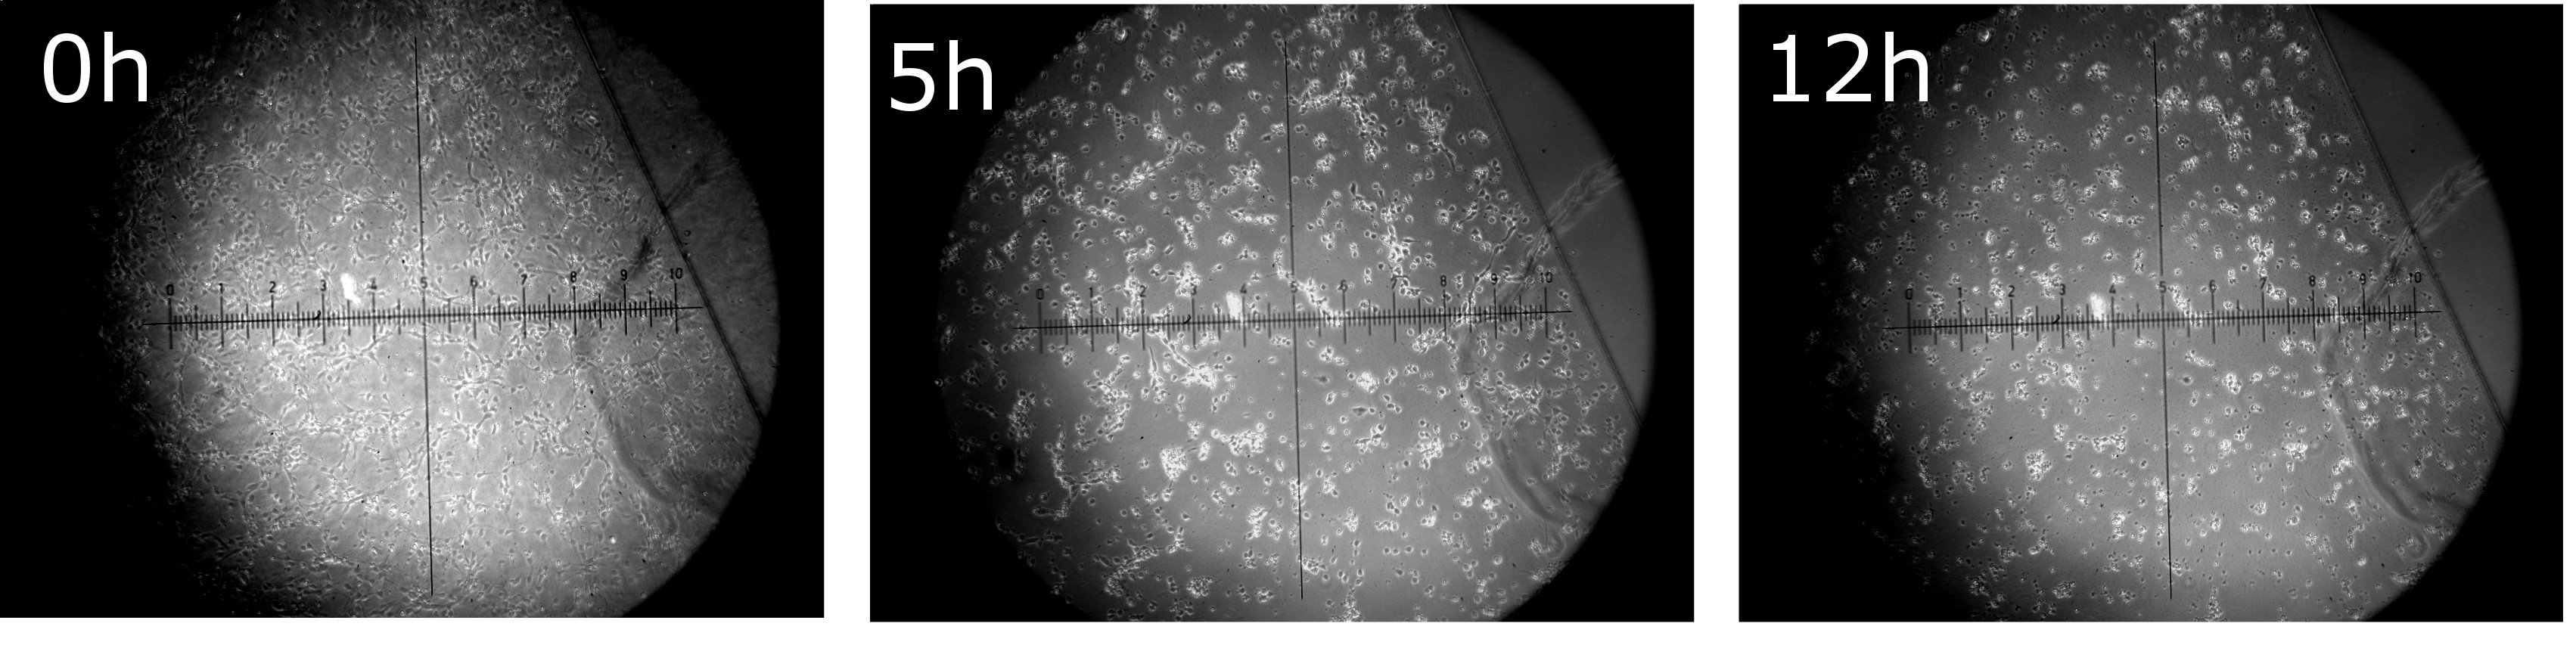
\includegraphics[width=15cm]{chapter4/figures/degenerationExample/degenerationExample.jpg}
            \caption[Time lapse of neuronal culture under steady microfluidic flow]{\textbf{Neuronal cultures exposed to steady flow lose their surface adhesion, retract their processes and degenerate after several hours.} Time lapse of a neuronal culture grown in the standard 1-layer microfluidic devices (section \ref{sec:devices:protocolDev}) placed under flow at 1 day \textit{in vitro}. The flow rate was \(1 \frac{nl}{s}\). Scale units: \(\approx100 \mu m\)}
            \label{fig:devices:degeneration}
    \end{figure}

    Initial experiments were conducted with the devices placed openly in the ambient environment while only plugged into a custom made heater system where heating resistors were brought into contact with the glass and the PDMS bulk and were controlled to \(37\degree C\) \cite{johnstoneThesis}. However, we had concerns as to how well this system controls the internal device temperature given that media at room temperature is pumped in. Additionally, maintenance of media CO\textsubscript{2} levels was based on connecting the pressure control system to a 5\% CO\textsubscript{2} / 95\% air gas supply. This configuration assured that the media in the flow reservoirs were fully CO\textsubscript{2} saturated but there was still a concern that as it travels through the tubes in the ambient air some CO\textsubscript{2} content could escape. To alleviate these issue, we built a custom made compact environmental chamber whose internal environment was controlled to \(37\degree C\) and 5\% CO\textsubscript{2} (figure \ref{fig:app:chamber}). The flow tubes were introduced into the environmental chamber through a small side hole before connecting to the devices. The tube configuration was purposefully selected such that the total tubing volume outside the environmental chamber was 3 times less than that of the internal tubing (\(\approx 16 \mu L\) vs. \(\approx 60\mu L\)). This meant that, while travelling from the reservoir to the device, the media spent triple the time inside the chamber environment than in the ambient one so any CO\textsubscript{2} lost outside would necessarily have been reabsorbed. We also calculated that the residence time inside the chamber is at least 10 minutes which is more than enough to heat the media to \(37\degree C\) given the micrometer scale of the tubing (this was verified with an inline flow thermocouple, PH-01, Multi Channel Systems). Nevertheless, the employment of the chamber did little to change the outcome of the flow experiments leading us to conclude that the basic physiological parameters of temperature and media CO\textsubscript{2} saturation did not play a major role in the degeneration.

    Since conditioning factors are known to exert a protective effect on neuronal culture \cite{kaech2006culturing,banker1980trophic} we explored the option of using conditioned media, i.e., media taken from a different culture for flow. We found that this had a pronounced effect on the cultures' tolerance in the sense that there was an initial flow period where the cultures' appearance did not seem to change. Additionally, even though fasciculation and degeneration still occurred, they developed much later, typically more than 10 hours into the flow session. Another interesting observation was that the rapid degeneration observed with fresh media flow seemed to occur regardless of the flow rate and presented itself even when the tubes were connected but the flow was set to \(0 \frac{nl}{s}\). These observations suggested that, when using conditioned media, a time window could be present where the culture is functional and useful experiments may be performed. They were also surprising in that the flow rate, i.e., shear, appeared to play a smaller than expected role in the adverse effects of flow. We therefore decided to conduct a systematic study to quantitatively assess the effect of conditioning and shear on the viability under flow and to establish what is the practical experimentation time window.


    \subsection{Quantitative viability analysis}
    \label{sec:devices:viabilityAssay}
    Analyzing how media conditioning affects viability under flow requires an analytic measure of conditioning. Since conditioning involves a continuous secretion of factors into the bulk media, it seemed plausible that, a conditioning scale would be proportional to the length of time which the media was in contact with the cells. We produced conditioned media by growing cortical rat cultures of prescribed densities in T-25 flasks with prescribed media volumes and without changing of the media. The precise protocol and the conditioning scale are provided in section \ref{sec:methods:cond}. Roughly, every 3 days of incubation in the flasks \textit{in vitro} are equivalent to 1 conditioning units.

    \begin{figure}[h]
            \centering
            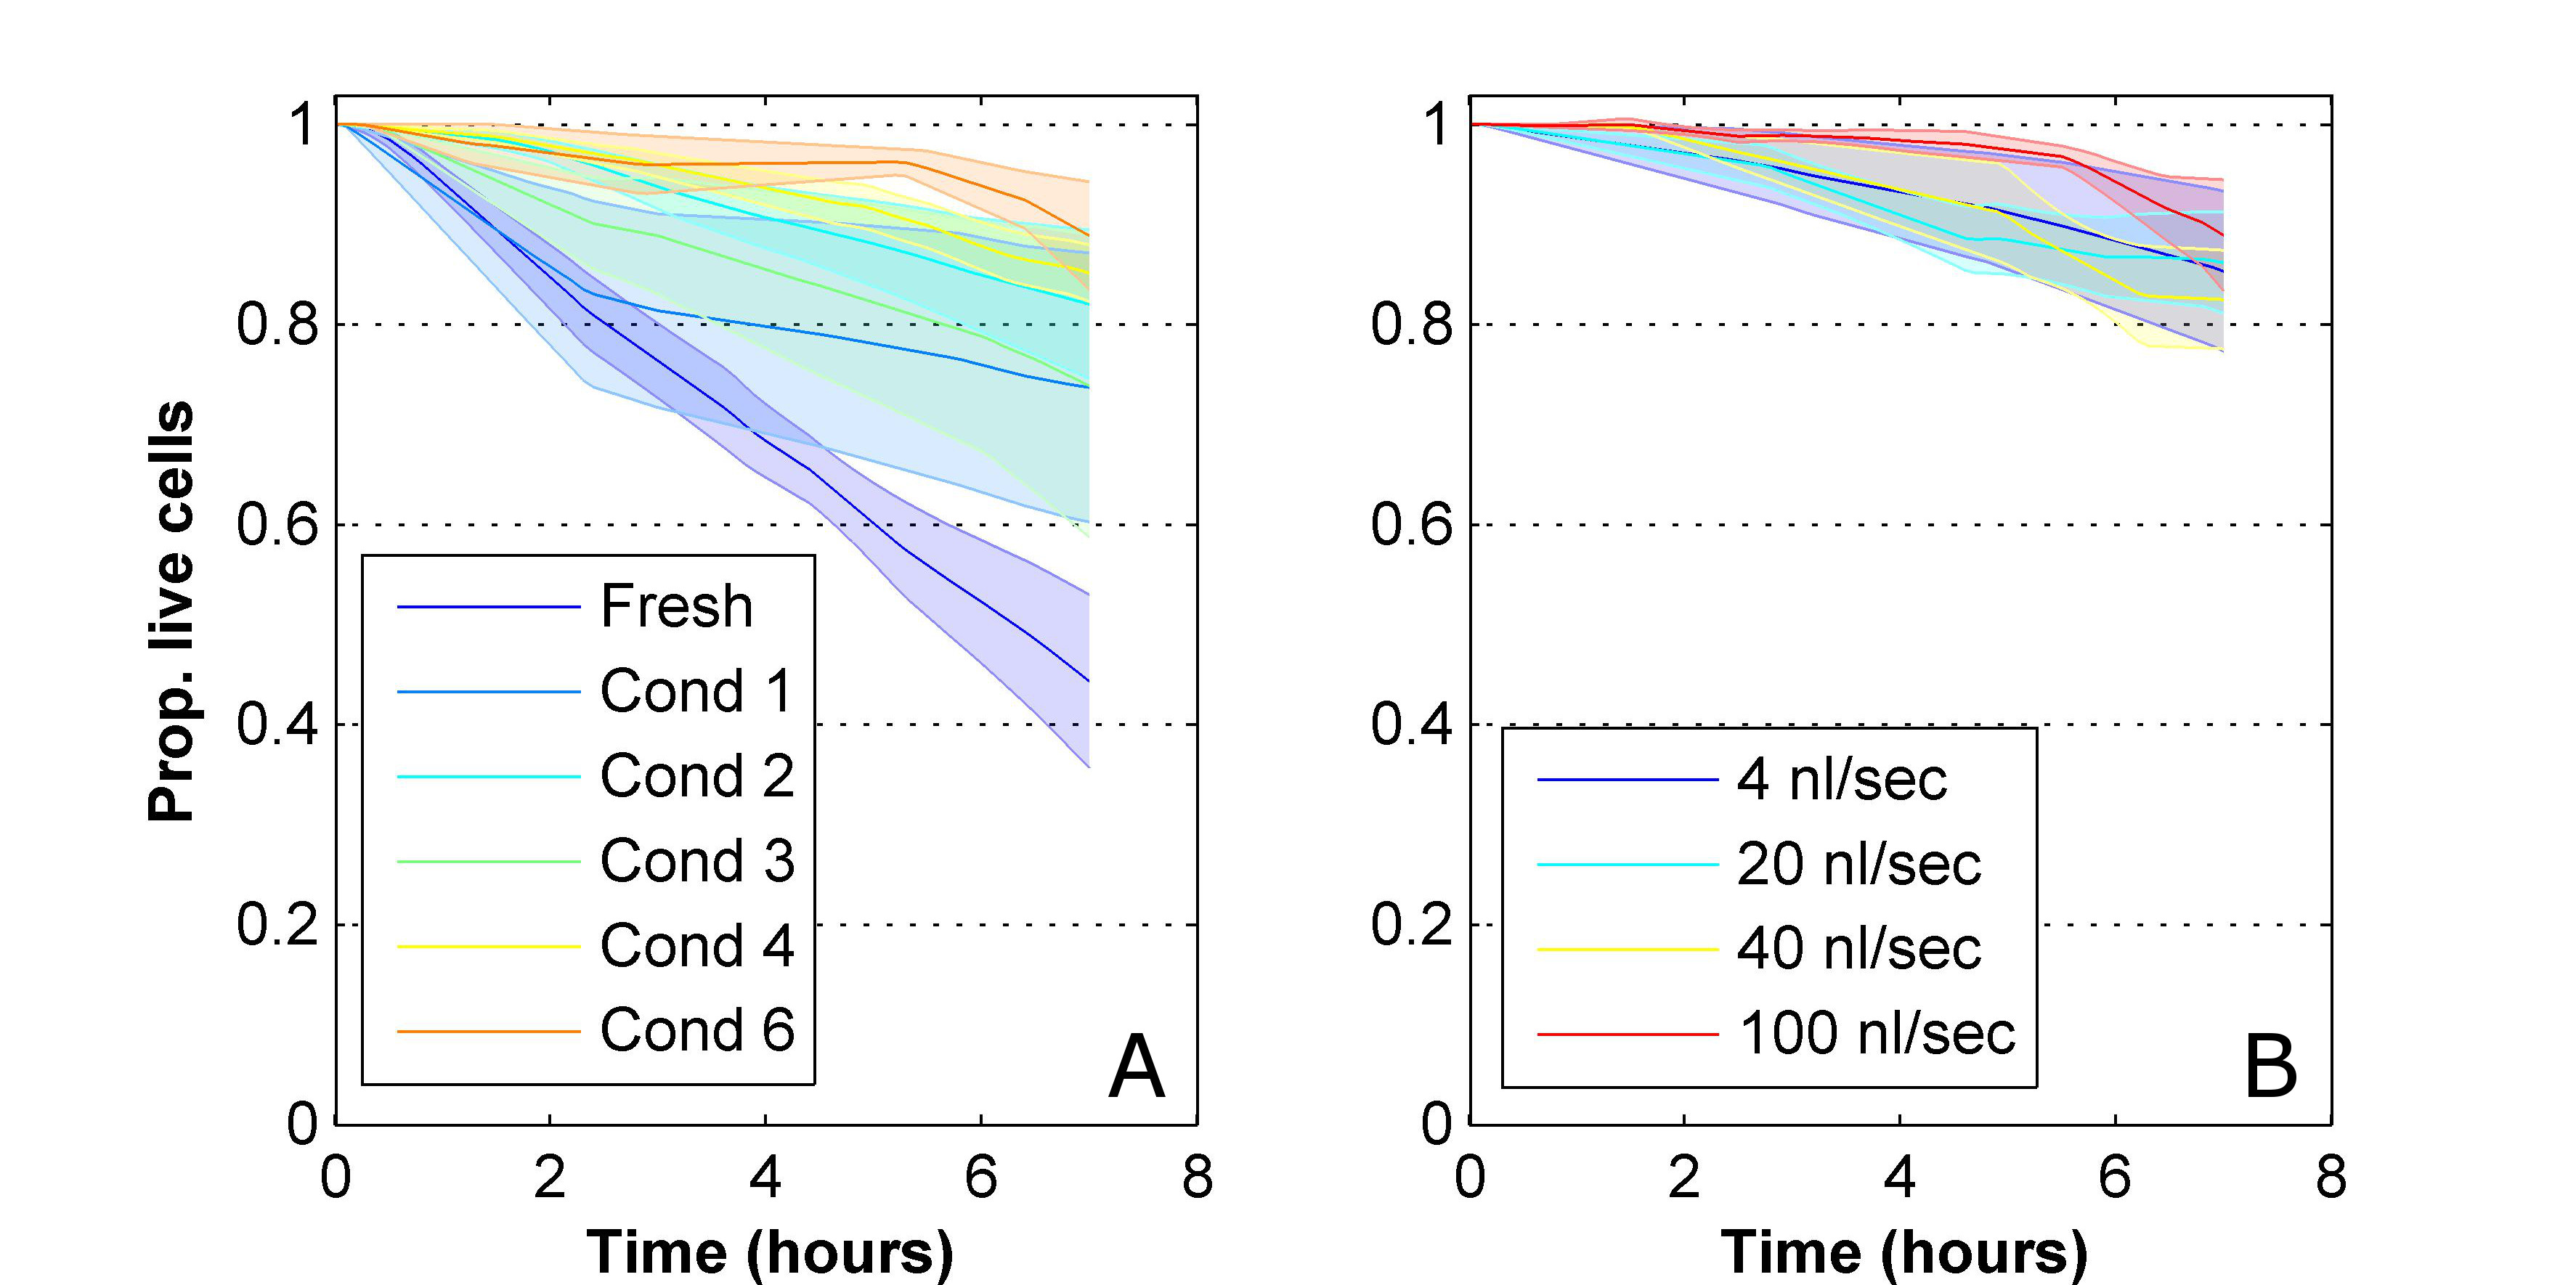
\includegraphics[width=15cm]{chapter4/figures/condImpression/condImpression.jpg}
            \caption[Effect of media conditioning and flow rate on viability of neuronal cultures under steady microfluidic flow]{\textbf{Using conditioned media for flow can significantly prolong the culture viability regardless of the flow rate.} (A) Averaged viability curves for flow with media of increasing conditioning levels. Every curve averages data from several flow experiments where a propidium iodide assay was used to quantitatively assess the number of dead cells over time (full description is given in full in section \ref{sec:methods:flow}). Example for such individual flow curves can be seen in figure \ref{fig:devices:viabilityDetAnalysis}. The flow rate for all experiments was \(40\frac{nl}{s}\). Shaded areas depict the SEM. (B) Averaged viability curves as in A but where the flow rates are varied whereas the conditioning level is fixed at 4. The data is based on 36 experiments from 9 platings. Every curve except for Cond 6 in panel A is the average of at least 3 experiments from 2 different platings. Cond 6 is based on 2 experiments from one plating.}
            \label{fig:devices:viabilityImpression}

    \end{figure}


    We ran a large set of steady flow experiments on macrocultures growing in standard 1-layer devices. The experiments were conducted in a range of conditioning levels and flow rates. To provide a quantitative measure of viability these flow experiments also included a propidium iodide assay (protocol and example in section \ref{sec:methods:flow}). In brief, propidium iodide was added to the flow medium so it was present around the cells for the length of the experiment. Intact plasma membranes of healthy cells are impermeable to this fluorescent DNA-binding molecule. However, when cells die their nuclear material becomes accessible and readily serve as a seed for propidium aggregation and therefore appears as a dot in fluorescent microscopy. These dots were counted to provide a quantitative measure of how many cells have died since the initiation of the flow. During a flow experiment fluorescent images were taken every 1-2 hours to generate a curve of the deterioration in viability. Figure \ref{fig:devices:viabilityImpression} shows averaged viability curves for a range of conditioning levels where the flow rate is fixed and for a range of flow rates where the conditioning level is fixed. The observations made in the previous section are clearly manifested in these curves: increasing of the conditioning levels is negatively correlated with the death rates whereas increase in flow rates within the tested range is not.

    \begin{figure}[!htb]
            \centering
            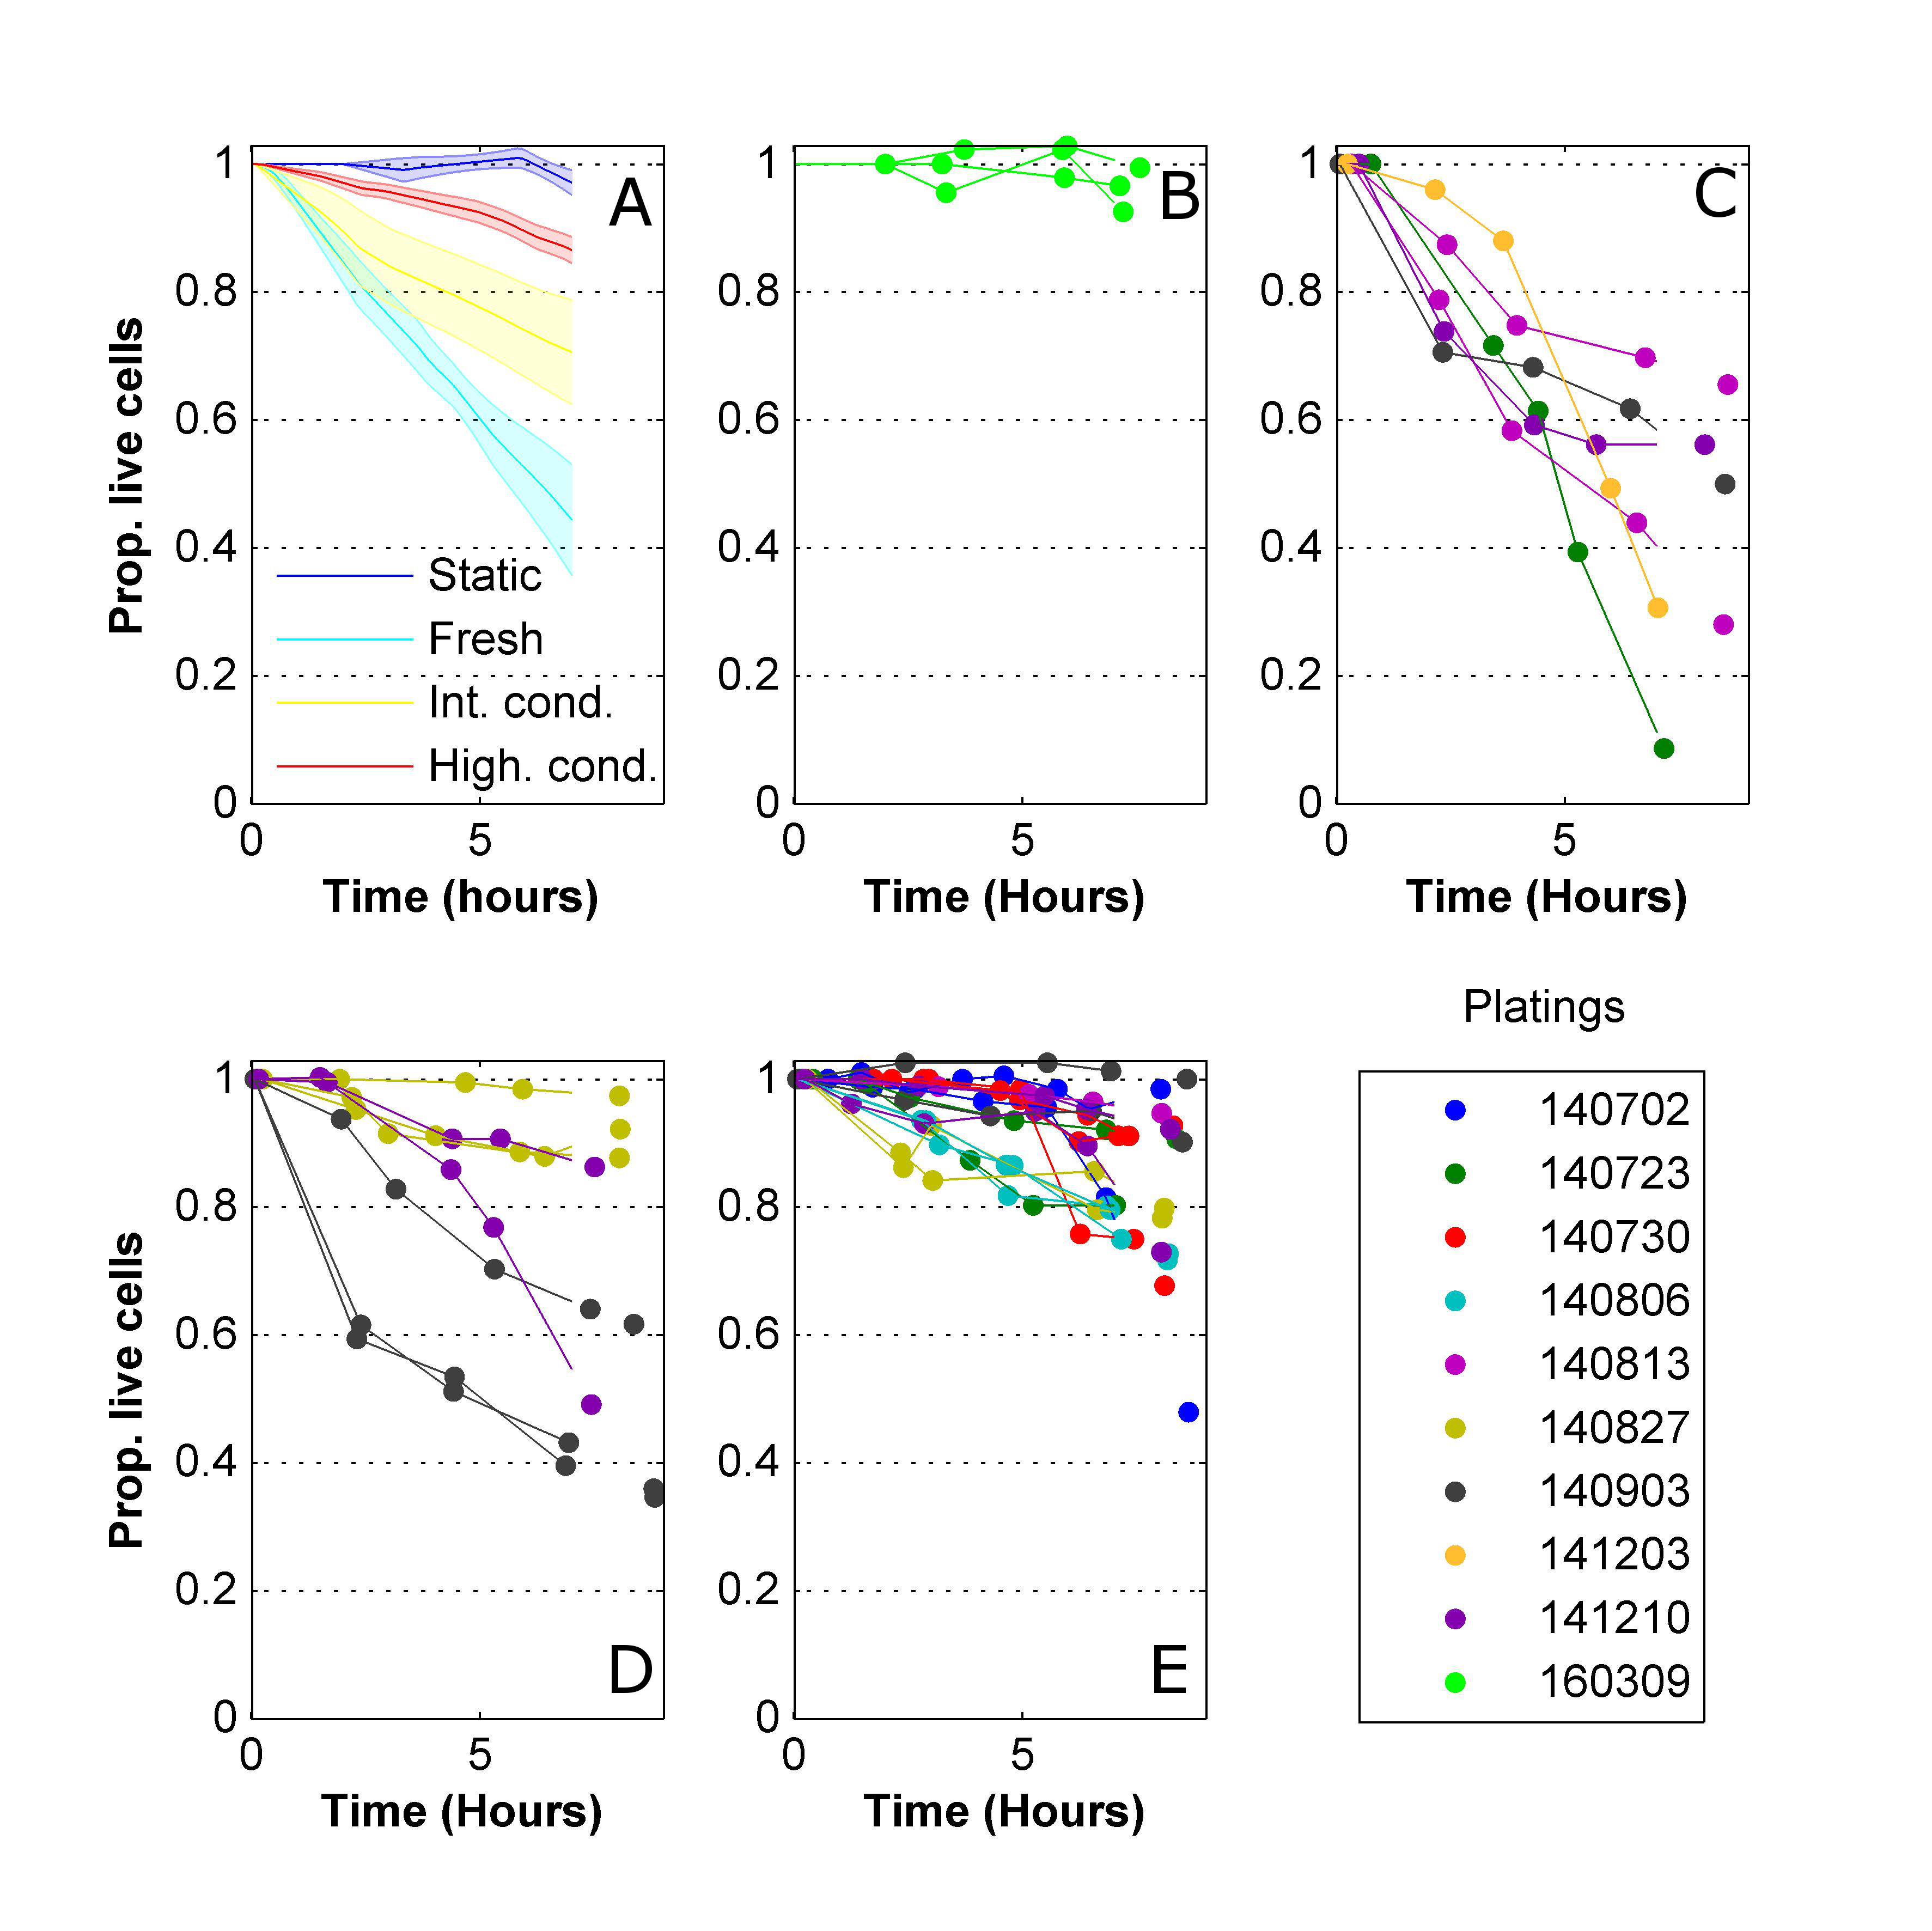
\includegraphics[width=15cm]{chapter4/figures/condDetAnalysis/condDetAnalysis.jpg}
            \caption[Example of viability curves from individual steady flow experiments]{\textbf{Individual viability curves do not exhibit any common temporal features so their average is linear.} (A) Averaged viability curves for increasing conditioning levels as in figure \ref{fig:devices:viabilityImpression} A but with a grouping applied to get improved separation (grouping specified in the text). The flow rate for all experiments was \(40\frac{nl}{s}\). An additional control curve is included where the devices were not connected to the flow system. (B-E) Individual viability curves from the experiments that were averaged in A. Each dot represents a fluorescent image where the number of dead cells were counted. The order of the panels B-E matches the order of the averaged curves as listed in the legend of panel A. Individual curves are color coded according to the date of plating of the given culture.}
            \label{fig:devices:viabilityDetAnalysis}
    \end{figure}



    To facilitate the statistical analysis we grouped the conditioning scale into 3 groups: Fresh media (same as before), intermediately conditioned (grouping conditioning levels 1 and 2) and highly conditioned (grouping levels 3-6). Figure \ref{fig:devices:viabilityDetAnalysis} shows the averaged viability curves generated with new grouping as well as a control curve made without connecting the cultures to the flow system at all (static). The figure also shows a breakdown of the averaged curves into the constituent individual ones per experiment. Since the individual curves did not exhibit any conspicuous common time dependent features and as the averaged curves were strikingly linear we reasoned that a fixed death rate model (linear) would be a plausible a description of this data. In accordance with this notion, the statistical analysis was based on fitting a line to the viability time series of each experiment with a forced intercept at (time=0, viability=1). The statistical testing was then performed on the fitted slopes and is discussed next.

    \begin{figure}[!htb]
            \centering
            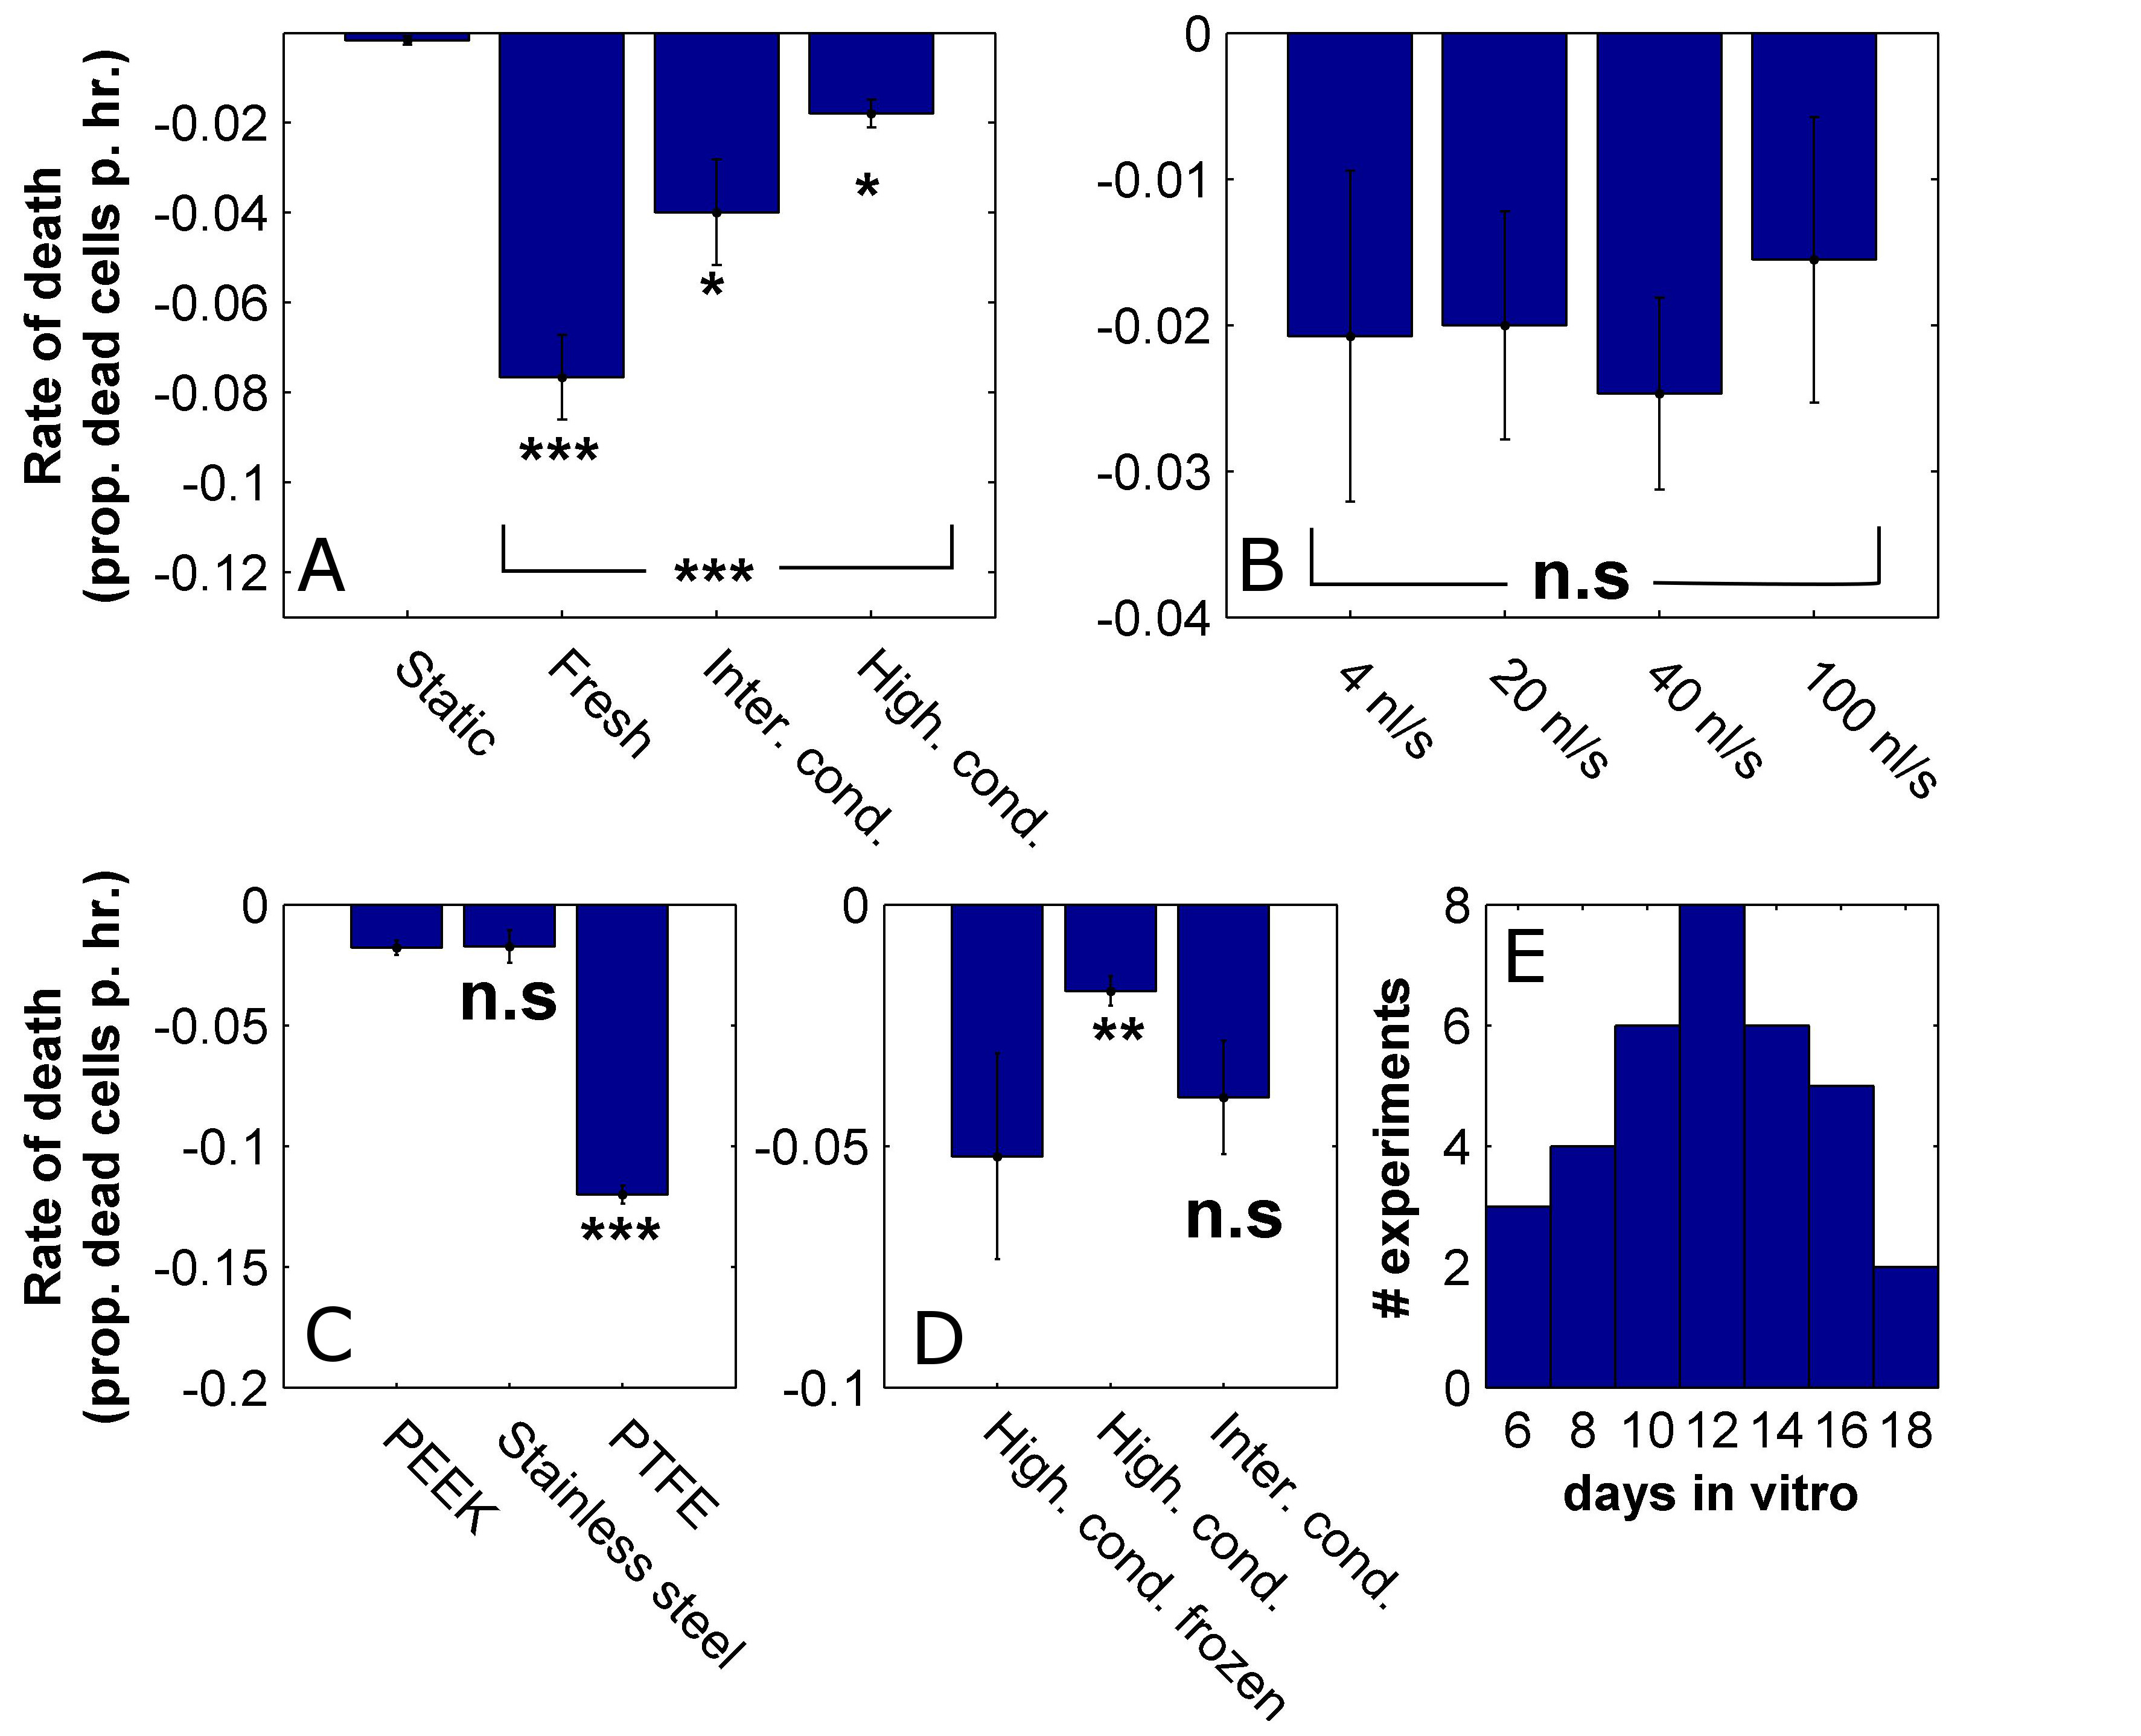
\includegraphics[width=15cm]{chapter4/figures/viabilityStats/viabilityStats.jpg}
            \caption[Statistics of death rates for various steady flow conditions]{\textbf{Death rates under steady flow depend on media conditioning levels and on the type of flow tubes but not on flow rates in the tested range.} (A) Comparison between the measured death rates under steady flow for increasing media conditioning levels and for control devices. Experiments were identical in all other parameters (flow rate \(40 \frac{nl}{s}\) and PEEK tubing). (B) Comparison between the measured death rates under steady flow for increasing flow rates (all highly conditioned media, PEEK) (C)  Comparison between the measured death rates under steady flow for different tube types (all highly conditioned media, \(40 \frac{nl}{s}\)). (D) Comparison between the measured death rates for conditioned media that was frozen and re-thawed and conditioned media that was directly used (\(40 \frac{nl}{s}\), PEEK). (E) Distribution of the ages of the cultures used in this study. The data is based on 49 experiments from 9 platings. Every bar is based on data from at least 3 experiments from 2 different platings except for the static data in panel A and the PTFE data in panel C which are each based on 3 experiments from one plating. Asterisks that group several bars indicate statistical significance of an ANOVA test. Asterisks next to individual bars indicate statistical significance of a t-test between the leftmost condition and the condition at hand. *, **, ***, n.s indicate statistical significance at a level of confidence of 95\%, 99\%, 99.9\% or \textless95\%, respectively.}
            \label{fig:devices:viabilityStats}

    \end{figure}


    Figure \ref{fig:devices:viabilityStats} shows a comparison of the fitted death rate slopes for various flow conditions. The conditioning levels of the flow media ware shown to have a significant effect on the death rate (Figure \ref{fig:devices:viabilityStats} A, 1-way ANOVA, \(p=1.5\times 10^{-5}\)). However, flow under all conditioning levels still resulted in death rates significantly higher than control (unbalanced t-tests, \(p=2.1\times 10^{-4}\), \(0.049\) and \(0.021\) for fresh media, intermediately conditioned and highly conditioned respectively). Thus were were not able to find a conditioning regime where the cultures were viable for long term under flow. To get an idea as to how much using conditioned media can extend the experimentation time, we calculated how long at least 90\% of the cells will be alive, given the established death rates. This provided times of 1.3, 2.5 and 5.6 hours respectively for the 3 conditioning levels at hand. Given that highly conditioned media was used, changing the flow rate did not produce a significant difference (Figure \ref{fig:devices:viabilityStats} B, 1-way ANOVA, \(p=0.91\)). The main experiments above were performed with PEEK tubing (see section \ref{sec:methods:flow}). We also tested if changing the tubing material would affect the viability under flow. We found that stainless steel tubing gave the same results as the PEEK for flow with highly conditioned media. PTFE tubing, however, was surprisingly associated with a significantly higher rate of degeneration (Figure \ref{fig:devices:viabilityStats} C, unbalanced t-tests, \(p=0.95\) and \(7.5\times 10^{-11}\) for stainless steel and PTFE tubing, respectively). Thus, the beneficial effect of conditioning seems to be absent when using PTFE. This could suggest that our PTFE tubing absorbs valuable conditioning factors or that it introduces contaminants into the media during flow. We did not further interrogate this non-trivial effect but it is important to make a note of how the tubing selection can affect these types of experiments. Finally, since all the conditioned media in this study was used straight from the culture flask we wanted to check whether it could be stored for later use as that would greatly simplify the experimental design. Consequentially, we extracted highly conditioned media, kept it frozen at \(-80\degree C\) for several weeks and then heated it back up to \(37\degree C\) prior to using it for flow. We found that the frozen media did not preserve the beneficial effects of the conditioning and resulted in significantly faster death rates as compared to the media used directly from the flasks (\ref{fig:devices:viabilityStats} D, unbalanced t-test, \(p=0.0073\)). Interestingly, the performance of the frozen media was statistically the same as that of the intermediately conditioned media (unbalanced t-test, \(p=0.59\)) so the benefits of conditioning were still partially present. It is likely that some of the conditioning factors degrade over time and are sensitive to freezing and thawing (e.g., large protein molecules) hence the above results.


\section{Chapter conclusion}
     \label{sec:devices:conclusion}
     In this chapter, we demonstrated a capacity for growing rat macrocultures (standard size) and microcultures in microfluidic devices. The observations made in sections \ref{sec:devices:circulation} and \ref{sec:devices:microcultures} highlight the challenges that exists in the design of microfluidic devices for neuronal culture in finding a `goldilocks' circulation regime. On one hand, enough nutrients and oxygen need to be allowed into the device to meet the requirements of the culture and, on the other hand, conditioning factors must be prevented from `escaping' as they are required for sustaining the development. The precise design is strongly dependent on the size and density of the culture as these inform its oxygen and nutrient requirements and also the secretion rate of conditioning factors.

     In the second part of this chapter we used a viability assay to quantitatively observe the cultures' health under flow. We found that using highly conditioned media can sustain the viability of the culture for several hours under flow and therefore consider it a promising approach for establishment of the system. Interestingly, the shear rate induced by the flow did not correlate with the viability which suggests that the deleterious effects are mediated solely by removal of conditioning factors and not at all by physical shear. Nevertheless, this is not the only possible interpretation for these results. A related study testing the viability of neuronal culture under a range of flow rates reported a shear threshold associated with culture degeneration \cite{liu2013galanin}. This study found that a compound isolated from brain tissue named Galanin protects the cultures from the shear so that, when it is introduced into the flow media, an effective increase in the degeneration threshold is observed. A possible interpretation of our results could therefore be that the conditioned media contains factors similar to Galanin that protect the cells from the shear and therefore effectively increase the flow rate threshold to a level exceeding the tested range. The study presented here cannot unambiguously distinguish the above-described narratives. This issue will be further addressed in the next chapter where electrophysiological measurements under flow will be presented and shed light on the mechanisms by which flow interacts with the culture.




%\chapter{Neuronal activity under steady microfluidic flow}
\label{chap:activityAndFlow}

\section{Introduction}
In the previous chapter, we found that when using conditioned media for flow the cultures' viability may be prolonged so as to allow conducting of useful experiments. The viability assay used, however, is a crude measure of neuronal functionality and indicates that a cell has died only at late stages of apoptosis / necrosis, after the plasma membrane had been breached. This Ph.D work is concerned with how volume transmission interacts with network activity and plasticity so electrophysiological measurements are the most relevant measure of functionality. Although in the previous chapter we found that shear stress was not the major determinant of neuronal viability there was still concern that shear effects would be manifested in the activity. Thus, in this chapter, beyond characterizing the effects of media conditioning, we also include experiments varying flow rates and monitoring the activity of the cultures in device bonded to MEAs. In addition, we tested a semi-permeable membrane that would allow passage of small molecules, but act as a barrier to de-couple the flow from the cells as we hypothesized that this approach could potentially reduce both factor removal as well as shear stresses. Finally, we introduce here an additional parameter of culture age as this eventually was found to be critical for the success of this approach.

\label{sec:crossFlow:intro}

\section{Neuronal cultures in cross flow devices on MEAs}
Figure \ref{fig:crossFlow:crossFlowIllustration} shows the devices used for the experiments conducted in this chapter. We extended the design of the basic microfluidic channels used in the flow study in chapter \ref{chap:devicesAndFlow}, to allow the incorporation of a semi-permeable membrane. To accommodate the membrane (Whatman cyclopore, \(100 nm\) pore size, cat. no. 7060-4701), they comprised a flow and cell layers which were joined either to each other or to the membrane from each side, depending on the experiment. Because of the perpendicular arrangement of the flow channel in relation to the cell channel the devices were tagged `cross flow'. Since assembly of such multi layered devices through plasma bonding is problematic and since plasma bonding of PDMS to the commercial MEAs could damage the surface and is not practical for re-use, we opted to use the tape technology (section \ref{sec:devices:bonding}). Thus prior to device placement, the MEA surfaces were treated with PEI (section \ref{sec:methods:surface}). In parallel, the device layers were cut out of the \(125 \mu m\) silicone transfer tape and aligned using a custom made alignment tool (essentially comprising two pegs holding the layers in place through alignment ports). The assembled devices were oven sterilized and joined with the MEA surfaces, after these have been washed and dried from the PEI solution. The devices were manually aligned to the MEAs in such a way that the intersection area between the flow and cell channels was on top of the central electrode pads area.

The media formulation described in the previous chapter as `highly conditioned' was found in preliminary experiments to be inadequate for electrophysiology under flow as it gave rise to inconsistent results and generally to silencing of most of the activity. Thus, the experiments in this chapter are predominantly based on using conditioned media which is simply the bulk media of the same culture dish (i.e., media which the particular tested culture grew in, termed `self media') and this approach was the one that finally gave usable behaviour. Nevertheless, how flowing with media from other culture dishes (as was the case in the conditioning protocol of the previous chapter) affects the activity was also explored. These data will make it clear why self media is a better approach than the conditioning protocol from the previous viability studies and will be directly addressed in the conclusion of this chapter. Since self media is extracted directly from the tested sample we increased the volume of growth media to \(4 ml\) per sample to make sure that enough supply would be available for the flow session. We used custom made glass cylinders which were glued to the MEA following the attachment of the devices to hold the media (figure \ref{fig:pulses:circularIllustration}).

 \begin{figure}[h]
       \centering
       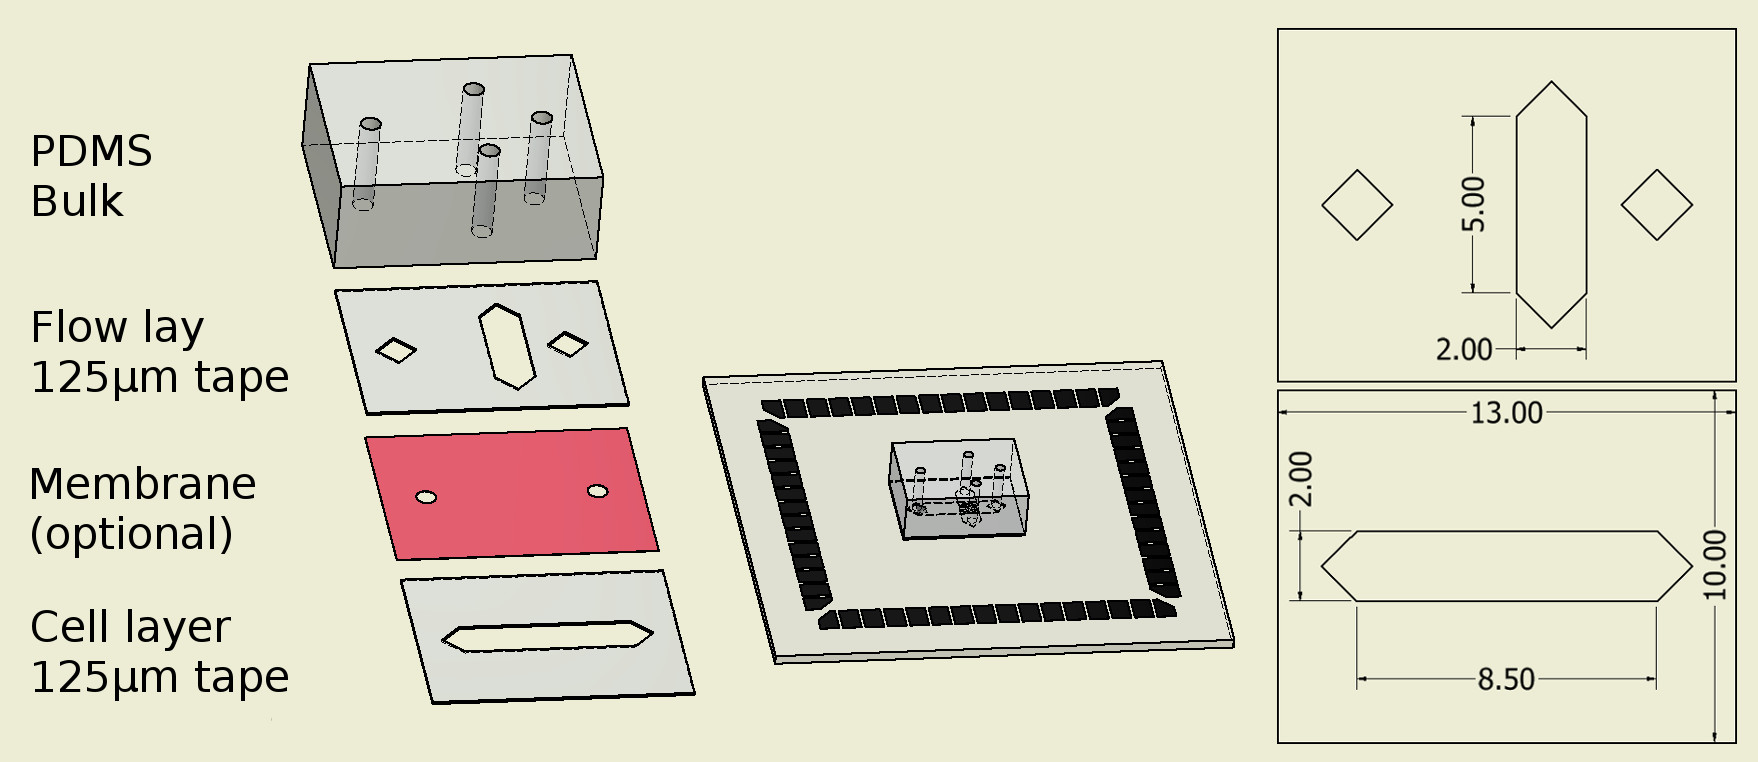
\includegraphics[width=12cm]{chapter5/figures/crossFlowIllustration/crossFlowIllustration.jpg}
       \caption[Illustration of the cross flow devices used for measuring culture activity under flow]{\textbf{Illistration of the cross flow devices.} Illustrations showing the constituent layers of the device laid out as well as assembled and joined to an MEA. The semi-permeable membrane is optional and shown in red. The dimensions of the flow and cell layers are also shown in millimeter units. Further details about the device fabrication are found in the text.}
       \label{fig:crossFlow:crossFlowIllustration}
  \end{figure}

To seed the cross flow devices, the flow channel ports were blocked so as to prevent seeding solution from being diverted through the flow channel. The seeding volume was \(3 \mu L\) which is enough to fully saturate the cell layer (\(\approx 2 \mu L\)). The seeding density was \(7\times 10^6\frac{cells}{ml}\) which was calibrated to achieve an area density of \(\approx 1000 \frac{cells}{mm^2}\) in the central electrode pads area. Cultures seeded in such devices typically developed well for over a month. This contrasted with the standard 1-layered devices introduced in section \ref{sec:devices:protocolDev} where many of the cultures did not develop past the end of the 3\textsuperscript{rd} week. This could be attributed to the increased volume of the cross flow devices which would be associated with improved nutrient and by product circulation or to the switch to PEI surface treatment which is considered better for neuronal adhesion. Maintenance of the seeded devices was as described in \ref{sec:methods:culture} and follows the protocol achieved in section \ref{sec:devices:protocolDev}.



  \begin{figure}[!htb]
       \centering
       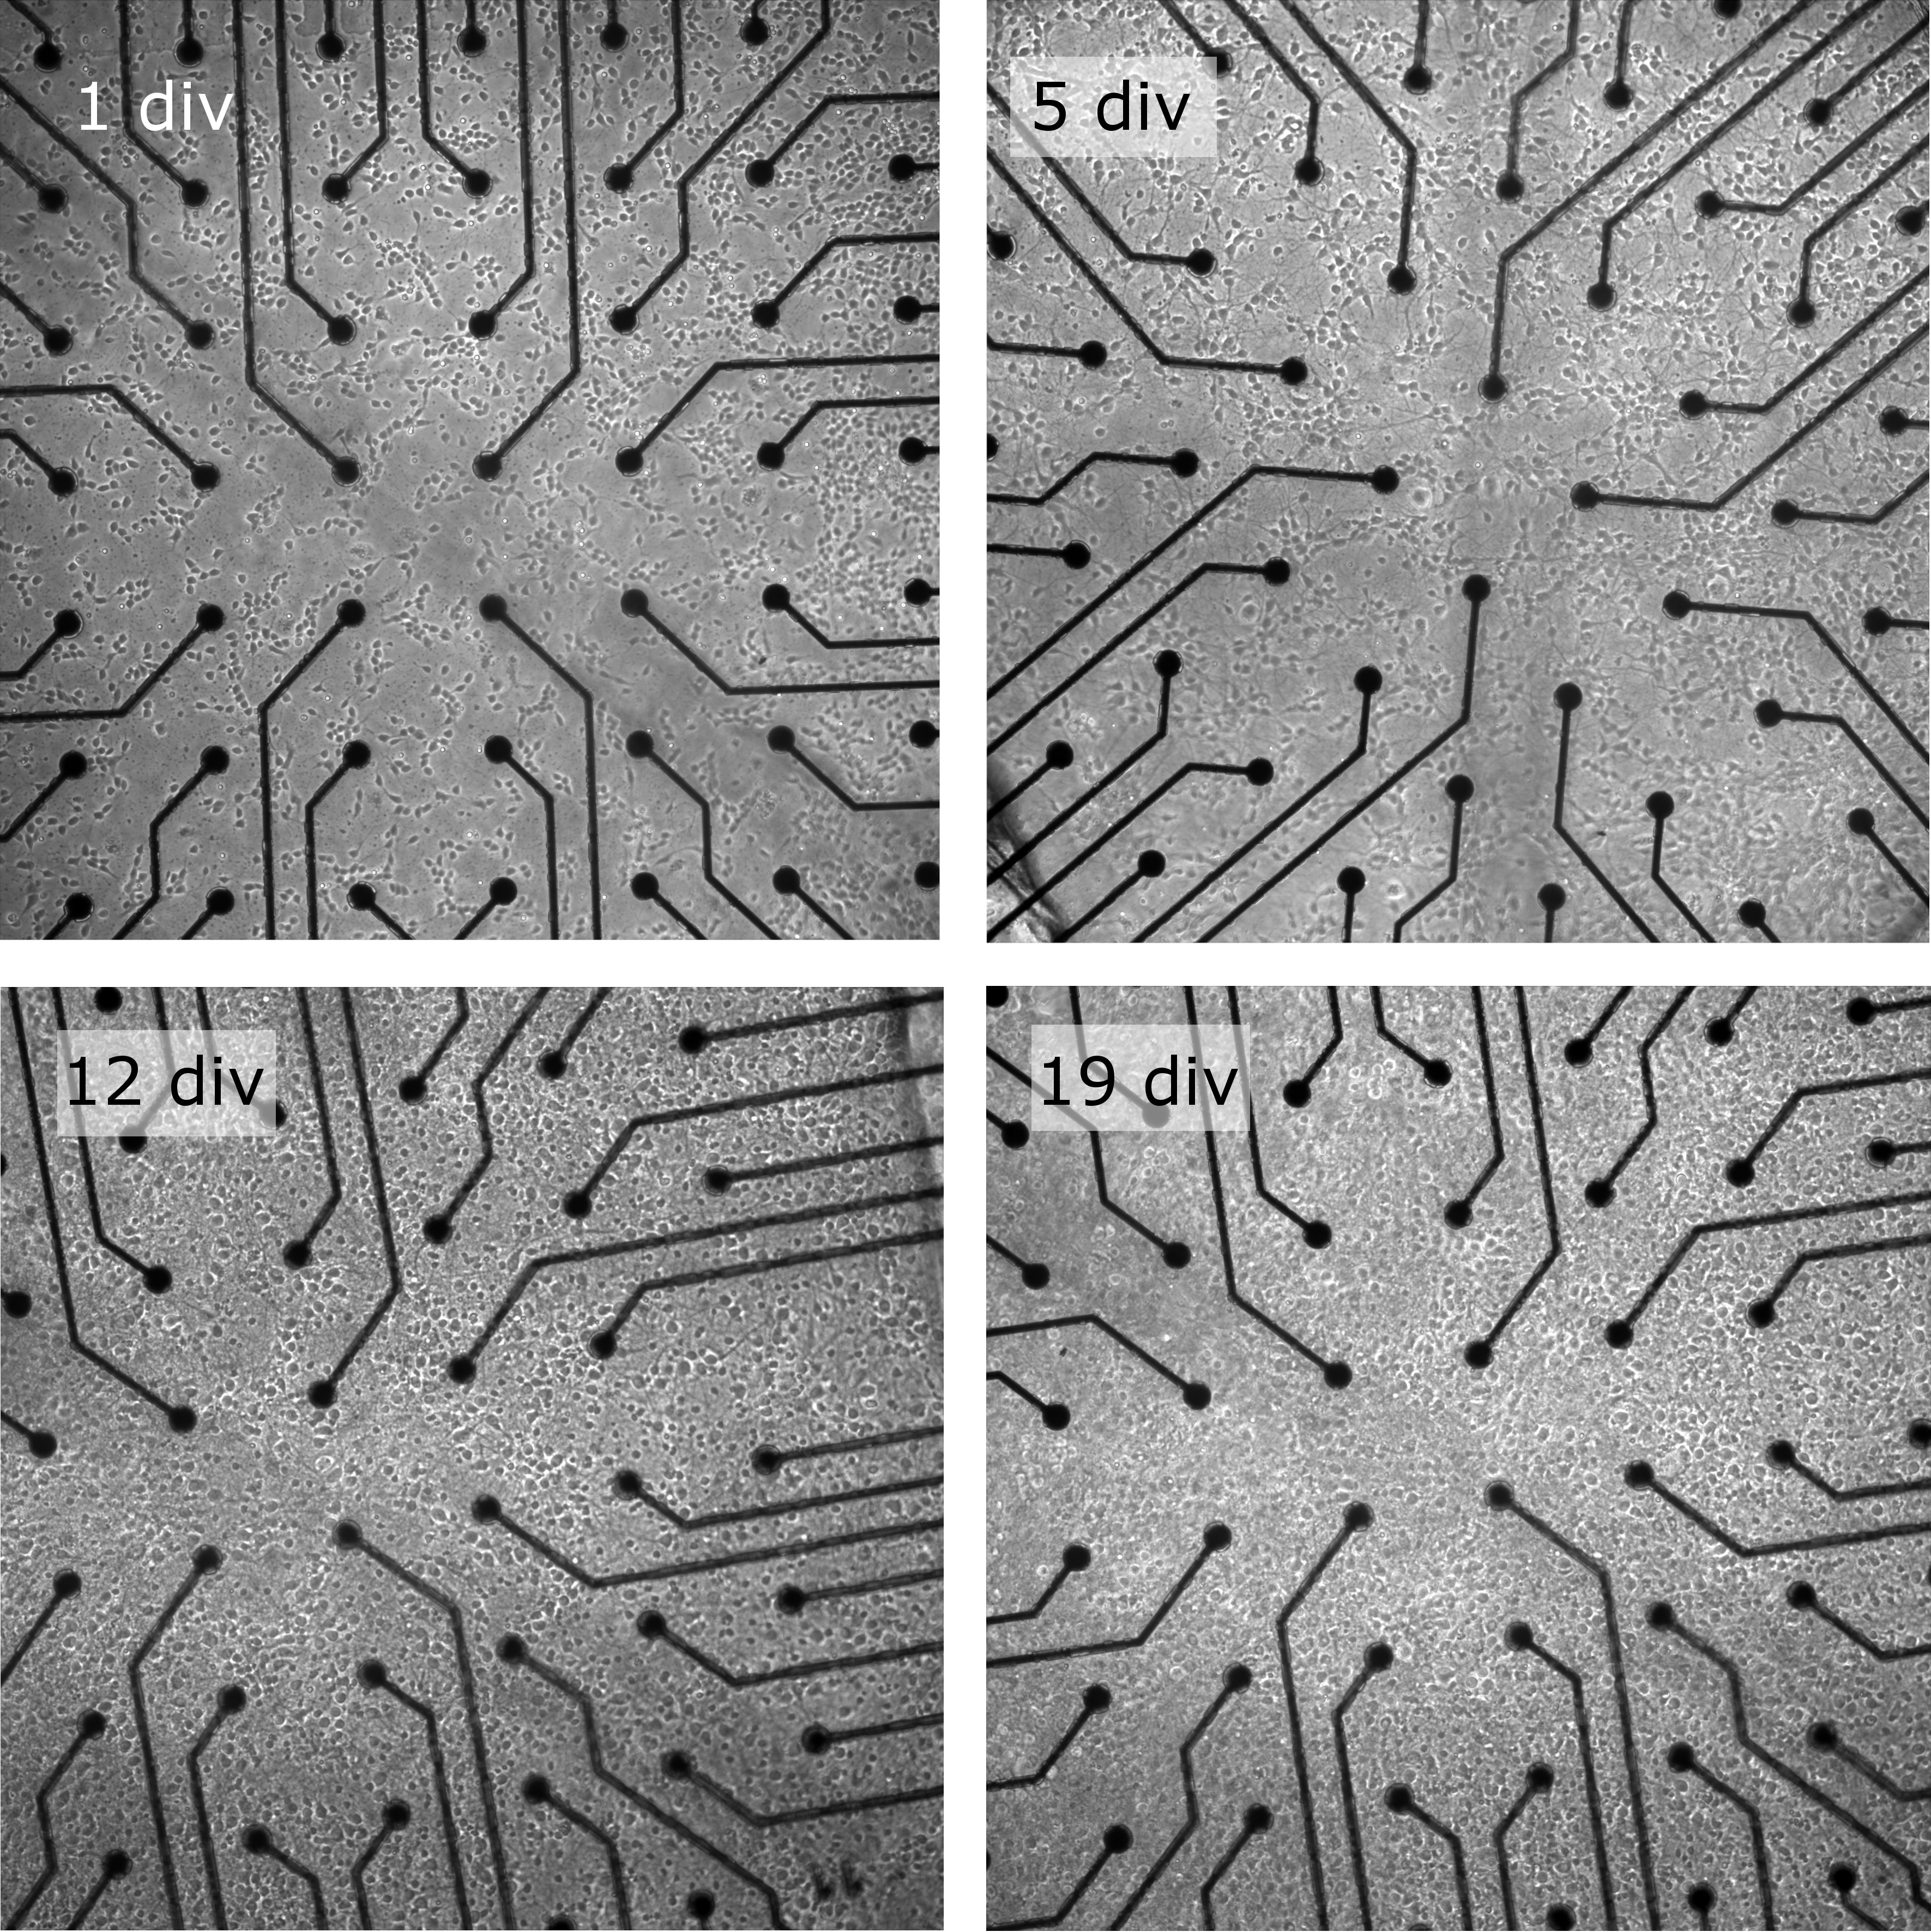
\includegraphics[width=15cm]{chapter5/figures/crossFlowDev/culture.jpg}
       \caption[Images of a neuronal culture growing in cross flow devices]{\textbf{Neuronal cultures develop well in cross flow devices for over 3 weeks \textit{in vitro}.} Images of neuronal culture growing in the cross flow devices at several developmental time points. The images were taken in the area of intersection between the flow and cell channels. The electrodes are spaced \(200 \mu m\) apart for length reference.}
       \label{fig:crossFlow:crossFlowDev}
  \end{figure}


\section{Activity under flow for 2 weeks old cultures}


        The first set of experiments were performed on cultures at ages 12-15 days \textit{in vitro} (i.e., 2 weeks). These experiments utilized direct flow (i.e., no membrane). This age range is similar to the one used for the viability study in section \ref{sec:devices:viability}. The recordings in this chapter were all performed in the presence of electrical stimulation in the form of a single test pulse delivered to a single MEA electrode every 5 seconds. The stimulating electrode and the pulse voltage amplitude were selected before the experiment so that an observable network response would be elicited by the stimulation. The reason for using stimulations is twofold: firstly, spontaneous activity is known to be inherently volatile as it probably depends on stochastic processes of intrinsic excitability and synaptic noise. Since the aim of these experiments is to identify conditions where the activity is stable we were concerned that variability associated with spontaneous activity would be confused with the destabilizing effects of flow. Thus, we reasoned that electrical stimulation which is more deterministic than spontaneous activity might be a more adequate basis for assessing the stability under flow. Secondly, the ability of neuronal ensembles to respond to stimulation underlies their facility for representing and transforming external information. We therefore found it is important to include a criterion where the response to stimulation would be maintained under flow. Since under our stimulation regime background spontaneous activity is also present between the stimulations, we also presented the data using raster plots (e.g., figure \ref{fig:crossFlow:slowFastExample} A). Thus the presence of stimulations should be taken into account when referring to these data.

        The extracellular recordings and data analysis pipeline as well as the stimulation protocol are specified in section \ref{sec:methods:MEARecording} and have been further described in sections \ref{sec:activity:spontActivity} and \ref{sec:activity:evoked}. All the experiments described in this chapter were initiated with a 30-60 minute period of baseline recording before the sample was plugged into the flow system. Where self media was used, it was withdrawn from the sample and flushed through the system after the baseline recording.

        \subsection{Effect of flow rate}
        \label{sec:crossFlow:slowFast}
        We found a strong flow rate dependent effect on the activity which is exemplified in figure \ref{fig:crossFlow:slowFastExample} which shows baseline as well as slow and fast flow data for a young culture. In the baseline recording, the culture exhibited synchronized bursting dynamics which are typical for rat cultures of this age (sections \ref{sec:activity:spontActivity} and \ref{sec:activity:mouseRatComp}). These synchronized dynamics were manifested in vertical lines in the raster plots and with high values of correlation throughout the correlation matrix. Additionally, the culture responded to test stimulation pulses with a network reverberation, although these sometimes failed to appear. Immediately upon initiation of the fast flow, these synchronized dynamics broke down with the neurons initially switching to a fast tonic firing and then gradually becoming silent. The tonic firing was manifested in a dramatic reduction in the correlation values. Additionally, the stimulation response was all but completely abolished with the activity not occurring preferentially after the stimulation but tonically spread in the observed time window (figure \ref{fig:crossFlow:slowFastExample} B). Remarkably, even the direct responses (low latency, low jitter responses appearing as straight lines in the response rasters) were abolished under flow which suggests that the basic biophysics of the neurons had been compromised. Under slow flow, there was no sign of these dramatic perturbations to the activity. Indeed, slow flow induced some temporary perturbations to the activity (e.g., the stimulation responses were temporarily reduced) but these faded within minutes. Overall the synchronized bursting dynamics and the stimulation responses were maintained and the structure of the correlation matrix was preserved.

        \begin{figure}[!htb]
            \centering
            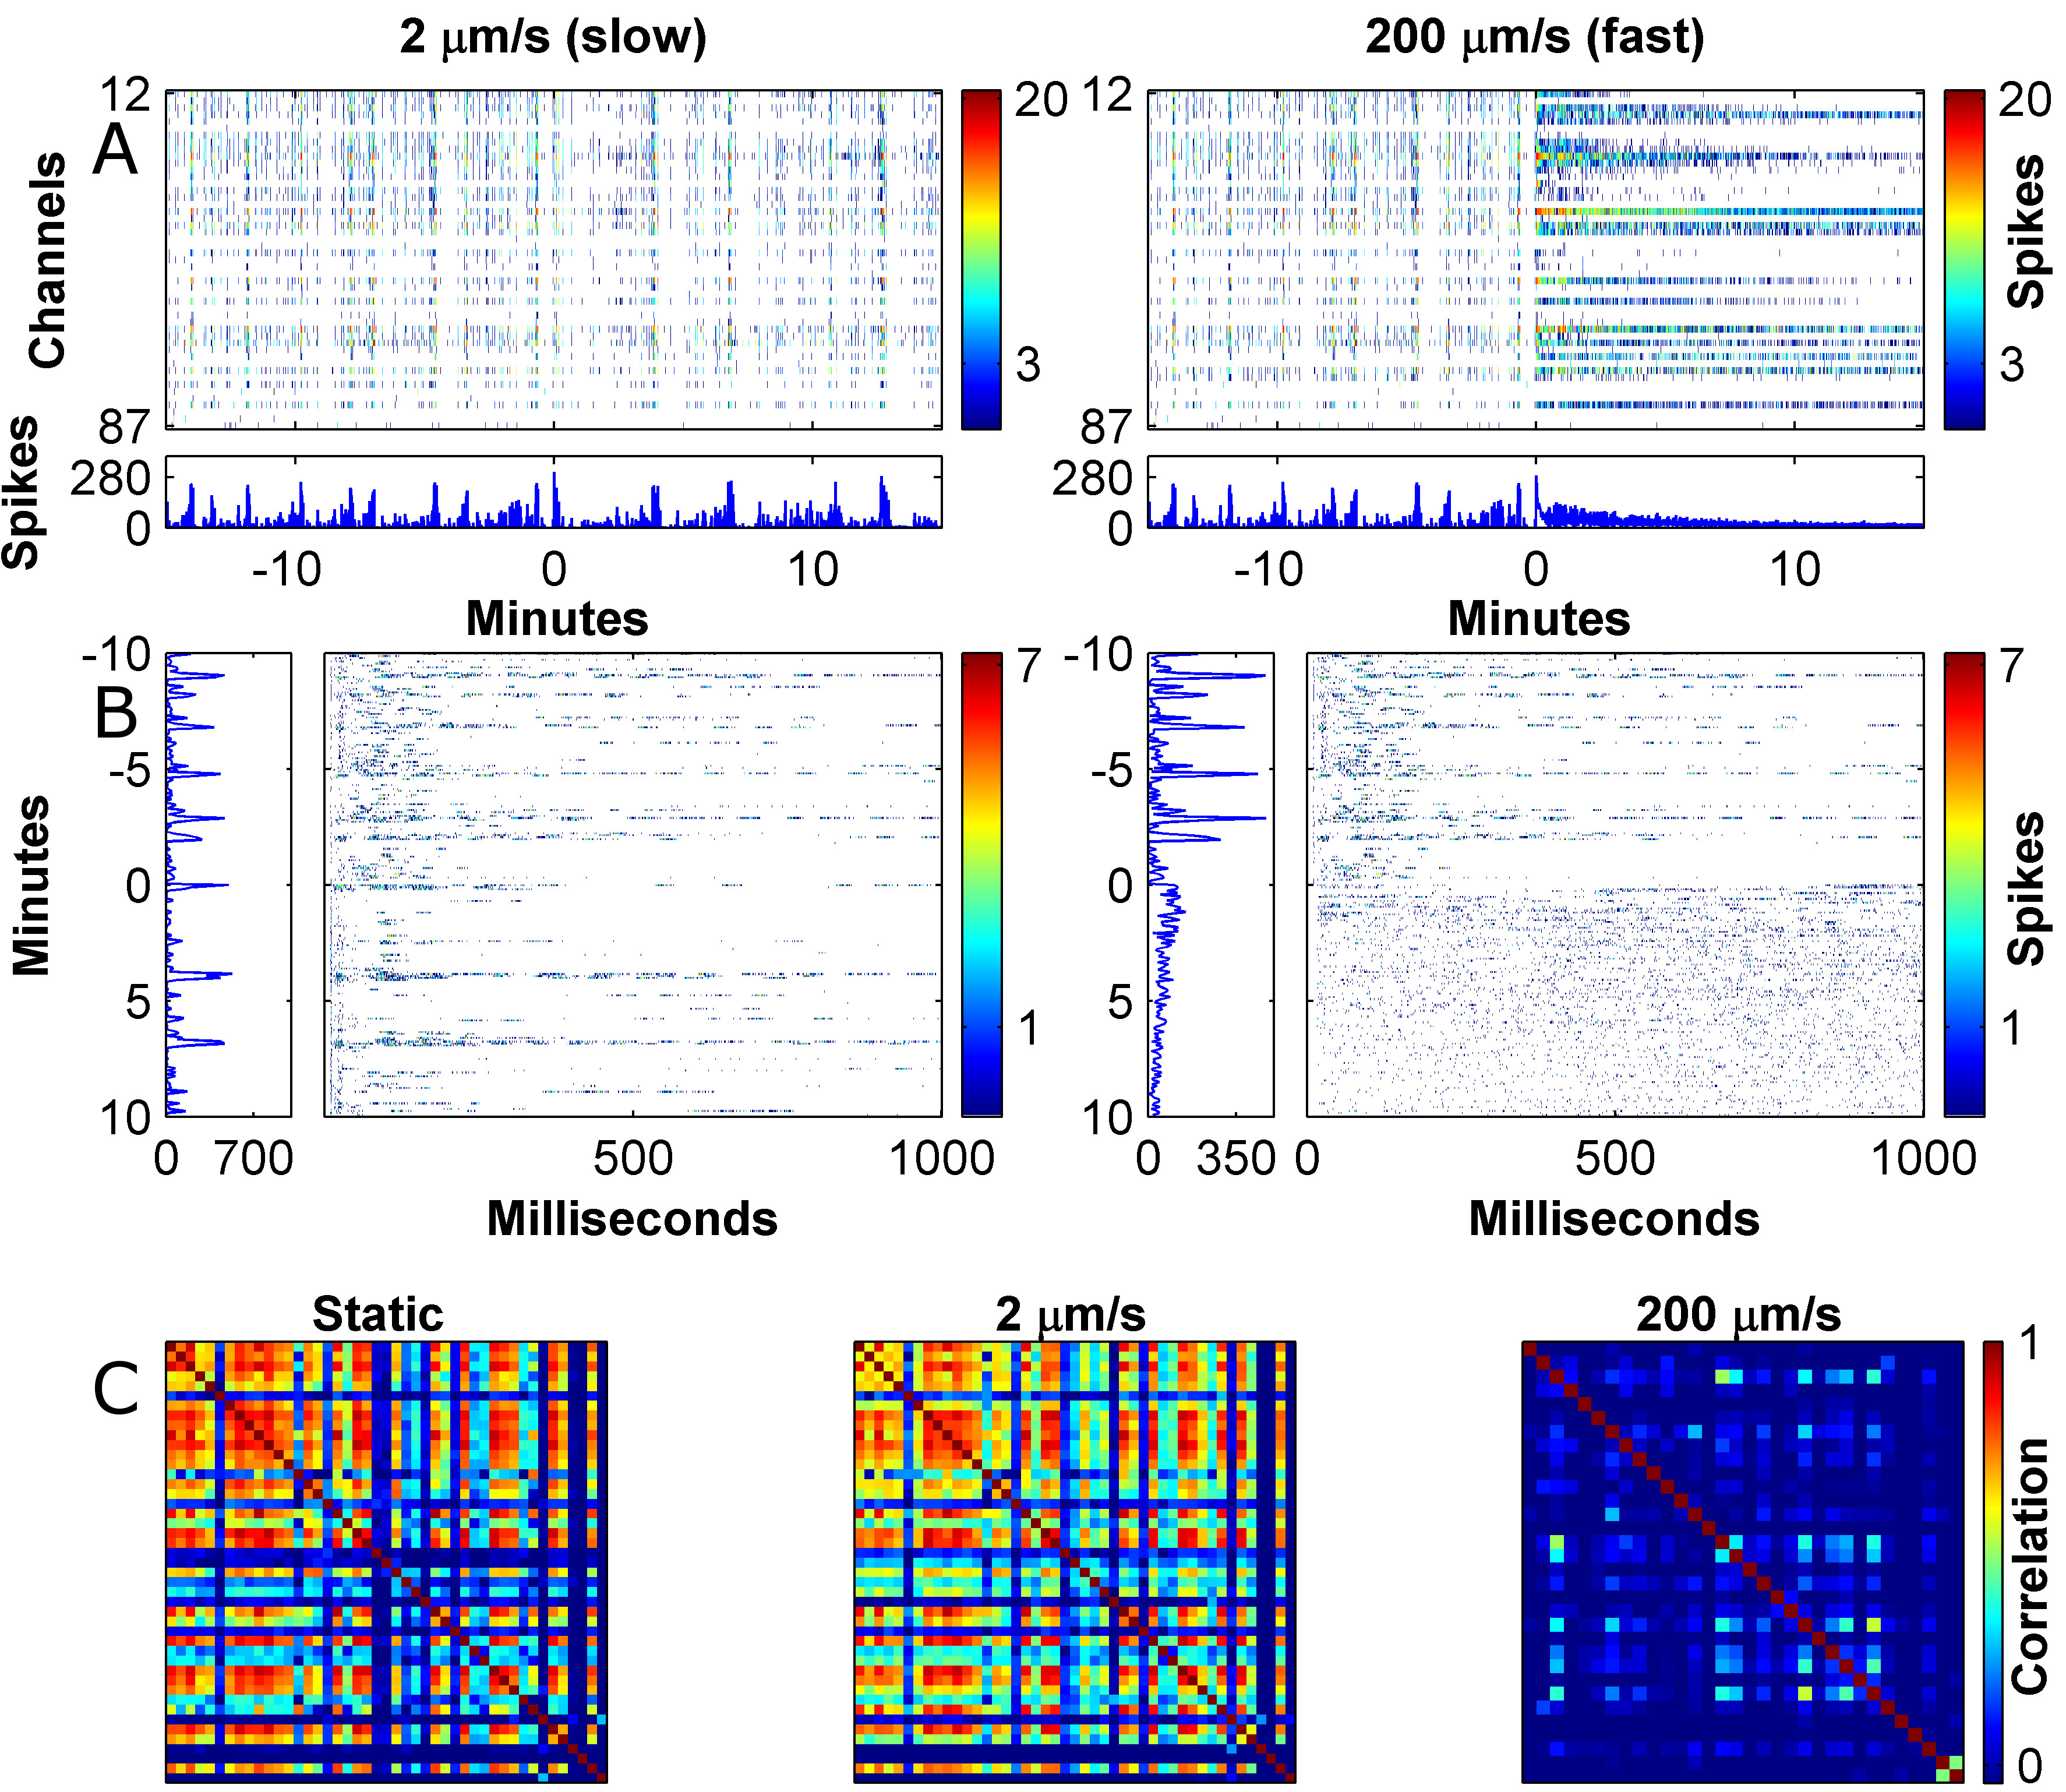
\includegraphics[width=14.5cm]{chapter5/figures/slowFastExample/slowFastExample.jpg}
            \caption[Example for the Effect of flow rate on the activity of a young culture under flow]{\textbf{Young cultures placed under flow with self media suffer a flow rate dependent disruption to the activity.} (A) Network raster plots showing the activity of the culture before (negative times) and just after (positive times) initiation of slow and fast flow (left and right panels, respectively) in \(500 ms\) bins. These raster plots show activity under electrical stimulation (test pulses at \(0.2Hz\)) and therefore represent combined spontaneous and evoked activity. Note the immediate switch to a tonic and desynchronized regime in the case of the fast flow. (B) The culture's network responses to stimulation before and just after initiation of slow and fast flow. Note the immediate loss of the temporally localized stimulation response in the case of fast flow. Response raster plots use \(1 ms\) bins. (C) Correlation matrices representing the culture's activity in static conditions and under flow. All matrices are based on 10 minute activity samples. In the case of flow the samples were taken 15 minutes into the flow session. To obtain the shown data, the culture was initially recorded for 30 minutes in baseline conditions following which the flow tubes were connected and 20 minutes of slow flow were recorded. The flow was then increased to the fast rate for the remainder of the session. This experimental sequence was an exception which was made to observe different flow rates applied to the same culture. In the typical case (figure \ref{fig:crossFlow:slowFastStats}) slow and fast flow regimes were conducted in separate experimental sessions.}
            \label{fig:crossFlow:slowFastExample}
        \end{figure}

        To make sure that the phenomena reported above were indeed consistent we ran several such experiments with slow and fast flow rates and show the statistics in figure \ref{fig:crossFlow:slowFastStats}. The results are presented through 3 measures: global firing rate (i.e, total number of spikes recorded over all electrodes), mean correlation (i.e., the mean of the correlation matrix without the diagonal elements) and stimulation response ratio.

        Stimulation response ratio refers to the ratio between the total spike count (over all electrodes) in a \(200 ms\) window just following the stimulation and a window of the same size 2 seconds later. The reason for this definition is that a measure that counts only the spikes following the stimulation is very sensitive to the background spontaneous activity. Thus we employed a second window at a distance from the stimulation under the assumption that its spike count is attributed solely to spontaneous activity. The ratio measure therefore represents the relative increase in  firing rate due to the stimulation relative to the ongoing spontaneous activity. As some of the conditions used here caused large changes in intensity and temporal distribution of the spontaneous activity, using a simple stimulation response measure would have been meaningless. The firing rate and stimulation response ratios are further normalized to the baseline values of these measures (i.e., from the baseline recording period prior to connection of the tubes). Measures for control cultures were normalized to the mean value over the first hours of recording.

        The above-mentioned activity measures are shown in a brief 40 minute window following flow initiation (figure \ref{fig:crossFlow:slowFastStats} A-C) to observe the immediate consequences and also for an extended period of over 3 hours (figure \ref{fig:crossFlow:slowFastStats} D-E) to assess the longer term behaviour. The short term window was also used for statistical testing. Cultures placed under fast flow with self media showed a rapid reduction in firing rates and synchronicity and their response to stimulation was immediately abolished (difference from control was verified through 2-way ANOVA with \(p=0.005\), \(5\times 10^{-10}\) and \(3\times 10^{-9}\), respectively. P values shown are the lower between the group and the interaction effect). Cultures under fast flow were not able to recover their activity and all the measures tended to zero in the long run. Cultures placed under slow flow did not show a significant difference in firing rate or in stimulation response and had just a marginal decrease in correlation (2-way ANOVA, \(p=0.61\), \(0.20\) and \(0.04\), respectively). It is evident from the long term plots for the firing rate and correlation that there was a high degree of variability associated with the initiation of slow flow (connecting the tubes probably causes a sudden flush of media internally in the device). However, over time the cultures were able to adapt to the conditions and the variability subsided. In the case of the response to stimulation, a dramatic increase was observed from about the 3\textsuperscript{rd} hour of the flow session. This later effect shows that even the slow flow induces changes and instability to the culture over time. However, the mechanism behind this non-trivial effect is probably different from those operating immediately at the onset of flow and was not investigated further in this work.

        \begin{figure}[!htb]
            \centering
            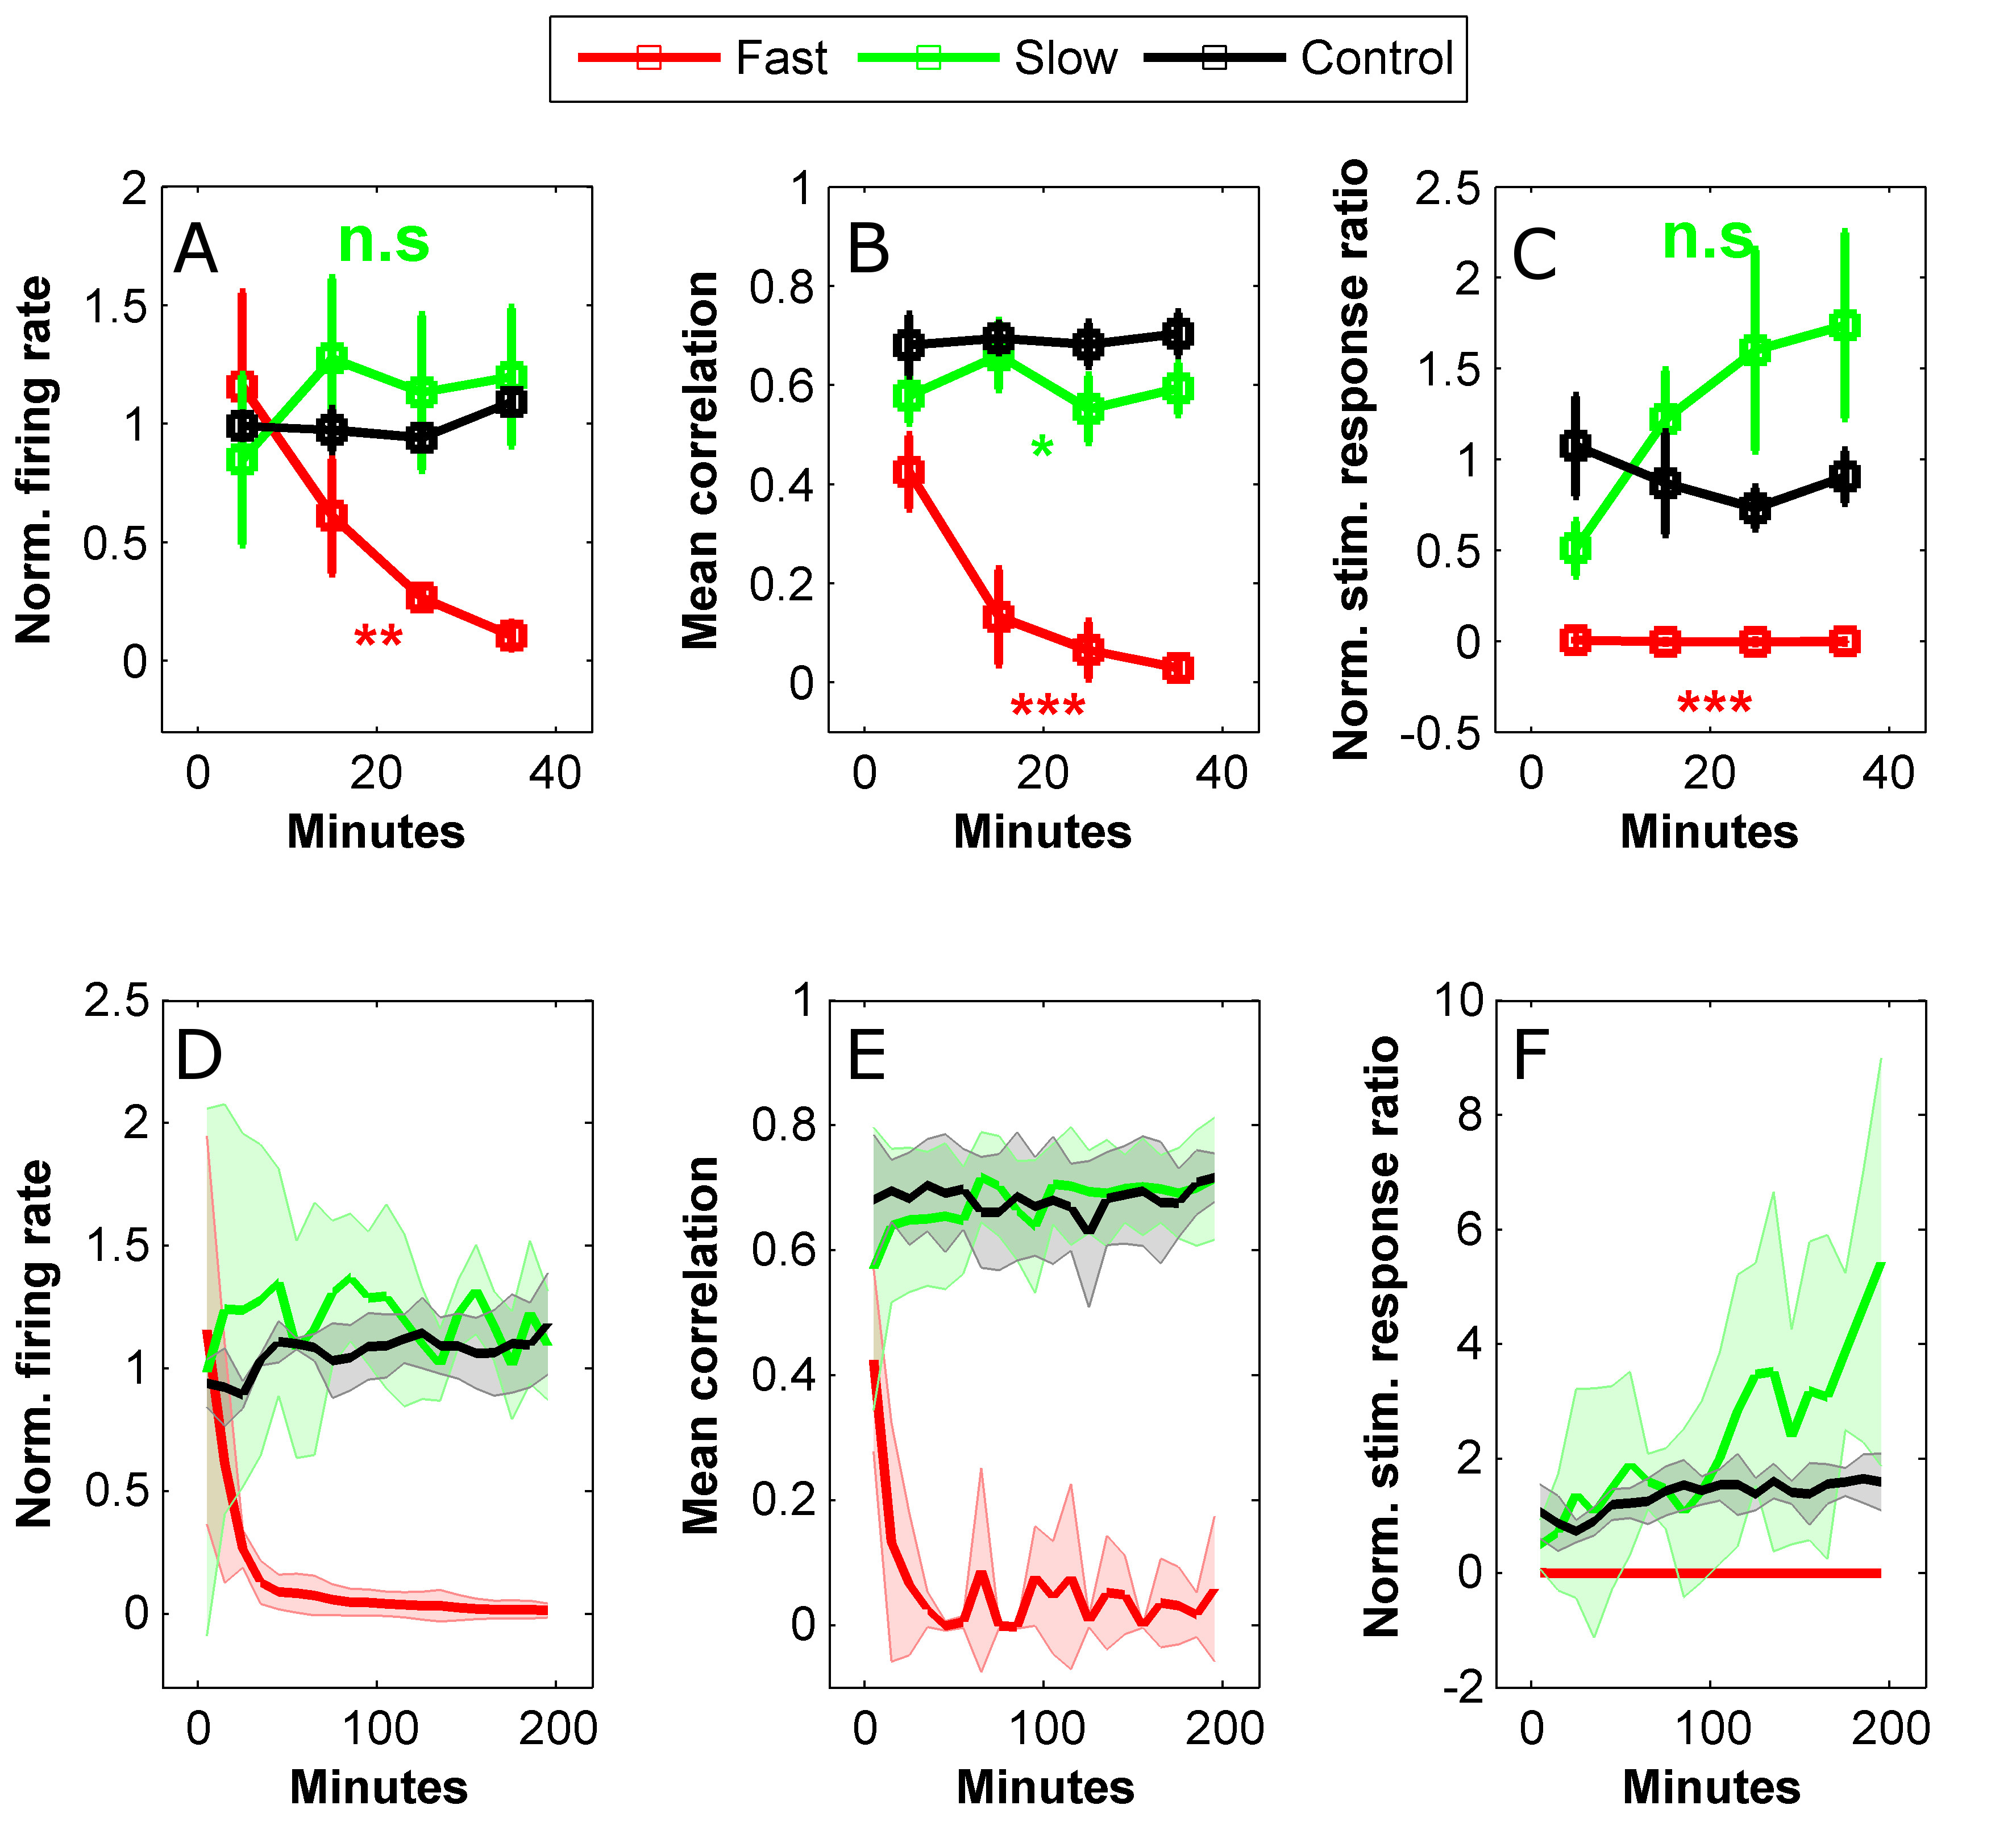
\includegraphics[width=15cm]{chapter5/figures/slowFastStats/slowFastStats.jpg}
            \caption[Averaged time course of activity measures in young cultures placed under flow at different rates]{\textbf{Young cultures placed under flow with self media suffer a flow rate dependent disruption to the activity which does not recover over time.} (A-C) Averaged measures of firing rate, mean correlation and stimulation response ratio in a 40 minute interval immediately after initiation of flow for 2 different flow rates and for recordings in static conditions (color coded). The measures are calculated in 10 minute bins. Error bars indicate SEM. A detailed definition of the measures can be found in the text. Time course of the 3 measures for the 2 flow rates is compared to control by means of a 2-way ANOVA. The statistical significance is determined by the lowest of the p values for group and interaction effects and is indicated by *, **, ***, n.s which refer to confidence levels of 95\%, 99\%, 99.9\% or \textless95\%, respectively. (E-F) Same measures as in A-C in an extended observation period of 200 minutes. All 3 measures crash rapidly with fast, but not slow, flow onset. Shaded area represent the standard deviation of the measures. Firing rate and stimulation response ratio measures are normalized to their averaged value in the baseline recording prior to flow (or to the first hour in the case of the control). Data are based on n=4, 5 and 3 experiments for the fast flow, slow flow and control conditions, respectively.}
            \label{fig:crossFlow:slowFastStats}
        \end{figure}


        \subsection{Using a semi-permeable membrane for shear reduction}
        \label{sec:crossFlow:membrane}
        The results in the previous section reveal a flow rate threshold which cannot be exceeded if the culture is to maintain a stable network activity. Unfortunately, using direct flow at the permissive rate is incompatible with the rapid drug delivery which is the concern of this work and which requires flow speeds in the order of \(1 \frac{mm}{s}\) (see section \ref{sec:devices:protocolDev}). Thus we decided to explore an approach of decoupling the flow from the cells by means of a semi-permeable membrane. In this approach high flow rates would be maintained over the membrane to allow rapid drug delivery to the cell area above the membrane. The next step of the delivery would then be carried out via diffusion. Since the membrane can be positioned in close proximity to the cells this second delivery step can potentially be made as quick as necessary. After all it is known that neurons use diffusion over short distances for inter-cell signalling which can be extremely fast (e.g., synapses). For example, if a \(10 \mu m\) membrane was to be positioned \(5 \mu m\) above the cells giving a total of \(15 \mu m\) drug travel distance then, by using the estimated diffusion time relation \(t\approx \frac{x^2}{4D}\) with \(D=400\frac{\mu m^2}{s}\) (typical diffusion coefficient value for a neurotransmitter sized molecule \cite{johnstoneThesis}), the drug delivery time would be \(\approx 140 ms\) which is easily compatible with the total required agonist pulse time scales. In the case of the devices used here the height of the cell compartment is dictated by the thickness of the tape \(\approx 100\mu m\) so the distance is far greater than that required for rapid delivery. However, the aim here is to test the applicability of the approach and the correct distances can be implemented as needed in drug pulsing devices. Indeed this approach has been implemented before for shear free agonist gradient generation to cultured neurons \cite{morel2012amplification,morel2012concentration}. In that study an analytical estimate was developed for the maximal flow speeds which could be experienced by the cells underneath the membrane as a function of the flow speed over the membrane, of the membrane properties and of the device geometry. Applying this estimate to our devices provides a flow speed of \(20 \frac{nm}{s}\) in the cell compartment at most for the highest possible flow speed over the membrane. This estimate is 2 orders of magnitude lower than even the slow flow rate that was shown to be permissive of proper electrophysiological function in section \ref{sec:crossFlow:slowFast} so this approach holds a potential to sustain the network function.

        \begin{figure}[!htb]
            \centering
            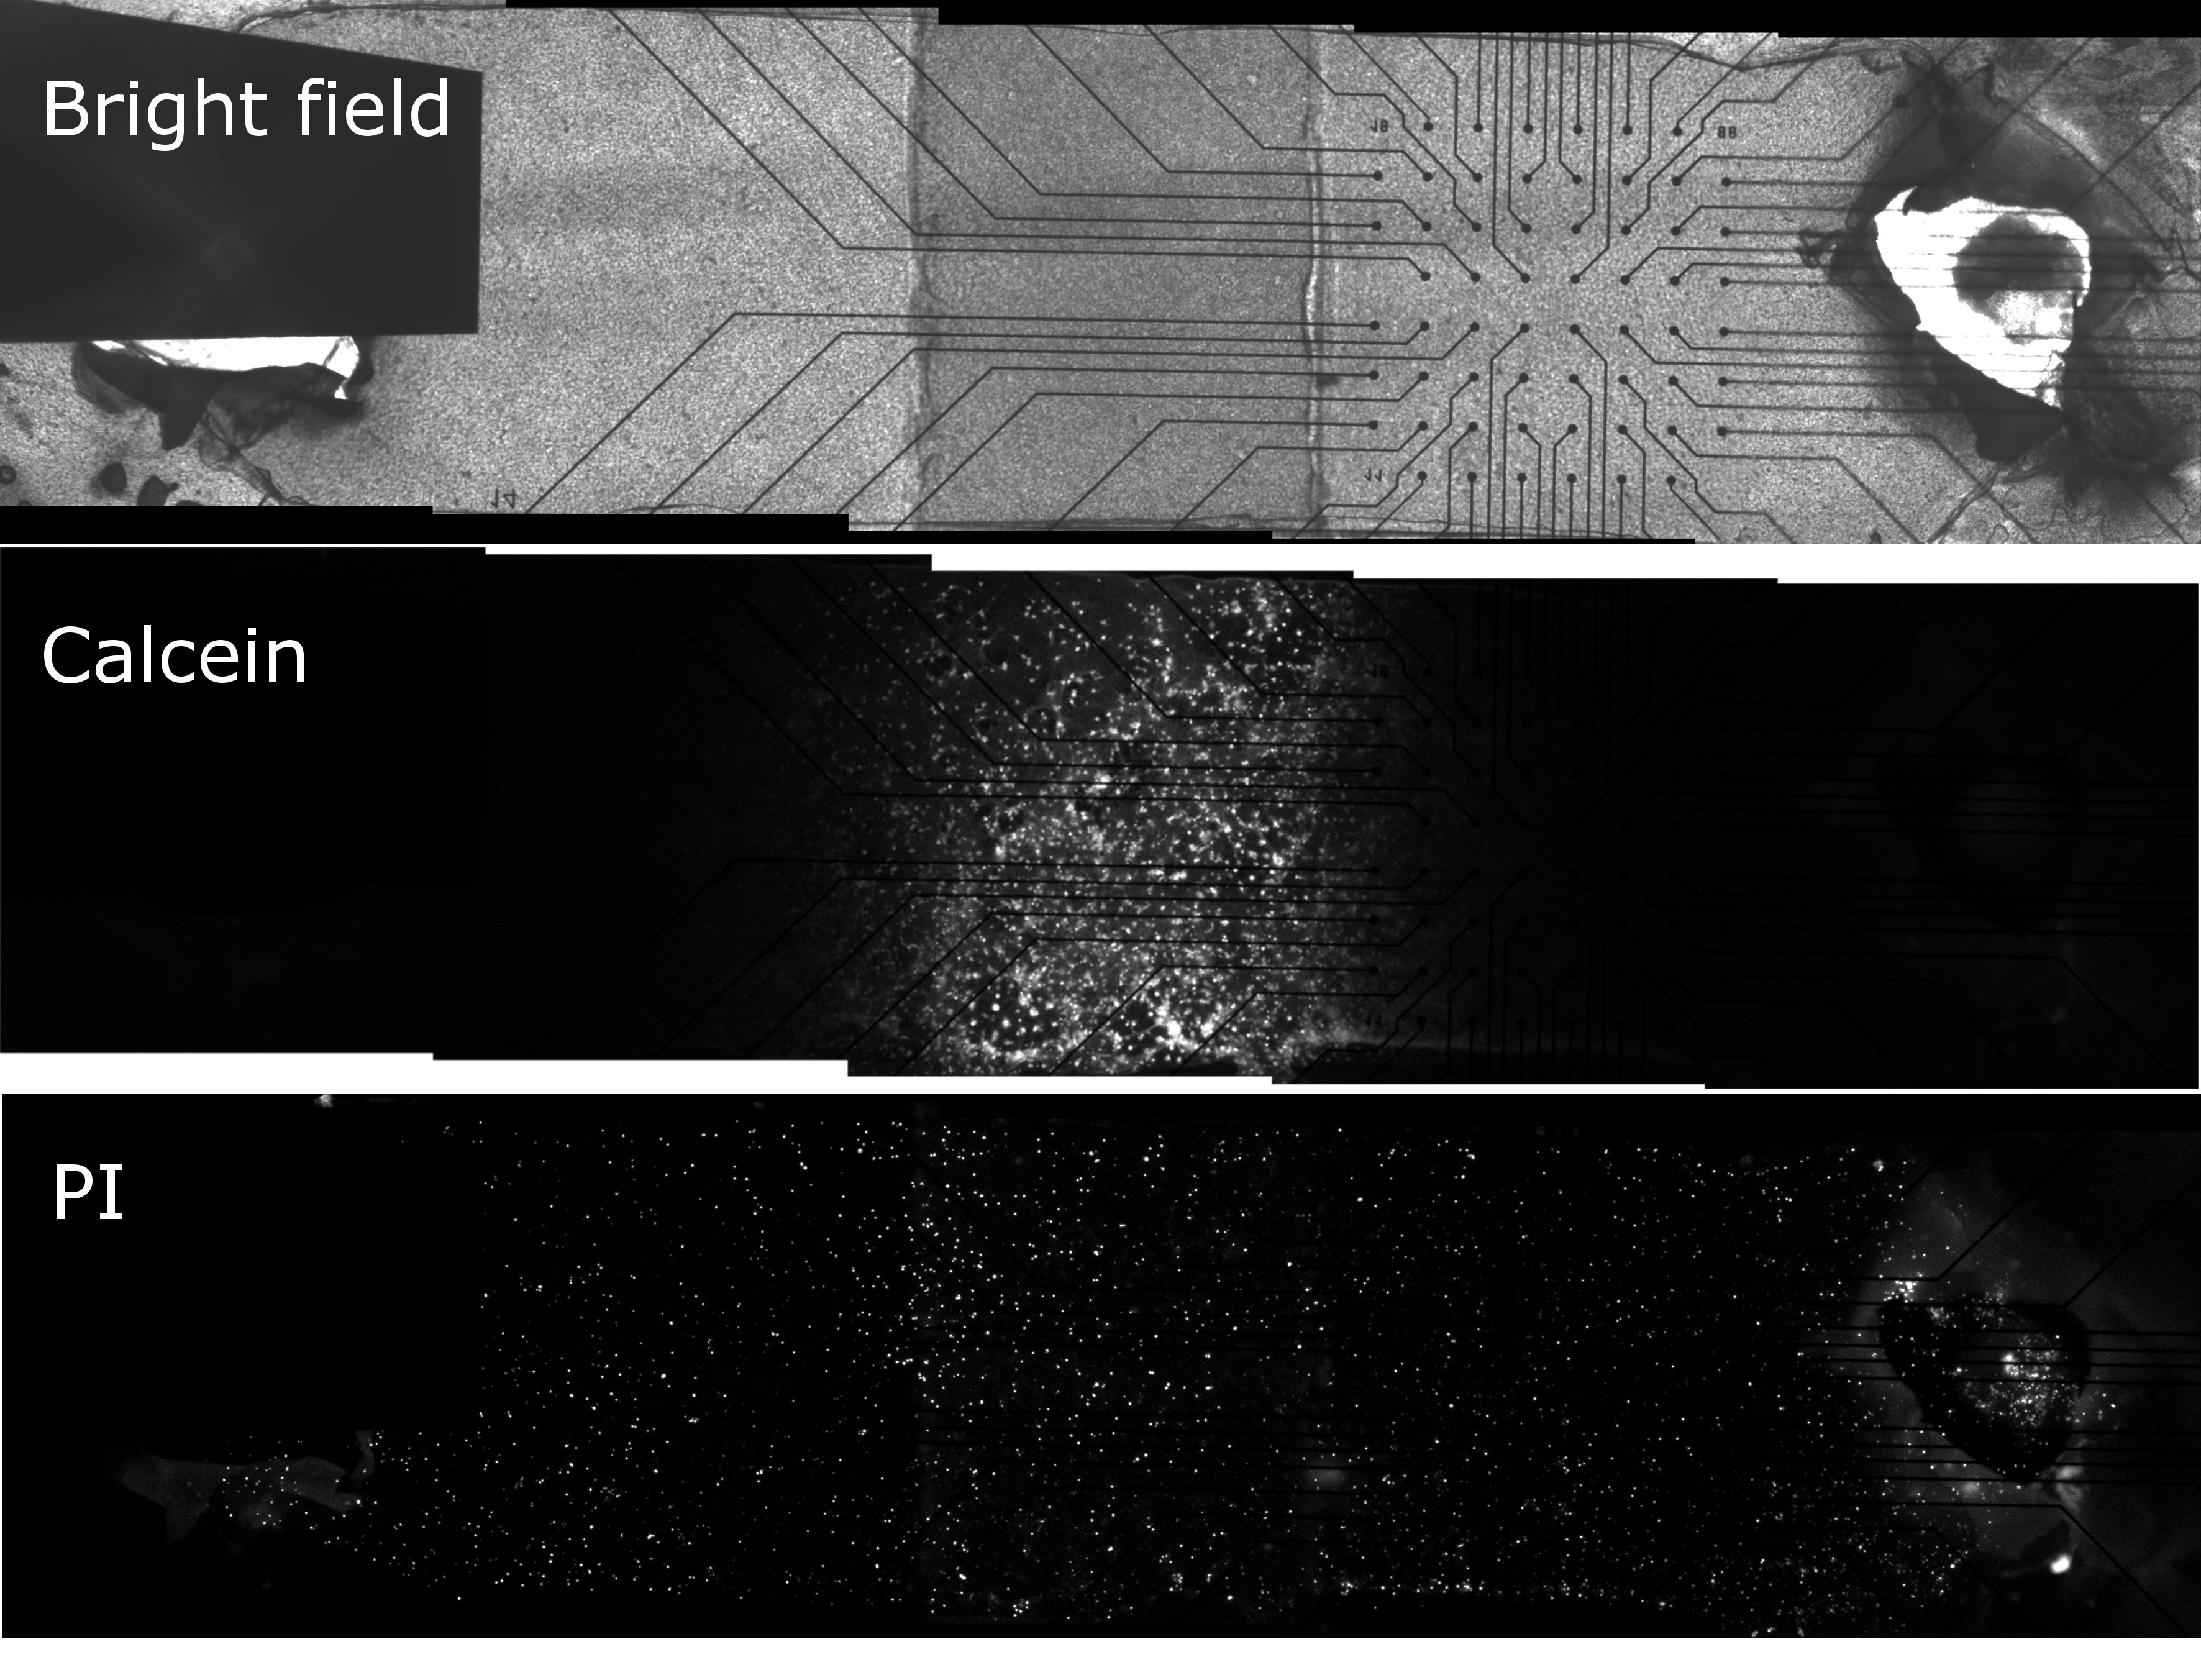
\includegraphics[width=15cm]{chapter5/figures/shiftedMembraneImage/shiftedMembrane.jpg}
            \caption[Bright field and staining images of a culture in a cross flow device inclusive of a semi-permeable membrane]{\textbf{Dead live stained Neuronal culture in a semi-permeable membrane device}. Polycarbonate membrane is not optically clear so cells are hard to distinguish in bright field image. The culture had been under flow with propidium iodide (dead cell stain, see sections \ref{sec:methods:flow} and \ref{sec:devices:viabilityAssay}) for 8 hours so the stain had diffused through the membrane opening to the extents of the culture channel. The live cell stain, Calcein-AM, had been introduced into the flow line only for the final 30 minutes of the flow session so that staining is present only immediately underneath the membrane opening. In this case the recording pads were not positioned directly under the membrane opening but rather shifted to one side.}
            \label{fig:crossFlow:shiftedMembrane}
        \end{figure}

        Young cultures growing in membrane devices were subjected to fast flow under the same protocol as in the previous section (figure \ref{fig:crossFlow:shiftedMembrane} shows images of a culture stained following one such experiment). The results are compared to the fast flow on the non-membrane devices in figure \ref{fig:crossFlow:fastMembraneStats}. Remarkably, the introduction of the membrane did nothing to change the effect of the fast flow on the culture activity with all observed measures crashing with a very similar time course to that of the non membrane devices.

        We also include here the data from a single experiment where the MEA central area which contains the recording pads was not located directly underneath the membrane but was shifted to be entirely inside the non exposed area (figure \ref{fig:crossFlow:shiftedMembrane}). Since this was only a single experiment it cannot be included in a rigorous hypothesis testing analysis so it shown only in the long term plots for impression. This experiment did not include electrical stimulation. The recorded activity and the synchronicity in this case maintained a stable level for the full extent of the flow session. The level of synchronicity was markedly low compared to control but nevertheless stable. These data demonstrate that culture regions which are not placed directly underneath the membrane opening are able to maintain stable electrophysiological function. This experiment provides a positive control for the type of coupling that the culture can have with a flow environment while still sustaining its activity.

        \begin{figure}[!htb]
            \centering
            \includegraphics[width=15cm]{chapter5/figures/fastMembraneStats/fastMembraneStats.jpg}
            \caption[Averaged time course of activity measures in young cultures separated from the fast flow by means of a semi-permeable membrane]{\textbf{Introduction of a semi permeable membrane to decouple the cells from the flow does not improve the activity disruption under fast flow.} Measures are as in figure \ref{fig:crossFlow:slowFastStats} which also contains further information about the data presentation. Note the flow over the membrane (i.e., with \(\approx 100\mu m\) distance imposed between the flow interface and the culture) generates exactly the same effect as direct flow. Data are based on n=4, 3, 3, 1 experiments for conditions of fast flow, fast flow with membrane, control and membrane with shifted recording, respectively.}
            \label{fig:crossFlow:fastMembraneStats}
        \end{figure}

        \subsection{Considerations of diffusive flux}
        The above showed that despite the presence of the membrane the disturbance to the network activity remained as it was before. At first glance, this is surprising because one would expect that the decrease in convective flux due to the presence of the membrane would assist both in diminishing the shear stress and in maintaining a stable chemical environment under the membrane. Thus it could be expected that regardless of the cause of the disturbance, shear stress or convective flux, the membrane should afford protection. However, this intuition does not take into account the diffusive flux which becomes dominant for short distances. Thus, in what follows, we compare the diffusive flux present in the case of the membrane experiments to the convective flux induced by the slow flow.

        Considering a certain conditioning factor species which is produced by the culture and normally present at a concentration \(C \frac{moles}{\mu l}\). Then in the case of direct flow through the channel this species would be carried away by the flow and removed at a flux:

        \[J_{conv}=QC=1\times 10^{-3}C \frac{moles}{s},\] where \(Q=1\times 10^{-3}\frac{\mu L}{s}\) is the volumetric flow rate for the slow flow.

        In the case of the membrane experiments, we assume that the aforementioned conditioning species is not present in the flow media so its concentration above the membrane is \(0\frac{moles}{\mu l}\). We further assume a linear concentration gradient for the species between the cells and the top of the membrane. Then, according to Fick's law the diffusive flux density between the membrane from the cells across the gap and through the membrane is: \[j_{diff}=D\cdot\frac{C}{h}=4\times 10^{-3}C \frac{moles}{s\cdot mm^{2}},\] where \(D=4\times 10^{-4}\frac{mm^2}{s}\) is the diffusion coefficient for neurotransmitter sized molecules and \(h=0.1 mm\) is the height of the cell compartments. To get the total flux through the membrane we multiply the flux density by the area of the membrane opening \(A=4 mm^{2}\): \[J_{diff}=j_{diff}\cdot A=1.6\times 10^{-2}C\frac{moles}{s}.\] Thus the total diffusive flux of the considered conditioning species through the membrane is actually more than an order of magnitude \textbf{higher} than its convective flux during the slow flow experiments. It should be noted that the above calculations include only diffusive flux for the membrane scenario and therefore subliminally assume that the membrane is an ideal diffusive barrier. However, in the case of a real membrane (which is never ideal) the removal flux would be yet more extreme. Another heuristic which emerges from these calculations is that the diffusive flux is inversely proportional to the height of the cell compartment (i.e., the distance between the neurons and chemical sink). In order to equalize the factor removal flux to that of slow flow scenario the membrane needs to be located about \(1-1.5 mm\) away from the cells. This would explain why standard perfusion systems, which exchange media only from the top surface of the culture bath do not exhibit issues with the network activity as seen here. This heuristic fits well with the results from the experiment where the recorded portion of the culture was shifted relative to the membrane opening. In that experiment the recorded cells were positioned at distances between \(400-2000\mu m\) from the membrane which means they were only partially in the `safe' region. Indeed the stable synchronized network activity in that experiment persisted but the effect of the flow was still evident through a decrease in synchronization level compared to the control.

        The diffusive flux considerations discussed here give rise to an important principle: drug delivery through a diffusive barrier designed to introduce a certain agonist at a given rate would inevitably remove molecules of a similar size at the same rate unless they are also present in the delivery media. The results of the membrane experiments, therefore strongly suggest that the self media used for flow does not fully reflect the chemical environment in the internal volume of the devices, even though it was extracted from the same culture dish. In the next section we provide evidence that, in the case of older cultures, this discrepancy is reduced thus providing means to achieve stable activity under rapid flow.

\section{Activity under flow for 3 weeks old cultures}
\label{sec:crossFlow:oldSelf}
        In this section we describe a set of experiments measuring the activity of cultures aged 20-23 days \textit{in vitro} (3 weeks) placed under fast flow with various media formulations. Section \ref{sec:crossFlow:slowFast} described how, when 2 weeks old cultures were placed under fast flow with self media, the network activity was immediately abolished. Remarkably, when an identical experiment was performed on older cultures, the synchronized network dynamics generally persisted under flow, namely with the spontaneous activity proceeding in the form of synchronized bursts, with high values in the correlation matrix and with stable responses to stimulation (figure \ref{fig:crossFlow:youngOldExampleRaster}). Nevertheless, the initiation of flow was associated with an obvious change to the dynamics of the network. In the example shown here, the burst rate seemed to increase (A, right panel) and the stimulation responses became consistently longer (B, right panel). At the same time, the correlation matrix was nearly unchanged (compare C middle and right panels). Further examples are provided in figure \ref{fig:crossFlow:oldOnYoungExampleRaster} which, for example, provide a case where no excitability change was observed but some channels exhibited tonic discharges in discord with the bursts (A, left panel). Thus, in the case of 3 weeks old cultures, the initiation of flow was manifested in a variety of ways but the basic network activity was maintained.

        \begin{figure}[!htb]
            \centering
            \includegraphics[width=15cm]{chapter5/figures/youngOldExample/youngOldRasterExample.jpg}
            \caption[Example for the effect of culture age on the network activity under flow]{\textbf{3 weeks old cultures under fast flow maintain a stable network activity.} Data presented as in figure \ref{fig:crossFlow:slowFastExample} only in this case two different cultures (2 weeks and 3 weeks old) are compared rather than flow rates on the same culture. In this case the activity and stimulation responses are maintained under fast flow with only small modulations. The correlation matrix for static conditions shows the data from the 3 weeks old culture before it was subjected to flow.}
            \label{fig:crossFlow:youngOldExampleRaster}
        \end{figure}

        The stability of activity under flow was consistent over several 3 weeks old cultures from several platings as is shown in figure \ref{fig:crossFlow:youngOldStats} which compares the 3 activity measures introduced in the previous section for young and old cultures under flow as well as for control (static) cultures of the same age groups. The firing rate and synchronicity measures for old cultures are indistinguishable from their controls (2-way ANOVA, \(p=0.084\) and \(0.35\), respectively. P-values given are the minimum between the group and interaction effects). The reported intensification / lengthening of the stimulation response was manifested as a significant two-fold increase in the stimulation response ratio as compared to controls (2-way ANOVA, \(p=2.7\times 10^{-5}\)) but the response was stable throughout the observation period.

        \begin{figure}[!htb]
            \centering
            \includegraphics[width=15cm]{chapter5/figures/youngOldStats/youngOldGraphs.jpg}
            \caption[Averaged time course of activity measures in young versus old cultures under flow]{\textbf{3 weeks Old cultures under fast flow maintain a stable network activity for an extended period of time.} Measures are as in figure \ref{fig:crossFlow:slowFastStats} which also contains further information about the data presentation. Data are based on n=4, 4, 3, 5 experiments for conditions of fast flow on 2 weeks old cultures, fast flow on 3 weeks old cultures, control 2 weeks old cultures and control 3 weeks old cultures, respectively.}
            \label{fig:crossFlow:youngOldStats}
        \end{figure}

        \subsection{The effect of the media source}
        \label{sec:crossFlow:mismatch}
        From collecting the data of the two age groups above, it became clear that, regardless of flow, 2 weeks old and 3 weeks old culture have quite a different underlying connectivity structure. This was manifested, for example, in the response to stimulation where, even though both age groups exhibited responses that were variable in intensity and length, the responses in older cultures always had a low latency component that was very consistent (compare figure \ref{fig:crossFlow:youngOldExampleRaster} B left and right panels at negative times). Furthermore, the differences between the two age groups are further highlighted in figure \ref{fig:app:youngOldCompare} which shows the activity measures in the control experiments (no flow) above in their non-normalized form. This figure shows that the stimulation responses in the 3 weeks old cultures are actually twice as strong and that their synchronicity is higher compared to the 2 weeks old ones. Additionally, all three activity measures are less variable in the older cultures. As mentioned in section \ref{sec:activity:activityStats}, although synapse density peaks at the end of the 2\textsuperscript{nd} week \textit{in vitro} \cite{li2003some}, there is evidence that other synapse related processes such as pruning and changes to the GABA system still significantly affect the network dynamics at later stages (3\textsuperscript{rd} and 4\textsuperscript{th} weeks). The observed increase in the reliability of reverberative response to stimulation might be another manifestation of these later maturation processes although their exact nature is not completely understood. In the present context, it is possible that these age-related changes to the network structure render it more robust to environmental perturbations and therefore could explain why activity is maintained under flow with only minor perturbations. Another age related process which may have to do with the results is ECM formation. It is known that the ECM content in neuronal culture increases over the the 3\textsuperscript{rd} and 4\textsuperscript{th} weeks and that its presence facilitates synaptic function by preventing spill over \cite{bikbaev2015brain}. It is possible  that increased ECM content in the old cultures serves as a protective barrier which allows them to sustain the network activity under flow. The results of the membrane experiments in section \ref{sec:crossFlow:membrane} suggested that the self media lacks important conditioning factors which consequently get removed by the flow causing the activity disruption. It therefore possible that the developed ECM helps to sustain a localized chemical environment by tethering important conditioning factors even if they are not present in the flow media. It is also possible that the more developed synapse formation renders the activity more stable and makes the culture insensitive to perturbation in the environment chemistry. We wanted to test if indeed old cultures are characterized by a reduced sensitivity to the culture media as this information could inform future flow applications. We therefore conducted two more sets of flow experiments. In the first one we used media from young cultures for flow. In the second one we used self media again but performed the experiments 1-3 days following a media change whereby a third of the culture's media was replaced with fresh media (the previous self media experiments in section \ref{sec:crossFlow:oldSelf} were performed 6-9 days following a media change).

        \begin{figure}[!htb]
            \centering
            \includegraphics[width=15cm]{chapter5/figures/mediaChangeStats/mediaEffectStats.jpg}
            \caption[Averaged time course of activity measures in old cultures under flow with different media types]{\textbf{The type of media used for flow strongly modulates the activity of the cultures and can cause the activity to crash.} Measures are as in figure \ref{fig:crossFlow:slowFastStats} which also contains further information about the data presentation. Data are based on n=4, 4, 4, 5 experiments for self media, 2 weeks old media, changed 3 weeks old media and control respectively.}

            \label{fig:crossFlow:mediaChangeStats}

        \end{figure}

        Figure \ref{fig:crossFlow:mediaChangeStats} shows the results of flow with the two media types described above. Interestingly, flow with media taken from 2 weeks old cultures (blue curves) resulted in a dramatic disruption to the activity of a similar nature to the one previously observed in the younger cultures under self media, namely that all 3 measures immediately destabilized. However, there were also some obvious differences: Firstly, the total firing rate initially jumped 4-fold and despite dipping rapidly it stayed elevated compared to the control for the first 40 minutes (2-way ANOVA, \(p=5.0\times 10^{-5}\)). In fact, the firing rate decreased to a level lower than control only after about 100 minutes and was never abolished completely. Secondly, the correlation levels were significantly reduced as compared to control immediately with flow onset (2-way ANOVA, \(p=1.0\times 10^{-12}\)) but deteriorated more gradually compared to the 2 weeks old cultures (compare to figure \ref{fig:crossFlow:fastMembraneStats}) and were never completely abolished. Finally, the response to stimulation initially persisted (2-way ANOVA on the first 40 minutes did not reveal a significant difference from control, \(p=0.90\) for group effect and \(0.28\) for interaction effect). However, after 40 minutes the response was already significantly below control (unbalanced t-test on the final sample of panel C, \(p=0.0038\)) and crashed to 0 soon after. Thus these results demonstrate that older cultures are somewhat more robust to the chemical perturbation induced by the flow. However, the overall trend of their activity measures under flow is remarkably similar to those of younger cultures under flow with the same media type (compare figure \ref{fig:crossFlow:mediaChangeStats} blue curves and figure \ref{fig:crossFlow:youngOldStats} red solid curves) therefore implying a dominant role for media chemistry in maintaining the network dynamics regardless of age.

        The high degree of sensitivity of 3 week old cultures to the chemistry of the flow media is further demonstrated by the fact that the mere action of changing the media prior to its use as self-media can significantly affect the the culture's dynamics under flow (red curves). In a 40 minute window after flow initiation this was mainly evident in increase in firing rate as compared to control (2-way ANOVA, \(p=6.5\times 10^{-6}\)) whereas the synchronicity was reduced only with a 90\% level of confidence (2-way ANOVA \(p=0.054\) for group effect). The stimulation response was significantly stronger than control (\(p=7.3\times 10^{-4}\)) but an increase with the same level of confidence was found for the original flow experiment with self media on old cultures. The long term trends show a less stable behaviour under flow with recently changed media in all 3 measures. Nevertheless, the effects of the media change were subtle compared to flowing with 2 weeks old media and we considered this case as useful for experimentation.

        To summarize, The results provided in this section demonstrate a high sensitivity of 3 weeks old cultures to the source of the flow media, to the extent that they cannot maintain stable network activity in much the same way that the 2 weeks could not under flow with the same type of media. This demonstrates that the stable activity observed in the older cultures with self media was predominantly in virtue of the saturation of the bulk media around the cells (which is used as the self media) with age-dependent conditioning factors.

        \subsection{How 3 weeks old conditioned media performs on 2 weeks old cultures}
        \label{sec:crossFlow:oldOnYoung}
        The results of the previous section suggest that media drawn from 3 weeks old cultures contains chemical species that enable stable network function under flow and that these species are absent in media from younger cultures. This led us to ask whether these enabling features of 3 weeks old media are specifically linked to older cultures or are they more universal and would facilitate stable network function under flow for younger cultures as well. To answer this question, we conducted a final set of experiments where media taken from 3 weeks old cultures was used for flow on 2 weeks old ones. Figure \ref{fig:crossFlow:oldOnYoungStats} shows the results of these studies using the same measures used before. Interestingly, old media did in fact improve the performance of younger cultures. These cultures generally did not exhibit the desynchronized tonic firing that previously characterized the activity in this age group under flow. Even though the activity measures decayed within the observation period, they were initially stable and the deterioration was much slower than with self media (figure \ref{fig:crossFlow:oldOnYoungStats}). Nevertheless, a striking difference that was manifested in these younger cultures as compared to their older counterparts was that the firing rates and the stimulation responses were immediately depressed upon the onset of flow and so had lower values than control (figure \ref{fig:crossFlow:oldOnYoungStats} A,C 2-way ANOVA, \(p=0.013\) and \(0.016\), respectively, group effect). Synchronicity was also decreased (\(p=0.011\)). This depression is the opposite effect to what was observed with older cultures subjected to flow with the same media type where the stimulation responses were, on average, doubled in intensity. These older cultures also tended to show an increase in the activity when any form of media with reduced conditioning levels was used (media from younger cultures or recently changed self media, previous section).

        \begin{figure}[!htb]
            \centering
            \includegraphics[width=15cm]{chapter5/figures/oldOnYoung/oldOnYoung.jpg}
            \caption[Averaged time course of activity measures in young cultures under flow with old media]{\textbf{3 week old media media partially maintains the activity 2 week old cultures under flow but induces depression.} Measures are as in figure \ref{fig:crossFlow:slowFastStats} which also contains further information about the data presentation. Data are based on n=4, 4, 3 experiments for self media, 3 weeks old media and control respectively.}
            \label{fig:crossFlow:oldOnYoungStats}
        \end{figure}


        Taken together with the results of the previous section, the data shown here indeed suggest that 3 weeks old media, possibly due to the prolonged time in culture, is saturated with conditioning factors which promote stable network activity under flow in cultures in the same age as well as in younger ones. However, this media is more effective when matched with it own age group (i.e., the 3 weeks old cultures). Moreover, the two age groups exhibited contrasting acute effects (i.e., immediately on the onset of flow) when placed under flow with media from the other group (depression versus excitation). These opposite acute effects hint that 3 weeks and 2 weeks old cultures differ in their excitatory or inhibitory tone (possibly in the tonic level of neurotransmitters) and that this tone would needs to be matched by the flow media for optimal results. Examples for these tonic shifts are further presented in figure \ref{fig:crossFlow:toneExampleRaster}. These data indicate that the flow media chemistry needs to match the specific identity and developmental stage of the culture at hand.


        \begin{figure}[!htb]
            \centering
            \includegraphics[width=15cm]{chapter5/figures/toneRasterExample/toneRasterExample.jpg}
            \caption[Examples for the effect of a mismatch between the media age and the culture age]{\textbf{Rapid flow with mismatched media caused an acute switch in the culture's excitatory/inhibitory tone.} The direction of the tonic shift depended on the specific age/media combination. Data presented as in figure \ref{fig:crossFlow:youngOldExampleRaster}.}
            \label{fig:crossFlow:toneExampleRaster}
        \end{figure}


\section{Interpretation of the activity under flow results}
\label{sec:crossFlow:interp}
In the previous chapter we have reported that conditioned media can sustain neuronal viability under flow. However, the nature of interaction between the media and culture and cause of the degeneration remained unclear. In this chapter, we extended the flow experiments to observe the network action potential activity under flow and gained valuable insight as to how flow bears on the culture tissue. Previous flow microfluidic work focused on the need of mitigating shear \cite{morel2012amplification,wang2008microfluidics} which neuronal tissue is exposed to and attributed the positive effects of the chemistry of the flow media on the viability to `shear protection' by molecules secreted specifically for that purpose \cite{liu2013galanin}. In this work we observed a strong disruption to the network activity under fast flow. Indeed this could be attributed to shear activating stretch receptors or simply tearing up the cellular membranes and eliciting an inflammatory response. However, using a semi-permeable membrane shown to reduce the shear to negligible levels \cite{morel2012concentration} did not result in any improvement whatsoever. Furthermore, the membrane results were consistent with an assumption that a neuromodulator sized chemical species (\(D=400\frac{\mu m^{2}}{s}\) \cite{johnstoneThesis}) is being diffusively removed through the membrane opening. Calculation based on this scenario predicted that cells located at a distance of \(1-1.5 mm\) from the diffusive sink would be `safe' from the removal. Indeed the shifted recording experiment showed that a culture area partially located in the safe distance maintained its activity with only minor modulation. Had we performed the calculations with diffusive coefficients of ions (\(D=4000\frac{\mu m^{2}}{s}\)) or small proteins  (\(D=40\frac{\mu m^{2}}{s}\)) then we would have expected either a disruption to occur over the entire culture area of the device or no disruption at all, respectively. However, these predictions are in disagreement with the results thus pointing specifically to neurotransmitter sized molecules as the culprits. This notion is strongly supported by the observation that flow with mismatched media (i.e., media extracted from culture dishes of a different age group) causes a strong tonic shift in the excitability of the cultures depending on their age. Thus, we are able to aasert, with high degree of confidence, that the immediate activity effects observed here are best explained by action of neurotransmitters on their respective receptor ion channels and that other explanations involving shear should be rejected on the basis of an Occam's Razor reasoning. The results shown in this chapter do not rule out the possibility that shear contributes to other long term effects but they definitely demonstrate a that a disruption to neuronal signalling is a strong part of the effect of flow which  needs to be taken into account.

In section \ref{sec:crossFlow:oldSelf} we showed that the activity in 3 weeks old cultures was maintained under fast flow with self media but this was not the case for 2 weeks old cultures with their own self media. This discrepancy is not just a result of age dependent differences in network structure or ECM levels because the media from the older cultures actually maintained the activity of the younger ones better than their own (section \ref{sec:crossFlow:oldOnYoung}). This result suggests that self media in old cultures is chemically more matched with the micro-environment around the cells than in younger cultures . Nevertheless, as the self media is in direct contact with the culture one would expect chemicals secreted by the cells to quickly diffuse to the bulk, especially in the case of small neurotransmitter molecules, so it may seem surprising that a strong gradient would develop between them. However, as mentioned in sections \ref{sec:introduction:MEANetwork} and \ref{sec:activity:activityStats}, the period of development occurring between the young (beginning of 3\textsuperscript{rd} week) and old age (beginning of 4\textsuperscript{th} week) time frames is characterized by significant changes to the neurotransmission systems. HPLC measurements of the glutamate and GABA contents of neuronal culture media show that the levels of both these major neurotransmitters rise over the first month \textit{in vitro} and saturate only at around day 35 \cite{ramakers1994activity}. In particular, the GABA levels do not rise monotonically but remain low for the first 3 weeks and then jump sharply to reach the final saturated levels. This rise in the media GABA content might correlate with the induction of the astrocytic GABA release \cite{lee2010channel} or maturation of late interneurons \cite{hensch2005critical}. Additionally, some reports claim that synaptogenesis in culture extends into the forth week which might also explain the increase in neurotransmitter production during the preceding period \cite{brewer2008neuron,grabrucker2009synaptogenesis}. Although the exact nature and timing of these maturation processes has not been completely clarified, there is ample evidence that the tonic neurotransmitter levels strongly depend on the culture age. In our devices, a large support culture comprising 250k cells is seeded on the outside (compared to 14k inside) and this external culture is probably the main source for diffusible factors in the bulk media. A possible explanation for the mismatch of the self media in 2 weeks old cultures could therefore be that the external support cultures were at a considerably different developmental stage as compared to the internal cultures and so the self media was not well matched to the latter. Indeed it has been shown that cultures grown in microfluidic devices develop faster than standard ones, possibly due to localized buildup of conditioning factors \cite{goyal2011neuronal}. older devices, which are one week more developed, both the internal and external cultures may have entered a saturation in development so they were more similar. Another possible explanation for the self media mismatch is that during periods of accelerated development the rate of changes to the local neurotransmitter environment exceeds the rate of diffusion so that the bulk media is `lagging behind' in accumulating the chemicals from the microenvironment. After all, even though neurotransmitters are small molecules they would take about 17 hours to diffuse through a media reservoir of height \(10 mm\) (note that the bulk media volume per sample was bigger in the cross flow devices to allow enough supply for the flow session).

The afore-mentioned delay in development of some GABAergic elements of the neurotransmission system raises the possibility that it is indeed GABA that is lacking in the flow media. Indeed it has been shown that the action of tonic extrasynaptic GABA exerts inhibition that is several times \textbf{stronger} than that of the fast synaptic one \cite{farrant2005variations,mody2004diversity} which could explain how drastic the effects of flow are. This notion aligns well with the immediate tonic shifts observed under flow with media from a mismatched age group (figure \ref{fig:crossFlow:toneExampleRaster} and sections \ref{sec:crossFlow:mismatch} and \ref{sec:crossFlow:oldOnYoung}). Namely, when 2 weeks old media was used on 2 weeks old cultures the response was an immediate 4 fold increase in the spiking activity followed by a gradual decay, possibly due to depletion of resources. This could be interpreted as a release from strong inhibition. On the other hand, when the opposite combination was used the activity and stimulation response were immediately halved. This could be explained by the young cultures being accustomed to lower levels of tonic inhibitor compared to the old cultures and hence becoming silent when exposed to media from the latter. Indeed GABA is recognized as the major inhibitory neurotransmitter operating in the CNS and its extrasynaptic function has been receiving growing interest \cite{mody2004diversity,lee2010channel,olah2009regulation}. Nevertheless, the activity patterns observed under fast flow with young conditioned media are inconsistent with results from application of GABA antagonists \cite{bikbaev2015brain,li2007long}. These studies did not report a decrease in synchronization but rather an increase in burst frequency and burst length so removal of GABA alone is probably not enough to explain the observed disturbance. Intrinsic volume transmission comprises an assortment of other signals including the major excitatory neurotransmitter glutamate \cite{cavelier2005tonic} as well as adenosine \cite{wall2015localized}, ATP, NO and various neuropeptides \cite{fuxe2010discovery,taber2014volume}. Thus the observed disturbance cannot be attributed to any specific species and is more likely a holistic effect associated with perturbations to all the intrinsic volume transmission processes at varying degrees. We believe that our results warrant an in depth investigation into the source of the disruption as it could entail a novel signalling species. Such an investigation could proceed by applying a cocktail of receptor blockers matching the known volume transmission signals to see if the effects of flow may be reproduced in this manner.

Even when the media is matched the flow could still affect more than just the extrasynaptic tonic concentrations of signalling molecules. This is explained next.  The accepted paradigm is that neurotransmission proceeds in two distinct compartments, intra- and extra-synaptic. The most recognized neurotransmission action is the fast synaptic one where vesicle release on the presynaptic side causes an extremely rapid (time constant \(<1ms\)) phasic increase in the neurotransmitter content in the synaptic cleft. The time course of these phasic signals is mainly determined by outwards diffusion to the extrasynaptic space \cite{clements1996transmitter}. Although the phasic dynamics are the hallmark of synaptic function it has also been established that there is an appreciable tonic concentration of neurotransmitters in the synaptic cleft which is enough for a continuous activation of postsynaptic receptors \cite{sah1989tonic}. The source of this tonic transmitter level is most probably simply diffusion from the extrasynaptic space. In contrast to the intrasynaptic compartment where only neurotransmitters are known to operate, the extrasynaptic compartment contains a mixture of neurotransmitters and neuromodulators operating through both ionotropic and metabotropic receptors. In recent years, more focus has been given to the extrasynaptic species which were shown to have a strong effect on network dynamics and therefore a computational importance \cite{wall2015localized,mann2010control,hamann2002tonic,lenk2016understanding,cavelier2005tonic}. Such extrasynaptic neurotransmitters and neuromodulators are usually referred to as the 'tonic environment'. However, this terminology could be misleading by giving the impression that this environment is completely static whereas in fact it is temporally varying (i.e., it has phasic aspects) or else it would not be able to modulate the network activity. Since this intrinsic volume transmission is based on discrete secretion events from specific cells it stands to reason that it will have a spatial organization as well (this was shown for the case of adenosine in \cite{wall2015localized}). Thus, to summarize, both intra- and extra-synaptic compartments contain signals with tonic and phasic components and they are not completely segregated but rather coupled via diffusion (e.g., synaptic spill over contributes to the phasic extrasynaptic signals and changes to extrasynaptic concentrations of non-synaptic origins can influence the tonic activation of the synapses).

\begin{wrapfigure}{r}{5cm}
      \centering
      \includegraphics[width=5cm]{chapter5/figures/synapse/synapseIllustration.jpg}
      \caption[Illustration of a synaptic cleft with flow running through it]{Illustration of the synaptic cleft geometry and symbols used to compare the convective and diffusive flux in the case where the flow runs directly through the synapse.}
      \label{fig:crossFlow:synapse}
\end{wrapfigure}

Out of the signalling modes mentioned above, The phasic synaptic one is the least likely to be affected by the flow because the neurotransmitter pulses are extremely quick and the concentrations are dependent on release from vesicles which are located intracellularly. Nevertheless there is a concern that if rapid convective flow is channeled through the synaptic cleft then it could wash away the neurotransmitter molecules as they are released and therefore to significantly modify the temporal profile of activation. To check if this could indeed be of concern we compared the diffusive flux out of a synapse with the expected convective flux due to flow assuming that the synapse is indeed open and that the flow is directed perpendicularly to the transmission line as depicted in figure \ref{fig:crossFlow:synapse}. The calculations are as follows: assuming a parabolic flow profile the flow velocity around the synapses is \[u=u_{avg}(1-\frac{y^{2}}{h^{2}})\approx 15\frac{\mu m}{s}\] where \(u_{avg}=200\frac{\mu m}{s}\) is the average flow velocity, \(h=50\mu m\) is half the channel height and \(y=48\mu m\) is the location of the synapses relative to the horizontal center of the channel, i.e., \(2\mu m\) from the surface. The diffusive flux out of the synapse is \[J_{diff}=D\frac{c-b}{d}(4A)\approx 32(c-b)\frac{moles}{s}\] where \(D=400\frac{\mu m^{2}}{s}\) is the diffusion coefficient for a neurotransmitter sized molecule in free media, \(c\) and \(b\) are the intra- and extra-synaptic neurotransmitter concentrations, respectively in \(\frac{moles}{\mu m^{3}}\), \(d=0.2\mu m\) is the diffusion distance and \(A=0.2\times 0.02=0.004\mu m^{2}\) is the area of one external face of the synaptic cleft (taking the cleft gap to be \(0.02\mu m\) and cleft width to be \(0.2\mu m\)) (\(4A\) is then the entire face area available for diffusion). The total convective flux is \[J_{conv}=J_{flowout}-J_{flowin}=Auc-Aub=Au(c-b)=0.06(c-b)\frac{moles}{s}.\] Thus, somewhat un-intuitively and owing to its nano-scale dimensions, the outwards flux out of the cleft due to diffusion (which is the main determinant of the temporal concentration profile during synaptic activation \cite{clements1996transmitter}) is 3 orders of magnitude larger than the that due to convection even if the cleft is completely open to the flow. In reality, the synapses are usually enveloped in neuronal and astrocytic membranes which are unlikely to allow any degree of flow through. Thus we would expect phasic synaptic dynamics to be maintained even under much faster flow rates or shallow device geometries (i.e., where the flow velocity at the boundaries would be higher). However, the same cannot be said about the phasic extrasynaptic signalling which is much slower and operates over much larger space scales and about tonic synaptic concentrations. Thus, fast flow, beyond the obvious effect of changing the basal extrasynaptic species concentrations, could have generated the observed disruptions by indirectly changing the tonic receptor activation within the synapses and also by disturbing the phasic (and spatially organized) aspects of the intrinsic volume transmission.




\section{Chapter conclusion}
We initiated the investigations performed in this chapter by admittedly making a technical leap whereby we switched to using `self media' rather than the conditioned media protocol introduced for the viability experiments in the previous chapter (section \ref{sec:devices:viabilityAssay}). Although the idea to use self media came about by chance exploration in the lab, we hope that the results and interpretation presented in this chapter have made it clear why this media formulation is the best approach for achieving stable network function under flow. The paradigm employed in the case of the viability experiments assumed that neurons are singular entities that would always respond in the same way to a particular level of treatment (e.g., to a value of the conditioning scale). This may be partially true where viability is concerned but in the case of network activity we found that age is a crucial parameter that determines how the culture would respond to a particular media formulation. More specifically, the flow media needs to be matched to the specific developmental stage of the culture and this simply prescribes using the bulk media from the same culture dish, i.e., self media. At present, it is not clear to what extent these principles apply also to viability. Viability is mostly associated with a family of signalling processes distinct from those playing a role in the activity such as secretions of growth factors or even of ECM proteins. However, these such trophic processes might also have an age dependent nature. Additionally, the results in this chapter showed that when mismatched media was used, in some cases the effects on the activity were so severe, that the culture was driven out of its working range and seemed to run out of resources to maintain even basic network function. It is not unreasonable to assume that such cases would also involve indirect effects on the viability. It is worthwhile to note, in this context that all the flow work in chapter \ref{chap:devicesAndFlow} was performed in a parameter space which we now know to be of network disfunction. Thus, these results warrant further investigation into how the media affects both the viability and the activity to see if a protocol can be found that is optimal in both respects.

An additional insight the arises from the data presented in this chapter is that the flow interferes with signalling molecules very close to the cells, i.e., with intrinsic volume transmission processes. In hind sight, it is fairly obvious that a system designed to deliver agonists to cells at fast rates would also remove resident molecules equally rapidly. This notion of control over local concentrations of signalling molecules in close proximity to the cells is unique to this system and may actually be useful if utilized properly. We will further develop this idea in chapter \ref{chap:Discussion}.

Lastly and most importantly we have identified conditioned where the network activity is adequately maintained under fast flow (3 weeks old cultures and self media). This flow protocol will be the basis for the final agonist pulsing system described in the next (and final) chapter.


\label{sec:crossflow:conc} 
%\chapter{Rapid programmatic agonist delivery to a neuronal microculture}
\label{chap:microculturePulses}
\section{Introduction}
In this chapter we combine all the components developed in previous chapters to construct a system with the capability of second-scale agonist pulsing over an entire neuronal microculture. To this end, we will start by providing a new design for microwell devices, taking into account the lessons learnt from the pilot design in section \ref{sec:devices:microcultures}, and growing neuronal microcultures in them. Specific further tweaks to the protocol which were needed to achieve satisfactory results will be discussed. Secondly, we will test the device's pulsing performance by visualizing the agonist time course using a fluorescent molecule. We will further showed that the pulsing performance can be accurately predicted using a numerical fluid dynamics simulation in Comsol which will be important for future designing of devices that meet bespoke pulsing requirements. We will further test ability of the devices to generate a biological response at the required time scales was demonstrated via pulsing of glutamate and recording the neuronal activation on microelectrode arrays. Finally, the devices will be used to generate dopamine pulses coupled to electrical stimulations. By running these final experiments we will have effectively realized the Izhikevic thought experiment (section \ref{sec:introduction:izi}) and achieved the declared goal of this Ph.D.

\section{Fabrication and establishment of long term neuronal microcultures}
\label{sec:pulses:microcultures}
The devices were based on a 2-layer design comprising a PDMS microwell layer and a tape-based flow layer. The design is illustrated in figure \ref{fig:pulses:circularIllustration} and the fabrication process is described next. The PDMS layers used in this section were manufactured using thin film spinning (section \ref{sec:methods:fabrication}, either \(120\) or \(80 \mu m\) thick). They were based on the design introduced in section \ref{sec:devices:microcultures} which includes a main experimental microwell together with a large rectangular support well. The distances were selected so that the support well would be placed on top of the internal reference electrode of the MEA to allow it contact with the media. The microwell was created using a \(0.8 mm\) biopsy punch whereas the support well was cut manually using a scalpel. In this manual procedure, the dimensions were adhered to by placing the cured PDMS sheet on top of a printout of the layer design for reference. The earlier pilot study showed that microcultures exhibit a high rate of degeneration, depending on their size, and that the largest microwell sizes used in that study, \(400\times 400 \mu m^{2}\), were able to match the viability of macrocultures. The punched microwells in the new design were of average diameter of \(675 \mu m\) placing them further in the safe zone. The flow layer was cut out of a \(50 \mu m\) silicone transfer tape (section \ref{sec:methods:fabrication}). The assembly process started by joining the flow layer to a pre-cured PDMS bulk and punching of the ports. All elements were then heat sterilized in \(120\degree C\). Next, the microwell layer was placed on top of a commercial MEA pre-coated with PEI (section \ref{sec:methods:surface}) while aligning the microwell and the support well with the central recording and the reference electrode, respectively. A reversible hydrophobic bond is generated when PDMS is put in contact with a glass surface. This was followed by joining of the flow layer (and the PDMS bulk) with the top surface of the microwell layer while making sure that the microwell is positioned as close as possible to the apex of the channel. The device was completed by gluing a glass chamber around the device to hold the growth media (figure \ref{fig:pulses:circularIllustration} bottom images). The devices were seeded by pushing \(2 \mu L\) of seeding suspension at a density of \(12\times 10^{6} \frac{cells}{ml}\). The density was found to play a significant role which will further addressed later. After 1 day of incubation the devices were flushed to remove excess cells from the top of the PDMS sheet. In contrast with how the microcultures were prepared in section \ref{sec:devices:microcultures}, the surface-then-bonding approach used here guaranteed that only the microwell surface was cell adhesive so the cells on top of the PDMS sheet were not strongly attached. This allowed us to use a more delicate flushing routine to avoid any removal of cells from the microwell. This proceeded by using a syringe driver to apply a controlled flow rate of \(50\frac{\mu L}{min}\) for about 20 seconds which was effective at removing the excess cells (figure \ref{fig:pulses:clearanceDemonstration} A-B). The MEAs used in the study were either of the standard 8x8 layout with \(200 \mu m\) inter-electrode spacing or HDMEAs where the electrode pads were closely packed together in 2 blocks of 5x6 configuration at \(30 \mu m\) spacing (see section \ref{sec:methods:MEARecording}). In the first case the microwell was aligned so that 9 electrodes would be contained with in its area. In the second case one block of 30 electrodes could fit into the microwell area. An example for the later case may be seen in figure \ref{fig:pulses:clearanceDemonstration}. 

  \begin{figure}[h]
       \centering
       \includegraphics[width=15cm]{chapter6/figures/circularIllustration/circularIllustration.jpg}
       \caption[Illustration of the new microwell devices used for dopamine pulsing on a microculture]{\textbf{Illustration of the microwell devices.} Illustrations showing the constituent layers of the device laid out as well as assembled and joined to an MEA. The dimensions of the flow and microwell layers are also shown in millimeter units. Also shown are images of the device before and after gluing of glass cylinder to hold the media reservoir. Further details about the device fabrication are found in the text.}
       \label{fig:pulses:circularIllustration}

  \end{figure}

\subsection{PEI-then-all-tape devices}
    In preliminary versions of the device the microwell layer was composed of silicone transfer tape as this was expected to improve the bonding between the layers and reduce leaks. However, despite the good results obtained with devices made purely out of tape in section \ref{sec:devices:bonding}, the microcultures in this case exhibited poor adhesion and did not develop normally (figure \ref{fig:pulses:tapeMicroculture}). In a previous study toxic effects of leaching from PDMS, which is generally considered safe, presented themselves in microfluidic devices of extremely small geometries \cite{millet2007microfluidic}, presumably because of an increased leaching surface to media volume ratio. We reasoned that a similar issue arises in our devices but with tape being the source of the leaching so we switched to extracted PDMS (section \ref{sec:methods:fabrication}) for production of the microwell layer. Indeed this modification succeeded in providing the right conditions for microculture growth, as shown next.

  \begin{figure}[h]
       \centering
       \includegraphics[width=15cm]{chapter6/figures/tapeMicroculture/tapeMicroculture.jpg}
       \caption[Microcultures grown in all-tape devices exhibit bad surface adhesion]{\textbf{Devices made purely out of silicone transfer tape are unsuitable for neuronal adhesion.} Images of a culture seeded into devices where both flow and microwell layers were made out of silicone transfer tape (\(50\) and \(125 \mu m\) thick, respectively). The cells aggregated immediately after plating and formed a single cluster after a few days. Scale bar is \(200 \mu m\) long and is consistent across both images.}
       \label{fig:pulses:tapeMicroculture}
  \end{figure}

    \subsection{PEI-then-PDMS-tape device}
    Microcultures generally grew well in the PDMS / tape chimera devices and were usually viable into the 4\textsuperscript{th} week \textit{in vitro} (figure \ref{fig:pulses:PDMSMicroculture}). However, and interesting side effect of the surface-then-bond (see sections \ref{sec:methods:bonding} and \ref{fig:devices:tapeCultures}) approach where the surface outside the microwell is not rendered cell adhesive was revealed: Older microcultures seemed to condense so that the microwell area occupied by the culture tissue became gradually smaller (figure \ref{fig:pulses:PDMSMicroculture} 19div). This shows that the process of generation of the culture tissue involves buildup of internal tension which is normally balanced by the the adhesion forces. In the case of the microcultures the limited availability of adhesion surface did not afford enough support to keep the tissue from condensing. This effect was not observed for the microcultures produces with the bond-then-surface approach in section \ref{sec:devices:microcultures}. It is likely that those microcultures were able to extend outside the microwell area so the balance between tissue mass and adhesion was more favorable for the latter.

    \begin{figure}[h]
       \centering
       \includegraphics[width=15cm]{chapter6/figures/PDMSMicroculture/PDMSMicroculture.jpg}
        \caption[Development of microcultures is hybrid PDMS-tape devices]{\textbf{Devices with a PDMS microwell layer are conducive to good neuronal adhesion and development.} Images of a culture seeded into devices where the flow layer was made out of \(50\mu m\) tape and the microwell layer was made out of a \(120 \mu m\) thick PDMS sheet. The cells adhered well and developed similarly to standard cultures. After about 3 weeks the tissue began collapsing inwards. Scale bar is \(200 \mu m\) long and is consistent across all images.}
       \label{fig:pulses:PDMSMicroculture}
   \end{figure}

   We performed immunohistochemical staining on the cultures to make sure they develop normally and to receive further information on their cellular composition. We used antibodies for specific neuronal and glial structural proteins (\textbeta -tubulin and GFAP, respectively) as well as nuclear staining (DAPI) to visualize the location of the cell somas (Figure \ref{fig:pulses:PDMSMicrocultureStaining}). Interestingly, the neurites seem to be extremely tightly packed, to the level that they form a seemingly solid tissue. This might be a consequence of their confinement to the small area of the microwell and would explain why internal tissue tensions would exceed those of surface adhesion, driving the tissue to collapse on itself. Additionally, the cultures comprise a dense population of astrocytes. In recent years, it is becoming progressively accepted that astrocytes are an integral part of the synaptic structure and that they participate in the synaptic signalling \cite{araque1999tripartite}. Thus, astrocytes are necessary for neural function and their presence holds a promise that the microcultures, despite their unorthodox size, indeed may represent a functional cortical circuit.

   \begin{figure}[!htb]
       \centering
       \includegraphics[width=15cm]{chapter6/figures/PDMSMicrocultureStaining/PDMSMicrocultureStaining.jpg}
       \caption[Immunohistochemistry of microcultures in hybrid PDMS-tape devices]{\textbf{Immunostaining of the microcultures indicates the presence of intact neuronal and astrocytic structural elements.} Images of immunohistochemical staining of the same culture shown in figure \ref{fig:pulses:PDMSMicroculture} at 23 days \textit{in vitro}. Staining agents are (A) DAPI, (B) anti-GFAP and (C) anti-\textbeta-tubulin. (D) Overlay of above staining images with pseudo colors. Staining shows a dense atrocytic presence and an intact neuritic network. Scale bar is \(200 \mu m\) long and is consistent across all images.}
       \label{fig:pulses:PDMSMicrocultureStaining}
    \end{figure}

    In section \ref{sec:devices:microcultures} we mentioned that the microwell devices that were based on the bond-then-surface paradigm were ineffective at keeping the microcultures confined to microwell area as neurites grew out onto the PDMS surface. In the case of the device of concern here, in virtue of the surface-then-bond approach where the areas outside the microwells were not cell adhesive, the microcultures did not grow out of the microwells and remained well restricted for over 3 weeks \textit{in vitro}. This is shown in figure \ref{fig:pulses:clearanceDemonstration} which shows the PDMS sheet around a microwell at days 1 and 19 \textit{in vitro}. The PDMS sheet remained clear of neurites throughout the development period. Some seeded cells were not cleared by the flushing but these remained completely latent and no observable connections with the main microculture were observed.

    \begin{figure}[!htb]
       \centering
       \includegraphics[width=15cm]{chapter6/figures/clearanceDemonstration/clearanceDemonstration.jpg}
       \caption[Effectiveness of surface-then-bond in maintaining an isolated microculture]{\textbf{No neuritic growth into the top of the PDMS sheet is seen even after 3 weeks \textit{in vitro}.} Images of a seeded microculture and the surrounding top surface as follows: (A) Top surface after 1 day \textit{in vitro} before flushing. (B) Same as A following removal of excess cells via flushing. (C) Microculture at 19 days \textit{in vitro} (top surface is out of focus). (D) Top surface of C. Scale bar is \(200 \mu m\) in is consistent across all images.}
       \label{fig:pulses:clearanceDemonstration}
   \end{figure}

   The microculture confinement is further demonstrated in figure \ref{fig:pulses:topOfSheetTaining} which shows immunohistochemical staining of the same culture as in figure \ref{fig:pulses:PDMSMicrocultureStaining} (at 23 days \textit{in vitro}) but focusing on the top surface of the PDMS sheet. The nuclear staining clearly shows that cell somata are present outside the microwell area this stage. However, these somata are strictly co-localized with astrocytic (GFAP) staining whereas neuronal staining (\textbeta -tubulin) is completely absent from the top surface. This example serves to demonstrate that by 3 weeks \textit{in vitro} some astrocytes have migrated outside the microwell onto the surrounding PDMS. Nevertheless, even though one may suspect that these renegade astrocytes could serve as a substrate for subsequent neuronal migration, such a process has yet to occur at this point.

   \begin{figure}[!htb]
       \centering
       \includegraphics[width=15cm]{chapter6/figures/topOfSheetSTaining/topOfSheetStaining.jpg}
        \caption[Effectiveness of surface-then-bond in maintaining an isolated microculture - immunostaining evidence]{\textbf{No neurite growth into the top of the PDMS sheet is seen even after 3 weeks \textit{in vitro}.} Immunostaining images of the same culture as in figure \ref{fig:pulses:PDMSMicrocultureStaining} focusing on the top surface. Staining agents are: (A) DAPI, (B) anti-GFAP and (C) anti-\textbeta-tubulin. Although some cells are present on the top surface they are co-localized with astrocytic staining (examples are indicated by red arrows) whereas neuronal staining is completely absent. Scale bar is \(200 \mu m\) and is consistent across all images.}
       \label{fig:pulses:topOfSheetTaining}
   \end{figure}

   \subsection{Network activity in microcultures}
   We performed a pilot study where we monitored the spontaneous as well as evoked activity of the microcultures at two different plating densities. The selection of the plating density was based on the earlier microculture viability study (section \ref{sec:devices:microcultures}) where it was established that a minimum area density of \(1500\frac{cells}{mm^{2}}\) is required for the microcultures to develop properly (i.e., not exhibit an increased degeneration rate as compared to standard cultures). Since the microcultures used here are bigger than the ones in the earlier study we decided to attempt using a lower density in hope that it would reduce the collapse of the tissue described above but still sustain the viability. Thus the plating densities we explored were either \(6\times 10^{6}\) or \(12\times 10^{6}\frac{cells}{ml}\). (corresponds to area densities of \(\approx 1000\) or \(2000\frac{cells}{mm^{2}}\) and termed `single density' or `double density', respectively). In the case of the single density microcultures, we found it hard to generate consistent evoked responses by means of electrical stimulations (i.e., most of the electrodes either did not generate responses at all or induced weak and inconsistent ones) which might indicate that the synaptic communication was not fully formed. Indeed immunohistochemical staining performed on these microcultures showed that in many of them the neuronal tissue was heavily fragmented and there was no appreciable astrocytic staining.

   Strong differences between single density and double density microcultures were also presented when the cultures were placed under flow. The flow sessions were performed on old microcultures at ages 18-22 days \textit{in vitro} and consisted of fast flow with self media as these conditions were shown to allow stable network activity (section \ref{sec:crossFlow:oldSelf}). The age range used here is slightly lower than in the original study because in some cases the tissue collapse dictated earlier experimentation. Out of 7 single density cultures subjected to flow only 2 maintained any form of stimulation response, in one of them, this response was abolished within 20 minutes. Out of 24 double density microcultures, 14 maintained a consistent stimulation response for an extended period of time (hours). The final protocol therefore used the double density parameter. It should be noted that the inconsistency exhibited by the microcultures is quite different from how the standard cultures in chapter \ref{chap:activityAndFlow} responded to flow. In that case, all old cultures maintained functionality under flow with self media, without exception. In section \ref{sec:crossFlow:interp} we hypothesized that the performance of a culture under flow is determined by how well the chemistry of the flow media is `matched' with the local chemical microenvironment around the culture which, in turn, depends on its developmental stage. An explanation for the inconsistency might therefore be that the microcultures, with their unorthodox size, have a different developmental time course and so the self media, which reflects the developmental stage of the external support culture, is more likely to be unmatched. Nevertheless, the 60\% success rate was found to be adequate and so we proceeded with the above-mentioned flow protocol.

   The microcultures generally exhibited synchronized bursting dynamics similar to the standard (macro) cultures at the same age group. This was manifested in a similar level of synchronization and burst rate (figure \ref{fig:pulses:microcultureStimControl} A, unbalanced t-test, \(p=0.28\) and \(0.11\), respectively). However, the level of activity in the microcultures was significantly lower (unbalanced t-test, \(p=0.033\)). It is important to note, though, that the distribution of activity levels was not trivial. Out of 5 monitored microcultures, 2 exhibited activity levels within the literature range (\(0.7\) and \(1 Hz\), literature range is \(0.4-1.5Hz\), see section \ref{fig:activity:mouseRatComparison}) whereas 3 were almost completely silent (\(0.1\), \(0.02\) and \(0.03Hz\)). The silent cultures still had bursts detected in them but these consisted of single or very few spikes on a small portion of the electrodes. Nevertheless, the low activity level did not mean that these microculture were not able to generate strong reverberative activity as, remarkably, when they were continuously stimulated with test pulses at \(0.2Hz\) the recorded activity levels went up to \(\approx 1Hz\) (figure \ref{fig:pulses:microcultureStimControl}) and the PSTHs were as intense as in the macrocultures (will be shown later in section \ref{sec:pulsing:dopamine}). Thus to summarize, provided that electrical stimulation is applied, the microcultures exhibit reverberative network activity and are therefore appropriate for use in the context of neuromodulator signalling and plasticity.


    \begin{figure}[h]
       \centering
       \includegraphics[width=15cm]{chapter6/figures/microcultureStimControl/microcultureStimControl.jpg}
       \caption[Spontaneous and evoked activity in microcultures]{\textbf{Microcultures show synchronized activity dynamics but sometimes require electrical stimulation to produce network wide events.} (A) Comparison of activity and bursting measures between macro- and micro-cultures. (B-C) Example raster plots of a microculture which exhibited low levels of spontaneous activity with and without electrical stimulation at \(0.2 Hz\), respectively. The shown time frame is too large to discern individual synchronized events and is shown to convey the dominance of the stimulations. Raster plots use bins of 1.2 seconds. Asterisk indicates a statistically significant difference between macro and microcultures at the given measure at a 95\% level of confidence. Data are based on n=5 and 8 double density microcultures and macrocultures from the same age group, respectively.}
       \label{fig:pulses:microcultureStimControl}
   \end{figure}

\section{Pulsing performance in microculture devices}
This section describes a visualization of the dynamics of agonist delivery within the microwell devices through imaging of the pulse action with a fluorescent tracer (fluorescein). It will also present data from an accompanying numerical simulation in Comsol. The reason for developing the numerical simulation is twofold: Firstly, the imaging, which is performed with dark field microscopy, is effective at discerning the agonist distribution in the plane parallel to the device axis. The Z axis distribution (i.e., the distribution along the height of the device), however, is not available and is recorded only as the sum of the fluorescence along that axis. Thus, to obtain an explicit account of the agonist concentration around the cells (i.e., bottom of the microwell), a 3D model is required. We therefore used the visualization to select the model parameters and as an experimental reference to make sure it generates a realistic output. The model was then used to extract the concentration at the cells. Secondly, once the model is shown to be realistic it can be used as a design tool for achieving specific pulsing patterns. We demonstrated how this may be used to achieve pulsing time scales that match phasic dopamine signalling in densely innervated brain areas.

  \subsection{Analysis of pulsing visualized by fluorescein}
  \label{sec:pusling:fluo}
  The visualization of the pulse dynamics was performed with the same imaging system as described in section \ref{sec:methods:flow} but with an \(4\times\) objective which allowed the entire channel width to fit within the field of view. In these experiments, DDW was used to for the blank (media without agonist) stream and 0.002\% (w/v) fluorescein was used for the agonist stream. This concentration of fluorescein was found to provide a linear relationship between the cross section depth and the intensity of the measured fluorescent signal (this was tested in the cross flow devices from chapter \ref{chap:activityAndFlow} where the layers are known to be of the same height). The pulse dynamics are controlled through switching between two flow modes: the `baseline' mode where the flow rates were set to \(100\) and \(5 \frac{nL}{s}\) for the blank and agonists channels, respectively, and a `pulse' mode where these rates were flipped. When these modes are continuously set the microwell is completely contained within the respective stream. The pulse action was generated by transiently switching to the pulse mode for 1.5 seconds and then reverting back to baseline. This period was found sufficient for the agonist stream to shift just enough to cover the entire microwell area before shifting back. An example of such a fluorescein-visualized pulse sequence is shown in figure \ref{fig:pulses:pulseSequence}.

  \begin{figure}[h]
       \centering
       \includegraphics[width=15cm]{chapter6/figures/pulseSequence/pulseSequence.jpg}
       \caption[Fluorescence visualization of agonist pulsing]{\textbf{The time scales of the concentration transient are interrogated using fluorescein in the agonist stream.} Scale bar is \(200\mu m\) long and is consistent across all images.}
       \label{fig:pulses:pulseSequence}
  \end{figure}

  We now describe the full procedure used to obtain quantitative temporal data from the fluorescein measurements. A pulsing visualization session was initiated by setting the system to pulse mode for 120 seconds. This assured that the microwell would completely fill up with agonist and provided a reference value for microwell saturation. This was followed by 120 seconds of baseline to make sure that the microwell was completely cleared of the fluorescent tracer. Finally, 10 pulses (i.e., switching to pulse mode for 1.5 seconds and then back to baseline) were applied at 20 second intervals. The analysis of the data commenced by defining ROIs where it is desirable to know the concentration time course and extracting fluorescence traces (averaged over the ROIs). For each of the ROIs a square pulse was fitted to the initial segment of the fluorescent trace during which the microwell was entirely inside the agonist stream to obtain a saturation (reference) value. The pulse waveforms where then collected, averaged and normalized to this value. The resultant signal represents the time course of  ROI saturation during a pulse (i.e., the proportion of the device volume inside the ROI occupied by agonist). This analysis pipeline is illustrated by figure \ref{fig:pulses:fluoAnalysis} for two large ROIs, one encompassing the microwell and the second outside of it. Figure \ref{fig:pulses:fluoAnalysis} D shows the the microwell ROI saturation signal reaches a lower value and persists longer than the outside ROI even though the latter is positioned further along the flow line. This reflects the extra time required for the microwell to become filled up and then depleted of agonist. The normalization method described here allows to directly compare the experimentally derived concentration pulse time course to the one generated by the model and also allowed averaging experiments performed on different devices in different lighting and optical conditions. Such ROI saturation time courses will be compared to numerical simulations in the next section.

  \begin{figure}[!htb]
       \centering
       \includegraphics[width=15cm]{chapter6/figures/fluoAnalysis/fluoAnalysis.jpg}
       \caption[Analysis pipeline of fluorescence pulsing data]{\textbf{Fluorescence data is analyzed to determine the time course of ROI saturation.} (A) Sample regions of interest of identical shape. (B) Fluorescence traces extracted from the ROIs shown in A. The fluorescence pulsing experiments included an initial 2 minute period where the well was fully saturated with agonist to obtain a reference value. This was followed by 2 minutes of clearance and then 10 agonist pulses at 20 second intervals. (C) Square pulse fits to the saturation segment of the fluorescence trace after baseline removal. (D) Saturation time courses obtained by normalizing the fluorescence traces to the fitted saturation values in C and averaging over all 10 pulses.}
       \label{fig:pulses:fluoAnalysis}
  \end{figure}

\subsection{Numerical simulation of drug pulsing}
\label{sec:pulses:comsol}
We used the finite element solver software Comsol to generate a simulation of the pulse action in a 3D geometry closely mimicking the microwell devices. as reviewed in section \ref{sec:introduction:mufdDrugDelivery}, a hallmark of microfluidic technology is that the (relatively) low flow rates and the miniature dimensions dictate a laminar flow regime. In cases where the Reynold's number is \(<<\) 1 the inertial elements in the Navier-Stokes equation may be completely neglected resulting in a simplified model named creeping flow which includes only the hydrostatic and viscous terms \cite{fluidBook}. We calculated the Reynold's number for the the microwell devices of concern to be \(Re\approx 0.05\) and therefore used the `creeping flow' physics module to model the velocities in the device. We further employed the `transport of diluted species' module and coupled it to the velocity field from the former module to model the convective and diffusive transport of the agonist. We used a diffusion coefficient of a neurotransmitter sized molecule (\(400\frac{\mu m^2}{s}\)). Geometry parameters were measured in microscope images and averaged over all the devices that participated in the visualization. The well height was measured prior to bonding using a clean room profiler. The channel height was calculated from the ratio between the fluorescent signal inside the well to that outside in locations fully saturated with agonist. This calculation resulted in a mean channel height of \(40\pm 3.7 \mu m\) which shows that the silicone tape becomes compressed by 20\% during the assembly process (as \(50 \mu m\) tape was used for the channel layer). A complete listing of the model parameter values is provided in appendix \ref{app:comsolParams}. The flow rates were applied as boundary conditions in the device ports. To properly model the switching of the flow rates we collected and averaged flow sensor data just after pulse commands. Figure \ref{fig:pulses:flowPulse} shows the averaged data from all 3 inline flow sensors (2 inlet and 1 outlet). The data show that following a flow switch the flow rates overshoot the set point and oscillate a few times. This is because the flow PID settings were purposefully adjusted to minimize the switch time at the cost of these minor oscillations. To model the flow switching, we disregarded the oscillations and assumed linear transition in flow rates between the set points over a switch time as in the original data (\(300 ms\), dashed line in figure \ref{fig:pulses:flowPulse}). We verified that this approximation did not impact the results in the model by also running simulations with the original flow data as input.

  \begin{figure}[!htb]
       \centering
       \includegraphics[width=15cm]{chapter6/figures/flowPulse/flowPulse.jpg}
       \caption[Measured and model flow rate switches during an agonist pulse]{\textbf{Flow switching was modeled as a linear transition between the set flow rates.} The input flow rates are set to \(100\) and \(5\frac{nL}{s}\) at baseline. To generate the agonist pulse the flow rates are flipped for 1.5 seconds. The measurements show that the flow rates oscillate briefly and are not completely symmetric in their switch kinetics. Nevertheless, modelling the switch as a linear transition between the set points over \(300ms\) provided a good match between model and experiment. Shaded areas represent standard deviation. Flow sensor data is based on 4 devices with 10 pulses each.}
       \label{fig:pulses:flowPulse}
  \end{figure}

To validate the model through comparison to the experiments, we chose 3 equally spaced locations of measurement within the microwell along a line at a \(45\degree\) angle from the longitudinal channel axis (figure \ref{fig:pulses:modelValidationIllustration}). We extracted saturation time course as described in the previous section from ROIs of \(10\times 10\) pixels centered at these locations. These were compared to the predicted mean concentration along vertical lines at the same locations in the model. The data show a striking resemblance between the model generated and the experimental time courses, particularly in the temporal features (e.g., the asymmetry between the rising and decay phases). A certain discrepancy between model and experimentation is observed at the spatial location farthest from the agonist port where the concentration peak was lower in the latter case.


  \begin{figure}[!htb]
       \centering
       \includegraphics[width=12.8cm]{chapter6/figures/modelValidationIllustration/modelValidationIllustration.jpg}
       \caption[Comparison between model predictions and measured agonist time course]{\textbf{The model captures the fine kinetic details of agonist transients in different locations across the microwell.} (A) Model geometry generated in Comsol and showing the three lines of examination. (B) Image of device during a fluorescence visualization showing 3 points of examination matching the lines in A. The agonist concentration averaged across the model lines is considered proportional to the fluorescence at the corresponding point because of the low Z axis resolution of the wide field microscopy. (C) Concentration traces averaged over the lines shown in A (agonist concentration in the model is arbitrarily set to 1). (D) Normalized saturation traces at the points shown in B extracted as described in section \ref{sec:pusling:fluo}.}
       \label{fig:pulses:modelValidationIllustration}
  \end{figure}

  To further compare the model prediction to the measurements we present an overlay of the model data on averaged measurements in figure \ref{fig:pulses:modelValidation}. This figure also shows the standard deviation of the experimental measurements which probably reflects the variability in device fabrication. This comparison shows a striking match between model and measurements in the onset of the rising phases of concentration pulses. This shows that the model predicts the travel time across the microwell well. On the other hand, the experimental time courses in all 3 spatial locations seemed sluggish as compared to the model with both rise and decay times somewhat longer in the former. We suspect that the sluggishness is related to the presence of the bubble traps in the flow lines (see section \ref{sec:methods:flow}). These bubble traps are essentially PDMS devices with large cavities that are meant to collect bubbles which may interfere with the flow. Because of their elasticity, the traps function as capacitive elements with respect to pressure changes and therefore dampen sharp transitions in the flow rates (e.g., during an agonist pulse). Thus further improvements to the accuracy of the model may be achieved by measuring the flow rates down the line from the bubble traps or by changing them to a stiff material. Nevertheless, even as is, the model's predictions are within one standard deviation from the measurements. We therefore argued that further improvements would only provide marginal benefit and decided to continue with the model as is.

  \begin{figure}[!htb]
       \centering
       \includegraphics[width=15cm]{chapter6/figures/modelValidation/modelValidation.jpg}
       \caption[Comparison between model predictions and measured agonist time course including variability between devices]{\textbf{Measured transients are in good agreement (albeit slightly more sluggish) with the model.} Overlay of the model and measured transient data at 3 locations in the microwell as indicated in figure \ref{fig:pulses:modelValidationIllustration}. Experimental transients are averaged over n=5 devices. Shaded area represents standard deviation.}
       \label{fig:pulses:modelValidation}
  \end{figure}

  The establishment of the finite element model provides us with estimates of detailed agonist concentrations in the 3D volume of the device. This allows us to generate detailed agonist distributions around the cells (the microwell bottom) during an agonist pulse (figure \ref{fig:pulses:concentrationsChart}). This data shows that the cells are already exposed to significant concentrations of agonist within a second from the pulse command. This type of information can be consulted for applications with constraints on the concentration distribution across the tissue. At present there is no clear cut information regarding how evenly neuromodulators are distributed in the tissue during a transient so we will restrict discussion to the concentration time course averaged over the entire well area from now on. 
  
  Figure \ref{fig:pulses:glutamatePulses} shows the averaged concentration time course during an agonist transient in devices with \(120 \mu m\) deep microwells. The transient lasts for about 5-6 seconds before decaying back to baseline levels. Data from amperometric dopamine sensing studies show that reward associated dopamine transients can last between 1 and 7 seconds, depending on the the brain region under examination \cite{mittleman2008cerebellar,phillips2003subsecond,venton2003real}. This places the transients shown here on the slow end of the spectrum and they can be taken to represent release in a brain region with a low density of dopaminergic innervation where the molecules linger in the extra cellular space for several seconds before being fully uptaken. Other neuromodulatory systems generate transients in the same range of time scales \cite{dankoski2015monitoring,dugast2002vivo,sarter2009phasic}. Another distinctive difference between the transient generated by our system and amperometric data is the rise time. In \textit{in vivo} conditions the concentration transient is generated by a synchronized quantal release event occurring in many synaptic sites across the tissue. This process generates sharp concentration increases which normally peak within less than a second. In the case of our interface shifting approach the rise time depends on the rate at which the interface is swept across the microwell, which may be controlled by adjusting the flow rate. The purpose of this work was not to account for specific kinetic details of the neuromodulator transient but to show that the physiological range of time scales may be achieved. Also, it not clear which of the features is specifically critical to the functional aspects of the phasic neuromodulatory signalling. However, this does not mean that the interface shifting methods is not conducive to generating transients with specific features. To demonstrate this, the next section will show that by manipulating device and flow parameters faster time scales may be achieved. These will be compared to amperometric data from our collaborators.

  \begin{figure}[!htb]
       \centering
       \includegraphics[width=15cm]{chapter6/figures/concentrationsChart/concentrationsChart.jpg}
       \caption[Spatial distributions of agonist concentration in the microwell during a pulse]{\textbf{The microwell is widely inhabited with agonist within a second from the pulse command}. Model derived agonist distributions across the microwell (in a parallel plane \(6 \mu m\) from the bottom surface) at fixed time points following a pulse command. Note that in this outline the agonist and blank inlets are located at the bottom (right and left, respectively).}
       \label{fig:pulses:concentrationsChart}
  \end{figure}

\subsection{Shortening of the transient time scales by changing microfluidic parameters}
\label{sec:pulses:fastPulses}
We argued that transient time may be shortened by increasing the flow rate and by making the microwell shallower. Both of these changes are expected to reduce the time taken to fill up the microwell and subsequently empty it from the agonist. However, reduction in the fill time also needs to be accommodated by a reduction in the pulse width (the duration of time that the flow rates are held in pulse mode during the pulsing sequence, see section \ref{sec:pusling:fluo}). A correct selection of the pulse width is critical as holding it for too long will lengthen the transient and cutting it short may prevent the agonist from reaching all of the cells. To reconcile these contradictory requirements we defined the optimal pulse width for a given flow rate / geometry to be the shortest pulse where the agonist concentration in at least 95\% of the microwell bottom area had reached at least 95\% of the concentration in the input stream. The reason for not requiring 100\% saturation is that we found that the very final stages of filling process take a disproportionately long time compared to the earlier ones and so demanding a complete fill is counterproductive in the given scenario. In order to find the optimal pulse width which complies with this criteria we ran numerical simulations of agonist pulses with a range of pulse widths (while fixing all other parameters). For each of these runs we computed the time course of the microwell fill. This was taken as the proportion of the well surface (i.e., a parallel plane, \(6\mu m\) from the well bottom) where the concentration had reached at least 95\% of the input. The maximal fill values were used to generate a plot of maximal fill as a function of pulse width which was normally monotonically increasing. The optimal pulse width was finally taken as the intersection of the plot with 95\% fill. This process is demonstrated in figure \ref{fig:pulses:reducedTimeScales} A-B.

Using the above procedure, we simulated the optimal agonist transients for flow rates between \(100-600 \frac{nl}{s}\) and a well depth of \(10\mu m\). These transients are shown in figure \ref{fig:pulses:reducedTimeScales} D. These data show even for the flow rate used in the other sections, \(100 \frac{nl}{s}\), the transient is appreciatively narrower (compare with figure \ref{fig:pulses:glutamatePulses} B) owing to the use of the shallow well. The same panel also shows a dopamine transient obtained through amperometric measurements in the rat striatum. These data were provided courtesy of Dr. James McCutcheon from The University of Leicester. As the striatum is the one the brain regions with the highest density of innervating dopamine terminals the amperometry-measured transient probably represents the fastest in the time scale range. Nevertheless, as shown by the comparison the microfluidics can readily match these time scales and even exceed them. This demonstrates that the interface shifting paradigm can generate phasic neuromodulator signalling at any physiologically-relevant time scale and highlights the usefulness of using fluid dynamics numerical simulation in calibrating the microfluidic parameters.


  \begin{figure}[!htb]
       \centering
       \includegraphics[width=13.17cm]{chapter6/figures/imporvedTimeScales/FlowRateDeterminedTimeScales.jpg}
       \caption[Shortening of the agonist transient time scales by changing the microfluidic parameters]{\textbf{By increasing the flow rates and using a shallow microwell, transients may be generated that are narrower than those observed in the striatum}. (A) Time course of well filling during agonist pulses simulated at several pulse widths and a flow rate of \(100\frac{nl}{s}\) in a \(10 \mu m\) deep microwell. Time course of agonist concentration averaged over the well surface is also shown for information. Precise definition of proportion fill measure is given in the text. Pulse widths longer than the time needed to completely fill the well (transients with a prolonged plateau) or ones too short to achieve complete filling are suboptimal. (B) Maximal well fill as a function of pulse width. Open circles are the maxima of the curves shown in A. Optimal pulse width is the one generating 95\% fill. Red curve is a piecewise cubic hermite interpolation of the open circles. (C) Optimal pulse width as a function of flow rate computed as shown in A-B. \(10\mu m\) deep microwells were used in all cases. Blue curve is an interpolation of the data points as in B. (D) Optimal agonist concentration transients averaged over well surface for several flow rates. Also shown is a dopamine transient measured via amperometry in rat striatum and presented after baseline correction and normalization to it own peak. These data were provided courtesy of Dr. James McCutcheon of The University of Leicester.}
       \label{fig:pulses:reducedTimeScales}
  \end{figure}

\section{Glutamate pulsing}
To further demonstrate the ability of the system to generate a biological response in the predicted time scales we made several recordings where pulsing was performed with \(100 \mu M\) glutamate. Figure \ref{fig:pulses:glutamatePulses} shows an example PSTH from one culture as well one averaged over 3 such experiments. The predicted glutamate concentration transients averaged over the well bottom is overlayed for reference. The data show that the cultures reacted to the glutamate transients with a burst of action potentials starting \(\approx 500 ms\) after the pulse command. The spiking activity returned to the baseline levels after \(\approx 6\) seconds, in good agreement with the predicted time scales of the agonist transients. At first glance, the activity transient seems not to comply well with the predicted glutamate concentration time course because the spiking activity surge mostly terminated before the glutamate was washed away. However, in interpreting these results one should take receptor desensitization into account. 

The time course of the activity transient was evidently composed of two parts: an initial intense phase consisting of a sharp increase in the firing rates which is significantly shorter lived than the agonist transient and an ensuing phase of sustained firing at much lower levels (but still evidently above baseline). Ionic glutamate receptors are known to undergo rapid desensitization under prolonged exposure to the agonist. In particular, the AMPA receptor desensitizes completely after just a few milliseconds \cite{trussell1993desensitization}. The NMDA receptor desensitizes more slowly \cite{mayer1985action} and not completely, as it was shown to produce tonic currents in the sustained presence of glutamate \cite{sah1989tonic}. Thus it is plausible that the initial intense activity phase is associated with a temporary opening of both AMPA and NMDA channels which deactivate quickly, leaving just a partial NMDA associated depolarizing current responsible for the second phase. Moreover, one should take into account the observed measure is that of complex network activity which probably involves many mechanisms, synaptic or intrinsic, to control excitability (e.g., feedback inhibition). Thus, the shorter time scales of the first phase as compared to those of the predicted agonist concentration should therefore not be taken as undermining the model validity.

    \begin{figure}[h]
       \centering
       \includegraphics[width=15cm]{chapter6/figures/glutamatePulses/GlutamatePulsingAvg.jpg}
       \caption[Microculture electrical responses to glutamate pulses]{\textbf{The culture responds to glutamate pulses with intense firing events of length matching the predicted agonist time course.} (A) Example post pulse rasters and time histogram showing the responses to 10 glutamate pulses applied at 20 second intervals. (B) Averaged post pulse time histogram (PPTH) overlayed with the predicted glutamate time course (spatial average of the concentration across a parallel plane \(6\mu m\) from the well bottom). PPTH is average of data from n=3 microcultures. Shaded area represents standard deviation. These experiments were conducted in devices with \(120\mu m\) deep microwells.}
       \label{fig:pulses:glutamatePulses}

   \end{figure}


\section{Dopamine pulsing}
\label{sec:pulsing:dopamine}


In previous sections, we have demonstrated that our realization of the interface shifting paradigm can generate agonist transients at time scales of phasic neuromodulatory signalling. What remains to be demonstrated is that the microcultures sustain a stable network activity under flow (i.e., that the macroculture results of chapter \ref{chap:activityAndFlow} are transferrable to the microcultures), that the pulsing action does not perturb the activity, and that the cells are responsive to neuromodulators, even under flow. To address these gaps and finalize the validation of the system, we designed an experimental paradigm inspired by the Izhikevic thought experiment (section \ref{sec:introduction:izi}). We placed microcultures under flow while being subjected to electrical stimulations that induce a network reverberatory response. During a defined epoch, the electrical stimulations were coupled to pulses of dopamine (or blank media). The stimulation responses before, during and after the pulsing were monitored for short and long term effects of the pulse action and the dopamine coupling. The experimental paradigm is further outlined in figure \ref{fig:pulses:expOutline}. Beyond the validation of the system, the results of this section bear relevance to the results of the plasticity induction experiment carried out in section \ref{sec:activity:plasticityProtocol}, which will be discussed as well.

  \begin{figure}[h]
       \centering
       \includegraphics[width=15cm]{chapter6/figures/ExpOutline/dopamineExpOutline1.jpg}
       \caption[Illustration of the dopamine pulsing experimental protocol]{\textbf{Illustration of the dopamine pulsing experimental protocol.}}
       \label{fig:pulses:expOutline}

   \end{figure}


The pulsing commands were given \(200ms\) prior to the coupled electrical stimulations to offset the delay in arrival of the agonist. Taking into account the predicted delay in the arrival of the agonist, the pulse-stimulation timing difference meant that the cells experienced an appreciable increase in dopamine levels only after most of the stimulation-associated activity had subsided (figure \ref{fig:pulses:pulseTiming}). This precise temporal arrangement has been purposefully selected to make this experimental protocol relevant to the notion of distal reward, as explained next. Distal reward, as reviewed in section \ref{sec:introduction:neuromodulators} refers to the fact the dopamine transients associated with discrete rewarding events arrive in delay compared to the neuronal activity that was responsible for the attainment of the reward. To link the dopamine transient to the preceding neuronal activity, it was suggested that active synapses become tagged with an `eligibility trace' which decays at a time scale of several seconds \cite{izhikevich2007solving}. A synapse will be reinforced only if the dopamine transient arrives before its eligibility trace has completely decayed. Recently, such an `eligibility' time window has been demonstrated for plasticity of synaptic spines in the striatum \cite{yagishita2014critical}. Thus, the experimental paradigm employed here is designed to directly test these ideas in the culture context. Beyond its established interaction with neuronal plasticity, dopamine is also known to directly and immediately modulate neuronal circuits upon exposure \cite{gorelova2002mechanisms,ferron1984inhibitory,rodgers2011tonic,gonzalez2001dopamine,tye2013dopamine}. This effect has been linked to the generation of reward-driven behaviour \cite{bromberg2010dopamine,tye2013dopamine}. Thus the delayed administration of the agonist also aims to test whether these two separate roles of dopamine, delayed reward plasticity and direct activity modulation, can be decoupled from each other. This experimental design highlights the utility of the system in studying rapid volume transmission processes with a high level of temporal control and in a concentration-resolved manner.

 \begin{figure}[h]

      \centering
      \includegraphics[width=6.6cm]{chapter6/figures/pulseTiming/dopaminePulsingPulseTiming.jpg}
      \caption[Timing of dopamine transient relative to reverberative stimulation response]{\textbf{The dopamine levels were programmed to increase only after the the reverberative stimulation response had mostly subsided.} Overlay of the predicted dopamine transient and the averaged PSTH across all pulsing experiments (n=13). Shaded area shows the PSTH standard deviation. Pulse command was given \(200 ms\) prior to the associated electrical stimulation. The timing of the dopamine transient was purposefully selected to model a `distal reward' scenario.}
      \label{fig:pulses:pulseTiming}

\end{figure}




   Figure \ref{fig:pulses:pulsingExample} shows full response rasters (averaged over all channels) of two example experiments, one with dopamine and one with buffer-only control. The stimulation responses that were coupled to dopamine pulses (marked by the red bar) were depressed (i.e., smaller in length and intensity) as compared to those induced before and after the coupling. The control data show that this depression is not a result of the pulse action itself (i.e., the sweeping of the interface across the microculture) as the responses persisted seamlessly through the pulsing epoch.

   \begin{figure}[h]
       \centering
       \includegraphics[width=15cm]{chapter6/figures/pulsingRasterExample/experimentRasterExample.jpg}
       \caption[Example response rasters from the dopamine pulsing experiment]{\textbf{Coupling electrical stimulations to dopamine pulses suppresses the responses whereas blank pulses have no effect.} Complete response rasters and PSTHs are shown from example control and dopamine pulsing experiments. The experimental epoch where the stimulations were coupled to dopamine are marked by red bars in the response sum panels (on the left of response rasters). Raster plots use \(1ms\) bins.}
       \label{fig:pulses:pulsingExample}

   \end{figure}
    Many of the experiments exhibited a marked increase or decrease in the intensity of the responses as the experiments progressed. However, these changes were observed both for the dopamine and control conditions. Figures \ref{fig:pulses:pulsingChannelsExampleIncrease} and \ref{fig:pulses:pulsingChannelsExampleDecrease} show such response changes broken down into the constituent channels (i.e., channel-resolved response rasters and stimulation maps). These data show that changes in the total stimulation response intensity were expressed as a general inhibition or excitation across all channels while maintaining their individual roles within the network, i.e., individual channels maintained their response latencies and their proportional firing rate. Thus, as far as this analysis can tell, the noted changes to the response intensity reflect a general drift in the excitability of the microculture rather than a change in the functional organization. In chapter \ref{chap:activityAndFlow} we argued that the fast flow interferes with intrinsic volume transmission processes within the tissue because it effectively imposes a particular concentration for the extracellular species (their concentration in the flow media). Part of the role of the extracellular environment is to dynamically respond to changes in the global activity to maintain homeostatic control and the loss of this control is likely to be responsible for the observed drift. Nevertheless, the sustainment of the functional identity of the circuit shows that the conclusions of chapter \ref{chap:activityAndFlow} are valid for the microcultures as well, i.e., that useful experimentation can be performed under these flow conditions. In practical terms, the excitability drift is reflected in the variability of experimental data and this can be seen in figure \ref{fig:pulses:FCStats} where the variability of the overall firing rate increases over experiment time.

  \begin{figure}[!htb]
       \centering
       \includegraphics[width=15cm]{chapter6/figures/pulsingChannelsExample/pulsesChannelExampleIncrease.jpg}

       \caption[Channel PSTHs before and after administration of pulsing protocol with dopamine or control solutions - example of global increase in response intensity]{\textbf{Some of the dopamine and control experiments exhibited an increase in response intensity following the pulsing but without reorganization of relative channel firing rates.} Comparison of channel PSTHs and stimulation response maps before and after the pulsing epoch in example control and dopamine experiments. Each of the data sets is based on an 8 minute recording bins. The pre bin refers to the experimental segment prior to the pulsing. The post block refers to the second bin after the termination of the pulsing. These specific data are examples of increases in the global response intensity. The response rasters and particularly the summated PSTHs (panels directly below the channel rasters) show that the difference is mainly associated with a lengthening of the reverberative stimulation response. Stimulating electrodes are marked with X. The control data were collected from a device assembled on a \(8\times8\) MEA. Thus the graphic stimulation response maps show the relative location of the microculture on the electrode grid. The dopamine data were collected on a HDMEA in which case a single \(5\times6\) block is shown.}

       \label{fig:pulses:pulsingChannelsExampleIncrease}
  \end{figure}

  \begin{figure}[!htb]
       \centering
       \includegraphics[width=15cm]{chapter6/figures/pulsingChannelsExample/pulsesChannelExampleDecrease.jpg}

       \caption[Channel PSTHs before and after administration of pulsing protocol with dopamine or control solutions - example of global decrease in response intensity]{\textbf{Some of the dopamine and control experiments exhibited a decrease in response intensity following the pulsing but without reorganization of relative channel firing rates.} Comparison of channel PSTHs and stimulation response maps before and after the pulsing epoch in example control and dopamine experiments as in figure \ref{fig:pulses:pulsingChannelsExampleIncrease}. These specific data are examples of decreases in the global response intensity. The response rasters and the summated PSTHs (panels directly below the channel rasters) suggest that the difference is associated with a decrease in initial firing rates of the reverberative stimulation response as well as with a shortening in its length.}

       \label{fig:pulses:pulsingChannelsExampleDecrease}
  \end{figure}

  

  To provide an improved grounds for interpreting the results of the experiments we estimated the the degree of receptor activation during the dopamine transients using the Michaelis-Menten equation. This approach requires a value for the affinity (dissociation constant) of the dopamine receptors. However, the literature provides contradictory affinity values. In part, this has to do with these receptors having been shown to exist in two states with several orders of magnitude difference in affinities when expressed \textit{in vitro} making it unclear which state they take on \textit{in vivo} \cite{seeman1994dopamine,richfield1989anatomical}. At the same time, direct \textit{in vivo} measurement of the affinity using radioligands is problematic due to nonspecific interactions in the native tissue \cite{seeman1980brain}. Nevertheless, Radioligand studies in intact tissue slices showed that both D1 and D2 receptor appear in rat brain in a mix of high affinity and and low affinity states \cite{richfield1989anatomical}. This suggests that they occur in different brain regions in different affinity states and have the ability to switch between them. The factors which determine such switching remain unknown, though. Given these complications, it is unsurprising that reported affinity values have varied between \(K_{d}=1-3000 nM\). Most of the reports in rats, though, seem to have been clustered at values of \(K_{d}=1-20 nM\) for both main receptor subtypes \cite{seeman1980brain}. Such low values, however, seem inconsistent with the amperometric accounts of dopamine concentration \textit{in vivo}. Such reports have indicated that, in the striatum, dopamine levels fluctuate between \(30nM\) at baseline and \(100-200nM\) at the peak of phasic transients \cite{venton2003real,brown2011primary,phillips2003subsecond}. If dopamine levels already exceed the dissociation constant at baseline it would leave little dynamic range for phasic transients to have an impact. Given these arguments, we finally estimated the receptor activation using a dissociation constant of \(K_{d}=100 nM\) which seems plausible given both the radioligand and the amperometric reports. However, this very rough estimation is used solely to give an impression rather than to draw quantitative conclusions. In this study we used a dopamine concentration of \(100 \mu M\) in the agonist stream which is the standard level used for inducing maximal activation of dopamine receptors \cite{seeman1980brain} and is the typical concentration applied in bath application experiments (e.g., \cite{eytan2004dopamine,yagishita2014critical}). However, because this concentration is 3 orders of magnitude higher than the speculated dissociation constant, the effective activation of the dopamine receptors is much wider than is apparent from the concentration transients (figure \ref{fig:pulses:receptorSat} B). Alas, this information depends on a speculative value for \(K_{d}\) but even the lowest reported value is still 2 orders of magnitude lower than the agonist stream concentration. Consequently, it should be taken into account that the effective separation between consecutive activations of the dopamine machinery is probably less than a second as shown in the figure.

  \begin{figure}[h]
       \centering
       \includegraphics[width=7cm]{chapter6/figures/receptorSat/dopaminePulsingReceptorSat.jpg}

        \caption[Estimated dopamine receptor occupancy levels during a dopamine transient]{\textbf{Due to the orders of magnitude discrepancy between the dopamine concentration in the agonist stream and the dopamine receptor dissociation constant, consecutive receptor activations were probably less temporally separate than apparent from the dopamine time course.} Estimated dopamine receptors activation (black curve) over an entire dopamine transient (red curve) cycle. Receptor activation was estimated using standard Michaelis-Menten equilibrium and an approximate dissociation constant of \(100nM\). See text for further information about this estimation. Dopamine concentration in the input stream was \(100\mu M\). Dopamine pulsing experiments were performed in devices with \(80\mu m\) deep microwells.}

       \label{fig:pulses:receptorSat}

  \end{figure}

  Despite the programmed delay in the the arrival of the dopamine transient relative to the electrical stimulation, the spiking responses became depressed for the period of time that they were coupled to dopamine pulses (figure \ref{fig:pulses:FCStats} A, unbalanced t-test, \(p=0.025\) and \(0.028\) for the two bins spanning the pulsing epoch) and reverted back to baseline soon after the pulsing was concluded. Such a temporary effect is indicative of a direct influence of the dopamine on the network dynamics rather than of synaptic plasticity. This suggests that the effect of dopamine persisted beyond the physical presence of the agonist and that the pulse configuration used here did not give enough time between transients to allow recovery. These results demonstrate that dopamine neuromodulation is functional in these microcultures and align well with the known direct effect of neuromodulatory system on cortical dynamics (see section \ref{sec:introduction:neuromodulators}). 

    \begin{figure}[!htb]
       \centering
       \includegraphics[width=15cm]{chapter6/figures/FCStats/FCStats.jpg}
        \caption[Global stimulation response and functional connectivity analysis of the dopamine pulsing experiments]{\textbf{Association of the electrical stimulation with dopamine pulses causes a temporary inhibition of evoked responses.} (A) Comparison of the time course of global stimulation responses between experimental conditions of dopamine (n=6) and blank (n=7) pulsing. Stimulation responses are averaged over all channels and all experiments in 8 minute bins. Red squares indicate bins where the electrical stimulations were coupled to dopamine pulsing. Responses are normalized to the baseline epoch (i.e,. the block preceding the pulsing) in each experiment. Error bars show SEM. (B) Functional connectivity analysis where the measure is computed over 8 minute bins of activity and presented as in A. Asterisk indicates a statistically significant difference between control and dopamine at the given block at a 95\% level of confidence.}
       \label{fig:pulses:FCStats}

  \end{figure}


  Since synaptic plasticity was not observed in the above-described measure of global response we repeated the analyses performed in section \ref{sec:activity:plasticityProtocol} and which were designed to detect changes in the detailed response distributions of the channels (figure \ref{fig:pulses:dopamineStats}) or in the functional connectivity (FC) between them (figure \ref{fig:pulses:FCStats} B). These analyses did not reveal any significant changes induced by the dopamine pulsing as compared to blank pulsing. Nevertheless, it should be noted that despite the lack of statistical significance there is a visible hysteresis in how the global response and functional connectivity measures drift back to baseline after the dopamine pulsing epoch (i.e., the time course after termination of the pulsing is visually different in the dopamine case than in the control). This might indicate that there is a certain degree of plasticity which requires a longer induction protocol to emerge as significant or that some components of the direct dopamine effect take longer to decay.

  We plan to use this system for further exploration of experimental paradigms to uncover the conditions for induction of dopamine-dependent plasticity. We believe that this system will be useful in understanding the principles behind dopamine's dual role in shaping the network dynamics and in reinforcement learning.


  \begin{figure}[!htb]
       \centering
       \includegraphics[width=15cm]{chapter6/figures/dopamineStats/dopamineStats.jpg}
       \caption[Statistics of the change in evoked responses following dopamine or blank pulsing]{\textbf{In this experimental configuration, coupling electrical stimulation to dopamine pulses did not elicit long term changes to global responses or a significant change in response distributions across the channels as compared to control.} The analysis in this figure completely repeats the one performed for the tetanus induction protocol in figure \ref{fig:activity:tetResChange} for comparative purposes. (A) Scatter plot of pre vs. post channel responses for the dopamine and control conditions. Pre refers to the 8 minute data bin prior to the pulsing and post refers to the second bin of such size after the pulsing has terminated. A line is fitted to the scattered points of each experimental condition. Plotted lines and shaded areas visualize the mean and SEM of these line slopes. (B) Comparison of fitted slopes from A. `n.s' - non significant difference. (C) Distributions of proportional changes induced in channel responses when compared between the pre and post epochs as in A. Potentiation index (PI) is computed based on these distributions as in figure \ref{fig:activity:tetResChange}. (D) Mean + SEM of potentiation index as a function of tested levels of change thresholds (see section \ref{sec:activity:plasticityProtocol} and figure \ref{fig:activity:tetResChange}).}
       \label{fig:pulses:dopamineStats}
  \end{figure}

In contrast to the results of section \ref{sec:activity:plasticityProtocol}, where persistent changes were observed after the plasticity induction in the presence of dopamine, no significant long lasting effects were observed with the dopamine induction performed here. The results of these two studies are not directly comparable because the induction method was different (tetanus vs. low frequency stimulation). Nevertheless, the approach followed in this chapter is superior because of its explicit control over the agonist concentration levels and because it inherently avoids artifacts associated with the solution exchange (as the culture is continuously under a steady rate of media replenishment). Thus, the contradiction in results calls for a reevaluation of the confounding factors in the previous study.

\section{Chapter conclusion}
In this chapter we put together the knowledge gathered in the previous ones to construct a system for rapid solution exchange to an entire neuronal microculture at time scales compatible with phasic neuromodulation. In spite of of the work performed in the previous chapters some uncertainties had remained uncleared, namely, whether the microcultures would be electrophysiologicaly functional, whether they would sustain that functionality under flow, whether the pulsing action would perturb the activity and whether the system can indeed match physiological time scales. These gaps have all been addressed here as we demonstrated that the microcultures exhibit spontaneous and evoked reverberative activity, that they are able to sustain that activity under flow with good efficacy, that they are oblivious to the interface shifting in itself and that the agonist transients can be applied with our current system configuration at time scales within the known range of phasic neuromodulatory signals.

We also demonstrated through simulation that faster time scales can be achieved to cover the full reported range \textit{in vivo}. Such options, however come with a caveat that they require increased flow rates. In chapters \ref{chap:devicesAndFlow} and \ref{chap:activityAndFlow} we provided data to show that, beyond a certain flow threshold, the viability and functionality of the culture are completely determined by media conditioning and are not modulated by the shear in any way. It therefore stands to reason that the results shown here apply for higher flow rates as well. Nevertheless, there will be a shear threshold which, when exceeded, will result in physical damage to the tissue and so higher flow rates would need to be tested.

We finalized the work by designing and running a plasticity experiment involving an interaction between phasic dopamine transients and stimulation induced reverberatory activity, which evoked short-term depression during co-stimulation. This experimental design highlights the usefulness of the presented system in studying how fine temporal features of phasic volume transmission interact with the activity. To our knowledge, this is the first demonstration of programmatic control over the concentration and kinetics of an extracellular chemical species in an entire neuronal circuit. As microfluidics technology continues to advance we expect to see increasingly sophisticated systems involving simultaneous control of multiple extracellular species with a spatial resolution. This work is a first step in that direction.


%\chapter{Summary and discussion}
\label{chap:Discussion}


\section{Establishment of a neuronal culture on MEAs based model}
In chapter \ref{chap:activity}, in accordance with the first goal of this work, we developed a model of activity in neuronal ensembles based on mouse cortical culture grown on MEAs. Such systems have been widely used since substrate integrated MEAs were first fabricated in the 1980's. However, these past utilizations have been almost exclusively restricted to cultures derived from rat embryos. Consequently, the data provided in this work is interesting with respect to the possibility of using mouse neurons with MEAs which would be desirable on account of the richer molecular biology toolbox available for that model animal. We have shown that mouse cultures indeed develop into an active network and we were able to record both spontaneous and evoked multi channel spiking activity from them. Additionally, the cultures demonstrated several characteristics originally described in the rat systems (reviewed in section \ref{sec:introduction:MEANetwork} and also mentioned in section \ref{sec:activity:activityStats}). These include a gradual formation of synaptic connections accompanied by a reorganization of the activity into synchronized network bursts, a clear homeostatic control over firing rates, a modular connectivity organization and a sharpening and narrowing of the bursts over time. This last observation is taken as evidence that the GABAergic system follows a distinct developmental time course compared to its glutamatergic counterpart. Based on these observations we conclude that mouse cultures grown on MEAs are a useful system for studying the dynamics of neuronal ensembles at the network level.

Attempts to induce plasticity in the mouse cultures using a tetanus-based protocol and without addition of any neuromodulators did not produce any significant changes to measures involving either spontaneous or evoked activity. This negative result joins a long list of contradicting reports regarding plasticity in neuronal cultures. Nevertheless, it aligns well with the accepted notion that neuromodulators strongly gate neuronal plasticity (reviewed in section \ref{sec:introduction:neuromodulators}). Thus we regard this negative result as an added motivation to supplement classical cortical cultures with neuromodulator signalling functionality. In this chapter, we also took the extra step of attempting the same plasticity protocol with dopamine present in the media during the tetanus induction epoch and subsequently washed away. The reason behind this particular pattern of application is that dopamine (and neuromodulators in general) is known to have both a direct effect on network dynamics as well as a plasticity effect which persists after the agonist had been removed. Since the experiment was concerned with plasticity, we elected to remove the dopamine prior to the post-induction measurements so that the plasticity effect would not be confused with the direct one. This addition of dopamine represents a novel paradigm that had not been explored in neuronal culture before and interestingly resulted in significant changes to both the evoked and spontaneous activity measures. This result serves as another demonstration that neuromodulators constitute an important part of the system and they are required to observe the full range of forebrain circuit dynamics. Unfortunately, not much may be taken from these results regarding the precise interactions of dopamine with network and synaptic activity because such manual pipetting of the agonist on and off is not conducive to fine tuned associations between these processes. Additionally, this application method does not assure that the dopamine has been completely removed (because enough media from the same culture dish is available for just a single washing step) and might also induce activity effects related to the solution exchange itself. Thus these results highlight the current experimental need for a high precision programmatic solution exchange system operating under continuous flow (to avoid effects associated with the solution exchange itself) and support the endeavour undertaken in this Ph.D work.

As described above, the mouse cultures were shown to develop a characteristic network activity profile and thus to be useful in studying activity dynamics and plasticity. Nevertheless, they seemed to follow a different developmental time course compared to reports from rat cultures. This was mainly to do with a delay in synaptic maturation. In the case of our mouse cultures, the appearance of network activity was clearly characterized by an initial time frame where the MEA channels showed tonic firing with very low levels of correlation and virtually no network bursts. Significant correlations arose only several days later. According to developmental studies of rat cultures the activity in those cases is characterized by significant correlations immediately upon its appearance (see cited references in section \ref{sec:activity:activityStats}). It also seems to be more influenced by synaptic drive because the mean firing rate and the burst rate are correlated and increase until the 4\textsuperscript{th} week \textit{in vitro}. In the case of the mouse cultures, even after the appearance of correlations, the activity levels remained constant implying a dominance of intrinsic excitability and homeostasis over synaptic drive. The delayed maturation in mouse cultures is also manifested by the complete lack of superbursts, which were abundant in rat cultures. These high intensity network events are considered to result from a temporary imbalance between excitation and inhibition present in early phases of development in rat, but apparently not mouse, cultures (This argument is expanded in section \ref{sec:activity:activityStats}). Since the development of neuronal culture is considered to represent, to a certain extent, the cortical development just following birth, the above noted differences might reflect a distinction between how the nervous system initially organizes in mouse and in rat. We find it is surprising that such similar species exhibit such marked differences. Whether these differences serve a functional purpose or merely comprise a genetic jitter which will be overridden by experience dependent organization which occurs later in development remains an open question.

\section{Establishment of a microfluidics based neuronal culture system}
In chapter \ref{chap:devicesAndFlow}, in accordance with the second goal of this work, we were able to establish both long term macro- and micro-cultures in microfluidic devices of the relevant geometries. We found that, in accordance with reports from literature, cultivating such cultures was challenging as compared to standard ones on open surfaces and required tweaking of the culture, surface and incubation parameters as well as treating of the device materials (PDMS extraction). The micro-cultures were particularly challenging and developed properly only at high densities and when the device design was modified to include support cultures enriching the media with conditioning factors.

The cultures were able to develop inside the microfluidic devices for over 3 weeks when kept in static conditions. However, maintaining their viability under flow proved to be extremely tricky as it caused them to degenerate within several hours. This degeneration occurred over the entire flow range available to our flow system. A quantitative analysis of the degeneration showed that by using conditioned media for the flow, the degeneration was slowed down significantly and that the rate of degeneration was highly correlated with the levels of conditioning. Varying the flow rate across two orders of magnitude did not, however, correlate with the viability in any way. To explain these results we propose that that the deleterious effects of flow are mediated primarily by removal of conditioning factors. based on this premise, conditioned media extends the viability by partially replacing the removed factors. The lack of sensitivity to flow rate is explained by the fact that even minuscule flow is enough to compete with diffusion and remove cell-secreted factors so it is plausible that any level of convection dominant flow would induce the same effect. One way of assessing the dominance of convection is by comparing the average flow velocity to the expected translation of a particle per time unit given a diffusive regime. Thus, for example, a neurotransmitter sized molecule would traverse \(x=2\sqrt{t\cdot D}=40\mu m\) in 1 second with \(D=400 \mu m^{2}\cdot s^{-1}\) \cite{johnstoneThesis} purely due to diffusion. In this sense, our lowest flow velocity (\(40 \mu m\cdot s^{-1}\)) is comparable to diffusion of small neurotransmitter molecules. However, in the literature, the convection-diffusion balance is normally expressed using a different measure, the Peclet number. This measure formally refers to the length of travel down a microfluidic channel that is required for two laminar streams flowing in it side by side to achieve full mixing via diffusion \cite{squires2005microfluidics}. The Peclet number provides this length as multiples of channel width (note that it is a dimensionless measure). This number is generally used to quantify the convection-diffusion balance even though it does not have a formal theoretical meaning in some of the contexts, such as the question of removal of secreted factors by convection which is addressed here. The Peclet number for our slowest flow regime is \(P_{e}=\frac{L\cdot u}{D}=150\) where \(L=1500\mu m\) is the channel width and \(u=40 \mu m\cdot s^{-1}\) is the average velocity. This value is still somewhat greater than in previous studies where long term neuronal culturing under flow was achieved (see sections \ref{sec:introduction:neuroFlow} and \ref{sec:devices:introduction}) where the Peclet number was \(P_{e}<50\). This could explain the fact that even in our slowest flow regime, the cultures' degeneration rate was greater than control. Another important detail regarding these previous studies is that the flow in all of them was gravity fed and fully on-chip which means that it was very smooth. It is important to take into account that our flow system may be characterized by a more jerky type of flow because of oscillations originating in the PID control or due to vibrations being transmitted to the cells through the long external tubing. It is plausible that the conditioning processes that are responsible neuronal viability require a fine temporal arrangement of factors, e.g., a stable gradient of growth factors or a precise placment of ECM proteins around an extended neurite. In this case it possible that even a seemingly minor property like flow smoothness could play a big role in the viability. We believe that it would be worthwhile to perform further, more systematic examinations of the effect of different flow regimes on neuronal viability as it will facilitate our understanding of such trophic volume transmission processes which remain poorly understood. These processes would need to be taken into account if long term neuronal survival is to be achieved and they bear relevance to the type of neuroscience experiments that may be performed with the microfluidics approach. Nevertheless, we can conclude that appropriate media conditioning allows maintenance of viable neuronal cultures for several hours.

In this work, considerable focus is directed towards justifying the notion that flow primarily interferes with factor concentrations. This is due to the fact that this narrative contradicts the current perceptions in the microfluidics field which attribute a great degree of shear stress sensitivity to neurons. Morel et. al. specified a need for shear-free agonist delivery but did not check what exactly the impact of shear is \cite{morel2012amplification}, Wang et. al. reported a shear dependent retraction of neurites \cite{wang2008microfluidics} and Liu et. al. reported that a compound isolated from brain tissue confers shear protection to cultured neurons \cite{liu2013galanin}. Although we do not deny the observations made in these studies we claim that their interpretation have been misleading. Attributing deleterious effects directly to shear implies a physical damage, e.g., tearing holes in the membrane or pulling the cell off the surface. However, as unique as they may be, neurons are still, basically, adherent eukaryotic cells composed of standard universal building blocks (e.g., lipid bi-layer). Thus it is hard to conceive that they would be more prone to physical damage than any other eukaryotic cell. Studies on detachment of adherent eukaryotic cells from the surface due to shear forces report that shear rates 2-3 orders of magnitude greater than the ones typically used in microfluidic neuronal studies are required to tear the cells off the surface (e.g., \cite{decave2002shear}). Thus it is very unlikely that physical damage is inflicted to the cells. Nevertheless, there is a viable option is that shear activates stretch receptors which in turn initiate an active cell death process. Indeed such shear sensors have been identified before, but studies involving them usually report a correlation between shear rates and the cellular phenotype \cite{toh2011fluid,shemesh2015flow} which is absent from our results. Overall, untangling pure physical shear effects from those involving localized changes to factor concentrations is very hard to do experimentally. Despite this ambiguity, a major focus is given shear stress as a driver of neuronal death or even of other induced cellular phenotypes (e.g., \cite{toh2011fluid}). This focus probably has a lot to do with the ease at which shear may be defined and measured compared to changes in localized factor concentration. The data provided above serve as a reminder that the latter type of effects are just as or even more likely to play a role.

\section{Activity under flow}
In chapter \ref{chap:activityAndFlow}, in accordance with the third goal of this work, we developed a protocol whereby the cultures exhibited stable spiking activity under flow. To develop this protocol, we monitored the activity of cultures under steady microfluidic flow in devices bonded to commercial MEAs. The final working protocol consisted of older culture (3 weeks old) under flow with media from the same culture dish (dubbed `self media'). Nevertheless, in the process of developing this protocol we realized that the effects of the flow on the activity seemed to follow exactly the same principles that were uncovered by the viability studies discussed in the previous section, namely, that the flow can cause a disruption to the activity which is primarily determined by changes to the chemistry around the cells rather than by shear stress. The observations which led to this conclusion are as follows: Under fast flow on younger cultures (2 weeks old), the activity suffered a disruption consisting an immediate loss of the stimulation response as well as a sharp de-synchronization of the spontaneous activity which was then gradually silenced altogether. Under very slow flow (\(u=3 \mu m\cdot s^{-1}\) and \(P_{e}=10\)) this disruption was completely avoided. However, the involvement of shear was refuted by repeating the fast flow experiments with a semipermeable membrane positioned \(100\mu m\) above the cells and separating them from the flow. Even though the membrane was shown to only allow negligible shear underneath (much smaller than even in the case of the slow flow above), it did nothing to prevent the activity disruption. By calculating the expected diffusive flux through the membrane assuming that the flow prevents concentrations above it from building up, we were able to show that the above immediate effects on the activity are consistent with the removal of neurotransmitter sized molecules purely by diffusive transport through the membrane (see expanded arguments in section \ref{sec:crossFlow:membrane}).

In this context it is worthwhile mentioning that Wagenaar et. al., in their influential study about activity dynamics in neuronal culture \cite{wagenaar2006extremely}, mentioned that even small physical perturbations to the culture dish (e.g., moving it across the room) can induce strong activity disturbances which last minutes. The interpretation provided by the authors was that the action of sensitive stretch receptors can generate a lasting modulation of the network dynamics. Our findings suggest that a more likely scenario is that activity disruptions associated with physical perturbations to the culture dish are, in fact, caused by a temporary mixing of the culture media which interrupts the organization of factors around the cells.


The final protocol, where the activity was maintained in 3 weeks old cultures, did not require any shear reduction measures and the key was to use self media as described above. An additional important outcome of these studies was that the two culture age groups that were studied exhibited contrasting acute effects (i.e., immediately on the onset of flow) when placed under flow with media from the other group. Older cultures under young media exhibited strong excitation whereas young cultures under old media were significantly depressed. Thus every developmental stage is characterized by an excitatory / inhibitory tone which is represented both in the culture and in the extra cellular milieu and both need to be matched. We would like to note that these tone transitions were only part of the effect because they cannot explain the observed network disfunction in its entirety, but they are taken to demonstrate the need for matching between the developmental stage of the culture and the flow media implicating self media as the best option. This age parameter was not at all part of the discussion in the case of the preceding viability studies and could potentially be also relevant in that case and so additional improvements to the viability may be achieved.

In this work we have observed two scenarios where the cultures maintain a stable network activity, either through the specialized protocol where the flow media matches microenvironment of the tested culture, or by reducing the factor removal to a level tolerable by the cells (i.e., that enables them to maintain control of their surroundings). The second option may be achieved simply by reducing the flow speed (to several microns per second) or by decoupling the flow from the cells to a great enough distance (\(1mm\)) so that factors do not get removed by the diffusion. Taken together these protocols and principles cater for a variety microfluidic flow application to neuronal culture from slow fluidic isolation and gradient generation to the rapid pulsing employed here. We expect these principles to be the basis of future device designs and to facilitate research employing this technology.



\subsection{The state of the system under rapid flow}
A noteworthy observation is that even with most successful protocol where the activity was generally maintained we still observed instability and excitability drifts developing over time (e.g., section \ref{sec:pulsing:dopamine}) implying that these experiments cannot be run for days and weeks as is customary with neuronal cultures on MEAs. On one hand this could simply mean that a conditioning protocol to generate media which fully matches the microenvironment has yet to be achieved. On the other hand it is important take into account is that the extrasynaptic microenvironment is not uniform and static as some idealized caricatures of neural tissue may suggest but rather spatially and temporally complex as it is constructed out of an assembly of ongoing localized secretion events. The calculations in section \ref{sec:crossFlow:membrane} showed that fast flow can act as a strong sink perturbing the concentration around the cells purely due to diffusion even when stream was located \(100\mu m\) away from the cells (i.e., over the membrane). With this in mind, it very plausible that direct flow, where the stream runs just on top of the culture (i.e., much closer than the membrane experiment), flattens the spatial richness of the signalling and imposes a degenerate uniform spatial profile which directly follows the concentrations present in the stream. Thus, even if the flow media is completely matched, disturbances to the cell signalling are still expected. To put it in other words, the flow media can match the microenvironment only to the level of the average factor concentrations and will therefore inevitably disrupt phasic signals (depending on how close the stream is to the cells).

The above assertion imposes constraints on the level of functionality that may be achieved under fast flow and surely should be taken into account when designing such devices. Nevertheless, we find that measurement of network activity in these conditions might actually comprise a useful paradigm for studying the importance of extrasynaptic signalling. Even though the richness of volume transmission mechanisms has been receiving increasing attention recently, the fundamental paradigm is still that the functional identity of the network is stored in its synaptic connections and that extrasynaptic processes play only a supporting role. The standard way of performing biological investigations which is highly reductionist and tends to pay attention to a single bio-molecule at a time, makes it hard to critique the above assertion. However, our system, where the flow is thought to attenuate the phasic extrasynaptic signalling, may be used to observe how the extrasynaptic compartment is involved in network function as a whole. In section \ref{sec:crossFlow:interp} we argued, by taking into account the time scales of synaptic processes, that the flow does not interfere with phasic synaptic signalling but rather only disrupts intrinsic volume transmission. This argument further strengthens the notion that rapid microfluidic flow may be used to specifically target the extrasynaptic signalling.

The results provided in this work are already interesting with respect to the link between volume transmission and network function. Firstly, we find it is surprising that the effects of flow, when the media was not matched, were so profound and seemed to drive the network outside its functional regime (inability to maintain any level of activity and abolishment of the stimulation response). This promotes the view that the fast synaptic currents in fact only modulate the neuronal activity on top of a much stronger signal that is carried by the volume transmission. Indeed this notion has been supported by the observation that inhibitory currents originating from extrasynaptic GABA receptors actually comprise the lion's share of the total inhibitory current in neurons \cite{farrant2005variations,mody2004diversity}. An accepted paradigm in contemporary neuroscience is that neuronal activity is governed by a balance between excitation and inhibition. These results raise the possibility that this balance is strongly dependent on volume transmission processes. In our experiments, once the activity was perturbed, the functionality of the circuit was not restored even after a few hours under flow (although recovery could be induced by stopping the flow). This demonstrates that the neurons lack other activity homeostasis mechanisms (e.g., intrinsic or synaptic) that can operate within hours to restore the activity. However, it was interesting that media from older cultures, despite being mismatched in terms of age group, produced improved results in younger cultures which did maintain basic network function for a while under flow with it (and not under their own self media). These results point to an extracellular factor that is required for network function that and is not exclusive to a particular stage of development. This factor might turn out to be trivial such as a neurotransmitter precursor but it could also be a novel signalling entity that has not yet been characterized. Thus, this unique system could provide an assay for identifying and testing such novel factors.

Secondly, experiments where the media was matched (older cultures and self media) provide information as to the effects of roughly maintaining the averaged extrasynaptic concentrations while attenuating their phasic components (due to the reasons explained above). Under these conditions the fundamental functional identity of the circuit was maintained in the sense that the activity measures that we used as well as the structure of the correlation matrix were roughly maintained (figures \ref{fig:crossFlow:youngOldStats}, \ref{fig:crossFlow:youngOldExampleRaster} and \ref{fig:crossFlow:moreOldExamplesRaster}). This supports the original view that intrinsic volume transmission only plays a supporting role with regards to network function. Nevertheless these experiments still exhibited a significant increase in the intensity and length of the network stimulation response and the activity was generally much more variable. Previous work has described volume feedback mechanisms whereby network excitation triggers release of inhibitory species to control the activity. Such mechanisms were observed for GABA \cite{tamas2003identified}, adenosine \cite{wall2015localized} and ATP \cite{zhang2003atp}. The noted changes in dynamics could reflect the loss of such feedback mechanisms and therefore offers a novel and interesting view of how they operate. These observation were made with only crude measures of functionality and so we propose that, given a more advanced experimental design and analysis, these type of manipulations could provide important insight as to the role of the extrasynaptic environment.


\section{The phasic neuromodulation model}
In chapter \ref{chap:microculturePulses} we delivered the declared goals of this Ph.D by putting together all the advances made in the preceding chapters and establishing a system for rapid solution exchange to an entire neuronal culture at time scales compatible with phasic neuromodulation. Achieving these time scales required using a microculture because sweeping the interface across a macroculture would have been too slow. However, before performing the work it was unclear whether the microcultures, which comprised just 400-500 cells, would indeed function as the macrocultures did. In this chapter we showed that the microcultures are well confined spatially (i.e., do not extend neurites out of the microwells), that they develop well for over 3 weeks \textit{in vitro}, that they produced spontaneous and evoked spiking activity and that they can be made to maintain stable activity under flow by using the same protocol that was effective for the macrocultures. We further constructed a finite element fluid dynamics model of the agonist pulsing and used it to show that the concentration transient at the bottom of the microwell adheres to the required time scales. We demonstrated how this model may be used to obtain a detailed spatial profile of the concentration transients and to design other pulsing systems that meet bespoke criteria. Beyond the model based validation, we directly demonstrated adherence to the required time scales by pulsing glutamate and monitoring the excitatory response.

The establishment of a functional agonist pulsing system allowed us to design and run an experimental paradigm modeled after the Izhikevic thought experiment (section \ref{sec:introduction:izi}). The experiment consisted coupling of dopamine pulses to electrical stimulations that induce a reverberatory network response. The stimulation responses were monitored before and after the dopamine coupling epoch to assess whether lasting changes had been induced (i.e., LTP/LTD). Interestingly, the dopamine coupling induced an immediate significant depression in the stimulation responses but this effect disappeared as soon as the coupling was concluded. As described in section \ref{sec:introduction:neuromodulators} such direct modulation of the network activity by dopamine is a described phenomena. However, it is completely absent from the Izhikevic model which assumes that the effect of dopamine is just to gradually modulate the synaptic strength. We find that this discrepancy is a great demonstration of how our system may be used to ground computational theories related to neuromodulation to experimental facts. In virtue of the fine temporal control offered by our pulsing system, the observed direct response could potentially be avoided by increasing the delay between the stimulations and the dopamine reward. This would be compatible with the notion of distal reward (see sections \ref{sec:introduction:izi} and \ref{sec:pulsing:dopamine}) and could promote a scenario more compatible with the Izhikevic experiment. Nevertheless, it is currently unknown whether the processes of direct modulation and plasticity are indeed independent or if they interact in some way. Our system offers a the means of exploring these questions.

The above-mentioned results of the pulsing study contradict those obtained in the plasticity experiments performed in section \ref{sec:activity:plasticityProtocol} with bath application of dopamine. Those earlier experiments showed activity modifications which persisted after washing away the agonist. Nevertheless, the later results have been produced using the superior microfluidic based pulsing system where the concentrations levels of the agonist are accurately controlled and effects associated with the solution exchange are avoided through use of continuous flow. We are therefore inclined to believe that the earlier results are an artefact associated with residual dopamine remaining after the washing or with the washing step itself.

\subsection{Future use of the model and concluding remarks}

It is the nature of scientific progress that once you embark on what seems a desolate path, you find that it leads to a rich web of trails traversed by many other explorers. Thus I could not, should not and would not predict all the multitude of ways the system presented here could be applied. From our vantage point, this system was originally conceived with the intention of studying how the timing and concentrations of neuromodulators interact with plasticity in neuronal circuits. However, this path cannot proceed without even observing plasticity in the first place, a way point that we did not reach with the time frame of this work. As reviewed in section \ref{sec:activity:plasticityProtocol} plasticity in neuronal cultures is a controversial subject and a standard protocol for achieving it has yet to arise. It is commonly argued that since neuronal cultures mature without any form of natural input they degenerate into over-connectedness which makes it harder to induce plasticity. As we mentioned in section \ref{sec:activity:evoked}, these cultures exhibit a characteristic network response profile which seems to be fixed regardless of the locus of stimulation. This fact suggests that there is a certain connectivity pattern that is invoked whenever the network is activated. A possible interpretation is that by coupling dopamine pulses to stimulation responses we were simply reinforcing an overused circuit where the plastic connections along it had already been saturated. We therefore suggest a next step where we would apply a similar experimental paradigm but reinforce a subset of stimulation responses which contained rare events, e.g., propagation of spiking activity to an electrode which infrequently participates in the response. To achieve this the system would need to be setup to administer pulses in feedback from the activity.

This system was designed to generate rapid agonist pulses across an entire neuronal circuit and, to our knowledge, this is the first demonstration of such a capability with fast kinetic control. In the previous section, we proposed that the system may operate as switch, capable of turning off the intrinsic volume transmission in the tissue. These manipulations are just the tip of the iceberg of what could potentially be achieved with microfluidics technology. One could potentially envisage a design comprising an array of delivery channels where different agonists would be applied in a temporally and spatially controlled manner. Such a system could potentially capture the spatial complexity of localized intrinsic volume transmission processes and provide neuroscience with a valuable tool of investigating information processing in the extrasynaptic compartment, a major part of the system so far neglected due to lack of experimental accessibility. Exploration of such multi channel, high resolution agonist delivery systems has already begun \cite{scott2013microfluidic}. We hope that our work will provide valuable information as to how such systems may be combined with neuronal culture. The sky is the limit.

\vspace{1cm}
``All that we know about the future is that it is going to be different.'' Peter Drucker. 
%\include{chapter8}
%\include{chapter9}
\addcontentsline{toc}{chapter}{Bibliography}
\addtocontents{toc}{\protect\vspace{-9pt}}

\appendix
\chapter{Appendix}

	\section{Parameters of Comsol model}
    \label{app:comsolParams}
    Comsol model for applying the interface shifting to pulsing in microwell devices (chapter \ref{chap:microculturePulses}) used the following physics modules:
    \begin{itemize}
    \item `Transport of diluted species' where the boundary condition at the inlets was set to `concentration' with \(0M\) and \(1M\) for the blank and drug inlets, respectively. An `outflow' boundary condition was used for the outlet.

    \item `Creeping flow' where the boundary condition at the inlets was set to `velocity' with values \(mediaFlow\) and \(0.05\cdot mediaFlow\) for the blank and and drug inlets, respectively. To apply the pulse, at time \(t=1s\) these values were flipped for \(p\_width\) with a \(300ms\) linear transition period (see section \ref{sec:pulses:comsol}). The outlet boundary condition was set to `pressure' with \(0mbar\).
    \end{itemize}

    Specific parameters are given in the following table:

    \begin{tabular}{l l p{5cm}}
        \textbf{Symbo}l & \textbf{Description} & \textbf{Value} \\ \hline \hline
        \(D\_c\) & Diffusion coefficient (small molecule)      & \(3\times 10^{-10}\frac{m^2}{s}\) \\
        \(w\_c\) & Channel width  & \(1.5mm\)         \\
        \(h\_c\) & Channel height & \(0.04mm\)        \\
        \(w\_i\) & Inlet width    & \(0.8mm\)        \\
        \(l\)   & Channel length & \(10mm\)        \\
        \(w\_mw\) & Microwell diameter & \(0.675mm\) \\
        \(h\_mw\) & Microwell depth    & \(0.12\), \(0.08\) or \(0.01mm\) \\
        \(d\_mw\) & Microwell distance from channel appex & \(0.15mm\) \\
        \(mediaFlow\) & Base flow rate & \(6\), \(12\), \(24\), \(36\frac{\mu l}{min}\) \\
        \(p\_width\) & Pulse width & \(1.5s\) or a range of pulse widths around this value normalized to the flow rate for finding
                                             the optimum (section \ref{sec:pulses:fastPulses}). \\
    \end{tabular}
        %       \begin{figure}[h]
 %           \centering
  %          \includegraphics[width=4cm]{appendix/tubeIllustration/tubeIllustration.jpg}

   %         \label{fig:app:tubeIllustration}
    %    \end{figure}
\newpage
\section{Supplementary images and figures}
       \begin{figure}[!h]
            \centering
            \includegraphics[width=15cm]{chapter2/figures/Chamber/ChamberInOperation.jpg}
            \caption[Image of environmental chamber]{\textbf{Environmental chamber is able to maintain physiological temperature and CO\textsc{2} levels.} Image shows environmental chamber during process of heating up. The level of CO\textsc{2} saturation is indicated by the color of the media which contains Phenol Red. A beaker with media outside the chamber is shown as a non-CO\textsc{2}-saturated color reference. The media inside the chamber is observably more basic.}
            \label{fig:app:chamber}

        \end{figure}

        \begin{figure}[!h]
            \centering
            \includegraphics[width=15cm]{chapter2/figures/flow/3Devices.jpg}
            \caption[Image of 3 coverslip devices under flow simultaneously]{\textbf{Up to 3 devices may be simultaneously connected to independent flow channels.}}
            \label{fig:app:3Devices}

        \end{figure}

        \begin{SCfigure}
            \centering
            \includegraphics[width=10.5cm]{appendix/tissueDetachment/tissueDet.jpg}
            \caption[Time lapse of culture under flow exhibiting complete tissue detachment]{\textbf{Older cultures subjected to flow detached as a single sheet of tissue.} Time lapse images of a 10 days \textit{in vitro} culture, grown on an MEA surface and placed under flow with a flow rate setting of \(0\frac{nl}{s}\).}
            \label{fig:app:culturePeel}

        \end{SCfigure}

        \begin{figure}[h]
            \centering
            \includegraphics[width=14.5cm]{appendix/youngOldCompare.jpg}
            \caption[Comparison of activity measures for 2 and 3 week old cultures]{\textbf{Activity in 3 weeks old cultures is less variable and their stimulation response is twice as intense compared to 2 weeks old cultures.} Figure shows the control curves (experiments without flow) from figure \ref{fig:crossFlow:youngOldStats}. In this case the firing rate (A) and stimulation response (C) data are not normalized (note y-axis units) to allow direct comparison between the two age groups.}
            
            \label{fig:app:youngOldCompare}

        \end{figure}
        
        \begin{figure}[!htb]
            \centering
            \includegraphics[width=15cm]{chapter5/figures/moreOldExamples/moreOldRasterExamples.jpg}
            \caption[Further examples for 3 weeks old cultures under flow with self media]{\textbf{3 week old cultures maintain network function under flow with self media.} Data presented as in figure \ref{fig:crossFlow:slowFastExample} In this case the activity and stimulation responses are maintained under fast flow although some modulations are observed.}
            \label{fig:crossFlow:moreOldExamplesRaster}
        \end{figure}


\bibliography{example.bib}

\end{document}
